\documentclass[twoside]{book}

% Packages required by doxygen
\usepackage{calc}
\usepackage{doxygen}
\usepackage{graphicx}
\usepackage[utf8]{inputenc}
\usepackage{makeidx}
\usepackage{multicol}
\usepackage{multirow}
\usepackage{textcomp}
\usepackage[table]{xcolor}

% Font selection
\usepackage[T1]{fontenc}
\usepackage{mathptmx}
\usepackage[scaled=.90]{helvet}
\usepackage{courier}
\usepackage{amssymb}
\usepackage{sectsty}
\renewcommand{\familydefault}{\sfdefault}
\allsectionsfont{%
  \fontseries{bc}\selectfont%
  \color{darkgray}%
}
\renewcommand{\DoxyLabelFont}{%
  \fontseries{bc}\selectfont%
  \color{darkgray}%
}

% Page & text layout
\usepackage{geometry}
\geometry{%
  a4paper,%
  top=2.5cm,%
  bottom=2.5cm,%
  left=2.5cm,%
  right=2.5cm%
}
\tolerance=750
\hfuzz=15pt
\hbadness=750
\setlength{\emergencystretch}{15pt}
\setlength{\parindent}{0cm}
\setlength{\parskip}{0.2cm}
\makeatletter
\renewcommand{\paragraph}{%
  \@startsection{paragraph}{4}{0ex}{-1.0ex}{1.0ex}{%
    \normalfont\normalsize\bfseries\SS@parafont%
  }%
}
\renewcommand{\subparagraph}{%
  \@startsection{subparagraph}{5}{0ex}{-1.0ex}{1.0ex}{%
    \normalfont\normalsize\bfseries\SS@subparafont%
  }%
}
\makeatother

% Headers & footers
\usepackage{fancyhdr}
\pagestyle{fancyplain}
\fancyhead[LE]{\fancyplain{}{\bfseries\thepage}}
\fancyhead[CE]{\fancyplain{}{}}
\fancyhead[RE]{\fancyplain{}{\bfseries\leftmark}}
\fancyhead[LO]{\fancyplain{}{\bfseries\rightmark}}
\fancyhead[CO]{\fancyplain{}{}}
\fancyhead[RO]{\fancyplain{}{\bfseries\thepage}}
\fancyfoot[LE]{\fancyplain{}{}}
\fancyfoot[CE]{\fancyplain{}{}}
\fancyfoot[RE]{\fancyplain{}{\bfseries\scriptsize Generated on Thu Nov 14 2019 09\-:38\-:22 for Tomato by Doxygen }}
\fancyfoot[LO]{\fancyplain{}{\bfseries\scriptsize Generated on Thu Nov 14 2019 09\-:38\-:22 for Tomato by Doxygen }}
\fancyfoot[CO]{\fancyplain{}{}}
\fancyfoot[RO]{\fancyplain{}{}}
\renewcommand{\footrulewidth}{0.4pt}
\renewcommand{\chaptermark}[1]{%
  \markboth{#1}{}%
}
\renewcommand{\sectionmark}[1]{%
  \markright{\thesection\ #1}%
}

% Indices & bibliography
\usepackage{natbib}
\usepackage[titles]{tocloft}
\setcounter{tocdepth}{3}
\setcounter{secnumdepth}{5}
\makeindex

% Hyperlinks (required, but should be loaded last)
\usepackage{ifpdf}
\ifpdf
  \usepackage[pdftex,pagebackref=true]{hyperref}
\else
  \usepackage[ps2pdf,pagebackref=true]{hyperref}
\fi
\hypersetup{%
  colorlinks=true,%
  linkcolor=blue,%
  citecolor=blue,%
  unicode%
}

% Custom commands
\newcommand{\clearemptydoublepage}{%
  \newpage{\pagestyle{empty}\cleardoublepage}%
}


%===== C O N T E N T S =====

\begin{document}

% Titlepage & ToC
\hypersetup{pageanchor=false}
\pagenumbering{roman}
\begin{titlepage}
\vspace*{7cm}
\begin{center}%
{\Large Tomato }\\
\vspace*{1cm}
{\large Generated by Doxygen 1.8.6}\\
\vspace*{0.5cm}
{\small Thu Nov 14 2019 09:38:22}\\
\end{center}
\end{titlepage}
\clearemptydoublepage
\tableofcontents
\clearemptydoublepage
\pagenumbering{arabic}
\hypersetup{pageanchor=true}

%--- Begin generated contents ---
\chapter{Code of Conduct}
\label{md_codeofconduct}
\hypertarget{md_codeofconduct}{}
\subsection*{Our Pledge}

In the interest of fostering an open and welcoming environment, we as contributors and maintainers pledge to make participation in our project and our community a harassment-\/free experience for everyone, regardless of age, body size, disability, ethnicity, sex characteristics, gender identity and expression, level of experience, education, socio-\/economic status, nationality, personal appearance, race, religion, or sexual identity and orientation.

\subsection*{Our Standards}

Examples of behavior that contributes to creating a positive environment include\+:


\begin{DoxyItemize}
\item Using welcoming and inclusive language
\item Being respectful of differing viewpoints and experiences
\item Gracefully accepting constructive criticism
\item Focusing on what is best for the community
\item Showing empathy towards other community members
\end{DoxyItemize}

Examples of unacceptable behavior by participants include\+:


\begin{DoxyItemize}
\item The use of sexualized language or imagery and unwelcome sexual attention or advances
\item Trolling, insulting/derogatory comments, and personal or political attacks
\item Public or private harassment
\item Publishing others\textquotesingle{} private information, such as a physical or electronic address, without explicit permission
\item Other conduct which could reasonably be considered inappropriate in a professional setting
\end{DoxyItemize}

\subsection*{Our Responsibilities}

Project maintainers are responsible for clarifying the standards of acceptable behavior and are expected to take appropriate and fair corrective action in response to any instances of unacceptable behavior.

Project maintainers have the right and responsibility to remove, edit, or reject comments, commits, code, wiki edits, issues, and other contributions that are not aligned to this Code of Conduct, or to ban temporarily or permanently any contributor for other behaviors that they deem inappropriate, threatening, offensive, or harmful.

\subsection*{Scope}

This Code of Conduct applies within all project spaces, and it also applies when an individual is representing the project or its community in public spaces. Examples of representing a project or community include using an official project e-\/mail address, posting via an official social media account, or acting as an appointed representative at an online or offline event. Representation of a project may be further defined and clarified by project maintainers.

\subsection*{Enforcement}

Instances of abusive, harassing, or otherwise unacceptable behavior may be reported by contacting the project team at \href{konradwerys2@gmail.com}{\tt Konrad\textquotesingle{}s email}. All complaints will be reviewed and investigated and will result in a response that is deemed necessary and appropriate to the circumstances. The project team is obligated to maintain confidentiality with regard to the reporter of an incident. Further details of specific enforcement policies may be posted separately.

Project maintainers who do not follow or enforce the Code of Conduct in good faith may face temporary or permanent repercussions as determined by other members of the project\textquotesingle{}s leadership.

\subsection*{Attribution}

This Code of Conduct is adapted from the \href{https://www.contributor-covenant.org>}{\tt Contributor Covenant}, version 1.\+4, available at \href{https://www.contributor-covenant.org/version/1/4/code-of-conduct.html}{\tt https\+://www.\+contributor-\/covenant.\+org/version/1/4/code-\/of-\/conduct.\+html}

For answers to common questions about this code of conduct, see \href{https://www.contributor-covenant.org/faq}{\tt https\+://www.\+contributor-\/covenant.\+org/faq} 
\chapter{Contributing to T\-O\-M\-A\-T\-O}
\label{md_contributing}
\hypertarget{md_contributing}{}
We want to make contributing to this project as easy and transparent as possible.

\subsection*{Our Development Process}

We use Git\+Hub to sync code to and from our internal repository. We\textquotesingle{}ll use Git\+Hub to track issues and feature requests, as well as accept pull requests.

\subsection*{Issues}

We use Git\+Hub issues to track public bugs. Please ensure your description is clear and has sufficient instructions to be able to reproduce the issue.

\subsection*{Report bugs using Github\textquotesingle{}s \href{https://github.com/MRKonrad/tomato/issues}{\tt issues}}

We use Git\+Hub issues to track public bugs. Report a bug by \mbox{[}opening a new issue\mbox{]}(); it\textquotesingle{}s that easy!

\subsection*{Pull Requests}

We actively welcome your pull requests.


\begin{DoxyEnumerate}
\item Fork the repo and create your branch from {\ttfamily master}.
\item If you\textquotesingle{}ve added code that should be tested, add tests.
\item If you\textquotesingle{}ve changed A\+P\+Is, update the documentation.
\item Ensure the test suite passes.
\item Make sure your code lints.
\item Issue that pull request!
\end{DoxyEnumerate}

\subsection*{Any contributions you make will be under the M\+IT Software License}

In short, when you submit code changes, your submissions are understood to be under the same \href{http://choosealicense.com/licenses/mit/}{\tt M\+IT License} that covers the project. Feel free to contact the maintainers if that\textquotesingle{}s a concern.

\subsection*{Coding style}


\begin{DoxyItemize}
\item Write code compatible with C++98
\item Use underscore ({\ttfamily \+\_\+variable}) in the name of a class member variable.
\item C++98 does not allow me to use constructor delegation. Using methods like {\ttfamily set\+All\+Pointers\+To\+Null()} to make up for it.
\item Order of methods in a class definition\+:
\begin{DoxyItemize}
\item functional (calculation, helpers etc)
\item getters/setters
\item disp()
\item constructors/destructors
\end{DoxyItemize}
\item In {\bfseries copy constructors} copy primitive types, set all pointers to zero.
\end{DoxyItemize}

\subsection*{Commiting style}


\begin{DoxyItemize}
\item Folow \href{https://www.conventionalcommits.org/en/v1.0.0/}{\tt conventional commits} recommendations. \href{https://www.cheatography.com/albelop/cheat-sheets/conventional-commits/pdf/}{\tt A cheetsheet is here}.
\end{DoxyItemize}

\subsection*{License}

By contributing to Draft.\+js, you agree that your contributions will be licensed under its B\+SD license.

\subsection*{References}

This document was adapted from the open-\/source contribution guidelines for https\+://github.com/facebook/draft-\/js/blob/a9316a723f9e918afde44dea68b5f9f39b7d9b00/\+C\+O\+N\+T\+R\+I\+B\+U\+T\+I\+N\+G.\+md \char`\"{}\+Facebook\textquotesingle{}s Draft\char`\"{} and https\+://github.com/q\+M\+R\+Lab/q\+M\+R\+Lab/blob/master/\+C\+O\+N\+T\+R\+I\+B\+U\+T\+I\+N\+G.\+md \char`\"{}q\+M\+R\+Lab\char`\"{}. 
\chapter{T\-O\-M\-A\-T\-O}
\label{md__r_e_a_d_m_e}
\hypertarget{md__r_e_a_d_m_e}{}
A library to calculate parametric maps in M\-R\-I. It contains Sh\-M\-O\-L\-L\-I implementation as in \href{https://jcmr-online.biomedcentral.com/articles/10.1186/1532-429X-12-69}{\tt this article}. {\bfseries Github} repository can be found \href{https://github.com/MRKonrad/tomato}{\tt here}. {\bfseries Documentation} in doxygen can be found \href{https://mrkonrad.github.io/tomato/html}{\tt here}.

\begin{TabularC}{2}
\hline
\rowcolor{lightgray}{\bf System }&\PBS\centering {\bf Status  }\\\cline{1-2}
\href{https://zenodo.org/badge/latestdoi/142749215}{\tt D\-O\-I} &\PBS\centering \href{https://zenodo.org/badge/latestdoi/142749215}{\tt !\mbox{[}D\-O\-I\mbox{]}\mbox{[}zenodo\-\_\-badge\mbox{]}} \\\cline{1-2}
\href{https://travis-ci.org/MRKonrad/tomato}{\tt O\-S\-X/\-Linux build -\/ Travis} &\PBS\centering \href{https://travis-ci.org/MRKonrad/tomato}{\tt !\mbox{[}Travis (.org)\mbox{]}\mbox{[}travis\-\_\-badge\mbox{]}} \\\cline{1-2}
\href{https://ci.appveyor.com/project/MRKonrad/tomato}{\tt Windows build -\/ App\-Veyor} &\PBS\centering \href{https://ci.appveyor.com/project/MRKonrad/tomato}{\tt !\mbox{[}App\-Veyor\mbox{]}\mbox{[}appveyor\-\_\-badge\mbox{]}} \\\cline{1-2}
\href{https://www.codacy.com/app/MRKonrad/tomato?utm_source=github.com&amp;utm_medium=referral&amp;utm_content=MRKonrad/tomato&amp;utm_campaign=Badge_Grade}{\tt Code quality -\/ Codacy} &\PBS\centering \href{https://www.codacy.com/app/MRKonrad/tomato?utm_source=github.com&amp;utm_medium=referral&amp;utm_content=MRKonrad/tomato&amp;utm_campaign=Badge_Grade}{\tt !\mbox{[}Codacy Badge\mbox{]}\mbox{[}codacy\-\_\-badge\mbox{]}} \\\cline{1-2}
\href{https://codecov.io/gh/MRKonrad/tomato}{\tt Test coverage -\/ Codecov} &\PBS\centering \href{https://codecov.io/gh/MRKonrad/tomato}{\tt !\mbox{[}codecov\mbox{]}\mbox{[}codecov\-\_\-badge\mbox{]}} \\\cline{1-2}
\href{https://github.com/MRKonrad/tomato/releases}{\tt Downloads} &\PBS\centering \href{https://github.com/MRKonrad/tomato/releases}{\tt !\mbox{[}Git\-Hub Releases (by Release)\mbox{]}\mbox{[}downloads\-\_\-badge\mbox{]}} \\\cline{1-2}
\end{TabularC}


\section*{Tutorial}

\href{https://www.youtube.com/watch?v=0tzNZNiZh18}{\tt !\mbox{[}Tomato tutorial\mbox{]}(https\-://img.\-youtube.\-com/vi/0tz\-N\-Z\-Ni\-Zh18/0.\-jpg)}

\subsection*{Tomato and Numerical Recipes}

{\bfseries Important} Original Sh\-M\-O\-L\-L\-I (and based on it Tomato) uses code based on Numerical Recipes book. Due to Numerical Recipes licence I cannot share this part of the code online. Please contact me if you would like to use this part of the code. To make up for this limitation we provide a number of alternative fitting procedures.

\section*{Troubleshooting}


\begin{DoxyItemize}
\item missing msvcp140.\-dll Download \href{https://www.microsoft.com/en-us/download/details.aspx?id=48145}{\tt https\-://www.\-microsoft.\-com/en-\/us/download/details.\-aspx?id=48145} as suggested in \href{https://stackoverflow.com/questions/32998902/msvcp140-dll-missing}{\tt https\-://stackoverflow.\-com/questions/32998902/msvcp140-\/dll-\/missing}
\end{DoxyItemize}

\section*{Software Requirements Specification}


\begin{DoxyEnumerate}
\item Calculate Sh\-M\-O\-L\-L\-I with exactly the same results as these from the previous implementation.
\item A\-P\-I for easily choosing
\begin{DoxyItemize}
\item a map calculation algorithm,
\item a fitting algorithm,
\item a model function and corresponding energy function.
\end{DoxyItemize}
\item Compatibility with\-:
\begin{DoxyItemize}
\item main operating systems (Windows, Mac\-O\-S, Linux),
\item C++98 (to include the library in older code).
\end{DoxyItemize}
\item Handling D\-I\-C\-O\-M files.
\item Fast calculation.
\item Easily interfaced to calculation environments M\-A\-T\-L\-A\-B, I\-D\-L and Python.
\end{DoxyEnumerate}

\section*{Coding style}


\begin{DoxyItemize}
\item Underscore ({\ttfamily \-\_\-variable}) means a class member variable.
\item C++98 does not allow me to use constructor delegation. I am using methods like {\ttfamily set\-All\-Pointers\-To\-Null()} to make up for it.
\item Order of methods in a class definition\-:
\begin{DoxyItemize}
\item functional (calculation, helpers etc)
\item getters/setters
\item disp()
\item constructors/destructors
\end{DoxyItemize}
\item In {\bfseries copy constructors} copy primitive types, set all pointers to zero.
\end{DoxyItemize}

\section*{Notes}


\begin{DoxyItemize}
\item {\bfseries Continuous integration} was tested \href{https://github.com/MRKonrad/ContinousIntegrationPlayground}{\tt in this repo}.
\item {\bfseries Gitmodules}\-: after {\ttfamily git clone} run {\ttfamily git submodule update -\/-\/init -\/-\/recursive} to get the submodules code.
\item It would be nice to follow https\-://github.com/isocpp/\-Cpp\-Core\-Guidelines/blob/master/\-Cpp\-Core\-Guidelines.\-md \char`\"{}\-Cpp\-Core\-Guidlines\char`\"{} as far as C++98 allows.
\item Maybe I can write a script for github releases with \href{https://developer.github.com/v3/repos/releases/#create-a-release}{\tt github releases R\-E\-S\-T api} and \href{http://www.codingpedia.org/ama/how-to-test-a-rest-api-from-command-line-with-curl/#12_HEAD_requests}{\tt curl R\-E\-S\-T api}?
\end{DoxyItemize}

\section*{T\-O\-D\-O\-:}


\begin{DoxyItemize}
\item output S\-N\-R maps
\item make sure S\-N\-R and n\-Amoeba\-Calls is the same as in Shmolli
\item fix download\-I\-T\-K\-\_\-linux\-\_\-osx
\item seperate projects for building tomato dependencies (done for lmfit)
\item possibly I could make all Functions\-T1 object static 
\end{DoxyItemize}
\chapter{Hierarchical Index}
\section{Class Hierarchy}
This inheritance list is sorted roughly, but not completely, alphabetically\-:\begin{DoxyCompactList}
\item \contentsline{section}{Ox\-:\-:Calculator\-T1$<$ Measure\-Type $>$}{\pageref{class_ox_1_1_calculator_t1}}{}
\begin{DoxyCompactList}
\item \contentsline{section}{Ox\-:\-:Calculator\-T1\-Molli$<$ Measure\-Type $>$}{\pageref{class_ox_1_1_calculator_t1_molli}}{}
\end{DoxyCompactList}
\item \contentsline{section}{Ox\-:\-:Calculator\-T1\-Results$<$ Measure\-Type $>$}{\pageref{struct_ox_1_1_calculator_t1_results}}{}
\item \contentsline{section}{Ox\-:\-:Factory\-Of\-Calculators$<$ T\-Y\-P\-E $>$}{\pageref{class_ox_1_1_factory_of_calculators}}{}
\item \contentsline{section}{Ox\-:\-:Factory\-Of\-Fitters$<$ T\-Y\-P\-E $>$}{\pageref{class_ox_1_1_factory_of_fitters}}{}
\item \contentsline{section}{Ox\-:\-:Factory\-Of\-Functions$<$ T\-Y\-P\-E $>$}{\pageref{class_ox_1_1_factory_of_functions}}{}
\item \contentsline{section}{Ox\-:\-:Factory\-Of\-Sign\-Calculators$<$ T\-Y\-P\-E $>$}{\pageref{class_ox_1_1_factory_of_sign_calculators}}{}
\item \contentsline{section}{Ox\-:\-:Factory\-Of\-Start\-Point\-Calculators$<$ T\-Y\-P\-E $>$}{\pageref{class_ox_1_1_factory_of_start_point_calculators}}{}
\item \contentsline{section}{Ox\-:\-:Fitter$<$ Measure\-Type $>$}{\pageref{class_ox_1_1_fitter}}{}
\item \contentsline{section}{Ox\-:\-:Functions\-T1$<$ Measure\-Type $>$}{\pageref{class_ox_1_1_functions_t1}}{}
\begin{DoxyCompactList}
\item \contentsline{section}{Ox\-:\-:Functions\-T1\-Three\-Param$<$ Measure\-Type $>$}{\pageref{class_ox_1_1_functions_t1_three_param}}{}
\item \contentsline{section}{Ox\-:\-:Functions\-T1\-Two\-Param$<$ Measure\-Type $>$}{\pageref{class_ox_1_1_functions_t1_two_param}}{}
\end{DoxyCompactList}
\item \contentsline{section}{Functions\-T1\-Three\-Params}{\pageref{class_functions_t1_three_params}}{}
\item \contentsline{section}{Functions\-T1\-Two\-Params}{\pageref{class_functions_t1_two_params}}{}
\item \contentsline{section}{Ox\-:\-:Image\-Calculator\-T1$<$ Measure\-Type $>$}{\pageref{class_ox_1_1_image_calculator_t1}}{}
\item \contentsline{section}{K\-W\-Util}{\pageref{class_k_w_util}}{}
\item \contentsline{section}{Ox\-:\-:Sign\-Calculator$<$ Measure\-Type $>$}{\pageref{class_ox_1_1_sign_calculator}}{}
\begin{DoxyCompactList}
\item \contentsline{section}{Ox\-:\-:Sign\-Calculator\-No\-Sign$<$ Measure\-Type $>$}{\pageref{class_ox_1_1_sign_calculator_no_sign}}{}
\item \contentsline{section}{Ox\-:\-:Sign\-Calculator\-Real\-Imag$<$ Measure\-Type $>$}{\pageref{class_ox_1_1_sign_calculator_real_imag}}{}
\end{DoxyCompactList}
\item \contentsline{section}{Ox\-:\-:Start\-Point\-Calculator$<$ Measure\-Type $>$}{\pageref{class_ox_1_1_start_point_calculator}}{}
\begin{DoxyCompactList}
\item \contentsline{section}{Ox\-:\-:Start\-Point\-Calculator\-Default2\-Dims$<$ Measure\-Type $>$}{\pageref{class_ox_1_1_start_point_calculator_default2_dims}}{}
\item \contentsline{section}{Ox\-:\-:Start\-Point\-Calculator\-Default3\-Dims$<$ Measure\-Type $>$}{\pageref{class_ox_1_1_start_point_calculator_default3_dims}}{}
\end{DoxyCompactList}
\item \contentsline{section}{Ox\-:\-:Test\-Data$<$ Measure\-Type $>$}{\pageref{class_ox_1_1_test_data}}{}
\item \contentsline{section}{Ox\-:\-:Test\-Image$<$ Measure\-Type $>$}{\pageref{class_ox_1_1_test_image}}{}
\item \contentsline{section}{Ox\-:\-:Tomato\-Options$<$ T\-Y\-P\-E $>$}{\pageref{struct_ox_1_1_tomato_options}}{}
\end{DoxyCompactList}

\chapter{Class Index}
\section{Class List}
Here are the classes, structs, unions and interfaces with brief descriptions\-:\begin{DoxyCompactList}
\item\contentsline{section}{\hyperlink{class_ox_1_1_calculator}{Ox\-::\-Calculator$<$ Measure\-Type $>$} }{\pageref{class_ox_1_1_calculator}}{}
\item\contentsline{section}{\hyperlink{class_calculator_t1}{Calculator\-T1} }{\pageref{class_calculator_t1}}{}
\item\contentsline{section}{\hyperlink{class_ox_1_1_calculator_t1_molli}{Ox\-::\-Calculator\-T1\-Molli$<$ Measure\-Type $>$} }{\pageref{class_ox_1_1_calculator_t1_molli}}{}
\item\contentsline{section}{\hyperlink{class_ox_1_1_calculator_t1_shmolli}{Ox\-::\-Calculator\-T1\-Shmolli$<$ Measure\-Type $>$} }{\pageref{class_ox_1_1_calculator_t1_shmolli}}{}
\item\contentsline{section}{\hyperlink{class_ox_1_1_calculator_t2}{Ox\-::\-Calculator\-T2$<$ Measure\-Type $>$} }{\pageref{class_ox_1_1_calculator_t2}}{}
\item\contentsline{section}{\hyperlink{class_ox_1_1_factory_of_calculators}{Ox\-::\-Factory\-Of\-Calculators$<$ T\-Y\-P\-E $>$} }{\pageref{class_ox_1_1_factory_of_calculators}}{}
\item\contentsline{section}{\hyperlink{class_ox_1_1_factory_of_fitters}{Ox\-::\-Factory\-Of\-Fitters$<$ T\-Y\-P\-E $>$} }{\pageref{class_ox_1_1_factory_of_fitters}}{}
\item\contentsline{section}{\hyperlink{class_ox_1_1_factory_of_models}{Ox\-::\-Factory\-Of\-Models$<$ T\-Y\-P\-E $>$} }{\pageref{class_ox_1_1_factory_of_models}}{}
\item\contentsline{section}{\hyperlink{class_ox_1_1_factory_of_sign_calculators}{Ox\-::\-Factory\-Of\-Sign\-Calculators$<$ T\-Y\-P\-E $>$} }{\pageref{class_ox_1_1_factory_of_sign_calculators}}{}
\item\contentsline{section}{\hyperlink{class_ox_1_1_factory_of_start_point_calculators}{Ox\-::\-Factory\-Of\-Start\-Point\-Calculators$<$ T\-Y\-P\-E $>$} }{\pageref{class_ox_1_1_factory_of_start_point_calculators}}{}
\item\contentsline{section}{\hyperlink{class_ox_1_1_fitter}{Ox\-::\-Fitter$<$ Measure\-Type $>$} }{\pageref{class_ox_1_1_fitter}}{}
\item\contentsline{section}{\hyperlink{class_ox_1_1_image_calculator_t1}{Ox\-::\-Image\-Calculator\-T1$<$ Measure\-Type $>$} }{\pageref{class_ox_1_1_image_calculator_t1}}{}
\item\contentsline{section}{\hyperlink{class_k_w_util}{K\-W\-Util} }{\pageref{class_k_w_util}}{}
\item\contentsline{section}{\hyperlink{class_ox_1_1_model}{Ox\-::\-Model$<$ Measure\-Type $>$} \\*Container for a model function, cost function and Least-\/\-Squares function. And derivatives }{\pageref{class_ox_1_1_model}}{}
\item\contentsline{section}{\hyperlink{class_ox_1_1_model_t1_shmolli}{Ox\-::\-Model\-T1\-Shmolli$<$ Measure\-Type $>$} \\*Container for a Calculator\-Shmolli model function $ A-B\exp(t/T_1^*) $, cost function and Least-\/\-Squares function and derivatives }{\pageref{class_ox_1_1_model_t1_shmolli}}{}
\item\contentsline{section}{\hyperlink{class_ox_1_1_model_t1_three_param}{Ox\-::\-Model\-T1\-Three\-Param$<$ Measure\-Type $>$} \\*Container for a Three\-Param model function $ A-B\exp(t/T_1^*) $, cost function and Least-\/\-Squares function and derivatives }{\pageref{class_ox_1_1_model_t1_three_param}}{}
\item\contentsline{section}{\hyperlink{class_ox_1_1_model_t1_two_param}{Ox\-::\-Model\-T1\-Two\-Param$<$ Measure\-Type $>$} \\*Container for a Two\-Param model function $ A(1 - exp( -time / T1 )) $, cost function and Least-\/\-Squares function and derivatives }{\pageref{class_ox_1_1_model_t1_two_param}}{}
\item\contentsline{section}{\hyperlink{class_ox_1_1_model_t2_three_param}{Ox\-::\-Model\-T2\-Three\-Param$<$ Measure\-Type $>$} \\*Container for a Three\-Param model function $ A + B\exp(t/T_2) $, cost function and Least-\/\-Squares function and derivatives }{\pageref{class_ox_1_1_model_t2_three_param}}{}
\item\contentsline{section}{\hyperlink{class_ox_calculator_t1_shmolli}{Ox\-Calculator\-T1\-Shmolli} }{\pageref{class_ox_calculator_t1_shmolli}}{}
\item\contentsline{section}{\hyperlink{class_ox_1_1_sign_calculator}{Ox\-::\-Sign\-Calculator$<$ Measure\-Type $>$} }{\pageref{class_ox_1_1_sign_calculator}}{}
\item\contentsline{section}{\hyperlink{class_ox_1_1_sign_calculator_no_sign}{Ox\-::\-Sign\-Calculator\-No\-Sign$<$ Measure\-Type $>$} }{\pageref{class_ox_1_1_sign_calculator_no_sign}}{}
\item\contentsline{section}{\hyperlink{class_ox_1_1_sign_calculator_real_imag}{Ox\-::\-Sign\-Calculator\-Real\-Imag$<$ Measure\-Type $>$} }{\pageref{class_ox_1_1_sign_calculator_real_imag}}{}
\item\contentsline{section}{\hyperlink{class_ox_1_1_sign_calculator_shmolli}{Ox\-::\-Sign\-Calculator\-Shmolli$<$ Measure\-Type $>$} }{\pageref{class_ox_1_1_sign_calculator_shmolli}}{}
\item\contentsline{section}{\hyperlink{class_ox_1_1_start_point_calculator}{Ox\-::\-Start\-Point\-Calculator$<$ Measure\-Type $>$} }{\pageref{class_ox_1_1_start_point_calculator}}{}
\item\contentsline{section}{\hyperlink{class_ox_1_1_start_point_calculator_basic}{Ox\-::\-Start\-Point\-Calculator\-Basic$<$ Measure\-Type $>$} }{\pageref{class_ox_1_1_start_point_calculator_basic}}{}
\item\contentsline{section}{\hyperlink{class_ox_1_1_start_point_calculator_shmolli}{Ox\-::\-Start\-Point\-Calculator\-Shmolli$<$ Measure\-Type $>$} }{\pageref{class_ox_1_1_start_point_calculator_shmolli}}{}
\item\contentsline{section}{\hyperlink{class_ox_1_1_test_data}{Ox\-::\-Test\-Data$<$ Measure\-Type $>$} }{\pageref{class_ox_1_1_test_data}}{}
\item\contentsline{section}{\hyperlink{class_ox_1_1_test_image}{Ox\-::\-Test\-Image$<$ Measure\-Type $>$} }{\pageref{class_ox_1_1_test_image}}{}
\item\contentsline{section}{\hyperlink{struct_ox_1_1_tomato_options}{Ox\-::\-Tomato\-Options$<$ T\-Y\-P\-E $>$} }{\pageref{struct_ox_1_1_tomato_options}}{}
\end{DoxyCompactList}

\chapter{File Index}
\section{File List}
Here is a list of all documented files with brief descriptions\-:\begin{DoxyCompactList}
\item\contentsline{section}{app/\hyperlink{main_8cpp}{main.\-cpp} }{\pageref{main_8cpp}}{}
\item\contentsline{section}{app/\hyperlink{_ox_factory_of_calculators_8h}{Ox\-Factory\-Of\-Calculators.\-h} }{\pageref{_ox_factory_of_calculators_8h}}{}
\item\contentsline{section}{app/\hyperlink{_ox_factory_of_fitters_8h}{Ox\-Factory\-Of\-Fitters.\-h} }{\pageref{_ox_factory_of_fitters_8h}}{}
\item\contentsline{section}{app/\hyperlink{_ox_factory_of_functions_8h}{Ox\-Factory\-Of\-Functions.\-h} }{\pageref{_ox_factory_of_functions_8h}}{}
\item\contentsline{section}{app/\hyperlink{_ox_factory_of_sign_calculators_8h}{Ox\-Factory\-Of\-Sign\-Calculators.\-h} }{\pageref{_ox_factory_of_sign_calculators_8h}}{}
\item\contentsline{section}{app/\hyperlink{_ox_factory_of_start_point_calculators_8h}{Ox\-Factory\-Of\-Start\-Point\-Calculators.\-h} }{\pageref{_ox_factory_of_start_point_calculators_8h}}{}
\item\contentsline{section}{app/\hyperlink{_ox_original_shmolli_dicom_reader_8h}{Ox\-Original\-Shmolli\-Dicom\-Reader.\-h} }{\pageref{_ox_original_shmolli_dicom_reader_8h}}{}
\item\contentsline{section}{app/\hyperlink{_ox_original_shmolli_dicom_reader_8hxx}{Ox\-Original\-Shmolli\-Dicom\-Reader.\-hxx} }{\pageref{_ox_original_shmolli_dicom_reader_8hxx}}{}
\item\contentsline{section}{app/\hyperlink{_tomato_8h}{Tomato.\-h} }{\pageref{_tomato_8h}}{}
\item\contentsline{section}{app/{\bfseries Tomato.\-hxx} }{\pageref{_tomato_8hxx}}{}
\item\contentsline{section}{app/{\bfseries Tomato\-\_\-export.\-hxx} }{\pageref{_tomato__export_8hxx}}{}
\item\contentsline{section}{app/\hyperlink{_tomato_options_8h}{Tomato\-Options.\-h} }{\pageref{_tomato_options_8h}}{}
\item\contentsline{section}{lib/\hyperlink{itk_calculator_t1_image_filter_8h}{itk\-Calculator\-T1\-Image\-Filter.\-h} }{\pageref{itk_calculator_t1_image_filter_8h}}{}
\item\contentsline{section}{lib/\hyperlink{itk_calculator_t1_image_filter_8hxx}{itk\-Calculator\-T1\-Image\-Filter.\-hxx} }{\pageref{itk_calculator_t1_image_filter_8hxx}}{}
\item\contentsline{section}{lib/{\bfseries itk\-Colorbar2\-D\-Image\-Filter.\-h} }{\pageref{itk_colorbar2_d_image_filter_8h}}{}
\item\contentsline{section}{lib/{\bfseries itk\-N\-Shmolli\-Samples\-Used\-To123\-Image\-Filter.\-h} }{\pageref{itk_n_shmolli_samples_used_to123_image_filter_8h}}{}
\item\contentsline{section}{lib/{\bfseries itk\-Read\-Directory\-Filter.\-h} }{\pageref{itk_read_directory_filter_8h}}{}
\item\contentsline{section}{lib/{\bfseries itk\-Read\-File\-List\-Filter.\-h} }{\pageref{itk_read_file_list_filter_8h}}{}
\item\contentsline{section}{lib/{\bfseries itk\-Sort\-Inv\-Times\-Image\-Filter.\-h} }{\pageref{itk_sort_inv_times_image_filter_8h}}{}
\item\contentsline{section}{lib/{\bfseries K\-W\-Util.\-h} }{\pageref{_k_w_util_8h}}{}
\item\contentsline{section}{lib/{\bfseries K\-W\-Util.\-hxx} }{\pageref{_k_w_util_8hxx}}{}
\item\contentsline{section}{lib/\hyperlink{_k_w_util_yaml_8h}{K\-W\-Util\-Yaml.\-h} }{\pageref{_k_w_util_yaml_8h}}{}
\item\contentsline{section}{lib/{\bfseries Ox\-Calculator\-Results.\-h} }{\pageref{_ox_calculator_results_8h}}{}
\item\contentsline{section}{lib/{\bfseries Ox\-Calculator\-T1.\-h} }{\pageref{_ox_calculator_t1_8h}}{}
\item\contentsline{section}{lib/{\bfseries Ox\-Calculator\-T1.\-hxx} }{\pageref{_ox_calculator_t1_8hxx}}{}
\item\contentsline{section}{lib/\hyperlink{_ox_calculator_t1_molli_8h}{Ox\-Calculator\-T1\-Molli.\-h} }{\pageref{_ox_calculator_t1_molli_8h}}{}
\item\contentsline{section}{lib/\hyperlink{_ox_calculator_t1_molli_8hxx}{Ox\-Calculator\-T1\-Molli.\-hxx} }{\pageref{_ox_calculator_t1_molli_8hxx}}{}
\item\contentsline{section}{lib/\hyperlink{_ox_fitter_8h}{Ox\-Fitter.\-h} }{\pageref{_ox_fitter_8h}}{}
\item\contentsline{section}{lib/\hyperlink{_ox_fitter_amoeba_nr2_8h}{Ox\-Fitter\-Amoeba\-Nr2.\-h} }{\pageref{_ox_fitter_amoeba_nr2_8h}}{}
\item\contentsline{section}{lib/\hyperlink{_ox_fitter_amoeba_vnl_8h}{Ox\-Fitter\-Amoeba\-Vnl.\-h} }{\pageref{_ox_fitter_amoeba_vnl_8h}}{}
\item\contentsline{section}{lib/\hyperlink{_ox_fitter_levenberg_marquardt_lmfit_8h}{Ox\-Fitter\-Levenberg\-Marquardt\-Lmfit.\-h} }{\pageref{_ox_fitter_levenberg_marquardt_lmfit_8h}}{}
\item\contentsline{section}{lib/\hyperlink{_ox_fitter_levenberg_marquardt_vnl_8h}{Ox\-Fitter\-Levenberg\-Marquardt\-Vnl.\-h} }{\pageref{_ox_fitter_levenberg_marquardt_vnl_8h}}{}
\item\contentsline{section}{lib/\hyperlink{_ox_functions_t1_8h}{Ox\-Functions\-T1.\-h} }{\pageref{_ox_functions_t1_8h}}{}
\item\contentsline{section}{lib/\hyperlink{_ox_functions_t1_adapter_lmfit_least_squares_8h}{Ox\-Functions\-T1\-Adapter\-Lmfit\-Least\-Squares.\-h} }{\pageref{_ox_functions_t1_adapter_lmfit_least_squares_8h}}{}
\item\contentsline{section}{lib/\hyperlink{_ox_functions_t1_adapter_vnl_cost_8h}{Ox\-Functions\-T1\-Adapter\-Vnl\-Cost.\-h} }{\pageref{_ox_functions_t1_adapter_vnl_cost_8h}}{}
\item\contentsline{section}{lib/\hyperlink{_ox_functions_t1_adapter_vnl_least_squares_8h}{Ox\-Functions\-T1\-Adapter\-Vnl\-Least\-Squares.\-h} }{\pageref{_ox_functions_t1_adapter_vnl_least_squares_8h}}{}
\item\contentsline{section}{lib/{\bfseries Ox\-Functions\-T1\-Three\-Param.\-h} }{\pageref{_ox_functions_t1_three_param_8h}}{}
\item\contentsline{section}{lib/{\bfseries Ox\-Functions\-T1\-Three\-Param.\-hxx} }{\pageref{_ox_functions_t1_three_param_8hxx}}{}
\item\contentsline{section}{lib/{\bfseries Ox\-Functions\-T1\-Two\-Param.\-h} }{\pageref{_ox_functions_t1_two_param_8h}}{}
\item\contentsline{section}{lib/{\bfseries Ox\-Functions\-T1\-Two\-Param.\-hxx} }{\pageref{_ox_functions_t1_two_param_8hxx}}{}
\item\contentsline{section}{lib/{\bfseries Ox\-Image\-Calculator\-T1.\-h} }{\pageref{_ox_image_calculator_t1_8h}}{}
\item\contentsline{section}{lib/{\bfseries Ox\-Image\-Calculator\-T1.\-hxx} }{\pageref{_ox_image_calculator_t1_8hxx}}{}
\item\contentsline{section}{lib/\hyperlink{_ox_sign_calculator_8h}{Ox\-Sign\-Calculator.\-h} }{\pageref{_ox_sign_calculator_8h}}{}
\item\contentsline{section}{lib/\hyperlink{_ox_sign_calculator_no_sign_8h}{Ox\-Sign\-Calculator\-No\-Sign.\-h} }{\pageref{_ox_sign_calculator_no_sign_8h}}{}
\item\contentsline{section}{lib/\hyperlink{_ox_sign_calculator_real_imag_8h}{Ox\-Sign\-Calculator\-Real\-Imag.\-h} }{\pageref{_ox_sign_calculator_real_imag_8h}}{}
\item\contentsline{section}{lib/\hyperlink{_ox_start_point_calculator_8h}{Ox\-Start\-Point\-Calculator.\-h} }{\pageref{_ox_start_point_calculator_8h}}{}
\item\contentsline{section}{lib/\hyperlink{_ox_start_point_calculator_default3_dims_8h}{Ox\-Start\-Point\-Calculator\-Default3\-Dims.\-h} }{\pageref{_ox_start_point_calculator_default3_dims_8h}}{}
\item\contentsline{section}{lib/\hyperlink{_tomato_api_8cpp}{Tomato\-Api.\-cpp} }{\pageref{_tomato_api_8cpp}}{}
\item\contentsline{section}{lib/\hyperlink{_tomato_api_8h}{Tomato\-Api.\-h} }{\pageref{_tomato_api_8h}}{}
\item\contentsline{section}{lib/\hyperlink{_tomato_colormap_8cpp}{Tomato\-Colormap.\-cpp} }{\pageref{_tomato_colormap_8cpp}}{}
\item\contentsline{section}{lib/\hyperlink{_tomato_colormap_8h}{Tomato\-Colormap.\-h} }{\pageref{_tomato_colormap_8h}}{}
\item\contentsline{section}{lib/\hyperlink{_tomato_parser_8h}{Tomato\-Parser.\-h} }{\pageref{_tomato_parser_8h}}{}
\item\contentsline{section}{lib/\hyperlink{_tomato_parser_8hxx}{Tomato\-Parser.\-hxx} }{\pageref{_tomato_parser_8hxx}}{}
\item\contentsline{section}{tests/\hyperlink{itk_pipeline___calculator_shmolli__test_8cpp}{itk\-Pipeline\-\_\-\-Calculator\-Shmolli\-\_\-test.\-cpp} }{\pageref{itk_pipeline___calculator_shmolli__test_8cpp}}{}
\item\contentsline{section}{tests/\hyperlink{itk_pipeline__test_8cpp}{itk\-Pipeline\-\_\-test.\-cpp} }{\pageref{itk_pipeline__test_8cpp}}{}
\item\contentsline{section}{tests/\hyperlink{itk_sort_inv_times_image_filter__test_8cpp}{itk\-Sort\-Inv\-Times\-Image\-Filter\-\_\-test.\-cpp} }{\pageref{itk_sort_inv_times_image_filter__test_8cpp}}{}
\item\contentsline{section}{tests/\hyperlink{_k_w_util__test_8cpp}{K\-W\-Util\-\_\-test.\-cpp} }{\pageref{_k_w_util__test_8cpp}}{}
\item\contentsline{section}{tests/\hyperlink{lmfit__test_8cpp}{lmfit\-\_\-test.\-cpp} }{\pageref{lmfit__test_8cpp}}{}
\item\contentsline{section}{tests/\hyperlink{_ox_calculator_t1_molli__test_8cpp}{Ox\-Calculator\-T1\-Molli\-\_\-test.\-cpp} }{\pageref{_ox_calculator_t1_molli__test_8cpp}}{}
\item\contentsline{section}{tests/\hyperlink{_ox_calculator_t1_shmolli__test_8cpp}{Ox\-Calculator\-T1\-Shmolli\-\_\-test.\-cpp} }{\pageref{_ox_calculator_t1_shmolli__test_8cpp}}{}
\item\contentsline{section}{tests/\hyperlink{_ox_calculator_t1_shmolli_original__test_8cpp}{Ox\-Calculator\-T1\-Shmolli\-Original\-\_\-test.\-cpp} }{\pageref{_ox_calculator_t1_shmolli_original__test_8cpp}}{}
\item\contentsline{section}{tests/\hyperlink{_ox_fitter_amoeba_private_nr2__test_8cpp}{Ox\-Fitter\-Amoeba\-Private\-Nr2\-\_\-test.\-cpp} }{\pageref{_ox_fitter_amoeba_private_nr2__test_8cpp}}{}
\item\contentsline{section}{tests/\hyperlink{_ox_fitter_amoeba_vnl__test_8cpp}{Ox\-Fitter\-Amoeba\-Vnl\-\_\-test.\-cpp} }{\pageref{_ox_fitter_amoeba_vnl__test_8cpp}}{}
\item\contentsline{section}{tests/\hyperlink{_ox_fitter_levenberg_marquardt_lmfit__test_8cpp}{Ox\-Fitter\-Levenberg\-Marquardt\-Lmfit\-\_\-test.\-cpp} }{\pageref{_ox_fitter_levenberg_marquardt_lmfit__test_8cpp}}{}
\item\contentsline{section}{tests/\hyperlink{_ox_fitter_levenberg_marquardt_vnl__test_8cpp}{Ox\-Fitter\-Levenberg\-Marquardt\-Vnl\-\_\-test.\-cpp} }{\pageref{_ox_fitter_levenberg_marquardt_vnl__test_8cpp}}{}
\item\contentsline{section}{tests/\hyperlink{_ox_functions_t1_adapter_vnl_cost__test_8cpp}{Ox\-Functions\-T1\-Adapter\-Vnl\-Cost\-\_\-test.\-cpp} }{\pageref{_ox_functions_t1_adapter_vnl_cost__test_8cpp}}{}
\item\contentsline{section}{tests/\hyperlink{_ox_functions_t1_adapter_vnl_least_squares__test_8cpp}{Ox\-Functions\-T1\-Adapter\-Vnl\-Least\-Squares\-\_\-test.\-cpp} }{\pageref{_ox_functions_t1_adapter_vnl_least_squares__test_8cpp}}{}
\item\contentsline{section}{tests/\hyperlink{_ox_image_calculator_t1__test_8cpp}{Ox\-Image\-Calculator\-T1\-\_\-test.\-cpp} }{\pageref{_ox_image_calculator_t1__test_8cpp}}{}
\item\contentsline{section}{tests/\hyperlink{_ox_sign_calculator_real_imag__test_8cpp}{Ox\-Sign\-Calculator\-Real\-Imag\-\_\-test.\-cpp} }{\pageref{_ox_sign_calculator_real_imag__test_8cpp}}{}
\item\contentsline{section}{tests/\hyperlink{_ox_sign_calculator_shmolli__test_8cpp}{Ox\-Sign\-Calculator\-Shmolli\-\_\-test.\-cpp} }{\pageref{_ox_sign_calculator_shmolli__test_8cpp}}{}
\item\contentsline{section}{tests/\hyperlink{_ox_start_point_calculator_default3_dims__test_8cpp}{Ox\-Start\-Point\-Calculator\-Default3\-Dims\-\_\-test.\-cpp} }{\pageref{_ox_start_point_calculator_default3_dims__test_8cpp}}{}
\item\contentsline{section}{tests/\hyperlink{_ox_start_point_calculator_shmolli__test_8cpp}{Ox\-Start\-Point\-Calculator\-Shmolli\-\_\-test.\-cpp} }{\pageref{_ox_start_point_calculator_shmolli__test_8cpp}}{}
\item\contentsline{section}{tests/\hyperlink{_ox_test_data_8h}{Ox\-Test\-Data.\-h} }{\pageref{_ox_test_data_8h}}{}
\item\contentsline{section}{tests/\hyperlink{_ox_test_data_8hxx}{Ox\-Test\-Data.\-hxx} }{\pageref{_ox_test_data_8hxx}}{}
\item\contentsline{section}{tests/\hyperlink{_ox_test_data__test_8cpp}{Ox\-Test\-Data\-\_\-test.\-cpp} }{\pageref{_ox_test_data__test_8cpp}}{}
\item\contentsline{section}{tests/\hyperlink{_ox_test_image_8h}{Ox\-Test\-Image.\-h} }{\pageref{_ox_test_image_8h}}{}
\item\contentsline{section}{tests/\hyperlink{_ox_test_image_8hxx}{Ox\-Test\-Image.\-hxx} }{\pageref{_ox_test_image_8hxx}}{}
\item\contentsline{section}{tests/{\bfseries Ox\-Test\-Itk\-Images\-Factory.\-h} }{\pageref{_ox_test_itk_images_factory_8h}}{}
\item\contentsline{section}{tests/{\bfseries Ox\-Test\-Itk\-Images\-Factory.\-hxx} }{\pageref{_ox_test_itk_images_factory_8hxx}}{}
\item\contentsline{section}{tests/\hyperlink{_tomato__same_as_shmolli__test_8cpp}{Tomato\-\_\-same\-As\-Shmolli\-\_\-test.\-cpp} }{\pageref{_tomato__same_as_shmolli__test_8cpp}}{}
\item\contentsline{section}{tests/\hyperlink{_tomato__test_8cpp}{Tomato\-\_\-test.\-cpp} }{\pageref{_tomato__test_8cpp}}{}
\item\contentsline{section}{tests/\hyperlink{_tomato_parser__test_8cpp}{Tomato\-Parser\-\_\-test.\-cpp} }{\pageref{_tomato_parser__test_8cpp}}{}
\end{DoxyCompactList}

\chapter{Class Documentation}
\hypertarget{class_ox_1_1_calculator}{\section{Ox\-:\-:Calculator$<$ Measure\-Type $>$ Class Template Reference}
\label{class_ox_1_1_calculator}\index{Ox\-::\-Calculator$<$ Measure\-Type $>$@{Ox\-::\-Calculator$<$ Measure\-Type $>$}}
}


Inheritance diagram for Ox\-:\-:Calculator$<$ Measure\-Type $>$\-:
\nopagebreak
\begin{figure}[H]
\begin{center}
\leavevmode
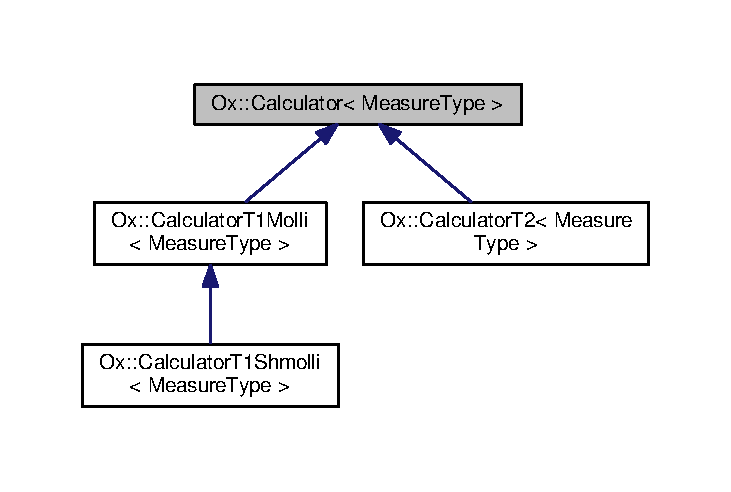
\includegraphics[width=350pt]{class_ox_1_1_calculator__inherit__graph}
\end{center}
\end{figure}
\subsection*{Public Member Functions}
\begin{DoxyCompactItemize}
\item 
virtual int \hyperlink{class_ox_1_1_calculator_a9638894f2ec526b68f46f02122bae0c3}{calculate} ()=0
\item 
virtual int \hyperlink{class_ox_1_1_calculator_a01267c4e842b35f7eacaa9aacdd7e766}{prepare\-To\-Calculate} ()=0
\item 
\hypertarget{class_ox_1_1_calculator_a4b04d48cb906764aa235c387b631dca4}{virtual std\-::map$<$ std\-::string, \\*
Measure\-Type $>$ {\bfseries get\-Results} () const }\label{class_ox_1_1_calculator_a4b04d48cb906764aa235c387b631dca4}

\item 
virtual \hyperlink{class_ox_1_1_model}{Model}$<$ Measure\-Type $>$ $\ast$ \hyperlink{class_ox_1_1_calculator_a5589bf7b93a2d1e106532c35745f4329}{get\-Model} () const 
\item 
virtual \hyperlink{class_ox_1_1_fitter}{Fitter}$<$ Measure\-Type $>$ $\ast$ \hyperlink{class_ox_1_1_calculator_af648a7c6c957c9f51532f15c93147d62}{get\-Fitter} () const 
\item 
\hypertarget{class_ox_1_1_calculator_ad43fbbb3e888e1fa73f95d872a963bac}{virtual \hyperlink{class_ox_1_1_start_point_calculator}{Start\-Point\-Calculator}\\*
$<$ Measure\-Type $>$ $\ast$ {\bfseries get\-Start\-Point\-Calculator} () const }\label{class_ox_1_1_calculator_ad43fbbb3e888e1fa73f95d872a963bac}

\item 
\hypertarget{class_ox_1_1_calculator_a4ee7fdeb4009d2e433ef6a566768eb25}{virtual \hyperlink{class_ox_1_1_sign_calculator}{Sign\-Calculator}\\*
$<$ Measure\-Type $>$ $\ast$ {\bfseries get\-Sign\-Calculator} () const }\label{class_ox_1_1_calculator_a4ee7fdeb4009d2e433ef6a566768eb25}

\item 
\hypertarget{class_ox_1_1_calculator_ab844b24dfedd27d52466203ec0c913fa}{virtual const Measure\-Type $\ast$ {\bfseries get\-Inv\-Times} () const }\label{class_ox_1_1_calculator_ab844b24dfedd27d52466203ec0c913fa}

\item 
\hypertarget{class_ox_1_1_calculator_a6a46eb89732759c2544398f9a694f5c7}{virtual const Measure\-Type $\ast$ {\bfseries get\-Echo\-Times} () const }\label{class_ox_1_1_calculator_a6a46eb89732759c2544398f9a694f5c7}

\item 
\hypertarget{class_ox_1_1_calculator_a2e708f33e09e1e08345bea3024e99ec1}{virtual const Measure\-Type $\ast$ {\bfseries get\-Rep\-Times} () const }\label{class_ox_1_1_calculator_a2e708f33e09e1e08345bea3024e99ec1}

\item 
\hypertarget{class_ox_1_1_calculator_a6698aa9563e9c7d251d4ff73810dd12c}{virtual const Measure\-Type $\ast$ {\bfseries get\-Rel\-Acq\-Times} () const }\label{class_ox_1_1_calculator_a6698aa9563e9c7d251d4ff73810dd12c}

\item 
virtual const Measure\-Type $\ast$ \hyperlink{class_ox_1_1_calculator_ad9a623ee2bfc77732fa891c47c087aa9}{get\-Sig\-Mag} () const 
\item 
virtual const Measure\-Type $\ast$ \hyperlink{class_ox_1_1_calculator_acf6021ef084c24636a344a12627caff5}{get\-Sig\-Pha} () const 
\item 
\hypertarget{class_ox_1_1_calculator_abff843bf55042e78ce613caceef8e6a3}{virtual const Measure\-Type $\ast$ {\bfseries get\-Noise} () const }\label{class_ox_1_1_calculator_abff843bf55042e78ce613caceef8e6a3}

\item 
\hypertarget{class_ox_1_1_calculator_a10c8a3e18079c680cbdf54366d5dfed0}{virtual Measure\-Type $\ast$ {\bfseries get\-Signal} () const }\label{class_ox_1_1_calculator_a10c8a3e18079c680cbdf54366d5dfed0}

\item 
\hypertarget{class_ox_1_1_calculator_ac05783e37c8e6f3f457778ebbfa2e6a5}{virtual Measure\-Type $\ast$ {\bfseries get\-Signs} () const }\label{class_ox_1_1_calculator_ac05783e37c8e6f3f457778ebbfa2e6a5}

\item 
\hypertarget{class_ox_1_1_calculator_aebf55897e1f11cdd3afec75d24c8ea13}{virtual Measure\-Type $\ast$ {\bfseries get\-Start\-Point} ()}\label{class_ox_1_1_calculator_aebf55897e1f11cdd3afec75d24c8ea13}

\item 
\hypertarget{class_ox_1_1_calculator_a8232921e636ebc91a102bc2e95596a7b}{virtual Measure\-Type {\bfseries get\-Mean\-Cut\-Off} () const }\label{class_ox_1_1_calculator_a8232921e636ebc91a102bc2e95596a7b}

\item 
virtual int \hyperlink{class_ox_1_1_calculator_a5e5b6e1af84b8713c833a25d7c0dd90d}{get\-N\-Samples} () const 
\item 
virtual int \hyperlink{class_ox_1_1_calculator_a3a4266dedca7e02707e732a312b85048}{get\-N\-Dims} () const 
\item 
\hypertarget{class_ox_1_1_calculator_ab814b8876ab6ddd7585f73dd23024624}{virtual void {\bfseries set\-Model} (\hyperlink{class_ox_1_1_model}{Model}$<$ Measure\-Type $>$ $\ast$\-\_\-\-Model)}\label{class_ox_1_1_calculator_ab814b8876ab6ddd7585f73dd23024624}

\item 
\hypertarget{class_ox_1_1_calculator_a65d901e63b2f59b77a7dea82eaaa8215}{virtual void {\bfseries set\-Fitter} (\hyperlink{class_ox_1_1_fitter}{Fitter}$<$ Measure\-Type $>$ $\ast$\-\_\-\-Fitter)}\label{class_ox_1_1_calculator_a65d901e63b2f59b77a7dea82eaaa8215}

\item 
\hypertarget{class_ox_1_1_calculator_a9b29545ec9a0e911217f496f7d539471}{virtual void {\bfseries set\-Sign\-Calculator} (\hyperlink{class_ox_1_1_sign_calculator}{Sign\-Calculator}$<$ Measure\-Type $>$ $\ast$\-\_\-\-Sign\-Calculator)}\label{class_ox_1_1_calculator_a9b29545ec9a0e911217f496f7d539471}

\item 
\hypertarget{class_ox_1_1_calculator_a1ea380bc76e9cd19f0a04254ae167230}{virtual void {\bfseries set\-Start\-Point\-Calculator} (\hyperlink{class_ox_1_1_start_point_calculator}{Start\-Point\-Calculator}$<$ Measure\-Type $>$ $\ast$\-\_\-\-Start\-Point\-Calculator)}\label{class_ox_1_1_calculator_a1ea380bc76e9cd19f0a04254ae167230}

\item 
\hypertarget{class_ox_1_1_calculator_a1dcb241d551a06436108a9f4bf916ece}{virtual void {\bfseries set\-Inv\-Times} (const Measure\-Type $\ast$\-\_\-\-Inv\-Times)}\label{class_ox_1_1_calculator_a1dcb241d551a06436108a9f4bf916ece}

\item 
\hypertarget{class_ox_1_1_calculator_aaf50e9d3fae8e95ff981bf15e17bba28}{virtual void {\bfseries set\-Echo\-Times} (const Measure\-Type $\ast$\-\_\-\-Echo\-Times)}\label{class_ox_1_1_calculator_aaf50e9d3fae8e95ff981bf15e17bba28}

\item 
\hypertarget{class_ox_1_1_calculator_a51fb95a1a68b1e14b659761c1f64aaab}{virtual void {\bfseries set\-Sig\-Mag} (const Measure\-Type $\ast$\-\_\-\-Sig\-Mag)}\label{class_ox_1_1_calculator_a51fb95a1a68b1e14b659761c1f64aaab}

\item 
\hypertarget{class_ox_1_1_calculator_a7b753dac0897ee4a5cb9c4d7a21d0926}{virtual void {\bfseries set\-Sig\-Pha} (const Measure\-Type $\ast$\-\_\-\-Sig\-Pha)}\label{class_ox_1_1_calculator_a7b753dac0897ee4a5cb9c4d7a21d0926}

\item 
\hypertarget{class_ox_1_1_calculator_ac78f71339011991131c3b142ae1a9f45}{virtual void {\bfseries set\-Noise} (const Measure\-Type $\ast$\-\_\-\-Noise)}\label{class_ox_1_1_calculator_ac78f71339011991131c3b142ae1a9f45}

\item 
\hypertarget{class_ox_1_1_calculator_ad945e3f4dd3405c940bc8a22ea3f3ee9}{virtual void {\bfseries set\-Mean\-Cut\-Off} (Measure\-Type \-\_\-\-Mean\-Cut\-Off)}\label{class_ox_1_1_calculator_ad945e3f4dd3405c940bc8a22ea3f3ee9}

\item 
virtual void \hyperlink{class_ox_1_1_calculator_a1d0d07b7840883449168448983d43289}{set\-N\-Samples} (int \-\_\-n\-Samples)
\item 
virtual void \hyperlink{class_ox_1_1_calculator_a40c854c0d75685ecc1da531f7400e3b1}{set\-N\-Dims} (int \-\_\-n\-Dims)
\item 
\hypertarget{class_ox_1_1_calculator_a938a4bb0d2bc586bfb6982df28befbbf}{void \hyperlink{class_ox_1_1_calculator_a938a4bb0d2bc586bfb6982df28befbbf}{disp} ()}\label{class_ox_1_1_calculator_a938a4bb0d2bc586bfb6982df28befbbf}

\begin{DoxyCompactList}\small\item\em show me your \hyperlink{class_ox_1_1_model}{Model} \end{DoxyCompactList}\item 
\hypertarget{class_ox_1_1_calculator_acaaddad6379df03cccd825d565c9dd0e}{void \hyperlink{class_ox_1_1_calculator_acaaddad6379df03cccd825d565c9dd0e}{set\-All\-Pointers\-To\-Null} ()}\label{class_ox_1_1_calculator_acaaddad6379df03cccd825d565c9dd0e}

\begin{DoxyCompactList}\small\item\em set all the pointers to zero \end{DoxyCompactList}\item 
\hypertarget{class_ox_1_1_calculator_a4a3762f0c260cb0e34f72e40a7329d27}{\hyperlink{class_ox_1_1_calculator_a4a3762f0c260cb0e34f72e40a7329d27}{Calculator} ()}\label{class_ox_1_1_calculator_a4a3762f0c260cb0e34f72e40a7329d27}

\begin{DoxyCompactList}\small\item\em constructor \end{DoxyCompactList}\item 
\hypertarget{class_ox_1_1_calculator_a600434abcaff13ac70d0d4b06b9df583}{\hyperlink{class_ox_1_1_calculator_a600434abcaff13ac70d0d4b06b9df583}{Calculator} (const \hyperlink{class_ox_1_1_calculator}{Calculator} \&old)}\label{class_ox_1_1_calculator_a600434abcaff13ac70d0d4b06b9df583}

\begin{DoxyCompactList}\small\item\em copy constructor \end{DoxyCompactList}\item 
virtual \hyperlink{class_ox_1_1_calculator}{Calculator}$<$ Measure\-Type $>$ $\ast$ \hyperlink{class_ox_1_1_calculator_aaec48f39f9b0ea1b622485cf25fba484}{new\-By\-Cloning} ()=0
\item 
\hypertarget{class_ox_1_1_calculator_a0e0d0f525a80e54f17ab14e4073d780d}{virtual \hyperlink{class_ox_1_1_calculator_a0e0d0f525a80e54f17ab14e4073d780d}{$\sim$\-Calculator} ()}\label{class_ox_1_1_calculator_a0e0d0f525a80e54f17ab14e4073d780d}

\begin{DoxyCompactList}\small\item\em do not forget about the virtual destructor, see \href{https://stackoverflow.com/questions/461203/when-to-use-virtual-destructors}{\tt https\-://stackoverflow.\-com/questions/461203/when-\/to-\/use-\/virtual-\/destructors} \end{DoxyCompactList}\end{DoxyCompactItemize}
\subsection*{Protected Attributes}
\begin{DoxyCompactItemize}
\item 
\hypertarget{class_ox_1_1_calculator_a37dee4f1bb2fcae66c6710a642fe6d7b}{\hyperlink{class_ox_1_1_model}{Model}$<$ Measure\-Type $>$ $\ast$ {\bfseries \-\_\-\-Model}}\label{class_ox_1_1_calculator_a37dee4f1bb2fcae66c6710a642fe6d7b}

\item 
\hypertarget{class_ox_1_1_calculator_ae00ef8e7db2e9eaa86b8649815246bf9}{\hyperlink{class_ox_1_1_fitter}{Fitter}$<$ Measure\-Type $>$ $\ast$ {\bfseries \-\_\-\-Fitter}}\label{class_ox_1_1_calculator_ae00ef8e7db2e9eaa86b8649815246bf9}

\item 
\hypertarget{class_ox_1_1_calculator_a0655f664d37e70e589bb8526175f19bb}{\hyperlink{class_ox_1_1_sign_calculator}{Sign\-Calculator}$<$ Measure\-Type $>$ $\ast$ {\bfseries \-\_\-\-Sign\-Calculator}}\label{class_ox_1_1_calculator_a0655f664d37e70e589bb8526175f19bb}

\item 
\hypertarget{class_ox_1_1_calculator_a8873b376837e41f40e2a9286a9ea5896}{\hyperlink{class_ox_1_1_start_point_calculator}{Start\-Point\-Calculator}\\*
$<$ Measure\-Type $>$ $\ast$ {\bfseries \-\_\-\-Start\-Point\-Calculator}}\label{class_ox_1_1_calculator_a8873b376837e41f40e2a9286a9ea5896}

\item 
\hypertarget{class_ox_1_1_calculator_ab5f694e40a431677359b6933154eebc0}{const Measure\-Type $\ast$ {\bfseries \-\_\-\-Inv\-Times}}\label{class_ox_1_1_calculator_ab5f694e40a431677359b6933154eebc0}

\item 
\hypertarget{class_ox_1_1_calculator_acc5f2033f9e72e394abae75abdb70076}{const Measure\-Type $\ast$ {\bfseries \-\_\-\-Echo\-Times}}\label{class_ox_1_1_calculator_acc5f2033f9e72e394abae75abdb70076}

\item 
\hypertarget{class_ox_1_1_calculator_acaa46125d5a97260020dcb8e880d8ca4}{const Measure\-Type $\ast$ {\bfseries \-\_\-\-Rep\-Times}}\label{class_ox_1_1_calculator_acaa46125d5a97260020dcb8e880d8ca4}

\item 
\hypertarget{class_ox_1_1_calculator_adc51d44af4e1e42ccda6e49efd618d07}{const Measure\-Type $\ast$ {\bfseries \-\_\-\-Rel\-Acq\-Times}}\label{class_ox_1_1_calculator_adc51d44af4e1e42ccda6e49efd618d07}

\item 
\hypertarget{class_ox_1_1_calculator_a88a92cc098cedb71d7ab4472375e1a71}{const Measure\-Type $\ast$ {\bfseries \-\_\-\-Sig\-Mag}}\label{class_ox_1_1_calculator_a88a92cc098cedb71d7ab4472375e1a71}

\item 
\hypertarget{class_ox_1_1_calculator_a369ce1a35879f24950dd23af0e14761c}{const Measure\-Type $\ast$ {\bfseries \-\_\-\-Sig\-Pha}}\label{class_ox_1_1_calculator_a369ce1a35879f24950dd23af0e14761c}

\item 
\hypertarget{class_ox_1_1_calculator_acb769c5cbf95ad5a59ccc1f587c8c421}{const Measure\-Type $\ast$ {\bfseries \-\_\-\-Noise}}\label{class_ox_1_1_calculator_acb769c5cbf95ad5a59ccc1f587c8c421}

\item 
\hypertarget{class_ox_1_1_calculator_a5bccc8796af4025d3f072406d839d3a6}{Measure\-Type $\ast$ {\bfseries \-\_\-\-Signal}}\label{class_ox_1_1_calculator_a5bccc8796af4025d3f072406d839d3a6}

\item 
\hypertarget{class_ox_1_1_calculator_a00fec572df90a97f103992d5857c46c3}{Measure\-Type $\ast$ {\bfseries \-\_\-\-Signs}}\label{class_ox_1_1_calculator_a00fec572df90a97f103992d5857c46c3}

\item 
\hypertarget{class_ox_1_1_calculator_a133c4c58f97fd13ffccbc7bb20bbd5e5}{Measure\-Type $\ast$ {\bfseries \-\_\-\-Start\-Point}}\label{class_ox_1_1_calculator_a133c4c58f97fd13ffccbc7bb20bbd5e5}

\item 
\hypertarget{class_ox_1_1_calculator_a89303af2e5a0bf1f4f8dae5947bfbab0}{int {\bfseries \-\_\-n\-Samples}}\label{class_ox_1_1_calculator_a89303af2e5a0bf1f4f8dae5947bfbab0}

\item 
\hypertarget{class_ox_1_1_calculator_abf7ad737349c2c4f92c25b3a7a02a063}{int {\bfseries \-\_\-n\-Dims}}\label{class_ox_1_1_calculator_abf7ad737349c2c4f92c25b3a7a02a063}

\item 
\hypertarget{class_ox_1_1_calculator_a27f0852e7c77218109b9fc3df8b92b07}{Measure\-Type {\bfseries \-\_\-\-Mean\-Cut\-Off}}\label{class_ox_1_1_calculator_a27f0852e7c77218109b9fc3df8b92b07}

\item 
\hypertarget{class_ox_1_1_calculator_adae260195d2f056224dbae5e9e34288d}{std\-::map$<$ std\-::string, \\*
Measure\-Type $>$ {\bfseries \-\_\-\-Results}}\label{class_ox_1_1_calculator_adae260195d2f056224dbae5e9e34288d}

\end{DoxyCompactItemize}


\subsection{Member Function Documentation}
\hypertarget{class_ox_1_1_calculator_a9638894f2ec526b68f46f02122bae0c3}{\index{Ox\-::\-Calculator@{Ox\-::\-Calculator}!calculate@{calculate}}
\index{calculate@{calculate}!Ox::Calculator@{Ox\-::\-Calculator}}
\subsubsection[{calculate}]{\setlength{\rightskip}{0pt plus 5cm}template$<$typename Measure\-Type$>$ virtual int {\bf Ox\-::\-Calculator}$<$ Measure\-Type $>$\-::calculate (
\begin{DoxyParamCaption}
{}
\end{DoxyParamCaption}
)\hspace{0.3cm}{\ttfamily [pure virtual]}}}\label{class_ox_1_1_calculator_a9638894f2ec526b68f46f02122bae0c3}
the most important function of this class \begin{DoxyReturn}{Returns}
success/failure 
\end{DoxyReturn}


Implemented in \hyperlink{class_ox_1_1_calculator_t1_shmolli_ac689ebbf27f95f6fa2559cc13a824db0}{Ox\-::\-Calculator\-T1\-Shmolli$<$ Measure\-Type $>$}, \hyperlink{class_ox_1_1_calculator_t2_a8afe4974f3253edea4386a87695607ae}{Ox\-::\-Calculator\-T2$<$ Measure\-Type $>$}, \hyperlink{class_ox_1_1_calculator_t2_truncation_a90077df2125150b62324c83da464b02b}{Ox\-::\-Calculator\-T2\-Truncation$<$ Measure\-Type $>$}, and \hyperlink{class_ox_1_1_calculator_t1_molli_a6f15bc9c026305248c927d62748903bf}{Ox\-::\-Calculator\-T1\-Molli$<$ Measure\-Type $>$}.

\hypertarget{class_ox_1_1_calculator_af648a7c6c957c9f51532f15c93147d62}{\index{Ox\-::\-Calculator@{Ox\-::\-Calculator}!get\-Fitter@{get\-Fitter}}
\index{get\-Fitter@{get\-Fitter}!Ox::Calculator@{Ox\-::\-Calculator}}
\subsubsection[{get\-Fitter}]{\setlength{\rightskip}{0pt plus 5cm}template$<$typename Measure\-Type $>$ {\bf Fitter}$<$ Measure\-Type $>$ $\ast$ {\bf Ox\-::\-Calculator}$<$ Measure\-Type $>$\-::get\-Fitter (
\begin{DoxyParamCaption}
{}
\end{DoxyParamCaption}
) const\hspace{0.3cm}{\ttfamily [virtual]}}}\label{class_ox_1_1_calculator_af648a7c6c957c9f51532f15c93147d62}
/throw exception if \-\_\-\-Fitter == 0 \begin{DoxyReturn}{Returns}

\end{DoxyReturn}
\hypertarget{class_ox_1_1_calculator_a5589bf7b93a2d1e106532c35745f4329}{\index{Ox\-::\-Calculator@{Ox\-::\-Calculator}!get\-Model@{get\-Model}}
\index{get\-Model@{get\-Model}!Ox::Calculator@{Ox\-::\-Calculator}}
\subsubsection[{get\-Model}]{\setlength{\rightskip}{0pt plus 5cm}template$<$typename Measure\-Type $>$ {\bf Model}$<$ Measure\-Type $>$ $\ast$ {\bf Ox\-::\-Calculator}$<$ Measure\-Type $>$\-::get\-Model (
\begin{DoxyParamCaption}
{}
\end{DoxyParamCaption}
) const\hspace{0.3cm}{\ttfamily [virtual]}}}\label{class_ox_1_1_calculator_a5589bf7b93a2d1e106532c35745f4329}
/throw exception if \-\_\-\-Model == 0 \begin{DoxyReturn}{Returns}

\end{DoxyReturn}
\hypertarget{class_ox_1_1_calculator_a3a4266dedca7e02707e732a312b85048}{\index{Ox\-::\-Calculator@{Ox\-::\-Calculator}!get\-N\-Dims@{get\-N\-Dims}}
\index{get\-N\-Dims@{get\-N\-Dims}!Ox::Calculator@{Ox\-::\-Calculator}}
\subsubsection[{get\-N\-Dims}]{\setlength{\rightskip}{0pt plus 5cm}template$<$typename Measure\-Type $>$ int {\bf Ox\-::\-Calculator}$<$ Measure\-Type $>$\-::get\-N\-Dims (
\begin{DoxyParamCaption}
{}
\end{DoxyParamCaption}
) const\hspace{0.3cm}{\ttfamily [virtual]}}}\label{class_ox_1_1_calculator_a3a4266dedca7e02707e732a312b85048}
/throw exception if \-\_\-n\-Dims == 0 \begin{DoxyReturn}{Returns}

\end{DoxyReturn}
\hypertarget{class_ox_1_1_calculator_a5e5b6e1af84b8713c833a25d7c0dd90d}{\index{Ox\-::\-Calculator@{Ox\-::\-Calculator}!get\-N\-Samples@{get\-N\-Samples}}
\index{get\-N\-Samples@{get\-N\-Samples}!Ox::Calculator@{Ox\-::\-Calculator}}
\subsubsection[{get\-N\-Samples}]{\setlength{\rightskip}{0pt plus 5cm}template$<$typename Measure\-Type $>$ int {\bf Ox\-::\-Calculator}$<$ Measure\-Type $>$\-::get\-N\-Samples (
\begin{DoxyParamCaption}
{}
\end{DoxyParamCaption}
) const\hspace{0.3cm}{\ttfamily [virtual]}}}\label{class_ox_1_1_calculator_a5e5b6e1af84b8713c833a25d7c0dd90d}
/throw exception if \-\_\-n\-Samples == 0 \begin{DoxyReturn}{Returns}

\end{DoxyReturn}
\hypertarget{class_ox_1_1_calculator_ad9a623ee2bfc77732fa891c47c087aa9}{\index{Ox\-::\-Calculator@{Ox\-::\-Calculator}!get\-Sig\-Mag@{get\-Sig\-Mag}}
\index{get\-Sig\-Mag@{get\-Sig\-Mag}!Ox::Calculator@{Ox\-::\-Calculator}}
\subsubsection[{get\-Sig\-Mag}]{\setlength{\rightskip}{0pt plus 5cm}template$<$typename Measure\-Type $>$ const Measure\-Type $\ast$ {\bf Ox\-::\-Calculator}$<$ Measure\-Type $>$\-::get\-Sig\-Mag (
\begin{DoxyParamCaption}
{}
\end{DoxyParamCaption}
) const\hspace{0.3cm}{\ttfamily [virtual]}}}\label{class_ox_1_1_calculator_ad9a623ee2bfc77732fa891c47c087aa9}
/throw exception if \-\_\-\-Sig\-Mag == 0 \begin{DoxyReturn}{Returns}

\end{DoxyReturn}
\hypertarget{class_ox_1_1_calculator_acf6021ef084c24636a344a12627caff5}{\index{Ox\-::\-Calculator@{Ox\-::\-Calculator}!get\-Sig\-Pha@{get\-Sig\-Pha}}
\index{get\-Sig\-Pha@{get\-Sig\-Pha}!Ox::Calculator@{Ox\-::\-Calculator}}
\subsubsection[{get\-Sig\-Pha}]{\setlength{\rightskip}{0pt plus 5cm}template$<$typename Measure\-Type $>$ const Measure\-Type $\ast$ {\bf Ox\-::\-Calculator}$<$ Measure\-Type $>$\-::get\-Sig\-Pha (
\begin{DoxyParamCaption}
{}
\end{DoxyParamCaption}
) const\hspace{0.3cm}{\ttfamily [virtual]}}}\label{class_ox_1_1_calculator_acf6021ef084c24636a344a12627caff5}
does not have to be set \begin{DoxyReturn}{Returns}
Sig\-Pha pointer, can be 0 (N\-U\-L\-L) 
\end{DoxyReturn}
\hypertarget{class_ox_1_1_calculator_aaec48f39f9b0ea1b622485cf25fba484}{\index{Ox\-::\-Calculator@{Ox\-::\-Calculator}!new\-By\-Cloning@{new\-By\-Cloning}}
\index{new\-By\-Cloning@{new\-By\-Cloning}!Ox::Calculator@{Ox\-::\-Calculator}}
\subsubsection[{new\-By\-Cloning}]{\setlength{\rightskip}{0pt plus 5cm}template$<$typename Measure\-Type$>$ virtual {\bf Calculator}$<$Measure\-Type$>$$\ast$ {\bf Ox\-::\-Calculator}$<$ Measure\-Type $>$\-::new\-By\-Cloning (
\begin{DoxyParamCaption}
{}
\end{DoxyParamCaption}
)\hspace{0.3cm}{\ttfamily [pure virtual]}}}\label{class_ox_1_1_calculator_aaec48f39f9b0ea1b622485cf25fba484}
cloning \begin{DoxyReturn}{Returns}

\end{DoxyReturn}


Implemented in \hyperlink{class_ox_1_1_calculator_t1_molli_a2a924ff09d446b51542dc246a6a04bd3}{Ox\-::\-Calculator\-T1\-Molli$<$ Measure\-Type $>$}, \hyperlink{class_ox_1_1_calculator_t2_truncation_a6accdab54ee98182f12707786a461c20}{Ox\-::\-Calculator\-T2\-Truncation$<$ Measure\-Type $>$}, \hyperlink{class_ox_1_1_calculator_t2_aaec3b1e6254b67b309c9beedb54ad9e7}{Ox\-::\-Calculator\-T2$<$ Measure\-Type $>$}, and \hyperlink{class_ox_1_1_calculator_t1_shmolli_a1e4e7b6f59b6a0ca4cbe3ed60452b8e9}{Ox\-::\-Calculator\-T1\-Shmolli$<$ Measure\-Type $>$}.

\hypertarget{class_ox_1_1_calculator_a01267c4e842b35f7eacaa9aacdd7e766}{\index{Ox\-::\-Calculator@{Ox\-::\-Calculator}!prepare\-To\-Calculate@{prepare\-To\-Calculate}}
\index{prepare\-To\-Calculate@{prepare\-To\-Calculate}!Ox::Calculator@{Ox\-::\-Calculator}}
\subsubsection[{prepare\-To\-Calculate}]{\setlength{\rightskip}{0pt plus 5cm}template$<$typename Measure\-Type$>$ virtual int {\bf Ox\-::\-Calculator}$<$ Measure\-Type $>$\-::prepare\-To\-Calculate (
\begin{DoxyParamCaption}
{}
\end{DoxyParamCaption}
)\hspace{0.3cm}{\ttfamily [pure virtual]}}}\label{class_ox_1_1_calculator_a01267c4e842b35f7eacaa9aacdd7e766}
processing before calculate is called \begin{DoxyReturn}{Returns}
success/failure 
\end{DoxyReturn}


Implemented in \hyperlink{class_ox_1_1_calculator_t1_shmolli_a6464c63f20ecd9de842d722e5d9d2866}{Ox\-::\-Calculator\-T1\-Shmolli$<$ Measure\-Type $>$}, \hyperlink{class_ox_1_1_calculator_t1_molli_a591ec9658fb5a3e4f48715057cf62b38}{Ox\-::\-Calculator\-T1\-Molli$<$ Measure\-Type $>$}, \hyperlink{class_ox_1_1_calculator_t2_a56e2bcb27465a83dd1a1150b7fe419c8}{Ox\-::\-Calculator\-T2$<$ Measure\-Type $>$}, and \hyperlink{class_ox_1_1_calculator_t2_truncation_a87a5d80163f3909658498c341c7c1a7a}{Ox\-::\-Calculator\-T2\-Truncation$<$ Measure\-Type $>$}.

\hypertarget{class_ox_1_1_calculator_a40c854c0d75685ecc1da531f7400e3b1}{\index{Ox\-::\-Calculator@{Ox\-::\-Calculator}!set\-N\-Dims@{set\-N\-Dims}}
\index{set\-N\-Dims@{set\-N\-Dims}!Ox::Calculator@{Ox\-::\-Calculator}}
\subsubsection[{set\-N\-Dims}]{\setlength{\rightskip}{0pt plus 5cm}template$<$typename Measure\-Type $>$ void {\bf Ox\-::\-Calculator}$<$ Measure\-Type $>$\-::set\-N\-Dims (
\begin{DoxyParamCaption}
\item[{int}]{n\-Dims}
\end{DoxyParamCaption}
)\hspace{0.3cm}{\ttfamily [virtual]}}}\label{class_ox_1_1_calculator_a40c854c0d75685ecc1da531f7400e3b1}
\-\_\-\-Start\-Point is allocated here!!! 
\begin{DoxyParams}{Parameters}
{\em \-\_\-n\-Dims} & \\
\hline
\end{DoxyParams}
\hypertarget{class_ox_1_1_calculator_a1d0d07b7840883449168448983d43289}{\index{Ox\-::\-Calculator@{Ox\-::\-Calculator}!set\-N\-Samples@{set\-N\-Samples}}
\index{set\-N\-Samples@{set\-N\-Samples}!Ox::Calculator@{Ox\-::\-Calculator}}
\subsubsection[{set\-N\-Samples}]{\setlength{\rightskip}{0pt plus 5cm}template$<$typename Measure\-Type $>$ void {\bf Ox\-::\-Calculator}$<$ Measure\-Type $>$\-::set\-N\-Samples (
\begin{DoxyParamCaption}
\item[{int}]{\-\_\-n\-Samples}
\end{DoxyParamCaption}
)\hspace{0.3cm}{\ttfamily [virtual]}}}\label{class_ox_1_1_calculator_a1d0d07b7840883449168448983d43289}
\-\_\-\-Signal and \-\_\-\-Signs are allocated here!!! 
\begin{DoxyParams}{Parameters}
{\em \-\_\-n\-Samples} & \\
\hline
\end{DoxyParams}


The documentation for this class was generated from the following files\-:\begin{DoxyCompactItemize}
\item 
lib/\hyperlink{_ox_calculator_8h}{Ox\-Calculator.\-h}\item 
lib/\hyperlink{_ox_calculator_8hxx}{Ox\-Calculator.\-hxx}\end{DoxyCompactItemize}

\hypertarget{class_calculator_t1}{\section{Calculator\-T1 Class Reference}
\label{class_calculator_t1}\index{Calculator\-T1@{Calculator\-T1}}
}


{\ttfamily \#include $<$Ox\-Calculator.\-h$>$}



\subsection{Detailed Description}

\begin{DoxyTemplParams}{Template Parameters}
{\em Measure\-Type} & \\
\hline
\end{DoxyTemplParams}


The documentation for this class was generated from the following file\-:\begin{DoxyCompactItemize}
\item 
lib/\hyperlink{_ox_calculator_8h}{Ox\-Calculator.\-h}\end{DoxyCompactItemize}

\hypertarget{class_ox_1_1_calculator_t1_molli}{\section{Ox\-:\-:Calculator\-T1\-Molli$<$ Measure\-Type $>$ Class Template Reference}
\label{class_ox_1_1_calculator_t1_molli}\index{Ox\-::\-Calculator\-T1\-Molli$<$ Measure\-Type $>$@{Ox\-::\-Calculator\-T1\-Molli$<$ Measure\-Type $>$}}
}


{\ttfamily \#include $<$Ox\-Calculator\-T1\-Molli.\-h$>$}



Inheritance diagram for Ox\-:\-:Calculator\-T1\-Molli$<$ Measure\-Type $>$\-:
\nopagebreak
\begin{figure}[H]
\begin{center}
\leavevmode
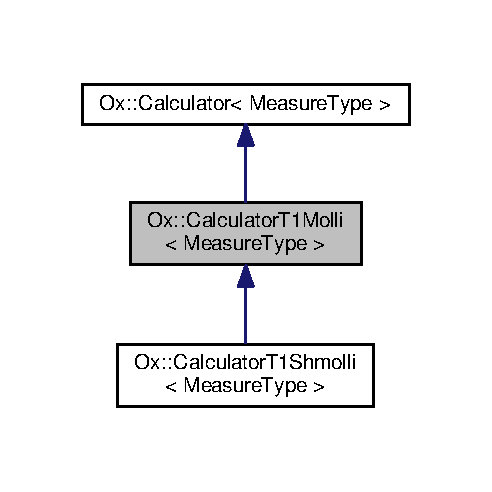
\includegraphics[width=216pt]{class_ox_1_1_calculator_t1_molli__inherit__graph}
\end{center}
\end{figure}


Collaboration diagram for Ox\-:\-:Calculator\-T1\-Molli$<$ Measure\-Type $>$\-:
\nopagebreak
\begin{figure}[H]
\begin{center}
\leavevmode
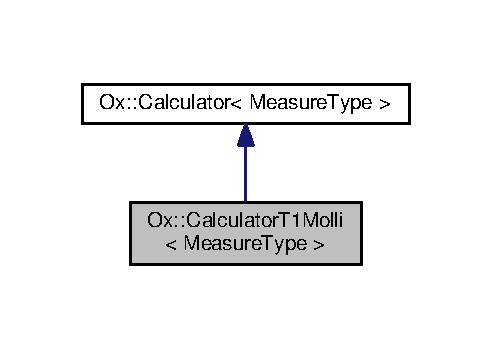
\includegraphics[width=216pt]{class_ox_1_1_calculator_t1_molli__coll__graph}
\end{center}
\end{figure}
\subsection*{Public Member Functions}
\begin{DoxyCompactItemize}
\item 
virtual int \hyperlink{class_ox_1_1_calculator_t1_molli_a6f15bc9c026305248c927d62748903bf}{calculate} ()
\item 
virtual \hyperlink{struct_ox_1_1_calculator_t1_results}{Calculator\-T1\-Results}\\*
$<$ Measure\-Type $>$ \hyperlink{class_ox_1_1_calculator_t1_molli_a9cb84f5e8680e1bf6c3543846fc90c4d}{calculate\-Molli} (int n\-Samples, const Measure\-Type $\ast$inv\-Times, Measure\-Type $\ast$signal, Measure\-Type $\ast$signs)
\item 
Measure\-Type \hyperlink{class_ox_1_1_calculator_t1_molli_a9c9238dd8a96e06d3e0a96810377b90b}{calculate\-R2\-Abs\-From\-Model} (int n\-Samples, const Measure\-Type $\ast$inv\-Times, const Measure\-Type $\ast$signal, const Measure\-Type $\ast$parameters)
\item 
int \hyperlink{class_ox_1_1_calculator_t1_molli_a030582bca754a7b81febfae53fe0c10c}{calculate\-Covariance\-Matrix} (const Measure\-Type $\ast$parameters, Measure\-Type $\ast$covariance\-Matrix)
\item 
int \hyperlink{class_ox_1_1_calculator_t1_molli_aec374fc512aa3b109138f0c16c53a171}{calculate\-Inv\-Covariance\-Matrix} (const Measure\-Type $\ast$inv\-Times, const Measure\-Type $\ast$residuals, const Measure\-Type $\ast$parameters, Measure\-Type $\ast$inv\-Covariance\-Matrix)
\item 
bool \hyperlink{class_ox_1_1_calculator_t1_molli_a06d8579492ee063b129b489e638333be}{get\-Do\-Calculate\-S\-D\-Map} () const 
\item 
void \hyperlink{class_ox_1_1_calculator_t1_molli_a65a51dcadaafdefc576201de535f8810}{set\-Do\-Calculate\-S\-D\-Map} (bool \-\_\-\-Do\-Calculate\-S\-D\-Map)
\item 
\hyperlink{class_ox_1_1_calculator_t1_molli_ab1892de078822ea106fcaebcf81047be}{Calculator\-T1\-Molli} ()
\item 
virtual \hyperlink{class_ox_1_1_calculator_t1}{Calculator\-T1}\\*
$<$ Measure\-Type $>$ $\ast$ \hyperlink{class_ox_1_1_calculator_t1_molli_ae0fde362fbe16c4c40dee96330b4a676}{new\-By\-Cloning} ()
\end{DoxyCompactItemize}
\subsection*{Protected Attributes}
\begin{DoxyCompactItemize}
\item 
\hypertarget{class_ox_1_1_calculator_t1_molli_adb4f50cdf9dabf4890b4d28194d0522b}{double {\bfseries Max\-T\-I\-For\-Sign\-Invert}}\label{class_ox_1_1_calculator_t1_molli_adb4f50cdf9dabf4890b4d28194d0522b}

\item 
\hypertarget{class_ox_1_1_calculator_t1_molli_adbe23b503f5695ff35734d2c20972277}{bool {\bfseries \-\_\-\-Do\-Calculate\-S\-D\-Map}}\label{class_ox_1_1_calculator_t1_molli_adbe23b503f5695ff35734d2c20972277}

\end{DoxyCompactItemize}
\subsection*{Additional Inherited Members}


\subsection{Detailed Description}
\subsubsection*{template$<$typename Measure\-Type$>$class Ox\-::\-Calculator\-T1\-Molli$<$ Measure\-Type $>$}


\begin{DoxyTemplParams}{Template Parameters}
{\em Measure\-Type} & \\
\hline
\end{DoxyTemplParams}


\subsection{Constructor \& Destructor Documentation}
\hypertarget{class_ox_1_1_calculator_t1_molli_ab1892de078822ea106fcaebcf81047be}{\index{Ox\-::\-Calculator\-T1\-Molli@{Ox\-::\-Calculator\-T1\-Molli}!Calculator\-T1\-Molli@{Calculator\-T1\-Molli}}
\index{Calculator\-T1\-Molli@{Calculator\-T1\-Molli}!Ox::CalculatorT1Molli@{Ox\-::\-Calculator\-T1\-Molli}}
\subsubsection[{Calculator\-T1\-Molli}]{\setlength{\rightskip}{0pt plus 5cm}template$<$typename Measure\-Type$>$ {\bf Ox\-::\-Calculator\-T1\-Molli}$<$ Measure\-Type $>$\-::{\bf Calculator\-T1\-Molli} (
\begin{DoxyParamCaption}
{}
\end{DoxyParamCaption}
)\hspace{0.3cm}{\ttfamily [inline]}}}\label{class_ox_1_1_calculator_t1_molli_ab1892de078822ea106fcaebcf81047be}
constructor 

\subsection{Member Function Documentation}
\hypertarget{class_ox_1_1_calculator_t1_molli_a6f15bc9c026305248c927d62748903bf}{\index{Ox\-::\-Calculator\-T1\-Molli@{Ox\-::\-Calculator\-T1\-Molli}!calculate@{calculate}}
\index{calculate@{calculate}!Ox::CalculatorT1Molli@{Ox\-::\-Calculator\-T1\-Molli}}
\subsubsection[{calculate}]{\setlength{\rightskip}{0pt plus 5cm}template$<$typename Measure\-Type $>$ int {\bf Ox\-::\-Calculator\-T1\-Molli}$<$ Measure\-Type $>$\-::calculate (
\begin{DoxyParamCaption}
{}
\end{DoxyParamCaption}
)\hspace{0.3cm}{\ttfamily [virtual]}}}\label{class_ox_1_1_calculator_t1_molli_a6f15bc9c026305248c927d62748903bf}
calling \hyperlink{class_ox_1_1_calculator_t1_molli_a9cb84f5e8680e1bf6c3543846fc90c4d}{calculate\-Molli(int n\-Samples, const Measure\-Type$\ast$ inv\-Times, Measure\-Type$\ast$ signal, Measure\-Type$\ast$ signs)} \begin{DoxyReturn}{Returns}
success/failure 
\end{DoxyReturn}


Implements \hyperlink{class_ox_1_1_calculator_t1_ab8d5ec3f03e070ca11d3accb59a92299}{Ox\-::\-Calculator\-T1$<$ Measure\-Type $>$}.



Reimplemented in \hyperlink{class_ox_1_1_calculator_t1_shmolli_ac689ebbf27f95f6fa2559cc13a824db0}{Ox\-::\-Calculator\-T1\-Shmolli$<$ Measure\-Type $>$}.

\hypertarget{class_ox_1_1_calculator_t1_molli_a030582bca754a7b81febfae53fe0c10c}{\index{Ox\-::\-Calculator\-T1\-Molli@{Ox\-::\-Calculator\-T1\-Molli}!calculate\-Covariance\-Matrix@{calculate\-Covariance\-Matrix}}
\index{calculate\-Covariance\-Matrix@{calculate\-Covariance\-Matrix}!Ox::CalculatorT1Molli@{Ox\-::\-Calculator\-T1\-Molli}}
\subsubsection[{calculate\-Covariance\-Matrix}]{\setlength{\rightskip}{0pt plus 5cm}template$<$typename Measure\-Type $>$ int {\bf Ox\-::\-Calculator\-T1\-Molli}$<$ Measure\-Type $>$\-::calculate\-Covariance\-Matrix (
\begin{DoxyParamCaption}
\item[{const Measure\-Type $\ast$}]{parameters, }
\item[{Measure\-Type $\ast$}]{covariance\-Matrix}
\end{DoxyParamCaption}
)}}\label{class_ox_1_1_calculator_t1_molli_a030582bca754a7b81febfae53fe0c10c}
calculate covariance matrix needed for S\-D estimation 
\begin{DoxyParams}{Parameters}
{\em parameters} & \\
\hline
{\em covariance\-Matrix} & \\
\hline
\end{DoxyParams}
\begin{DoxyReturn}{Returns}

\end{DoxyReturn}
\hypertarget{class_ox_1_1_calculator_t1_molli_aec374fc512aa3b109138f0c16c53a171}{\index{Ox\-::\-Calculator\-T1\-Molli@{Ox\-::\-Calculator\-T1\-Molli}!calculate\-Inv\-Covariance\-Matrix@{calculate\-Inv\-Covariance\-Matrix}}
\index{calculate\-Inv\-Covariance\-Matrix@{calculate\-Inv\-Covariance\-Matrix}!Ox::CalculatorT1Molli@{Ox\-::\-Calculator\-T1\-Molli}}
\subsubsection[{calculate\-Inv\-Covariance\-Matrix}]{\setlength{\rightskip}{0pt plus 5cm}template$<$typename Measure\-Type $>$ int {\bf Ox\-::\-Calculator\-T1\-Molli}$<$ Measure\-Type $>$\-::calculate\-Inv\-Covariance\-Matrix (
\begin{DoxyParamCaption}
\item[{const Measure\-Type $\ast$}]{inv\-Times, }
\item[{const Measure\-Type $\ast$}]{residuals, }
\item[{const Measure\-Type $\ast$}]{parameters, }
\item[{Measure\-Type $\ast$}]{inv\-Covariance\-Matrix}
\end{DoxyParamCaption}
)}}\label{class_ox_1_1_calculator_t1_molli_aec374fc512aa3b109138f0c16c53a171}
calculate inverse covariance matrix needed for S\-D estimation 
\begin{DoxyParams}{Parameters}
{\em inv\-Times} & \\
\hline
{\em residuals} & \\
\hline
{\em parameters} & \\
\hline
{\em inv\-Covariance\-Matrix} & \\
\hline
\end{DoxyParams}
\begin{DoxyReturn}{Returns}

\end{DoxyReturn}
\hypertarget{class_ox_1_1_calculator_t1_molli_a9cb84f5e8680e1bf6c3543846fc90c4d}{\index{Ox\-::\-Calculator\-T1\-Molli@{Ox\-::\-Calculator\-T1\-Molli}!calculate\-Molli@{calculate\-Molli}}
\index{calculate\-Molli@{calculate\-Molli}!Ox::CalculatorT1Molli@{Ox\-::\-Calculator\-T1\-Molli}}
\subsubsection[{calculate\-Molli}]{\setlength{\rightskip}{0pt plus 5cm}template$<$typename Measure\-Type $>$ {\bf Calculator\-T1\-Results}$<$ Measure\-Type $>$ {\bf Ox\-::\-Calculator\-T1\-Molli}$<$ Measure\-Type $>$\-::calculate\-Molli (
\begin{DoxyParamCaption}
\item[{int}]{n\-Samples, }
\item[{const Measure\-Type $\ast$}]{inv\-Times, }
\item[{Measure\-Type $\ast$}]{signal, }
\item[{Measure\-Type $\ast$}]{signs}
\end{DoxyParamCaption}
)\hspace{0.3cm}{\ttfamily [virtual]}}}\label{class_ox_1_1_calculator_t1_molli_a9cb84f5e8680e1bf6c3543846fc90c4d}
The most important function of this class It has all the input parameters so that I can call it from the shmolli class 
\begin{DoxyParams}{Parameters}
{\em n\-Samples} & \\
\hline
{\em inv\-Times} & \\
\hline
{\em signal} & \\
\hline
{\em signs} & \\
\hline
\end{DoxyParams}
\begin{DoxyReturn}{Returns}
success/failure 
\end{DoxyReturn}
\hypertarget{class_ox_1_1_calculator_t1_molli_a9c9238dd8a96e06d3e0a96810377b90b}{\index{Ox\-::\-Calculator\-T1\-Molli@{Ox\-::\-Calculator\-T1\-Molli}!calculate\-R2\-Abs\-From\-Model@{calculate\-R2\-Abs\-From\-Model}}
\index{calculate\-R2\-Abs\-From\-Model@{calculate\-R2\-Abs\-From\-Model}!Ox::CalculatorT1Molli@{Ox\-::\-Calculator\-T1\-Molli}}
\subsubsection[{calculate\-R2\-Abs\-From\-Model}]{\setlength{\rightskip}{0pt plus 5cm}template$<$typename Measure\-Type $>$ Measure\-Type {\bf Ox\-::\-Calculator\-T1\-Molli}$<$ Measure\-Type $>$\-::calculate\-R2\-Abs\-From\-Model (
\begin{DoxyParamCaption}
\item[{int}]{n\-Samples, }
\item[{const Measure\-Type $\ast$}]{inv\-Times, }
\item[{const Measure\-Type $\ast$}]{signal, }
\item[{const Measure\-Type $\ast$}]{parameters}
\end{DoxyParamCaption}
)}}\label{class_ox_1_1_calculator_t1_molli_a9c9238dd8a96e06d3e0a96810377b90b}
Calculate goodness of fit map 
\begin{DoxyParams}{Parameters}
{\em n\-Samples} & \\
\hline
{\em inv\-Times} & \\
\hline
{\em signal} & \\
\hline
{\em parameters} & \\
\hline
\end{DoxyParams}
\begin{DoxyReturn}{Returns}

\end{DoxyReturn}
\hypertarget{class_ox_1_1_calculator_t1_molli_a06d8579492ee063b129b489e638333be}{\index{Ox\-::\-Calculator\-T1\-Molli@{Ox\-::\-Calculator\-T1\-Molli}!get\-Do\-Calculate\-S\-D\-Map@{get\-Do\-Calculate\-S\-D\-Map}}
\index{get\-Do\-Calculate\-S\-D\-Map@{get\-Do\-Calculate\-S\-D\-Map}!Ox::CalculatorT1Molli@{Ox\-::\-Calculator\-T1\-Molli}}
\subsubsection[{get\-Do\-Calculate\-S\-D\-Map}]{\setlength{\rightskip}{0pt plus 5cm}template$<$typename Measure\-Type $>$ bool {\bf Ox\-::\-Calculator\-T1\-Molli}$<$ Measure\-Type $>$\-::get\-Do\-Calculate\-S\-D\-Map (
\begin{DoxyParamCaption}
{}
\end{DoxyParamCaption}
) const}}\label{class_ox_1_1_calculator_t1_molli_a06d8579492ee063b129b489e638333be}
\begin{DoxyReturn}{Returns}

\end{DoxyReturn}
\hypertarget{class_ox_1_1_calculator_t1_molli_ae0fde362fbe16c4c40dee96330b4a676}{\index{Ox\-::\-Calculator\-T1\-Molli@{Ox\-::\-Calculator\-T1\-Molli}!new\-By\-Cloning@{new\-By\-Cloning}}
\index{new\-By\-Cloning@{new\-By\-Cloning}!Ox::CalculatorT1Molli@{Ox\-::\-Calculator\-T1\-Molli}}
\subsubsection[{new\-By\-Cloning}]{\setlength{\rightskip}{0pt plus 5cm}template$<$typename Measure\-Type$>$ virtual {\bf Calculator\-T1}$<$Measure\-Type$>$$\ast$ {\bf Ox\-::\-Calculator\-T1\-Molli}$<$ Measure\-Type $>$\-::new\-By\-Cloning (
\begin{DoxyParamCaption}
{}
\end{DoxyParamCaption}
)\hspace{0.3cm}{\ttfamily [inline]}, {\ttfamily [virtual]}}}\label{class_ox_1_1_calculator_t1_molli_ae0fde362fbe16c4c40dee96330b4a676}
cloning \begin{DoxyReturn}{Returns}

\end{DoxyReturn}


Implements \hyperlink{class_ox_1_1_calculator_t1_a0db8102b4dad27368667e6ec89c6e4f3}{Ox\-::\-Calculator\-T1$<$ Measure\-Type $>$}.



Reimplemented in \hyperlink{class_ox_1_1_calculator_t1_shmolli_a5fa5fd5685a5566e605a1ee93569ac29}{Ox\-::\-Calculator\-T1\-Shmolli$<$ Measure\-Type $>$}.

\hypertarget{class_ox_1_1_calculator_t1_molli_a65a51dcadaafdefc576201de535f8810}{\index{Ox\-::\-Calculator\-T1\-Molli@{Ox\-::\-Calculator\-T1\-Molli}!set\-Do\-Calculate\-S\-D\-Map@{set\-Do\-Calculate\-S\-D\-Map}}
\index{set\-Do\-Calculate\-S\-D\-Map@{set\-Do\-Calculate\-S\-D\-Map}!Ox::CalculatorT1Molli@{Ox\-::\-Calculator\-T1\-Molli}}
\subsubsection[{set\-Do\-Calculate\-S\-D\-Map}]{\setlength{\rightskip}{0pt plus 5cm}template$<$typename Measure\-Type $>$ void {\bf Ox\-::\-Calculator\-T1\-Molli}$<$ Measure\-Type $>$\-::set\-Do\-Calculate\-S\-D\-Map (
\begin{DoxyParamCaption}
\item[{bool}]{\-\_\-\-Do\-Calculate\-S\-D\-Map}
\end{DoxyParamCaption}
)}}\label{class_ox_1_1_calculator_t1_molli_a65a51dcadaafdefc576201de535f8810}

\begin{DoxyParams}{Parameters}
{\em \-\_\-\-Do\-Calculate\-S\-D\-Map} & \\
\hline
\end{DoxyParams}


The documentation for this class was generated from the following files\-:\begin{DoxyCompactItemize}
\item 
lib/\hyperlink{_ox_calculator_t1_molli_8h}{Ox\-Calculator\-T1\-Molli.\-h}\item 
lib/\hyperlink{_ox_calculator_t1_molli_8hxx}{Ox\-Calculator\-T1\-Molli.\-hxx}\end{DoxyCompactItemize}

\hypertarget{class_ox_1_1_calculator_t1_shmolli}{}\section{Ox\+:\+:Calculator\+T1\+Shmolli$<$ Measure\+Type $>$ Class Template Reference}
\label{class_ox_1_1_calculator_t1_shmolli}\index{Ox\+::\+Calculator\+T1\+Shmolli$<$ Measure\+Type $>$@{Ox\+::\+Calculator\+T1\+Shmolli$<$ Measure\+Type $>$}}


Inheritance diagram for Ox\+:\+:Calculator\+T1\+Shmolli$<$ Measure\+Type $>$\+:
\nopagebreak
\begin{figure}[H]
\begin{center}
\leavevmode
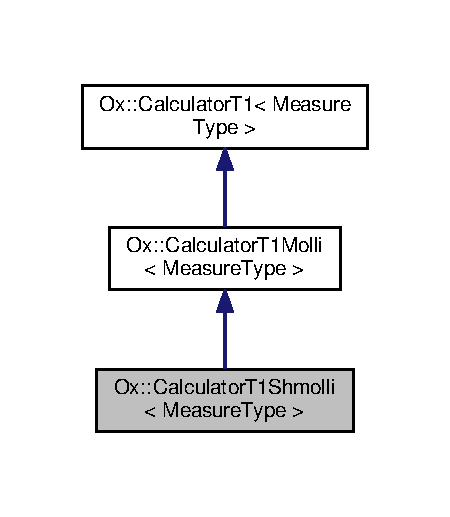
\includegraphics[width=237pt]{class_ox_1_1_calculator_t1_shmolli__inherit__graph}
\end{center}
\end{figure}


Collaboration diagram for Ox\+:\+:Calculator\+T1\+Shmolli$<$ Measure\+Type $>$\+:
\nopagebreak
\begin{figure}[H]
\begin{center}
\leavevmode
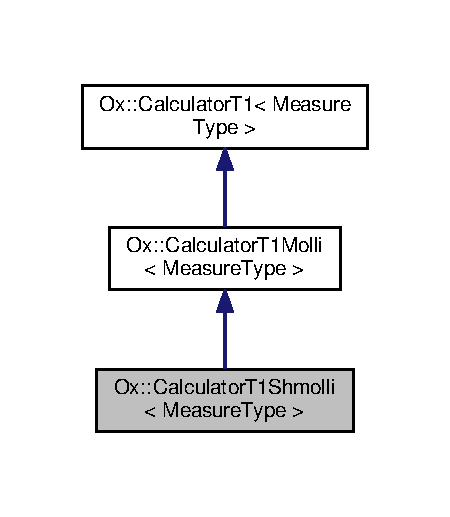
\includegraphics[width=237pt]{class_ox_1_1_calculator_t1_shmolli__coll__graph}
\end{center}
\end{figure}
\subsection*{Public Member Functions}
\begin{DoxyCompactItemize}
\item 
\hyperlink{class_ox_1_1_calculator_t1_shmolli_a693169987cfe715b58c7502b306230f5}{Calculator\+T1\+Shmolli} ()
\item 
virtual \hyperlink{class_ox_1_1_calculator}{Calculator}$<$ Measure\+Type $>$ $\ast$ \hyperlink{class_ox_1_1_calculator_t1_shmolli_a1e4e7b6f59b6a0ca4cbe3ed60452b8e9}{new\+By\+Cloning} ()
\item 
virtual int \hyperlink{class_ox_1_1_calculator_t1_shmolli_a6464c63f20ecd9de842d722e5d9d2866}{prepare\+To\+Calculate} ()
\item 
int {\bfseries get\+Start\+Point\+S\+K\+P\+Shmolli} (const Measure\+Type $\ast$inv\+Times5, const Measure\+Type $\ast$inv\+Times6, const Measure\+Type $\ast$inv\+Times7, const Measure\+Type $\ast$sig\+Mag5, const Measure\+Type $\ast$sig\+Mag6, const Measure\+Type $\ast$sig\+Mag7, const Measure\+Type $\ast$signs5, const Measure\+Type $\ast$signs6, const Measure\+Type $\ast$signs7)\hypertarget{class_ox_1_1_calculator_t1_shmolli_ab44f84d453405c2c61094fc4cd53449c}{}\label{class_ox_1_1_calculator_t1_shmolli_ab44f84d453405c2c61094fc4cd53449c}

\item 
int \hyperlink{class_ox_1_1_calculator_t1_shmolli_a2c4444b1aa40e3f01b7cf0b8e7f7672b}{calculate\+T\+R\+Raverage\+HB} ()
\item 
virtual int \hyperlink{class_ox_1_1_calculator_t1_shmolli_ac689ebbf27f95f6fa2559cc13a824db0}{calculate} ()
\item 
int {\bfseries get\+Shmolli\+Samples} (const Measure\+Type $\ast$in\+Array, Measure\+Type $\ast$out\+Array5, Measure\+Type $\ast$out\+Array6, Measure\+Type $\ast$out\+Array7)\hypertarget{class_ox_1_1_calculator_t1_shmolli_a5e2d8b626c05aebbf816cb0594295b77}{}\label{class_ox_1_1_calculator_t1_shmolli_a5e2d8b626c05aebbf816cb0594295b77}

\end{DoxyCompactItemize}
\subsection*{Additional Inherited Members}


\subsection{Constructor \& Destructor Documentation}
\index{Ox\+::\+Calculator\+T1\+Shmolli@{Ox\+::\+Calculator\+T1\+Shmolli}!Calculator\+T1\+Shmolli@{Calculator\+T1\+Shmolli}}
\index{Calculator\+T1\+Shmolli@{Calculator\+T1\+Shmolli}!Ox\+::\+Calculator\+T1\+Shmolli@{Ox\+::\+Calculator\+T1\+Shmolli}}
\subsubsection[{\texorpdfstring{Calculator\+T1\+Shmolli()}{CalculatorT1Shmolli()}}]{\setlength{\rightskip}{0pt plus 5cm}template$<$typename Measure\+Type$>$ {\bf Ox\+::\+Calculator\+T1\+Shmolli}$<$ Measure\+Type $>$\+::{\bf Calculator\+T1\+Shmolli} (
\begin{DoxyParamCaption}
{}
\end{DoxyParamCaption}
)\hspace{0.3cm}{\ttfamily [inline]}}\hypertarget{class_ox_1_1_calculator_t1_shmolli_a693169987cfe715b58c7502b306230f5}{}\label{class_ox_1_1_calculator_t1_shmolli_a693169987cfe715b58c7502b306230f5}
constructor 

\subsection{Member Function Documentation}
\index{Ox\+::\+Calculator\+T1\+Shmolli@{Ox\+::\+Calculator\+T1\+Shmolli}!calculate@{calculate}}
\index{calculate@{calculate}!Ox\+::\+Calculator\+T1\+Shmolli@{Ox\+::\+Calculator\+T1\+Shmolli}}
\subsubsection[{\texorpdfstring{calculate()}{calculate()}}]{\setlength{\rightskip}{0pt plus 5cm}template$<$typename Measure\+Type $>$ int {\bf Ox\+::\+Calculator\+T1\+Shmolli}$<$ Measure\+Type $>$\+::calculate (
\begin{DoxyParamCaption}
{}
\end{DoxyParamCaption}
)\hspace{0.3cm}{\ttfamily [virtual]}}\hypertarget{class_ox_1_1_calculator_t1_shmolli_ac689ebbf27f95f6fa2559cc13a824db0}{}\label{class_ox_1_1_calculator_t1_shmolli_ac689ebbf27f95f6fa2559cc13a824db0}
the most important function of this class \begin{DoxyReturn}{Returns}
success/failure 
\end{DoxyReturn}


Reimplemented from \hyperlink{class_ox_1_1_calculator_t1_with_sign_check_ae5b9cb33d60b5c4d96f8890b3ca991c4}{Ox\+::\+Calculator\+T1\+With\+Sign\+Check$<$ Measure\+Type $>$}.

\index{Ox\+::\+Calculator\+T1\+Shmolli@{Ox\+::\+Calculator\+T1\+Shmolli}!calculate\+T\+R\+Raverage\+HB@{calculate\+T\+R\+Raverage\+HB}}
\index{calculate\+T\+R\+Raverage\+HB@{calculate\+T\+R\+Raverage\+HB}!Ox\+::\+Calculator\+T1\+Shmolli@{Ox\+::\+Calculator\+T1\+Shmolli}}
\subsubsection[{\texorpdfstring{calculate\+T\+R\+Raverage\+H\+B()}{calculateTRRaverageHB()}}]{\setlength{\rightskip}{0pt plus 5cm}template$<$typename Measure\+Type $>$ int {\bf Ox\+::\+Calculator\+T1\+Shmolli}$<$ Measure\+Type $>$\+::calculate\+T\+R\+Raverage\+HB (
\begin{DoxyParamCaption}
{}
\end{DoxyParamCaption}
)}\hypertarget{class_ox_1_1_calculator_t1_shmolli_a2c4444b1aa40e3f01b7cf0b8e7f7672b}{}\label{class_ox_1_1_calculator_t1_shmolli_a2c4444b1aa40e3f01b7cf0b8e7f7672b}
Average heart rate (distance between dwo R waves) T\+RR is used in Sh\+M\+O\+L\+LI conditions \begin{DoxyReturn}{Returns}

\end{DoxyReturn}
\index{Ox\+::\+Calculator\+T1\+Shmolli@{Ox\+::\+Calculator\+T1\+Shmolli}!new\+By\+Cloning@{new\+By\+Cloning}}
\index{new\+By\+Cloning@{new\+By\+Cloning}!Ox\+::\+Calculator\+T1\+Shmolli@{Ox\+::\+Calculator\+T1\+Shmolli}}
\subsubsection[{\texorpdfstring{new\+By\+Cloning()}{newByCloning()}}]{\setlength{\rightskip}{0pt plus 5cm}template$<$typename Measure\+Type$>$ virtual {\bf Calculator}$<$Measure\+Type$>$$\ast$ {\bf Ox\+::\+Calculator\+T1\+Shmolli}$<$ Measure\+Type $>$\+::new\+By\+Cloning (
\begin{DoxyParamCaption}
{}
\end{DoxyParamCaption}
)\hspace{0.3cm}{\ttfamily [inline]}, {\ttfamily [virtual]}}\hypertarget{class_ox_1_1_calculator_t1_shmolli_a1e4e7b6f59b6a0ca4cbe3ed60452b8e9}{}\label{class_ox_1_1_calculator_t1_shmolli_a1e4e7b6f59b6a0ca4cbe3ed60452b8e9}
cloning \begin{DoxyReturn}{Returns}

\end{DoxyReturn}


Reimplemented from \hyperlink{class_ox_1_1_calculator_t1_with_sign_check_a59e5be9935b9c235f4958a461fda081e}{Ox\+::\+Calculator\+T1\+With\+Sign\+Check$<$ Measure\+Type $>$}.

\index{Ox\+::\+Calculator\+T1\+Shmolli@{Ox\+::\+Calculator\+T1\+Shmolli}!prepare\+To\+Calculate@{prepare\+To\+Calculate}}
\index{prepare\+To\+Calculate@{prepare\+To\+Calculate}!Ox\+::\+Calculator\+T1\+Shmolli@{Ox\+::\+Calculator\+T1\+Shmolli}}
\subsubsection[{\texorpdfstring{prepare\+To\+Calculate()}{prepareToCalculate()}}]{\setlength{\rightskip}{0pt plus 5cm}template$<$typename Measure\+Type $>$ int {\bf Ox\+::\+Calculator\+T1\+Shmolli}$<$ Measure\+Type $>$\+::prepare\+To\+Calculate (
\begin{DoxyParamCaption}
{}
\end{DoxyParamCaption}
)\hspace{0.3cm}{\ttfamily [virtual]}}\hypertarget{class_ox_1_1_calculator_t1_shmolli_a6464c63f20ecd9de842d722e5d9d2866}{}\label{class_ox_1_1_calculator_t1_shmolli_a6464c63f20ecd9de842d722e5d9d2866}
prepare\+To\+Calculate \begin{DoxyReturn}{Returns}

\end{DoxyReturn}


Reimplemented from \hyperlink{class_ox_1_1_calculator_t1_with_sign_check_ad93dba810e34daf87ac35839cb0ff671}{Ox\+::\+Calculator\+T1\+With\+Sign\+Check$<$ Measure\+Type $>$}.



The documentation for this class was generated from the following files\+:\begin{DoxyCompactItemize}
\item 
lib/\hyperlink{_ox_calculator_t1_shmolli_8h}{Ox\+Calculator\+T1\+Shmolli.\+h}\item 
lib/\hyperlink{_ox_calculator_t1_shmolli_8hxx}{Ox\+Calculator\+T1\+Shmolli.\+hxx}\end{DoxyCompactItemize}

\hypertarget{class_ox_1_1_calculator_t2}{\section{Ox\-:\-:Calculator\-T2$<$ Measure\-Type $>$ Class Template Reference}
\label{class_ox_1_1_calculator_t2}\index{Ox\-::\-Calculator\-T2$<$ Measure\-Type $>$@{Ox\-::\-Calculator\-T2$<$ Measure\-Type $>$}}
}


{\ttfamily \#include $<$Ox\-Calculator\-T2.\-h$>$}



Inheritance diagram for Ox\-:\-:Calculator\-T2$<$ Measure\-Type $>$\-:
\nopagebreak
\begin{figure}[H]
\begin{center}
\leavevmode
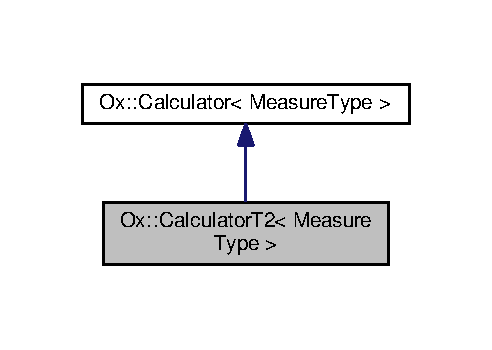
\includegraphics[width=236pt]{class_ox_1_1_calculator_t2__inherit__graph}
\end{center}
\end{figure}


Collaboration diagram for Ox\-:\-:Calculator\-T2$<$ Measure\-Type $>$\-:
\nopagebreak
\begin{figure}[H]
\begin{center}
\leavevmode
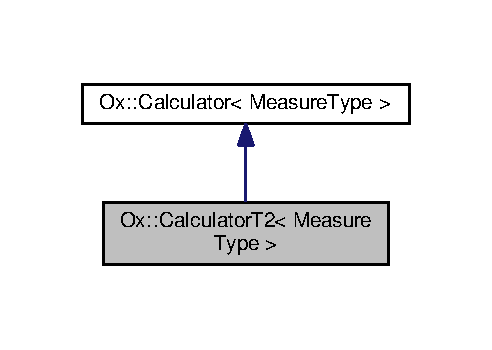
\includegraphics[width=236pt]{class_ox_1_1_calculator_t2__coll__graph}
\end{center}
\end{figure}
\subsection*{Public Member Functions}
\begin{DoxyCompactItemize}
\item 
virtual int \hyperlink{class_ox_1_1_calculator_t2_a56e2bcb27465a83dd1a1150b7fe419c8}{prepare\-To\-Calculate} ()
\item 
virtual int \hyperlink{class_ox_1_1_calculator_t2_a8afe4974f3253edea4386a87695607ae}{calculate} ()
\item 
Measure\-Type \hyperlink{class_ox_1_1_calculator_t2_ace5f0515839bdffffb3d60e4536167b6}{calculate\-R2\-Abs\-From\-Model} (int n\-Samples, const Measure\-Type $\ast$time, const Measure\-Type $\ast$signal, const Measure\-Type $\ast$parameters)
\item 
const Measure\-Type $\ast$ \hyperlink{class_ox_1_1_calculator_t2_a1f43cfb6a385e6eeb2ff8fe167ab347d}{get\-Echo\-Times} () const 
\item 
\hyperlink{class_ox_1_1_calculator_t2_a9d0d9d252c322a6db51693ef42c0bed7}{Calculator\-T2} ()
\item 
virtual \hyperlink{class_ox_1_1_calculator_t2_a0a8e02ccb647bb1faf00dbcd4f61124c}{$\sim$\-Calculator\-T2} ()
\item 
virtual \hyperlink{class_ox_1_1_calculator}{Calculator}$<$ Measure\-Type $>$ $\ast$ \hyperlink{class_ox_1_1_calculator_t2_aaec3b1e6254b67b309c9beedb54ad9e7}{new\-By\-Cloning} ()
\end{DoxyCompactItemize}
\subsection*{Additional Inherited Members}


\subsection{Detailed Description}
\subsubsection*{template$<$typename Measure\-Type$>$class Ox\-::\-Calculator\-T2$<$ Measure\-Type $>$}


\begin{DoxyTemplParams}{Template Parameters}
{\em Measure\-Type} & \\
\hline
\end{DoxyTemplParams}


\subsection{Constructor \& Destructor Documentation}
\hypertarget{class_ox_1_1_calculator_t2_a9d0d9d252c322a6db51693ef42c0bed7}{\index{Ox\-::\-Calculator\-T2@{Ox\-::\-Calculator\-T2}!Calculator\-T2@{Calculator\-T2}}
\index{Calculator\-T2@{Calculator\-T2}!Ox::CalculatorT2@{Ox\-::\-Calculator\-T2}}
\subsubsection[{Calculator\-T2}]{\setlength{\rightskip}{0pt plus 5cm}template$<$typename Measure\-Type$>$ {\bf Ox\-::\-Calculator\-T2}$<$ Measure\-Type $>$\-::{\bf Calculator\-T2} (
\begin{DoxyParamCaption}
{}
\end{DoxyParamCaption}
)\hspace{0.3cm}{\ttfamily [inline]}}}\label{class_ox_1_1_calculator_t2_a9d0d9d252c322a6db51693ef42c0bed7}
constructor \hypertarget{class_ox_1_1_calculator_t2_a0a8e02ccb647bb1faf00dbcd4f61124c}{\index{Ox\-::\-Calculator\-T2@{Ox\-::\-Calculator\-T2}!$\sim$\-Calculator\-T2@{$\sim$\-Calculator\-T2}}
\index{$\sim$\-Calculator\-T2@{$\sim$\-Calculator\-T2}!Ox::CalculatorT2@{Ox\-::\-Calculator\-T2}}
\subsubsection[{$\sim$\-Calculator\-T2}]{\setlength{\rightskip}{0pt plus 5cm}template$<$typename Measure\-Type$>$ virtual {\bf Ox\-::\-Calculator\-T2}$<$ Measure\-Type $>$\-::$\sim${\bf Calculator\-T2} (
\begin{DoxyParamCaption}
{}
\end{DoxyParamCaption}
)\hspace{0.3cm}{\ttfamily [inline]}, {\ttfamily [virtual]}}}\label{class_ox_1_1_calculator_t2_a0a8e02ccb647bb1faf00dbcd4f61124c}
destructor 

\subsection{Member Function Documentation}
\hypertarget{class_ox_1_1_calculator_t2_a8afe4974f3253edea4386a87695607ae}{\index{Ox\-::\-Calculator\-T2@{Ox\-::\-Calculator\-T2}!calculate@{calculate}}
\index{calculate@{calculate}!Ox::CalculatorT2@{Ox\-::\-Calculator\-T2}}
\subsubsection[{calculate}]{\setlength{\rightskip}{0pt plus 5cm}template$<$typename Measure\-Type $>$ int {\bf Ox\-::\-Calculator\-T2}$<$ Measure\-Type $>$\-::calculate (
\begin{DoxyParamCaption}
{}
\end{DoxyParamCaption}
)\hspace{0.3cm}{\ttfamily [virtual]}}}\label{class_ox_1_1_calculator_t2_a8afe4974f3253edea4386a87695607ae}
calling calculate\-Molli(int n\-Samples, const Measure\-Type$\ast$ inv\-Times, Measure\-Type$\ast$ signal, Measure\-Type$\ast$ signs) \begin{DoxyReturn}{Returns}
success/failure 
\end{DoxyReturn}


Implements \hyperlink{class_ox_1_1_calculator_a9638894f2ec526b68f46f02122bae0c3}{Ox\-::\-Calculator$<$ Measure\-Type $>$}.

\hypertarget{class_ox_1_1_calculator_t2_ace5f0515839bdffffb3d60e4536167b6}{\index{Ox\-::\-Calculator\-T2@{Ox\-::\-Calculator\-T2}!calculate\-R2\-Abs\-From\-Model@{calculate\-R2\-Abs\-From\-Model}}
\index{calculate\-R2\-Abs\-From\-Model@{calculate\-R2\-Abs\-From\-Model}!Ox::CalculatorT2@{Ox\-::\-Calculator\-T2}}
\subsubsection[{calculate\-R2\-Abs\-From\-Model}]{\setlength{\rightskip}{0pt plus 5cm}template$<$typename Measure\-Type $>$ Measure\-Type {\bf Ox\-::\-Calculator\-T2}$<$ Measure\-Type $>$\-::calculate\-R2\-Abs\-From\-Model (
\begin{DoxyParamCaption}
\item[{int}]{n\-Samples, }
\item[{const Measure\-Type $\ast$}]{time, }
\item[{const Measure\-Type $\ast$}]{signal, }
\item[{const Measure\-Type $\ast$}]{parameters}
\end{DoxyParamCaption}
)}}\label{class_ox_1_1_calculator_t2_ace5f0515839bdffffb3d60e4536167b6}
Calculate goodness of fit map 
\begin{DoxyParams}{Parameters}
{\em n\-Samples} & \\
\hline
{\em inv\-Times} & \\
\hline
{\em signal} & \\
\hline
{\em parameters} & \\
\hline
\end{DoxyParams}
\begin{DoxyReturn}{Returns}

\end{DoxyReturn}
\hypertarget{class_ox_1_1_calculator_t2_a1f43cfb6a385e6eeb2ff8fe167ab347d}{\index{Ox\-::\-Calculator\-T2@{Ox\-::\-Calculator\-T2}!get\-Echo\-Times@{get\-Echo\-Times}}
\index{get\-Echo\-Times@{get\-Echo\-Times}!Ox::CalculatorT2@{Ox\-::\-Calculator\-T2}}
\subsubsection[{get\-Echo\-Times}]{\setlength{\rightskip}{0pt plus 5cm}template$<$typename Measure\-Type $>$ const Measure\-Type $\ast$ {\bf Ox\-::\-Calculator\-T2}$<$ Measure\-Type $>$\-::get\-Echo\-Times (
\begin{DoxyParamCaption}
{}
\end{DoxyParamCaption}
) const\hspace{0.3cm}{\ttfamily [virtual]}}}\label{class_ox_1_1_calculator_t2_a1f43cfb6a385e6eeb2ff8fe167ab347d}
/throw exception if \-\_\-\-Echo\-Times == 0 \begin{DoxyReturn}{Returns}

\end{DoxyReturn}


Reimplemented from \hyperlink{class_ox_1_1_calculator}{Ox\-::\-Calculator$<$ Measure\-Type $>$}.

\hypertarget{class_ox_1_1_calculator_t2_aaec3b1e6254b67b309c9beedb54ad9e7}{\index{Ox\-::\-Calculator\-T2@{Ox\-::\-Calculator\-T2}!new\-By\-Cloning@{new\-By\-Cloning}}
\index{new\-By\-Cloning@{new\-By\-Cloning}!Ox::CalculatorT2@{Ox\-::\-Calculator\-T2}}
\subsubsection[{new\-By\-Cloning}]{\setlength{\rightskip}{0pt plus 5cm}template$<$typename Measure\-Type$>$ virtual {\bf Calculator}$<$Measure\-Type$>$$\ast$ {\bf Ox\-::\-Calculator\-T2}$<$ Measure\-Type $>$\-::new\-By\-Cloning (
\begin{DoxyParamCaption}
{}
\end{DoxyParamCaption}
)\hspace{0.3cm}{\ttfamily [inline]}, {\ttfamily [virtual]}}}\label{class_ox_1_1_calculator_t2_aaec3b1e6254b67b309c9beedb54ad9e7}
cloning \begin{DoxyReturn}{Returns}

\end{DoxyReturn}


Implements \hyperlink{class_ox_1_1_calculator_aaec48f39f9b0ea1b622485cf25fba484}{Ox\-::\-Calculator$<$ Measure\-Type $>$}.

\hypertarget{class_ox_1_1_calculator_t2_a56e2bcb27465a83dd1a1150b7fe419c8}{\index{Ox\-::\-Calculator\-T2@{Ox\-::\-Calculator\-T2}!prepare\-To\-Calculate@{prepare\-To\-Calculate}}
\index{prepare\-To\-Calculate@{prepare\-To\-Calculate}!Ox::CalculatorT2@{Ox\-::\-Calculator\-T2}}
\subsubsection[{prepare\-To\-Calculate}]{\setlength{\rightskip}{0pt plus 5cm}template$<$typename Measure\-Type $>$ int {\bf Ox\-::\-Calculator\-T2}$<$ Measure\-Type $>$\-::prepare\-To\-Calculate (
\begin{DoxyParamCaption}
{}
\end{DoxyParamCaption}
)\hspace{0.3cm}{\ttfamily [virtual]}}}\label{class_ox_1_1_calculator_t2_a56e2bcb27465a83dd1a1150b7fe419c8}
do all the checks and prepare to do the calculation, for example calc signal/signs and \-\_\-\-T\-R\-Raverage\-H\-B \begin{DoxyReturn}{Returns}
success/failure 
\end{DoxyReturn}


Implements \hyperlink{class_ox_1_1_calculator_a01267c4e842b35f7eacaa9aacdd7e766}{Ox\-::\-Calculator$<$ Measure\-Type $>$}.



The documentation for this class was generated from the following files\-:\begin{DoxyCompactItemize}
\item 
lib/\hyperlink{_ox_calculator_t2_8h}{Ox\-Calculator\-T2.\-h}\item 
lib/\hyperlink{_ox_calculator_t2_8hxx}{Ox\-Calculator\-T2.\-hxx}\end{DoxyCompactItemize}

\hypertarget{class_ox_1_1_factory_of_calculators}{}\section{Ox\+:\+:Factory\+Of\+Calculators$<$ T\+Y\+PE $>$ Class Template Reference}
\label{class_ox_1_1_factory_of_calculators}\index{Ox\+::\+Factory\+Of\+Calculators$<$ T\+Y\+P\+E $>$@{Ox\+::\+Factory\+Of\+Calculators$<$ T\+Y\+P\+E $>$}}
\subsection*{Static Public Member Functions}
\begin{DoxyCompactItemize}
\item 
static \hyperlink{class_ox_1_1_calculator}{Calculator}$<$ T\+Y\+PE $>$ $\ast$ {\bfseries new\+By\+Factory} (\hyperlink{class_ox_1_1_tomato_options}{Tomato\+Options}$<$ T\+Y\+PE $>$ $\ast$opts)\hypertarget{class_ox_1_1_factory_of_calculators_a43c28f519cc510bc1c8d1a86b14512b4}{}\label{class_ox_1_1_factory_of_calculators_a43c28f519cc510bc1c8d1a86b14512b4}

\item 
static void {\bfseries disp} (int parameter\+\_\+to\+\_\+map=-\/1)\hypertarget{class_ox_1_1_factory_of_calculators_a80052ba880fca49a529c839b33927b21}{}\label{class_ox_1_1_factory_of_calculators_a80052ba880fca49a529c839b33927b21}

\end{DoxyCompactItemize}


The documentation for this class was generated from the following files\+:\begin{DoxyCompactItemize}
\item 
lib/\hyperlink{_ox_factory_of_calculators_8h}{Ox\+Factory\+Of\+Calculators.\+h}\item 
lib/\hyperlink{_ox_factory_of_calculators_8hxx}{Ox\+Factory\+Of\+Calculators.\+hxx}\end{DoxyCompactItemize}

\hypertarget{class_ox_1_1_factory_of_fitters}{\section{Ox\-:\-:Factory\-Of\-Fitters$<$ T\-Y\-P\-E $>$ Class Template Reference}
\label{class_ox_1_1_factory_of_fitters}\index{Ox\-::\-Factory\-Of\-Fitters$<$ T\-Y\-P\-E $>$@{Ox\-::\-Factory\-Of\-Fitters$<$ T\-Y\-P\-E $>$}}
}
\subsection*{Static Public Member Functions}
\begin{DoxyCompactItemize}
\item 
\hypertarget{class_ox_1_1_factory_of_fitters_aeec858b4bf98eb6f7915ead00c3ede10}{static \hyperlink{class_ox_1_1_fitter}{Fitter}$<$ T\-Y\-P\-E $>$ $\ast$ {\bfseries new\-By\-Factory} (\hyperlink{struct_ox_1_1_tomato_options}{Tomato\-Options}$<$ T\-Y\-P\-E $>$ $\ast$opts)}\label{class_ox_1_1_factory_of_fitters_aeec858b4bf98eb6f7915ead00c3ede10}

\end{DoxyCompactItemize}


The documentation for this class was generated from the following file\-:\begin{DoxyCompactItemize}
\item 
app/\hyperlink{_ox_factory_of_fitters_8h}{Ox\-Factory\-Of\-Fitters.\-h}\end{DoxyCompactItemize}

\hypertarget{class_ox_1_1_factory_of_models}{\section{Ox\-:\-:Factory\-Of\-Models$<$ T\-Y\-P\-E $>$ Class Template Reference}
\label{class_ox_1_1_factory_of_models}\index{Ox\-::\-Factory\-Of\-Models$<$ T\-Y\-P\-E $>$@{Ox\-::\-Factory\-Of\-Models$<$ T\-Y\-P\-E $>$}}
}
\subsection*{Static Public Member Functions}
\begin{DoxyCompactItemize}
\item 
\hypertarget{class_ox_1_1_factory_of_models_a8aa8c31ff21f77ba4134098f68525c95}{static \hyperlink{class_ox_1_1_model}{Model}$<$ T\-Y\-P\-E $>$ $\ast$ {\bfseries new\-By\-Factory} (\hyperlink{struct_ox_1_1_tomato_options}{Tomato\-Options}$<$ T\-Y\-P\-E $>$ $\ast$opts)}\label{class_ox_1_1_factory_of_models_a8aa8c31ff21f77ba4134098f68525c95}

\item 
\hypertarget{class_ox_1_1_factory_of_models_a7f854079e81a2ef5e4e880b4a7ffb81e}{static void {\bfseries disp} (int model\-\_\-type=-\/1)}\label{class_ox_1_1_factory_of_models_a7f854079e81a2ef5e4e880b4a7ffb81e}

\end{DoxyCompactItemize}


The documentation for this class was generated from the following file\-:\begin{DoxyCompactItemize}
\item 
app/Ox\-Factory\-Of\-Models.\-h\end{DoxyCompactItemize}

\hypertarget{class_ox_1_1_factory_of_sign_calculators}{\section{Ox\-:\-:Factory\-Of\-Sign\-Calculators$<$ T\-Y\-P\-E $>$ Class Template Reference}
\label{class_ox_1_1_factory_of_sign_calculators}\index{Ox\-::\-Factory\-Of\-Sign\-Calculators$<$ T\-Y\-P\-E $>$@{Ox\-::\-Factory\-Of\-Sign\-Calculators$<$ T\-Y\-P\-E $>$}}
}
\subsection*{Static Public Member Functions}
\begin{DoxyCompactItemize}
\item 
\hypertarget{class_ox_1_1_factory_of_sign_calculators_a1241354771109d5dbd3ffb3d6ec817a3}{static \hyperlink{class_ox_1_1_sign_calculator}{Sign\-Calculator}$<$ T\-Y\-P\-E $>$ $\ast$ {\bfseries new\-By\-Factory} (\hyperlink{struct_ox_1_1_tomato_options}{Tomato\-Options}$<$ T\-Y\-P\-E $>$ $\ast$opts)}\label{class_ox_1_1_factory_of_sign_calculators_a1241354771109d5dbd3ffb3d6ec817a3}

\item 
\hypertarget{class_ox_1_1_factory_of_sign_calculators_a1230de323f020ee2f5bef7d93636c6f2}{static void {\bfseries disp} (int sign\-\_\-calc\-\_\-method=-\/1)}\label{class_ox_1_1_factory_of_sign_calculators_a1230de323f020ee2f5bef7d93636c6f2}

\end{DoxyCompactItemize}


The documentation for this class was generated from the following files\-:\begin{DoxyCompactItemize}
\item 
lib/\hyperlink{_ox_factory_of_sign_calculators_8h}{Ox\-Factory\-Of\-Sign\-Calculators.\-h}\item 
lib/\hyperlink{_ox_factory_of_sign_calculators_8hxx}{Ox\-Factory\-Of\-Sign\-Calculators.\-hxx}\end{DoxyCompactItemize}

\hypertarget{class_ox_1_1_factory_of_start_point_calculators}{\section{Ox\-:\-:Factory\-Of\-Start\-Point\-Calculators$<$ T\-Y\-P\-E $>$ Class Template Reference}
\label{class_ox_1_1_factory_of_start_point_calculators}\index{Ox\-::\-Factory\-Of\-Start\-Point\-Calculators$<$ T\-Y\-P\-E $>$@{Ox\-::\-Factory\-Of\-Start\-Point\-Calculators$<$ T\-Y\-P\-E $>$}}
}
\subsection*{Static Public Member Functions}
\begin{DoxyCompactItemize}
\item 
\hypertarget{class_ox_1_1_factory_of_start_point_calculators_a49529379f7de8796134663b95277cdb0}{static \hyperlink{class_ox_1_1_start_point_calculator}{Start\-Point\-Calculator}\\*
$<$ T\-Y\-P\-E $>$ $\ast$ {\bfseries new\-By\-Factory} (\hyperlink{struct_ox_1_1_ox_shmolli2_options}{Ox\-Shmolli2\-Options}$<$ T\-Y\-P\-E $>$ $\ast$opts)}\label{class_ox_1_1_factory_of_start_point_calculators_a49529379f7de8796134663b95277cdb0}

\end{DoxyCompactItemize}


The documentation for this class was generated from the following file\-:\begin{DoxyCompactItemize}
\item 
app/\hyperlink{_ox_factory_of_start_point_calculators_8h}{Ox\-Factory\-Of\-Start\-Point\-Calculators.\-h}\end{DoxyCompactItemize}

\hypertarget{class_ox_1_1_fitter}{}\section{Ox\+:\+:Fitter$<$ Measure\+Type $>$ Class Template Reference}
\label{class_ox_1_1_fitter}\index{Ox\+::\+Fitter$<$ Measure\+Type $>$@{Ox\+::\+Fitter$<$ Measure\+Type $>$}}


{\ttfamily \#include $<$Ox\+Fitter.\+h$>$}

\subsection*{Public Member Functions}
\begin{DoxyCompactItemize}
\item 
virtual int \hyperlink{class_ox_1_1_fitter_a8f240f0da86d06b339ab2747e87f21b9}{perform\+Fitting} ()=0
\item 
virtual const \hyperlink{class_ox_1_1_model}{Model}$<$ Measure\+Type $>$ $\ast$ {\bfseries get\+Model} () const \hypertarget{class_ox_1_1_fitter_aab3e83fef361dc2dfa855c4988af2393}{}\label{class_ox_1_1_fitter_aab3e83fef361dc2dfa855c4988af2393}

\item 
virtual Measure\+Type $\ast$ {\bfseries get\+Parameters} ()\hypertarget{class_ox_1_1_fitter_a5e87dd37738745f98d904865f6b89219}{}\label{class_ox_1_1_fitter_a5e87dd37738745f98d904865f6b89219}

\item 
virtual Measure\+Type {\bfseries get\+Mse} () const \hypertarget{class_ox_1_1_fitter_ade772dbac027c450451fc6845ce710f5}{}\label{class_ox_1_1_fitter_ade772dbac027c450451fc6845ce710f5}

\item 
virtual const Measure\+Type {\bfseries get\+X\+Tolerance} () const \hypertarget{class_ox_1_1_fitter_a21f92547f664c9b6f3fa8da4c7d16965}{}\label{class_ox_1_1_fitter_a21f92547f664c9b6f3fa8da4c7d16965}

\item 
virtual const Measure\+Type {\bfseries get\+F\+Tolerance} () const \hypertarget{class_ox_1_1_fitter_ac62bf275718aafc95b5e49d0aa9fc1ef}{}\label{class_ox_1_1_fitter_ac62bf275718aafc95b5e49d0aa9fc1ef}

\item 
virtual const bool {\bfseries get\+Use\+Gradient} () const \hypertarget{class_ox_1_1_fitter_aba3fc8ad5260390faf59e2f904ab6d6d}{}\label{class_ox_1_1_fitter_aba3fc8ad5260390faf59e2f904ab6d6d}

\item 
virtual const unsigned int {\bfseries get\+Max\+Function\+Evals} () const \hypertarget{class_ox_1_1_fitter_a04f36e075f86c6a89df833d17b9f029d}{}\label{class_ox_1_1_fitter_a04f36e075f86c6a89df833d17b9f029d}

\item 
virtual const unsigned int {\bfseries get\+Thread\+Id} () const \hypertarget{class_ox_1_1_fitter_a68e317f1c05ea2aa24f9d4803ee19215}{}\label{class_ox_1_1_fitter_a68e317f1c05ea2aa24f9d4803ee19215}

\item 
virtual const bool {\bfseries get\+Verbose} () const \hypertarget{class_ox_1_1_fitter_afeba16a2218db1f3fc646e2dde75f386}{}\label{class_ox_1_1_fitter_afeba16a2218db1f3fc646e2dde75f386}

\item 
virtual const bool {\bfseries get\+Trace} () const \hypertarget{class_ox_1_1_fitter_a9c3401372be5c8698464deb05c0f5533}{}\label{class_ox_1_1_fitter_a9c3401372be5c8698464deb05c0f5533}

\item 
virtual void {\bfseries set\+Model} (\hyperlink{class_ox_1_1_model}{Model}$<$ Measure\+Type $>$ $\ast$\+\_\+\+Model\+T1)\hypertarget{class_ox_1_1_fitter_a58bc5939283a694d4683dcc160ad4009}{}\label{class_ox_1_1_fitter_a58bc5939283a694d4683dcc160ad4009}

\item 
virtual void {\bfseries set\+Parameters} (Measure\+Type $\ast$\+\_\+\+Parameters)\hypertarget{class_ox_1_1_fitter_ab97f65c7d4d4db9bb0f5934aa0601b73}{}\label{class_ox_1_1_fitter_ab97f65c7d4d4db9bb0f5934aa0601b73}

\item 
virtual void {\bfseries set\+Mse} (Measure\+Type mse)\hypertarget{class_ox_1_1_fitter_a6a76eaeb797c09b75b9c0c3cd6ed326b}{}\label{class_ox_1_1_fitter_a6a76eaeb797c09b75b9c0c3cd6ed326b}

\item 
virtual void {\bfseries set\+X\+Tolerance} (const Measure\+Type \+\_\+\+X\+Tolerance)\hypertarget{class_ox_1_1_fitter_ad2b680ee88b12dd51538a2da865b2589}{}\label{class_ox_1_1_fitter_ad2b680ee88b12dd51538a2da865b2589}

\item 
virtual void {\bfseries set\+Use\+Gradient} (const bool \+\_\+\+Use\+Gradient)\hypertarget{class_ox_1_1_fitter_a2441247888adc90a26d779043f10c5e1}{}\label{class_ox_1_1_fitter_a2441247888adc90a26d779043f10c5e1}

\item 
virtual void {\bfseries set\+F\+Tolerance} (const Measure\+Type \+\_\+\+F\+Tolerance)\hypertarget{class_ox_1_1_fitter_aca7109a663e737c46cb29483c2276f4a}{}\label{class_ox_1_1_fitter_aca7109a663e737c46cb29483c2276f4a}

\item 
virtual void {\bfseries set\+Max\+Function\+Evals} (const unsigned int \+\_\+\+Max\+Function\+Evals)\hypertarget{class_ox_1_1_fitter_a293d2876b8b053bd637c35c3f6f3f68e}{}\label{class_ox_1_1_fitter_a293d2876b8b053bd637c35c3f6f3f68e}

\item 
virtual void {\bfseries set\+Thread\+Id} (const unsigned int \+\_\+\+Thread\+Id)\hypertarget{class_ox_1_1_fitter_aa1fc4674aa6a3e6c8567c86ec1fa90e0}{}\label{class_ox_1_1_fitter_aa1fc4674aa6a3e6c8567c86ec1fa90e0}

\item 
virtual void {\bfseries set\+Verbose} (const bool \+\_\+\+Verbose)\hypertarget{class_ox_1_1_fitter_a696da03b83fe3083f29ae4c0e2ecfc44}{}\label{class_ox_1_1_fitter_a696da03b83fe3083f29ae4c0e2ecfc44}

\item 
virtual void {\bfseries set\+Trace} (const bool \+\_\+\+Trace)\hypertarget{class_ox_1_1_fitter_a4ac0096f6bc6d733c542d28a839d32c9}{}\label{class_ox_1_1_fitter_a4ac0096f6bc6d733c542d28a839d32c9}

\item 
virtual void \hyperlink{class_ox_1_1_fitter_a783ba791c88d7208deb4004354b10022}{copy\+To\+Parameters} (const Measure\+Type $\ast$ptr\+From)
\item 
virtual void \hyperlink{class_ox_1_1_fitter_a0a9b45eb21ba174327f95a894e6331b6}{disp} ()\hypertarget{class_ox_1_1_fitter_a0a9b45eb21ba174327f95a894e6331b6}{}\label{class_ox_1_1_fitter_a0a9b45eb21ba174327f95a894e6331b6}

\begin{DoxyCompactList}\small\item\em show me your \hyperlink{class_ox_1_1_fitter}{Fitter} \end{DoxyCompactList}\item 
\hyperlink{class_ox_1_1_fitter_a7b42acb389394bc4c496990eea8b9ac9}{Fitter} ()\hypertarget{class_ox_1_1_fitter_a7b42acb389394bc4c496990eea8b9ac9}{}\label{class_ox_1_1_fitter_a7b42acb389394bc4c496990eea8b9ac9}

\begin{DoxyCompactList}\small\item\em constructor \end{DoxyCompactList}\item 
\hyperlink{class_ox_1_1_fitter_ac51130b722159f88a0dad59877b76417}{Fitter} (const \hyperlink{class_ox_1_1_fitter}{Fitter} \&old)
\item 
virtual \hyperlink{class_ox_1_1_fitter}{Fitter}$<$ Measure\+Type $>$ $\ast$ \hyperlink{class_ox_1_1_fitter_a665ec51e52ed351c9ef801acc83fbdea}{new\+By\+Cloning} ()=0
\item 
virtual \hyperlink{class_ox_1_1_fitter_ab56eef37096f6f0687d83b8d15e00d43}{$\sim$\+Fitter} ()\hypertarget{class_ox_1_1_fitter_ab56eef37096f6f0687d83b8d15e00d43}{}\label{class_ox_1_1_fitter_ab56eef37096f6f0687d83b8d15e00d43}

\begin{DoxyCompactList}\small\item\em do not forget about the virtual destructor, see \href{https://stackoverflow.com/questions/461203/when-to-use-virtual-destructors}{\tt https\+://stackoverflow.\+com/questions/461203/when-\/to-\/use-\/virtual-\/destructors} \end{DoxyCompactList}\end{DoxyCompactItemize}
\subsection*{Protected Attributes}
\begin{DoxyCompactItemize}
\item 
\hyperlink{class_ox_1_1_model}{Model}$<$ Measure\+Type $>$ $\ast$ {\bfseries \+\_\+\+Model}\hypertarget{class_ox_1_1_fitter_ae5a2d2967fb117386a4b73123f188213}{}\label{class_ox_1_1_fitter_ae5a2d2967fb117386a4b73123f188213}

\item 
Measure\+Type $\ast$ {\bfseries \+\_\+\+Parameters}\hypertarget{class_ox_1_1_fitter_a508e5654aaf79dd744ec816d95b7e33c}{}\label{class_ox_1_1_fitter_a508e5654aaf79dd744ec816d95b7e33c}

\item 
Measure\+Type {\bfseries \+\_\+\+Mse}\hypertarget{class_ox_1_1_fitter_a1c5f4e7fa0764489e30685f47fe53190}{}\label{class_ox_1_1_fitter_a1c5f4e7fa0764489e30685f47fe53190}

\item 
Measure\+Type {\bfseries \+\_\+\+X\+Tolerance}\hypertarget{class_ox_1_1_fitter_af91a5ea8fb20072277ddcd64f5537b09}{}\label{class_ox_1_1_fitter_af91a5ea8fb20072277ddcd64f5537b09}

\item 
Measure\+Type {\bfseries \+\_\+\+F\+Tolerance}\hypertarget{class_ox_1_1_fitter_a926f6cf38998f041c31b079e93bf27ab}{}\label{class_ox_1_1_fitter_a926f6cf38998f041c31b079e93bf27ab}

\item 
unsigned int {\bfseries \+\_\+\+Max\+Function\+Evals}\hypertarget{class_ox_1_1_fitter_a3be7ea1c1f19d3f4fb384474e2b1a033}{}\label{class_ox_1_1_fitter_a3be7ea1c1f19d3f4fb384474e2b1a033}

\item 
bool {\bfseries \+\_\+\+Use\+Gradient}\hypertarget{class_ox_1_1_fitter_a34c039e87d52c28b19092535a171264f}{}\label{class_ox_1_1_fitter_a34c039e87d52c28b19092535a171264f}

\item 
unsigned int {\bfseries \+\_\+\+Thread\+Id}\hypertarget{class_ox_1_1_fitter_a0d97d7a9c9fad0349484151464fefe4f}{}\label{class_ox_1_1_fitter_a0d97d7a9c9fad0349484151464fefe4f}

\item 
bool {\bfseries \+\_\+\+Verbose}\hypertarget{class_ox_1_1_fitter_a6457339f5252c85d7c92f20439544975}{}\label{class_ox_1_1_fitter_a6457339f5252c85d7c92f20439544975}

\item 
bool {\bfseries \+\_\+\+Trace}\hypertarget{class_ox_1_1_fitter_a9ba79cb05ecc670254b3e7ddafc519ab}{}\label{class_ox_1_1_fitter_a9ba79cb05ecc670254b3e7ddafc519ab}

\end{DoxyCompactItemize}


\subsection{Detailed Description}
\subsubsection*{template$<$typename Measure\+Type$>$\\*
class Ox\+::\+Fitter$<$ Measure\+Type $>$}


\begin{DoxyTemplParams}{Template Parameters}
{\em Measure\+Type} & \\
\hline
\end{DoxyTemplParams}


\subsection{Constructor \& Destructor Documentation}
\index{Ox\+::\+Fitter@{Ox\+::\+Fitter}!Fitter@{Fitter}}
\index{Fitter@{Fitter}!Ox\+::\+Fitter@{Ox\+::\+Fitter}}
\subsubsection[{\texorpdfstring{Fitter(const Fitter \&old)}{Fitter(const Fitter &old)}}]{\setlength{\rightskip}{0pt plus 5cm}template$<$typename Measure\+Type$>$ {\bf Ox\+::\+Fitter}$<$ Measure\+Type $>$\+::{\bf Fitter} (
\begin{DoxyParamCaption}
\item[{const {\bf Fitter}$<$ Measure\+Type $>$ \&}]{old}
\end{DoxyParamCaption}
)\hspace{0.3cm}{\ttfamily [inline]}}\hypertarget{class_ox_1_1_fitter_ac51130b722159f88a0dad59877b76417}{}\label{class_ox_1_1_fitter_ac51130b722159f88a0dad59877b76417}
copy constructor 
\begin{DoxyParams}{Parameters}
{\em old} & \\
\hline
\end{DoxyParams}


\subsection{Member Function Documentation}
\index{Ox\+::\+Fitter@{Ox\+::\+Fitter}!copy\+To\+Parameters@{copy\+To\+Parameters}}
\index{copy\+To\+Parameters@{copy\+To\+Parameters}!Ox\+::\+Fitter@{Ox\+::\+Fitter}}
\subsubsection[{\texorpdfstring{copy\+To\+Parameters(const Measure\+Type $\ast$ptr\+From)}{copyToParameters(const MeasureType *ptrFrom)}}]{\setlength{\rightskip}{0pt plus 5cm}template$<$typename Measure\+Type$>$ virtual void {\bf Ox\+::\+Fitter}$<$ Measure\+Type $>$\+::copy\+To\+Parameters (
\begin{DoxyParamCaption}
\item[{const Measure\+Type $\ast$}]{ptr\+From}
\end{DoxyParamCaption}
)\hspace{0.3cm}{\ttfamily [inline]}, {\ttfamily [virtual]}}\hypertarget{class_ox_1_1_fitter_a783ba791c88d7208deb4004354b10022}{}\label{class_ox_1_1_fitter_a783ba791c88d7208deb4004354b10022}
copy from ptr\+From to the parameters. Parameters have to be allocated first 
\begin{DoxyParams}{Parameters}
{\em ptr\+From} & \\
\hline
\end{DoxyParams}
\index{Ox\+::\+Fitter@{Ox\+::\+Fitter}!new\+By\+Cloning@{new\+By\+Cloning}}
\index{new\+By\+Cloning@{new\+By\+Cloning}!Ox\+::\+Fitter@{Ox\+::\+Fitter}}
\subsubsection[{\texorpdfstring{new\+By\+Cloning()=0}{newByCloning()=0}}]{\setlength{\rightskip}{0pt plus 5cm}template$<$typename Measure\+Type$>$ virtual {\bf Fitter}$<$Measure\+Type$>$$\ast$ {\bf Ox\+::\+Fitter}$<$ Measure\+Type $>$\+::new\+By\+Cloning (
\begin{DoxyParamCaption}
{}
\end{DoxyParamCaption}
)\hspace{0.3cm}{\ttfamily [pure virtual]}}\hypertarget{class_ox_1_1_fitter_a665ec51e52ed351c9ef801acc83fbdea}{}\label{class_ox_1_1_fitter_a665ec51e52ed351c9ef801acc83fbdea}
cloning \begin{DoxyReturn}{Returns}

\end{DoxyReturn}
\index{Ox\+::\+Fitter@{Ox\+::\+Fitter}!perform\+Fitting@{perform\+Fitting}}
\index{perform\+Fitting@{perform\+Fitting}!Ox\+::\+Fitter@{Ox\+::\+Fitter}}
\subsubsection[{\texorpdfstring{perform\+Fitting()=0}{performFitting()=0}}]{\setlength{\rightskip}{0pt plus 5cm}template$<$typename Measure\+Type$>$ virtual int {\bf Ox\+::\+Fitter}$<$ Measure\+Type $>$\+::perform\+Fitting (
\begin{DoxyParamCaption}
{}
\end{DoxyParamCaption}
)\hspace{0.3cm}{\ttfamily [pure virtual]}}\hypertarget{class_ox_1_1_fitter_a8f240f0da86d06b339ab2747e87f21b9}{}\label{class_ox_1_1_fitter_a8f240f0da86d06b339ab2747e87f21b9}
the most important function of this class \begin{DoxyReturn}{Returns}
success/failure 
\end{DoxyReturn}


The documentation for this class was generated from the following file\+:\begin{DoxyCompactItemize}
\item 
lib/\hyperlink{_ox_fitter_8h}{Ox\+Fitter.\+h}\end{DoxyCompactItemize}

\hypertarget{class_ox_1_1_image_calculator_t1}{\section{Ox\-:\-:Image\-Calculator\-T1$<$ Measure\-Type $>$ Class Template Reference}
\label{class_ox_1_1_image_calculator_t1}\index{Ox\-::\-Image\-Calculator\-T1$<$ Measure\-Type $>$@{Ox\-::\-Image\-Calculator\-T1$<$ Measure\-Type $>$}}
}
\subsection*{Public Member Functions}
\begin{DoxyCompactItemize}
\item 
\hypertarget{class_ox_1_1_image_calculator_t1_af554bf4191ef1d52469e5bb2fa832a57}{void {\bfseries set\-Use\-Threads} (bool \-\_\-use\-Threads)}\label{class_ox_1_1_image_calculator_t1_af554bf4191ef1d52469e5bb2fa832a57}

\item 
\hypertarget{class_ox_1_1_image_calculator_t1_aea2ffd0ea8668a198c8142a21c1eef4f}{void {\bfseries set\-N\-Cols} (int \-\_\-n\-Cols)}\label{class_ox_1_1_image_calculator_t1_aea2ffd0ea8668a198c8142a21c1eef4f}

\item 
\hypertarget{class_ox_1_1_image_calculator_t1_ab4cbe03b2105cc5e5d61432d3c320ab3}{void {\bfseries set\-N\-Rows} (int \-\_\-n\-Rows)}\label{class_ox_1_1_image_calculator_t1_ab4cbe03b2105cc5e5d61432d3c320ab3}

\item 
\hypertarget{class_ox_1_1_image_calculator_t1_a35729c3ccb7f4e3426a16682cecdb8a1}{void {\bfseries set\-N\-Samples} (int \-\_\-n\-Samples)}\label{class_ox_1_1_image_calculator_t1_a35729c3ccb7f4e3426a16682cecdb8a1}

\item 
\hypertarget{class_ox_1_1_image_calculator_t1_a92cbd8b336a8aaac7c7b9e5b52968454}{void {\bfseries set\-Inv\-Times} (Measure\-Type $\ast$\-\_\-inv\-Times)}\label{class_ox_1_1_image_calculator_t1_a92cbd8b336a8aaac7c7b9e5b52968454}

\item 
\hypertarget{class_ox_1_1_image_calculator_t1_a5193dd7849ec11b2173cb94fb0bcd74b}{void {\bfseries set\-Image\-Mag} (Measure\-Type $\ast$\-\_\-image\-Mag)}\label{class_ox_1_1_image_calculator_t1_a5193dd7849ec11b2173cb94fb0bcd74b}

\item 
\hypertarget{class_ox_1_1_image_calculator_t1_a4506dab7d6ad85807b68ad4b1ab7fb85}{void {\bfseries set\-Image\-Pha} (Measure\-Type $\ast$\-\_\-image\-Pha)}\label{class_ox_1_1_image_calculator_t1_a4506dab7d6ad85807b68ad4b1ab7fb85}

\item 
\hypertarget{class_ox_1_1_image_calculator_t1_a57aa44a0e067f5747dc017be41f15d78}{void {\bfseries set\-Image\-Results} (Measure\-Type $\ast$\-\_\-image\-Results)}\label{class_ox_1_1_image_calculator_t1_a57aa44a0e067f5747dc017be41f15d78}

\item 
\hypertarget{class_ox_1_1_image_calculator_t1_aedd4a349b189cee112c8637757c733c7}{void {\bfseries set\-Calculator\-T1} (\hyperlink{class_ox_1_1_calculator}{Calculator}$<$ Measure\-Type $>$ $\ast$\-\_\-calculator\-T1)}\label{class_ox_1_1_image_calculator_t1_aedd4a349b189cee112c8637757c733c7}

\item 
\hypertarget{class_ox_1_1_image_calculator_t1_ab8670346a47b573558357787b64dc94d}{Measure\-Type $\ast$ {\bfseries get\-Image\-Results} () const }\label{class_ox_1_1_image_calculator_t1_ab8670346a47b573558357787b64dc94d}

\item 
\hypertarget{class_ox_1_1_image_calculator_t1_ad97c2f2b08a7004815445027523f97ed}{virtual int {\bfseries calculate} ()}\label{class_ox_1_1_image_calculator_t1_ad97c2f2b08a7004815445027523f97ed}

\item 
\hypertarget{class_ox_1_1_image_calculator_t1_a3ff9a9627bae210326cfbeebea097cb8}{virtual int {\bfseries calculate\-One\-Thread} (int pos\-Start, int pos\-Stop)}\label{class_ox_1_1_image_calculator_t1_a3ff9a9627bae210326cfbeebea097cb8}

\end{DoxyCompactItemize}
\subsection*{Protected Attributes}
\begin{DoxyCompactItemize}
\item 
\hypertarget{class_ox_1_1_image_calculator_t1_af5f6e72b63b78a87a3723f4f2d71068f}{bool {\bfseries \-\_\-use\-Threads}}\label{class_ox_1_1_image_calculator_t1_af5f6e72b63b78a87a3723f4f2d71068f}

\item 
\hypertarget{class_ox_1_1_image_calculator_t1_a02ee85ff0ffd7cb5b1de9357ab23ce56}{int {\bfseries \-\_\-n\-Cols}}\label{class_ox_1_1_image_calculator_t1_a02ee85ff0ffd7cb5b1de9357ab23ce56}

\item 
\hypertarget{class_ox_1_1_image_calculator_t1_ab3db79a49b848f1a145e6fcbb9c29766}{int {\bfseries \-\_\-n\-Rows}}\label{class_ox_1_1_image_calculator_t1_ab3db79a49b848f1a145e6fcbb9c29766}

\item 
\hypertarget{class_ox_1_1_image_calculator_t1_af5655b9262c2634cc8b4ce0465682b0e}{int {\bfseries \-\_\-n\-Samples}}\label{class_ox_1_1_image_calculator_t1_af5655b9262c2634cc8b4ce0465682b0e}

\item 
\hypertarget{class_ox_1_1_image_calculator_t1_a6bc67b8020a51ecd2defd7ede1954b52}{Measure\-Type $\ast$ {\bfseries \-\_\-inv\-Times}}\label{class_ox_1_1_image_calculator_t1_a6bc67b8020a51ecd2defd7ede1954b52}

\item 
\hypertarget{class_ox_1_1_image_calculator_t1_ab43aaec5a7bae1246c96f366498c2130}{Measure\-Type $\ast$ {\bfseries \-\_\-image\-Mag}}\label{class_ox_1_1_image_calculator_t1_ab43aaec5a7bae1246c96f366498c2130}

\item 
\hypertarget{class_ox_1_1_image_calculator_t1_af804d044be29f0b554c68992d77f22ba}{Measure\-Type $\ast$ {\bfseries \-\_\-image\-Pha}}\label{class_ox_1_1_image_calculator_t1_af804d044be29f0b554c68992d77f22ba}

\item 
\hypertarget{class_ox_1_1_image_calculator_t1_a62bb966f944eae07d9873db02487f850}{Measure\-Type $\ast$ {\bfseries \-\_\-image\-Results}}\label{class_ox_1_1_image_calculator_t1_a62bb966f944eae07d9873db02487f850}

\item 
\hypertarget{class_ox_1_1_image_calculator_t1_a35e200233fd8e1ecdd88c8a74ae4c1d0}{Measure\-Type {\bfseries phase\-Range}}\label{class_ox_1_1_image_calculator_t1_a35e200233fd8e1ecdd88c8a74ae4c1d0}

\item 
\hypertarget{class_ox_1_1_image_calculator_t1_a1ba7f99a15c36c734abe8253cd0de4d5}{\hyperlink{class_ox_1_1_calculator}{Calculator}$<$ Measure\-Type $>$ $\ast$ {\bfseries \-\_\-calculator\-T1}}\label{class_ox_1_1_image_calculator_t1_a1ba7f99a15c36c734abe8253cd0de4d5}

\end{DoxyCompactItemize}


The documentation for this class was generated from the following files\-:\begin{DoxyCompactItemize}
\item 
lib/Ox\-Image\-Calculator\-T1.\-h\item 
lib/Ox\-Image\-Calculator\-T1.\-hxx\end{DoxyCompactItemize}

\hypertarget{class_k_w_util}{\section{K\-W\-Util Class Reference}
\label{class_k_w_util}\index{K\-W\-Util@{K\-W\-Util}}
}
\subsection*{Static Public Member Functions}
\begin{DoxyCompactItemize}
\item 
\hypertarget{class_k_w_util_a5d14be8edc626d6b30b31c8d85c64d00}{{\footnotesize template$<$typename T\-Y\-P\-E $>$ }\\static void {\bfseries print\-K\-W} (bool do\-Print, char $\ast$fmt,...)}\label{class_k_w_util_a5d14be8edc626d6b30b31c8d85c64d00}

\item 
\hypertarget{class_k_w_util_a74cbba48bf115ff4ddb90e4c8abfaaac}{{\footnotesize template$<$typename T\-Y\-P\-E1 , typename T\-Y\-P\-E2 $>$ }\\static void {\bfseries copy\-Array\-To\-Array} (int n\-Samples, T\-Y\-P\-E1 $\ast$array\-To, const T\-Y\-P\-E2 $\ast$array\-From)}\label{class_k_w_util_a74cbba48bf115ff4ddb90e4c8abfaaac}

\item 
{\footnotesize template$<$typename T\-Y\-P\-E $>$ }\\static void \hyperlink{class_k_w_util_acc956bb7cbedc39fbca11a6414b66dac}{print\-Vector} (const std\-::string \&name, const std\-::vector$<$ T\-Y\-P\-E $>$ vector)
\item 
{\footnotesize template$<$typename T\-Y\-P\-E $>$ }\\static void \hyperlink{class_k_w_util_aec00dd2420ac8d850284db70c71c1c16}{print\-Vector\-Newline} (const std\-::string \&name, const std\-::vector$<$ T\-Y\-P\-E $>$ vector)
\item 
\hypertarget{class_k_w_util_a9a809d578ed4b3647b7a92a8ee349a0e}{{\footnotesize template$<$typename T\-Y\-P\-E $>$ }\\static void {\bfseries print\-Array} (int n\-Samples, const T\-Y\-P\-E $\ast$myarray)}\label{class_k_w_util_a9a809d578ed4b3647b7a92a8ee349a0e}

\item 
\hypertarget{class_k_w_util_a43228ea0afd7071af2d990ee550472e0}{{\footnotesize template$<$typename T\-Y\-P\-E $>$ }\\static void {\bfseries print\-Array} (int n\-Samples, const T\-Y\-P\-E $\ast$myarray, int width)}\label{class_k_w_util_a43228ea0afd7071af2d990ee550472e0}

\item 
\hypertarget{class_k_w_util_aa537bb86732154b9ad1317e851afccfd}{{\footnotesize template$<$typename T\-Y\-P\-E $>$ }\\static void {\bfseries print\-Array} (int n\-Samples, const T\-Y\-P\-E $\ast$myarray, char $\ast$text)}\label{class_k_w_util_aa537bb86732154b9ad1317e851afccfd}

\item 
\hypertarget{class_k_w_util_a551666cf04781258441f4d5a77c6a7d8}{{\footnotesize template$<$typename T\-Y\-P\-E $>$ }\\static void {\bfseries print\-Array} (bool do\-Print, int n\-Samples, const T\-Y\-P\-E $\ast$myarray)}\label{class_k_w_util_a551666cf04781258441f4d5a77c6a7d8}

\item 
\hypertarget{class_k_w_util_a5eafacfaa0ea74867d2b37cf22558644}{{\footnotesize template$<$typename T\-Y\-P\-E $>$ }\\static void {\bfseries print\-Array} (bool do\-Print, int n\-Samples, const T\-Y\-P\-E $\ast$myarray, char $\ast$text)}\label{class_k_w_util_a5eafacfaa0ea74867d2b37cf22558644}

\item 
\hypertarget{class_k_w_util_a0d00bcaaee4bf9fe1ea3f28c39db766d}{{\footnotesize template$<$typename T\-Y\-P\-E $>$ }\\static void {\bfseries print\-Array2\-D} (int n\-Rows, int n\-Cols, T\-Y\-P\-E $\ast$$\ast$myarray)}\label{class_k_w_util_a0d00bcaaee4bf9fe1ea3f28c39db766d}

\item 
\hypertarget{class_k_w_util_a8ca8f9d0826b637aee5285af196431a0}{{\footnotesize template$<$typename T\-Y\-P\-E $>$ }\\static void {\bfseries print\-Array2\-D} (int n\-Rows, int n\-Cols, T\-Y\-P\-E $\ast$$\ast$myarray, char $\ast$text)}\label{class_k_w_util_a8ca8f9d0826b637aee5285af196431a0}

\item 
\hypertarget{class_k_w_util_a2907060d81976090c40829107159666d}{{\footnotesize template$<$typename T\-Y\-P\-E $>$ }\\static void {\bfseries print\-Array2\-D} (bool do\-Print, int n\-Rows, int n\-Cols, T\-Y\-P\-E $\ast$$\ast$myarray)}\label{class_k_w_util_a2907060d81976090c40829107159666d}

\item 
\hypertarget{class_k_w_util_a59aabe5a32605da8367ca84c3ad3a0ab}{{\footnotesize template$<$typename T\-Y\-P\-E $>$ }\\static void {\bfseries print\-Array2\-D} (bool do\-Print, int n\-Rows, int n\-Cols, T\-Y\-P\-E $\ast$$\ast$myarray, char $\ast$text)}\label{class_k_w_util_a59aabe5a32605da8367ca84c3ad3a0ab}

\item 
\hypertarget{class_k_w_util_aaffd937290f71df67551a6f2a00e1660}{{\footnotesize template$<$typename T\-Y\-P\-E $>$ }\\static void {\bfseries print\-Std\-Vector} (const std\-::vector$<$ T\-Y\-P\-E $>$ myvector)}\label{class_k_w_util_aaffd937290f71df67551a6f2a00e1660}

\item 
\hypertarget{class_k_w_util_a8d69c11c8b97c2bc5aee5449ece9b11d}{{\footnotesize template$<$typename T\-Y\-P\-E $>$ }\\static void {\bfseries print\-Std\-Vector} (const std\-::vector$<$ T\-Y\-P\-E $>$ myvector, char $\ast$text)}\label{class_k_w_util_a8d69c11c8b97c2bc5aee5449ece9b11d}

\item 
\hypertarget{class_k_w_util_a684d6abf0326e8d495f709c2b1d82ea2}{{\footnotesize template$<$typename T\-Y\-P\-E $>$ }\\static void {\bfseries print\-Std\-Vector} (bool do\-Print, const std\-::vector$<$ T\-Y\-P\-E $>$ myvector)}\label{class_k_w_util_a684d6abf0326e8d495f709c2b1d82ea2}

\item 
\hypertarget{class_k_w_util_ac17252f672282e2f60e76d594ed2d8f7}{{\footnotesize template$<$typename T\-Y\-P\-E $>$ }\\static void {\bfseries print\-Std\-Vector} (bool do\-Print, const std\-::vector$<$ T\-Y\-P\-E $>$ myvector, char $\ast$text)}\label{class_k_w_util_ac17252f672282e2f60e76d594ed2d8f7}

\item 
\hypertarget{class_k_w_util_a6ed5d213169247c4b3fe3ed2fb96dd88}{{\footnotesize template$<$typename T\-Y\-P\-E $>$ }\\static void {\bfseries swap} (T\-Y\-P\-E \&a, T\-Y\-P\-E \&b)}\label{class_k_w_util_a6ed5d213169247c4b3fe3ed2fb96dd88}

\item 
\hypertarget{class_k_w_util_a707d699ad01c87ba21e06fe28de85712}{{\footnotesize template$<$typename T\-Y\-P\-E $>$ }\\static T\-Y\-P\-E {\bfseries max} (T\-Y\-P\-E a, T\-Y\-P\-E b)}\label{class_k_w_util_a707d699ad01c87ba21e06fe28de85712}

\item 
\hypertarget{class_k_w_util_af1b3640361810ba75435a850d73a2413}{{\footnotesize template$<$typename T\-Y\-P\-E $>$ }\\static T\-Y\-P\-E {\bfseries min} (T\-Y\-P\-E a, T\-Y\-P\-E b)}\label{class_k_w_util_af1b3640361810ba75435a850d73a2413}

\item 
\hypertarget{class_k_w_util_abe27306f912197863466e7c68d3c66fb}{{\footnotesize template$<$typename T\-Y\-P\-E $>$ }\\static T\-Y\-P\-E {\bfseries calc\-Sum\-Array} (int n\-Samples, const T\-Y\-P\-E $\ast$myarray)}\label{class_k_w_util_abe27306f912197863466e7c68d3c66fb}

\item 
\hypertarget{class_k_w_util_ad9cb19db7d541d5ca5a60c6a28b922e1}{{\footnotesize template$<$typename T\-Y\-P\-E $>$ }\\static double {\bfseries calc\-Mean\-Array} (int n\-Samples, const T\-Y\-P\-E $\ast$myarray)}\label{class_k_w_util_ad9cb19db7d541d5ca5a60c6a28b922e1}

\item 
\hypertarget{class_k_w_util_a6c10285ae2d87ccda6ddaa18c81dea39}{{\footnotesize template$<$typename T\-Y\-P\-E $>$ }\\static double {\bfseries calc\-Median\-Array} (int n\-Samples, const T\-Y\-P\-E $\ast$myarray)}\label{class_k_w_util_a6c10285ae2d87ccda6ddaa18c81dea39}

\item 
\hypertarget{class_k_w_util_ad9d38c641f6b227be4418acf404170d4}{{\footnotesize template$<$typename T\-Y\-P\-E $>$ }\\static double {\bfseries calc\-Standard\-Deviation\-Array} (int n\-Samples, const T\-Y\-P\-E $\ast$myarray)}\label{class_k_w_util_ad9d38c641f6b227be4418acf404170d4}

\item 
\hypertarget{class_k_w_util_ae26dd38b1c5c823fa37129520bb4cc47}{{\footnotesize template$<$typename T\-Y\-P\-E $>$ }\\static double {\bfseries calc\-R2ss} (int n\-Samples, const T\-Y\-P\-E $\ast$fitted, const T\-Y\-P\-E $\ast$ysignal)}\label{class_k_w_util_ae26dd38b1c5c823fa37129520bb4cc47}

\item 
\hypertarget{class_k_w_util_a9eecfdafa3ae5e493830181fa7ea8fa3}{{\footnotesize template$<$typename T\-Y\-P\-E $>$ }\\static double {\bfseries calc\-R2cor} (int n\-Samples, const T\-Y\-P\-E $\ast$fitted, const T\-Y\-P\-E $\ast$ysignal)}\label{class_k_w_util_a9eecfdafa3ae5e493830181fa7ea8fa3}

\item 
\hypertarget{class_k_w_util_ac7633e5346a8b4ad6b2d1d960eb22fc9}{{\footnotesize template$<$typename T\-Y\-P\-E $>$ }\\static double {\bfseries S\-K\-P\-Lin\-Reg} (const T\-Y\-P\-E $\ast$datax, const T\-Y\-P\-E $\ast$datay, int n\-Samples, T\-Y\-P\-E \&rslope, T\-Y\-P\-E \&roffset)}\label{class_k_w_util_ac7633e5346a8b4ad6b2d1d960eb22fc9}

\item 
\hypertarget{class_k_w_util_adea3028ddaac44e13ab60460b0e50452}{{\footnotesize template$<$typename T\-Y\-P\-E $>$ }\\static void {\bfseries S\-K\-Psort} (int n\-Samples, const T\-Y\-P\-E $\ast$myarray, int $\ast$index)}\label{class_k_w_util_adea3028ddaac44e13ab60460b0e50452}

\item 
\hypertarget{class_k_w_util_aacc2b444dd10145dea4367714527efa9}{{\footnotesize template$<$typename T\-Y\-P\-E $>$ }\\static void {\bfseries quick\-Sort} (int n\-Samples, T\-Y\-P\-E $\ast$myarray)}\label{class_k_w_util_aacc2b444dd10145dea4367714527efa9}

\item 
\hypertarget{class_k_w_util_aba1906d9b0de1262e0ce837b15e8401f}{{\footnotesize template$<$typename T\-Y\-P\-E $>$ }\\static void {\bfseries quick\-Sort\-Index} (int n\-Samples, T\-Y\-P\-E $\ast$myarray, int $\ast$index\-Array)}\label{class_k_w_util_aba1906d9b0de1262e0ce837b15e8401f}

\item 
\hypertarget{class_k_w_util_a2e55b0bcf1bbf1155654b748a7064cbf}{{\footnotesize template$<$typename T\-Y\-P\-E $>$ }\\static T\-Y\-P\-E {\bfseries get\-Chi\-Sqrt} (T\-Y\-P\-E last\-F\-Value, int n\-Samples)}\label{class_k_w_util_a2e55b0bcf1bbf1155654b748a7064cbf}

\item 
{\footnotesize template$<$typename T\-Y\-P\-E $>$ }\\static int \hyperlink{class_k_w_util_a80504801c382f1ac367bcf0787fb18c2}{calc\-Matrix\-Inverse3x3} (const T\-Y\-P\-E $\ast$matrix, T\-Y\-P\-E $\ast$matrix\-Inverse)
\item 
\hypertarget{class_k_w_util_a6401111c5ce49eb97e1c79bae84b3868}{{\footnotesize template$<$typename T\-Y\-P\-E $>$ }\\static T\-Y\-P\-E {\bfseries M\-O\-L\-L\-I\-\_\-min} (T\-Y\-P\-E a\mbox{[}$\,$\mbox{]}, int n, int $\ast$indm)}\label{class_k_w_util_a6401111c5ce49eb97e1c79bae84b3868}

\item 
\hypertarget{class_k_w_util_af0fee5e9d89e7c029c346804480d5832}{{\footnotesize template$<$typename T\-Y\-P\-E $>$ }\\static T\-Y\-P\-E {\bfseries M\-O\-L\-L\-I\-\_\-max} (T\-Y\-P\-E a\mbox{[}$\,$\mbox{]}, int n, int $\ast$indm)}\label{class_k_w_util_af0fee5e9d89e7c029c346804480d5832}

\item 
\hypertarget{class_k_w_util_a10aaa83c83c801ef07c95a29e1acdc4e}{{\footnotesize template$<$typename T\-Y\-P\-E $>$ }\\static std\-::string {\bfseries Number\-To\-String} (T\-Y\-P\-E Number)}\label{class_k_w_util_a10aaa83c83c801ef07c95a29e1acdc4e}

\item 
\hypertarget{class_k_w_util_adea4c36750f518d1f2c90af14742a0f6}{{\footnotesize template$<$typename T\-Y\-P\-E $>$ }\\static T\-Y\-P\-E {\bfseries String\-To\-Number} (const std\-::string \&Text)}\label{class_k_w_util_adea4c36750f518d1f2c90af14742a0f6}

\item 
\hypertarget{class_k_w_util_a21813a6377e55fa15c70f64afb2feb51}{{\footnotesize template$<$typename T\-Y\-P\-E $>$ }\\static T\-Y\-P\-E {\bfseries dicom\-Time2\-Seconds} (std\-::string dicom\-Time\-String)}\label{class_k_w_util_a21813a6377e55fa15c70f64afb2feb51}

\item 
\hypertarget{class_k_w_util_a498350d10204849240a945ea682ecc98}{{\footnotesize template$<$typename T\-Y\-P\-E $>$ }\\static std\-::vector$<$ int $>$ {\bfseries bounds} (int parts, int mem)}\label{class_k_w_util_a498350d10204849240a945ea682ecc98}

\item 
\hypertarget{class_k_w_util_a19d7a4b4320a3b9d8ff06e4d296e2893}{static std\-::string {\bfseries Path\-Separator} ()}\label{class_k_w_util_a19d7a4b4320a3b9d8ff06e4d296e2893}

\item 
\hypertarget{class_k_w_util_afe6ad66b5fe06a8b42918634076ab056}{static void {\bfseries split\-Filename} (const std\-::string \&str, std\-::string \&path, std\-::string \&file)}\label{class_k_w_util_afe6ad66b5fe06a8b42918634076ab056}

\item 
\hypertarget{class_k_w_util_a70a639cebc8982645a9ba44f73b93d85}{static std\-::vector$<$ std\-::string $>$ {\bfseries read\-File} (const std\-::string file\-Path)}\label{class_k_w_util_a70a639cebc8982645a9ba44f73b93d85}

\end{DoxyCompactItemize}


\subsection{Member Function Documentation}
\hypertarget{class_k_w_util_a80504801c382f1ac367bcf0787fb18c2}{\index{K\-W\-Util@{K\-W\-Util}!calc\-Matrix\-Inverse3x3@{calc\-Matrix\-Inverse3x3}}
\index{calc\-Matrix\-Inverse3x3@{calc\-Matrix\-Inverse3x3}!KWUtil@{K\-W\-Util}}
\subsubsection[{calc\-Matrix\-Inverse3x3}]{\setlength{\rightskip}{0pt plus 5cm}template$<$typename T\-Y\-P\-E $>$ int K\-W\-Util\-::calc\-Matrix\-Inverse3x3 (
\begin{DoxyParamCaption}
\item[{const T\-Y\-P\-E $\ast$}]{matrix, }
\item[{T\-Y\-P\-E $\ast$}]{matrix\-Inverse}
\end{DoxyParamCaption}
)\hspace{0.3cm}{\ttfamily [static]}}}\label{class_k_w_util_a80504801c382f1ac367bcf0787fb18c2}

\begin{DoxyTemplParams}{Template Parameters}
{\em T\-Y\-P\-E} & \\
\hline
\end{DoxyTemplParams}

\begin{DoxyParams}{Parameters}
{\em matrix} & -\/ pointer to array with indices \mbox{[}0 1 2; 3 4 5; 6 7 8\mbox{]} \\
\hline
{\em matrix\-Inverse} & -\/ pointer to with indices \mbox{[}0 1 2; 3 4 5; 6 7 8\mbox{]}. Fills the inverse matix if determinant != 0 or zero matrix if det == 0 \\
\hline
\end{DoxyParams}
\begin{DoxyReturn}{Returns}
0 if success, 1 if det == 0 
\end{DoxyReturn}
\hypertarget{class_k_w_util_acc956bb7cbedc39fbca11a6414b66dac}{\index{K\-W\-Util@{K\-W\-Util}!print\-Vector@{print\-Vector}}
\index{print\-Vector@{print\-Vector}!KWUtil@{K\-W\-Util}}
\subsubsection[{print\-Vector}]{\setlength{\rightskip}{0pt plus 5cm}template$<$typename T\-Y\-P\-E $>$ void K\-W\-Util\-::print\-Vector (
\begin{DoxyParamCaption}
\item[{const std\-::string \&}]{name, }
\item[{const std\-::vector$<$ T\-Y\-P\-E $>$}]{vector}
\end{DoxyParamCaption}
)\hspace{0.3cm}{\ttfamily [static]}}}\label{class_k_w_util_acc956bb7cbedc39fbca11a6414b66dac}
print\-Vector 
\begin{DoxyTemplParams}{Template Parameters}
{\em T\-Y\-P\-E} & \\
\hline
\end{DoxyTemplParams}

\begin{DoxyParams}{Parameters}
{\em name} & \\
\hline
{\em vector} & \\
\hline
\end{DoxyParams}
\hypertarget{class_k_w_util_aec00dd2420ac8d850284db70c71c1c16}{\index{K\-W\-Util@{K\-W\-Util}!print\-Vector\-Newline@{print\-Vector\-Newline}}
\index{print\-Vector\-Newline@{print\-Vector\-Newline}!KWUtil@{K\-W\-Util}}
\subsubsection[{print\-Vector\-Newline}]{\setlength{\rightskip}{0pt plus 5cm}template$<$typename T\-Y\-P\-E $>$ void K\-W\-Util\-::print\-Vector\-Newline (
\begin{DoxyParamCaption}
\item[{const std\-::string \&}]{name, }
\item[{const std\-::vector$<$ T\-Y\-P\-E $>$}]{vector}
\end{DoxyParamCaption}
)\hspace{0.3cm}{\ttfamily [static]}}}\label{class_k_w_util_aec00dd2420ac8d850284db70c71c1c16}
print\-Vectorn with newlines after every element 
\begin{DoxyTemplParams}{Template Parameters}
{\em T\-Y\-P\-E} & \\
\hline
\end{DoxyTemplParams}

\begin{DoxyParams}{Parameters}
{\em name} & \\
\hline
{\em vector} & \\
\hline
\end{DoxyParams}


The documentation for this class was generated from the following files\-:\begin{DoxyCompactItemize}
\item 
lib/K\-W\-Util.\-h\item 
lib/K\-W\-Util.\-hxx\end{DoxyCompactItemize}

\hypertarget{class_ox_1_1_model}{}\section{Ox\+:\+:Model$<$ Measure\+Type $>$ Class Template Reference}
\label{class_ox_1_1_model}\index{Ox\+::\+Model$<$ Measure\+Type $>$@{Ox\+::\+Model$<$ Measure\+Type $>$}}


Container for a model function, cost function and Least-\/\+Squares function. And derivatives.  




{\ttfamily \#include $<$Ox\+Model.\+h$>$}



Inheritance diagram for Ox\+:\+:Model$<$ Measure\+Type $>$\+:
\nopagebreak
\begin{figure}[H]
\begin{center}
\leavevmode
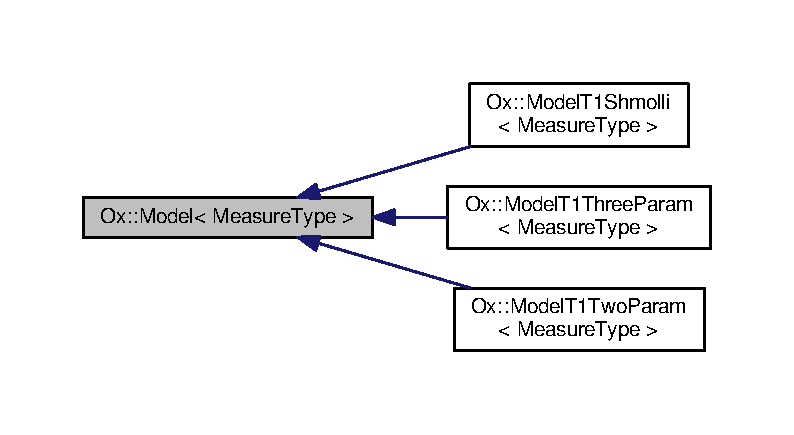
\includegraphics[width=350pt]{class_ox_1_1_model__inherit__graph}
\end{center}
\end{figure}
\subsection*{Public Member Functions}
\begin{DoxyCompactItemize}
\item 
virtual Measure\+Type \hyperlink{class_ox_1_1_model_ae3a3f5bfeefd8a8c0c012e1761eac1f5}{calc\+Model\+Value} (const Measure\+Type $\ast$parameters, Measure\+Type time)=0
\item 
virtual void \hyperlink{class_ox_1_1_model_a17e0ef71135350d4f61bef2a097fb586}{calc\+L\+S\+Residuals} (const Measure\+Type $\ast$parameters, Measure\+Type $\ast$residuals)=0
\item 
virtual Measure\+Type \hyperlink{class_ox_1_1_model_aa5997cea7114d0e323e79956adb13ba4}{calc\+Cost\+Value} (const Measure\+Type $\ast$parameters)=0
\item 
virtual void \hyperlink{class_ox_1_1_model_a274f0efdbbc364e82bba7470f933eecd}{calc\+Cost\+Derivative} (const Measure\+Type $\ast$parameters, Measure\+Type $\ast$derivative)=0
\item 
virtual void \hyperlink{class_ox_1_1_model_a4cadb65b8416b4b30e91bf6db00737f3}{calc\+L\+S\+Jacobian} (const Measure\+Type $\ast$parameters, Measure\+Type $\ast$jacobian)=0
\item 
virtual int {\bfseries get\+N\+Samples} ()\hypertarget{class_ox_1_1_model_a29715e78ec12b91c56df85fc0f782ea7}{}\label{class_ox_1_1_model_a29715e78ec12b91c56df85fc0f782ea7}

\item 
virtual const Measure\+Type $\ast$ {\bfseries get\+Inv\+Times} () const \hypertarget{class_ox_1_1_model_a7c7497927d9aa7f0c3aa5933e4a7ff7d}{}\label{class_ox_1_1_model_a7c7497927d9aa7f0c3aa5933e4a7ff7d}

\item 
virtual const Measure\+Type $\ast$ {\bfseries get\+Echo\+Times} () const \hypertarget{class_ox_1_1_model_a1606369f7a57a69c9944a54a135bc1f4}{}\label{class_ox_1_1_model_a1606369f7a57a69c9944a54a135bc1f4}

\item 
virtual const Measure\+Type $\ast$ {\bfseries get\+Rep\+Times} () const \hypertarget{class_ox_1_1_model_ad1ecd4e858e0a5386a27505ec78135c5}{}\label{class_ox_1_1_model_ad1ecd4e858e0a5386a27505ec78135c5}

\item 
virtual const Measure\+Type $\ast$ {\bfseries get\+Rel\+Acq\+Times} () const \hypertarget{class_ox_1_1_model_ada677d0048ec4544f8975c44ae3bc3d9}{}\label{class_ox_1_1_model_ada677d0048ec4544f8975c44ae3bc3d9}

\item 
virtual const Measure\+Type $\ast$ {\bfseries get\+Signal} () const \hypertarget{class_ox_1_1_model_ae51878e45fa528e47a457610d857a9bb}{}\label{class_ox_1_1_model_ae51878e45fa528e47a457610d857a9bb}

\item 
virtual int {\bfseries get\+N\+Dims} ()\hypertarget{class_ox_1_1_model_af457ac73701b13fa1b3af8d800e198dc}{}\label{class_ox_1_1_model_af457ac73701b13fa1b3af8d800e198dc}

\item 
void {\bfseries set\+N\+Samples} (int \+\_\+n\+Samples)\hypertarget{class_ox_1_1_model_a9e37f6db1210b7b4a58d7ad38ba6b422}{}\label{class_ox_1_1_model_a9e37f6db1210b7b4a58d7ad38ba6b422}

\item 
virtual void {\bfseries set\+Inv\+Times} (const Measure\+Type $\ast$\+\_\+\+Inv\+Times)\hypertarget{class_ox_1_1_model_a2db9a20a6915dc41bce2deecec7c390a}{}\label{class_ox_1_1_model_a2db9a20a6915dc41bce2deecec7c390a}

\item 
virtual void {\bfseries set\+Echo\+Times} (const Measure\+Type $\ast$\+\_\+\+Echo\+Times)\hypertarget{class_ox_1_1_model_ac63fba341cfe586ec210f59fcdc0d715}{}\label{class_ox_1_1_model_ac63fba341cfe586ec210f59fcdc0d715}

\item 
virtual void {\bfseries set\+Rep\+Times} (const Measure\+Type $\ast$\+\_\+\+Rep\+Times)\hypertarget{class_ox_1_1_model_af272a398debaf156f345d85940bec556}{}\label{class_ox_1_1_model_af272a398debaf156f345d85940bec556}

\item 
virtual void {\bfseries set\+Rel\+Acq\+Times} (const Measure\+Type $\ast$\+\_\+\+Rel\+Acq\+Times)\hypertarget{class_ox_1_1_model_a534bfcec58d93c7002a6c0eb4d58ed88}{}\label{class_ox_1_1_model_a534bfcec58d93c7002a6c0eb4d58ed88}

\item 
virtual void {\bfseries set\+Signal} (const Measure\+Type $\ast$\+\_\+\+Signal)\hypertarget{class_ox_1_1_model_abb7eddc8c8c4ac94ab921158ce3a38a3}{}\label{class_ox_1_1_model_abb7eddc8c8c4ac94ab921158ce3a38a3}

\item 
virtual std\+::string {\bfseries get\+Nth\+Param\+Name} (int nth\+Param)\hypertarget{class_ox_1_1_model_a5a6b9c8c5058eb51fd2877aff917cd6d}{}\label{class_ox_1_1_model_a5a6b9c8c5058eb51fd2877aff917cd6d}

\item 
virtual void \hyperlink{class_ox_1_1_model_ae2c46e9820947efd450a93aaf53a0db5}{disp} ()\hypertarget{class_ox_1_1_model_ae2c46e9820947efd450a93aaf53a0db5}{}\label{class_ox_1_1_model_ae2c46e9820947efd450a93aaf53a0db5}

\begin{DoxyCompactList}\small\item\em show me your Model\+T1 \end{DoxyCompactList}\item 
void \hyperlink{class_ox_1_1_model_a8186fd758a6f94d9e3af204b6c1aac3c}{set\+All\+Pointers\+To\+Null} ()\hypertarget{class_ox_1_1_model_a8186fd758a6f94d9e3af204b6c1aac3c}{}\label{class_ox_1_1_model_a8186fd758a6f94d9e3af204b6c1aac3c}

\begin{DoxyCompactList}\small\item\em set all the pointers to zero \end{DoxyCompactList}\item 
\hyperlink{class_ox_1_1_model_a73f93cd40d0eddc1d3ff474fc2505fc2}{Model} ()\hypertarget{class_ox_1_1_model_a73f93cd40d0eddc1d3ff474fc2505fc2}{}\label{class_ox_1_1_model_a73f93cd40d0eddc1d3ff474fc2505fc2}

\begin{DoxyCompactList}\small\item\em constructor \end{DoxyCompactList}\item 
\hyperlink{class_ox_1_1_model_a01911912db830e4814645a675990a906}{Model} (const \hyperlink{class_ox_1_1_model}{Model} \&old)
\begin{DoxyCompactList}\small\item\em copy constructor keeps only \+\_\+n\+Samples and \+\_\+n\+Dims \end{DoxyCompactList}\item 
virtual \hyperlink{class_ox_1_1_model}{Model}$<$ Measure\+Type $>$ $\ast$ \hyperlink{class_ox_1_1_model_a694868476dd17a4d203f4ebc57047d2f}{new\+By\+Cloning} ()=0
\item 
virtual \hyperlink{class_ox_1_1_model_a6353ac7352cdbbed2d00d9ed9e697c88}{$\sim$\+Model} ()\hypertarget{class_ox_1_1_model_a6353ac7352cdbbed2d00d9ed9e697c88}{}\label{class_ox_1_1_model_a6353ac7352cdbbed2d00d9ed9e697c88}

\begin{DoxyCompactList}\small\item\em do not forget about the virtual destructor, see \href{https://stackoverflow.com/questions/461203/when-to-use-virtual-destructors}{\tt https\+://stackoverflow.\+com/questions/461203/when-\/to-\/use-\/virtual-\/destructors} \end{DoxyCompactList}\end{DoxyCompactItemize}
\subsection*{Protected Attributes}
\begin{DoxyCompactItemize}
\item 
const Measure\+Type $\ast$ {\bfseries \+\_\+\+Inv\+Times}\hypertarget{class_ox_1_1_model_a20eb4db9cd1fa1cd0fa4b46e06e08d9c}{}\label{class_ox_1_1_model_a20eb4db9cd1fa1cd0fa4b46e06e08d9c}

\item 
const Measure\+Type $\ast$ {\bfseries \+\_\+\+Echo\+Times}\hypertarget{class_ox_1_1_model_a7b00c7d8554d101dfdf86b2013200983}{}\label{class_ox_1_1_model_a7b00c7d8554d101dfdf86b2013200983}

\item 
const Measure\+Type $\ast$ {\bfseries \+\_\+\+Rep\+Times}\hypertarget{class_ox_1_1_model_af2c4ac111d41ce5b6d5ca9f66ad36918}{}\label{class_ox_1_1_model_af2c4ac111d41ce5b6d5ca9f66ad36918}

\item 
const Measure\+Type $\ast$ {\bfseries \+\_\+\+Rel\+Acq\+Times}\hypertarget{class_ox_1_1_model_a093e159893a4ebf36452e470cda9a4d1}{}\label{class_ox_1_1_model_a093e159893a4ebf36452e470cda9a4d1}

\item 
const Measure\+Type $\ast$ {\bfseries \+\_\+\+Signal}\hypertarget{class_ox_1_1_model_a810156ed7ea865fa0980e6b05128a80c}{}\label{class_ox_1_1_model_a810156ed7ea865fa0980e6b05128a80c}

\item 
int {\bfseries \+\_\+n\+Samples}\hypertarget{class_ox_1_1_model_a1eb1604ca7c4587d4cb66ccc1d068adc}{}\label{class_ox_1_1_model_a1eb1604ca7c4587d4cb66ccc1d068adc}

\item 
int {\bfseries \+\_\+n\+Dims}\hypertarget{class_ox_1_1_model_ae7c67e12cb601aafcce580b008d918cd}{}\label{class_ox_1_1_model_ae7c67e12cb601aafcce580b008d918cd}

\item 
Measure\+Type $\ast$ {\bfseries \+\_\+\+Residuals}\hypertarget{class_ox_1_1_model_a4f95dba7c1751745f8087e6cb98ba486}{}\label{class_ox_1_1_model_a4f95dba7c1751745f8087e6cb98ba486}

\end{DoxyCompactItemize}


\subsection{Detailed Description}
\subsubsection*{template$<$typename Measure\+Type$>$\\*
class Ox\+::\+Model$<$ Measure\+Type $>$}

Container for a model function, cost function and Least-\/\+Squares function. And derivatives. 

Here model function is defined -\/ \hyperlink{class_ox_1_1_model_ae3a3f5bfeefd8a8c0c012e1761eac1f5}{calc\+Model\+Value()}. Fitting algorithms based on optimisation need a cost function -\/ \hyperlink{class_ox_1_1_model_aa5997cea7114d0e323e79956adb13ba4}{calc\+Cost\+Value()}. Fitting algorithms based on least squares need a residuals calculation -\/ \hyperlink{class_ox_1_1_model_a17e0ef71135350d4f61bef2a097fb586}{calc\+L\+S\+Residuals()}. Some fitting algorithms use derivatives, hence \hyperlink{class_ox_1_1_model_a4cadb65b8416b4b30e91bf6db00737f3}{calc\+L\+S\+Jacobian()} and \hyperlink{class_ox_1_1_model_a274f0efdbbc364e82bba7470f933eecd}{calc\+Cost\+Derivative()}. The member variables are pointers to c-\/arrays, we need to know how many samples we want to process. That\textquotesingle{}s the n\+Samples defined in the constructor. 
\begin{DoxyTemplParams}{Template Parameters}
{\em Measure\+Type} & \\
\hline
\end{DoxyTemplParams}


\subsection{Constructor \& Destructor Documentation}
\index{Ox\+::\+Model@{Ox\+::\+Model}!Model@{Model}}
\index{Model@{Model}!Ox\+::\+Model@{Ox\+::\+Model}}
\subsubsection[{\texorpdfstring{Model(const Model \&old)}{Model(const Model &old)}}]{\setlength{\rightskip}{0pt plus 5cm}template$<$typename Measure\+Type $>$ {\bf Ox\+::\+Model}$<$ Measure\+Type $>$\+::{\bf Model} (
\begin{DoxyParamCaption}
\item[{const {\bf Model}$<$ Measure\+Type $>$ \&}]{old}
\end{DoxyParamCaption}
)}\hypertarget{class_ox_1_1_model_a01911912db830e4814645a675990a906}{}\label{class_ox_1_1_model_a01911912db830e4814645a675990a906}


copy constructor keeps only \+\_\+n\+Samples and \+\_\+n\+Dims 


\begin{DoxyParams}{Parameters}
{\em old} & \\
\hline
\end{DoxyParams}


\subsection{Member Function Documentation}
\index{Ox\+::\+Model@{Ox\+::\+Model}!calc\+Cost\+Derivative@{calc\+Cost\+Derivative}}
\index{calc\+Cost\+Derivative@{calc\+Cost\+Derivative}!Ox\+::\+Model@{Ox\+::\+Model}}
\subsubsection[{\texorpdfstring{calc\+Cost\+Derivative(const Measure\+Type $\ast$parameters, Measure\+Type $\ast$derivative)=0}{calcCostDerivative(const MeasureType *parameters, MeasureType *derivative)=0}}]{\setlength{\rightskip}{0pt plus 5cm}template$<$typename Measure\+Type$>$ virtual void {\bf Ox\+::\+Model}$<$ Measure\+Type $>$\+::calc\+Cost\+Derivative (
\begin{DoxyParamCaption}
\item[{const Measure\+Type $\ast$}]{parameters, }
\item[{Measure\+Type $\ast$}]{derivative}
\end{DoxyParamCaption}
)\hspace{0.3cm}{\ttfamily [pure virtual]}}\hypertarget{class_ox_1_1_model_a274f0efdbbc364e82bba7470f933eecd}{}\label{class_ox_1_1_model_a274f0efdbbc364e82bba7470f933eecd}
calc\+Cost\+Derivative the most important function of this class 
\begin{DoxyParams}{Parameters}
{\em derivative} & \\
\hline
\end{DoxyParams}


Implemented in \hyperlink{class_ox_1_1_model_t1_shmolli_afaadbc879361f3ea674fe79a9fc1cf49}{Ox\+::\+Model\+T1\+Shmolli$<$ Measure\+Type $>$}, \hyperlink{class_ox_1_1_model_t1_three_param_a7bd09162c315aa491af661cf8d88bcdd}{Ox\+::\+Model\+T1\+Three\+Param$<$ Measure\+Type $>$}, and \hyperlink{class_ox_1_1_model_t1_two_param_a328e0fdc6b5769ecc3327596c9b12be3}{Ox\+::\+Model\+T1\+Two\+Param$<$ Measure\+Type $>$}.

\index{Ox\+::\+Model@{Ox\+::\+Model}!calc\+Cost\+Value@{calc\+Cost\+Value}}
\index{calc\+Cost\+Value@{calc\+Cost\+Value}!Ox\+::\+Model@{Ox\+::\+Model}}
\subsubsection[{\texorpdfstring{calc\+Cost\+Value(const Measure\+Type $\ast$parameters)=0}{calcCostValue(const MeasureType *parameters)=0}}]{\setlength{\rightskip}{0pt plus 5cm}template$<$typename Measure\+Type$>$ virtual Measure\+Type {\bf Ox\+::\+Model}$<$ Measure\+Type $>$\+::calc\+Cost\+Value (
\begin{DoxyParamCaption}
\item[{const Measure\+Type $\ast$}]{parameters}
\end{DoxyParamCaption}
)\hspace{0.3cm}{\ttfamily [pure virtual]}}\hypertarget{class_ox_1_1_model_aa5997cea7114d0e323e79956adb13ba4}{}\label{class_ox_1_1_model_aa5997cea7114d0e323e79956adb13ba4}
calc\+Cost\+Value the most important function of this class \begin{DoxyReturn}{Returns}

\end{DoxyReturn}


Implemented in \hyperlink{class_ox_1_1_model_t1_shmolli_a0f9b89832a6321b5b54abb9e219e803d}{Ox\+::\+Model\+T1\+Shmolli$<$ Measure\+Type $>$}, \hyperlink{class_ox_1_1_model_t1_three_param_ad417e4455caae28f1364f82b5f8f37d5}{Ox\+::\+Model\+T1\+Three\+Param$<$ Measure\+Type $>$}, and \hyperlink{class_ox_1_1_model_t1_two_param_ab4ec672167094e84f2fddc5d052d528c}{Ox\+::\+Model\+T1\+Two\+Param$<$ Measure\+Type $>$}.

\index{Ox\+::\+Model@{Ox\+::\+Model}!calc\+L\+S\+Jacobian@{calc\+L\+S\+Jacobian}}
\index{calc\+L\+S\+Jacobian@{calc\+L\+S\+Jacobian}!Ox\+::\+Model@{Ox\+::\+Model}}
\subsubsection[{\texorpdfstring{calc\+L\+S\+Jacobian(const Measure\+Type $\ast$parameters, Measure\+Type $\ast$jacobian)=0}{calcLSJacobian(const MeasureType *parameters, MeasureType *jacobian)=0}}]{\setlength{\rightskip}{0pt plus 5cm}template$<$typename Measure\+Type$>$ virtual void {\bf Ox\+::\+Model}$<$ Measure\+Type $>$\+::calc\+L\+S\+Jacobian (
\begin{DoxyParamCaption}
\item[{const Measure\+Type $\ast$}]{parameters, }
\item[{Measure\+Type $\ast$}]{jacobian}
\end{DoxyParamCaption}
)\hspace{0.3cm}{\ttfamily [pure virtual]}}\hypertarget{class_ox_1_1_model_a4cadb65b8416b4b30e91bf6db00737f3}{}\label{class_ox_1_1_model_a4cadb65b8416b4b30e91bf6db00737f3}
calc\+L\+S\+Jacobian the most important function of this class 
\begin{DoxyParams}{Parameters}
{\em jacobian} & -\/ 2d matrix stored as 1d array \\
\hline
\end{DoxyParams}


Implemented in \hyperlink{class_ox_1_1_model_t1_shmolli_a667e5c9088ba65e0cba506246671e3da}{Ox\+::\+Model\+T1\+Shmolli$<$ Measure\+Type $>$}, \hyperlink{class_ox_1_1_model_t1_three_param_a2b6268cb77c6a9d95c7861641cd3a2d5}{Ox\+::\+Model\+T1\+Three\+Param$<$ Measure\+Type $>$}, and \hyperlink{class_ox_1_1_model_t1_two_param_af5952a47062e6edffe78f8594cc220e4}{Ox\+::\+Model\+T1\+Two\+Param$<$ Measure\+Type $>$}.

\index{Ox\+::\+Model@{Ox\+::\+Model}!calc\+L\+S\+Residuals@{calc\+L\+S\+Residuals}}
\index{calc\+L\+S\+Residuals@{calc\+L\+S\+Residuals}!Ox\+::\+Model@{Ox\+::\+Model}}
\subsubsection[{\texorpdfstring{calc\+L\+S\+Residuals(const Measure\+Type $\ast$parameters, Measure\+Type $\ast$residuals)=0}{calcLSResiduals(const MeasureType *parameters, MeasureType *residuals)=0}}]{\setlength{\rightskip}{0pt plus 5cm}template$<$typename Measure\+Type$>$ virtual void {\bf Ox\+::\+Model}$<$ Measure\+Type $>$\+::calc\+L\+S\+Residuals (
\begin{DoxyParamCaption}
\item[{const Measure\+Type $\ast$}]{parameters, }
\item[{Measure\+Type $\ast$}]{residuals}
\end{DoxyParamCaption}
)\hspace{0.3cm}{\ttfamily [pure virtual]}}\hypertarget{class_ox_1_1_model_a17e0ef71135350d4f61bef2a097fb586}{}\label{class_ox_1_1_model_a17e0ef71135350d4f61bef2a097fb586}
calc\+L\+S\+Residuals the most important function of this class 
\begin{DoxyParams}{Parameters}
{\em residuals} & \\
\hline
\end{DoxyParams}


Implemented in \hyperlink{class_ox_1_1_model_t1_shmolli_ae393758f44f51e2fddae4c3c919fe4db}{Ox\+::\+Model\+T1\+Shmolli$<$ Measure\+Type $>$}, \hyperlink{class_ox_1_1_model_t1_three_param_abef151c12e9b7d49e23955dd1ae9c992}{Ox\+::\+Model\+T1\+Three\+Param$<$ Measure\+Type $>$}, and \hyperlink{class_ox_1_1_model_t1_two_param_a8c02d34fac5a35310f6ee60209f70d45}{Ox\+::\+Model\+T1\+Two\+Param$<$ Measure\+Type $>$}.

\index{Ox\+::\+Model@{Ox\+::\+Model}!calc\+Model\+Value@{calc\+Model\+Value}}
\index{calc\+Model\+Value@{calc\+Model\+Value}!Ox\+::\+Model@{Ox\+::\+Model}}
\subsubsection[{\texorpdfstring{calc\+Model\+Value(const Measure\+Type $\ast$parameters, Measure\+Type time)=0}{calcModelValue(const MeasureType *parameters, MeasureType time)=0}}]{\setlength{\rightskip}{0pt plus 5cm}template$<$typename Measure\+Type$>$ virtual Measure\+Type {\bf Ox\+::\+Model}$<$ Measure\+Type $>$\+::calc\+Model\+Value (
\begin{DoxyParamCaption}
\item[{const Measure\+Type $\ast$}]{parameters, }
\item[{Measure\+Type}]{time}
\end{DoxyParamCaption}
)\hspace{0.3cm}{\ttfamily [pure virtual]}}\hypertarget{class_ox_1_1_model_ae3a3f5bfeefd8a8c0c012e1761eac1f5}{}\label{class_ox_1_1_model_ae3a3f5bfeefd8a8c0c012e1761eac1f5}
calc\+Model\+Value the most important function of this class 
\begin{DoxyParams}{Parameters}
{\em time} & \\
\hline
\end{DoxyParams}
\begin{DoxyReturn}{Returns}
model(time) 
\end{DoxyReturn}


Implemented in \hyperlink{class_ox_1_1_model_t1_shmolli_a72576d4db2ff938037c3d9d4fe25b9d7}{Ox\+::\+Model\+T1\+Shmolli$<$ Measure\+Type $>$}, \hyperlink{class_ox_1_1_model_t1_three_param_a4b2e40499a77399cc3dd74fbe9a02aee}{Ox\+::\+Model\+T1\+Three\+Param$<$ Measure\+Type $>$}, and \hyperlink{class_ox_1_1_model_t1_two_param_aaa8218e3d53e1913589d272bcbb62b47}{Ox\+::\+Model\+T1\+Two\+Param$<$ Measure\+Type $>$}.

\index{Ox\+::\+Model@{Ox\+::\+Model}!new\+By\+Cloning@{new\+By\+Cloning}}
\index{new\+By\+Cloning@{new\+By\+Cloning}!Ox\+::\+Model@{Ox\+::\+Model}}
\subsubsection[{\texorpdfstring{new\+By\+Cloning()=0}{newByCloning()=0}}]{\setlength{\rightskip}{0pt plus 5cm}template$<$typename Measure\+Type$>$ virtual {\bf Model}$<$Measure\+Type$>$$\ast$ {\bf Ox\+::\+Model}$<$ Measure\+Type $>$\+::new\+By\+Cloning (
\begin{DoxyParamCaption}
{}
\end{DoxyParamCaption}
)\hspace{0.3cm}{\ttfamily [pure virtual]}}\hypertarget{class_ox_1_1_model_a694868476dd17a4d203f4ebc57047d2f}{}\label{class_ox_1_1_model_a694868476dd17a4d203f4ebc57047d2f}
cloning \begin{DoxyReturn}{Returns}

\end{DoxyReturn}


Implemented in \hyperlink{class_ox_1_1_model_t1_shmolli_a846fb817183738d5c2b3f9f126c1597b}{Ox\+::\+Model\+T1\+Shmolli$<$ Measure\+Type $>$}, \hyperlink{class_ox_1_1_model_t1_three_param_afc6ffe41934c513e12a45cc5821fddca}{Ox\+::\+Model\+T1\+Three\+Param$<$ Measure\+Type $>$}, and \hyperlink{class_ox_1_1_model_t1_two_param_aa090c6834141f00a966eebd6b0415e44}{Ox\+::\+Model\+T1\+Two\+Param$<$ Measure\+Type $>$}.



The documentation for this class was generated from the following files\+:\begin{DoxyCompactItemize}
\item 
lib/\hyperlink{_ox_model_8h}{Ox\+Model.\+h}\item 
lib/Ox\+Model.\+hxx\end{DoxyCompactItemize}

\hypertarget{class_ox_1_1_model_t1_shmolli}{}\section{Ox\+:\+:Model\+T1\+Shmolli$<$ Measure\+Type $>$ Class Template Reference}
\label{class_ox_1_1_model_t1_shmolli}\index{Ox\+::\+Model\+T1\+Shmolli$<$ Measure\+Type $>$@{Ox\+::\+Model\+T1\+Shmolli$<$ Measure\+Type $>$}}


Container for a Calculator\+Shmolli model function $ A-B\exp(t/T_1^*) $, cost function and Least-\/\+Squares function and derivatives.  




{\ttfamily \#include $<$Ox\+Model\+T1\+Shmolli.\+h$>$}



Inheritance diagram for Ox\+:\+:Model\+T1\+Shmolli$<$ Measure\+Type $>$\+:
\nopagebreak
\begin{figure}[H]
\begin{center}
\leavevmode
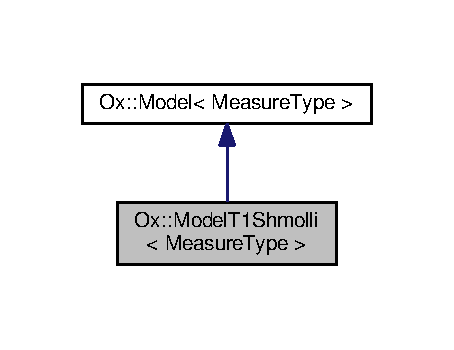
\includegraphics[width=219pt]{class_ox_1_1_model_t1_shmolli__inherit__graph}
\end{center}
\end{figure}


Collaboration diagram for Ox\+:\+:Model\+T1\+Shmolli$<$ Measure\+Type $>$\+:
\nopagebreak
\begin{figure}[H]
\begin{center}
\leavevmode
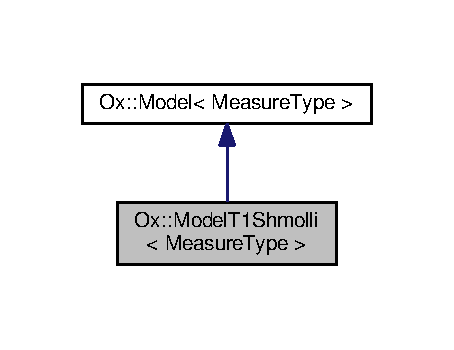
\includegraphics[width=219pt]{class_ox_1_1_model_t1_shmolli__coll__graph}
\end{center}
\end{figure}
\subsection*{Public Member Functions}
\begin{DoxyCompactItemize}
\item 
virtual Measure\+Type \hyperlink{class_ox_1_1_model_t1_shmolli_a72576d4db2ff938037c3d9d4fe25b9d7}{calc\+Model\+Value} (const Measure\+Type $\ast$parameters, Measure\+Type time)
\item 
virtual void \hyperlink{class_ox_1_1_model_t1_shmolli_ae393758f44f51e2fddae4c3c919fe4db}{calc\+L\+S\+Residuals} (const Measure\+Type $\ast$parameters, Measure\+Type $\ast$residuals)
\item 
virtual void \hyperlink{class_ox_1_1_model_t1_shmolli_a667e5c9088ba65e0cba506246671e3da}{calc\+L\+S\+Jacobian} (const Measure\+Type $\ast$parameters, Measure\+Type $\ast$jacobian)
\item 
virtual Measure\+Type \hyperlink{class_ox_1_1_model_t1_shmolli_a0f9b89832a6321b5b54abb9e219e803d}{calc\+Cost\+Value} (const Measure\+Type $\ast$parameters)
\item 
virtual void \hyperlink{class_ox_1_1_model_t1_shmolli_afaadbc879361f3ea674fe79a9fc1cf49}{calc\+Cost\+Derivative} (const Measure\+Type $\ast$parameters, Measure\+Type $\ast$derivative)
\item 
virtual \hyperlink{class_ox_1_1_model}{Model}$<$ Measure\+Type $>$ $\ast$ \hyperlink{class_ox_1_1_model_t1_shmolli_a846fb817183738d5c2b3f9f126c1597b}{new\+By\+Cloning} ()
\item 
virtual \hyperlink{class_ox_1_1_model_t1_shmolli_ad5dd9c59e049f1c356541ac278bc1e18}{$\sim$\+Model\+T1\+Shmolli} ()\hypertarget{class_ox_1_1_model_t1_shmolli_ad5dd9c59e049f1c356541ac278bc1e18}{}\label{class_ox_1_1_model_t1_shmolli_ad5dd9c59e049f1c356541ac278bc1e18}

\begin{DoxyCompactList}\small\item\em do not forget about the virtual destructor, see \href{https://stackoverflow.com/questions/461203/when-to-use-virtual-destructors}{\tt https\+://stackoverflow.\+com/questions/461203/when-\/to-\/use-\/virtual-\/destructors} \end{DoxyCompactList}\end{DoxyCompactItemize}
\subsection*{Public Attributes}
\begin{DoxyCompactItemize}
\item 
bool {\bfseries \+\_\+exp\+Abs\+Cost}\hypertarget{class_ox_1_1_model_t1_shmolli_a9ef12784ac237845296da239cd4517f2}{}\label{class_ox_1_1_model_t1_shmolli_a9ef12784ac237845296da239cd4517f2}

\item 
bool {\bfseries \+\_\+prevent\+Under\+Over\+Flow}\hypertarget{class_ox_1_1_model_t1_shmolli_aa7fd686c2f08a4ed27d33b934fcad37f}{}\label{class_ox_1_1_model_t1_shmolli_aa7fd686c2f08a4ed27d33b934fcad37f}

\item 
bool {\bfseries \+\_\+cost\+Heuristic}\hypertarget{class_ox_1_1_model_t1_shmolli_adc598e5bee08606512d2a823536f7b3d}{}\label{class_ox_1_1_model_t1_shmolli_adc598e5bee08606512d2a823536f7b3d}

\item 
bool {\bfseries \+\_\+root\+Median\+Square\+Cost}\hypertarget{class_ox_1_1_model_t1_shmolli_a043784373e50e27f8dfbdd42d82eb290}{}\label{class_ox_1_1_model_t1_shmolli_a043784373e50e27f8dfbdd42d82eb290}

\end{DoxyCompactItemize}
\subsection*{Additional Inherited Members}


\subsection{Detailed Description}
\subsubsection*{template$<$typename Measure\+Type$>$\\*
class Ox\+::\+Model\+T1\+Shmolli$<$ Measure\+Type $>$}

Container for a Calculator\+Shmolli model function $ A-B\exp(t/T_1^*) $, cost function and Least-\/\+Squares function and derivatives. 


\begin{DoxyTemplParams}{Template Parameters}
{\em Measure\+Type} & \\
\hline
\end{DoxyTemplParams}


\subsection{Member Function Documentation}
\index{Ox\+::\+Model\+T1\+Shmolli@{Ox\+::\+Model\+T1\+Shmolli}!calc\+Cost\+Derivative@{calc\+Cost\+Derivative}}
\index{calc\+Cost\+Derivative@{calc\+Cost\+Derivative}!Ox\+::\+Model\+T1\+Shmolli@{Ox\+::\+Model\+T1\+Shmolli}}
\subsubsection[{\texorpdfstring{calc\+Cost\+Derivative(const Measure\+Type $\ast$parameters, Measure\+Type $\ast$derivative)}{calcCostDerivative(const MeasureType *parameters, MeasureType *derivative)}}]{\setlength{\rightskip}{0pt plus 5cm}template$<$typename Measure\+Type $>$ void {\bf Ox\+::\+Model\+T1\+Shmolli}$<$ Measure\+Type $>$\+::calc\+Cost\+Derivative (
\begin{DoxyParamCaption}
\item[{const Measure\+Type $\ast$}]{parameters, }
\item[{Measure\+Type $\ast$}]{derivative}
\end{DoxyParamCaption}
)\hspace{0.3cm}{\ttfamily [virtual]}}\hypertarget{class_ox_1_1_model_t1_shmolli_afaadbc879361f3ea674fe79a9fc1cf49}{}\label{class_ox_1_1_model_t1_shmolli_afaadbc879361f3ea674fe79a9fc1cf49}
calc\+Cost\+Derivative the most important function of this class 
\begin{DoxyParams}{Parameters}
{\em derivative} & \\
\hline
\end{DoxyParams}


Implements \hyperlink{class_ox_1_1_model_a274f0efdbbc364e82bba7470f933eecd}{Ox\+::\+Model$<$ Measure\+Type $>$}.

\index{Ox\+::\+Model\+T1\+Shmolli@{Ox\+::\+Model\+T1\+Shmolli}!calc\+Cost\+Value@{calc\+Cost\+Value}}
\index{calc\+Cost\+Value@{calc\+Cost\+Value}!Ox\+::\+Model\+T1\+Shmolli@{Ox\+::\+Model\+T1\+Shmolli}}
\subsubsection[{\texorpdfstring{calc\+Cost\+Value(const Measure\+Type $\ast$parameters)}{calcCostValue(const MeasureType *parameters)}}]{\setlength{\rightskip}{0pt plus 5cm}template$<$typename Measure\+Type $>$ Measure\+Type {\bf Ox\+::\+Model\+T1\+Shmolli}$<$ Measure\+Type $>$\+::calc\+Cost\+Value (
\begin{DoxyParamCaption}
\item[{const Measure\+Type $\ast$}]{parameters}
\end{DoxyParamCaption}
)\hspace{0.3cm}{\ttfamily [virtual]}}\hypertarget{class_ox_1_1_model_t1_shmolli_a0f9b89832a6321b5b54abb9e219e803d}{}\label{class_ox_1_1_model_t1_shmolli_a0f9b89832a6321b5b54abb9e219e803d}
calc\+Cost\+Value the most important function of this class \begin{DoxyReturn}{Returns}

\end{DoxyReturn}


Implements \hyperlink{class_ox_1_1_model_aa5997cea7114d0e323e79956adb13ba4}{Ox\+::\+Model$<$ Measure\+Type $>$}.

\index{Ox\+::\+Model\+T1\+Shmolli@{Ox\+::\+Model\+T1\+Shmolli}!calc\+L\+S\+Jacobian@{calc\+L\+S\+Jacobian}}
\index{calc\+L\+S\+Jacobian@{calc\+L\+S\+Jacobian}!Ox\+::\+Model\+T1\+Shmolli@{Ox\+::\+Model\+T1\+Shmolli}}
\subsubsection[{\texorpdfstring{calc\+L\+S\+Jacobian(const Measure\+Type $\ast$parameters, Measure\+Type $\ast$jacobian)}{calcLSJacobian(const MeasureType *parameters, MeasureType *jacobian)}}]{\setlength{\rightskip}{0pt plus 5cm}template$<$typename Measure\+Type $>$ void {\bf Ox\+::\+Model\+T1\+Shmolli}$<$ Measure\+Type $>$\+::calc\+L\+S\+Jacobian (
\begin{DoxyParamCaption}
\item[{const Measure\+Type $\ast$}]{parameters, }
\item[{Measure\+Type $\ast$}]{jacobian}
\end{DoxyParamCaption}
)\hspace{0.3cm}{\ttfamily [virtual]}}\hypertarget{class_ox_1_1_model_t1_shmolli_a667e5c9088ba65e0cba506246671e3da}{}\label{class_ox_1_1_model_t1_shmolli_a667e5c9088ba65e0cba506246671e3da}
calc\+L\+S\+Jacobian the most important function of this class 
\begin{DoxyParams}{Parameters}
{\em jacobian} & -\/ 2d matrix stored as 1d array \\
\hline
\end{DoxyParams}


Implements \hyperlink{class_ox_1_1_model_a4cadb65b8416b4b30e91bf6db00737f3}{Ox\+::\+Model$<$ Measure\+Type $>$}.

\index{Ox\+::\+Model\+T1\+Shmolli@{Ox\+::\+Model\+T1\+Shmolli}!calc\+L\+S\+Residuals@{calc\+L\+S\+Residuals}}
\index{calc\+L\+S\+Residuals@{calc\+L\+S\+Residuals}!Ox\+::\+Model\+T1\+Shmolli@{Ox\+::\+Model\+T1\+Shmolli}}
\subsubsection[{\texorpdfstring{calc\+L\+S\+Residuals(const Measure\+Type $\ast$parameters, Measure\+Type $\ast$residuals)}{calcLSResiduals(const MeasureType *parameters, MeasureType *residuals)}}]{\setlength{\rightskip}{0pt plus 5cm}template$<$typename Measure\+Type $>$ void {\bf Ox\+::\+Model\+T1\+Shmolli}$<$ Measure\+Type $>$\+::calc\+L\+S\+Residuals (
\begin{DoxyParamCaption}
\item[{const Measure\+Type $\ast$}]{parameters, }
\item[{Measure\+Type $\ast$}]{residuals}
\end{DoxyParamCaption}
)\hspace{0.3cm}{\ttfamily [virtual]}}\hypertarget{class_ox_1_1_model_t1_shmolli_ae393758f44f51e2fddae4c3c919fe4db}{}\label{class_ox_1_1_model_t1_shmolli_ae393758f44f51e2fddae4c3c919fe4db}
calc\+L\+S\+Residuals the most important function of this class 
\begin{DoxyParams}{Parameters}
{\em residuals} & \\
\hline
\end{DoxyParams}


Implements \hyperlink{class_ox_1_1_model_a17e0ef71135350d4f61bef2a097fb586}{Ox\+::\+Model$<$ Measure\+Type $>$}.

\index{Ox\+::\+Model\+T1\+Shmolli@{Ox\+::\+Model\+T1\+Shmolli}!calc\+Model\+Value@{calc\+Model\+Value}}
\index{calc\+Model\+Value@{calc\+Model\+Value}!Ox\+::\+Model\+T1\+Shmolli@{Ox\+::\+Model\+T1\+Shmolli}}
\subsubsection[{\texorpdfstring{calc\+Model\+Value(const Measure\+Type $\ast$parameters, Measure\+Type time)}{calcModelValue(const MeasureType *parameters, MeasureType time)}}]{\setlength{\rightskip}{0pt plus 5cm}template$<$typename Measure\+Type $>$ Measure\+Type {\bf Ox\+::\+Model\+T1\+Shmolli}$<$ Measure\+Type $>$\+::calc\+Model\+Value (
\begin{DoxyParamCaption}
\item[{const Measure\+Type $\ast$}]{parameters, }
\item[{Measure\+Type}]{time}
\end{DoxyParamCaption}
)\hspace{0.3cm}{\ttfamily [virtual]}}\hypertarget{class_ox_1_1_model_t1_shmolli_a72576d4db2ff938037c3d9d4fe25b9d7}{}\label{class_ox_1_1_model_t1_shmolli_a72576d4db2ff938037c3d9d4fe25b9d7}
calc\+Model\+Value the most important function of this class 
\begin{DoxyParams}{Parameters}
{\em time} & \\
\hline
\end{DoxyParams}
\begin{DoxyReturn}{Returns}
model(time) 
\end{DoxyReturn}


Implements \hyperlink{class_ox_1_1_model_ae3a3f5bfeefd8a8c0c012e1761eac1f5}{Ox\+::\+Model$<$ Measure\+Type $>$}.

\index{Ox\+::\+Model\+T1\+Shmolli@{Ox\+::\+Model\+T1\+Shmolli}!new\+By\+Cloning@{new\+By\+Cloning}}
\index{new\+By\+Cloning@{new\+By\+Cloning}!Ox\+::\+Model\+T1\+Shmolli@{Ox\+::\+Model\+T1\+Shmolli}}
\subsubsection[{\texorpdfstring{new\+By\+Cloning()}{newByCloning()}}]{\setlength{\rightskip}{0pt plus 5cm}template$<$typename Measure\+Type$>$ virtual {\bf Model}$<$Measure\+Type$>$$\ast$ {\bf Ox\+::\+Model\+T1\+Shmolli}$<$ Measure\+Type $>$\+::new\+By\+Cloning (
\begin{DoxyParamCaption}
{}
\end{DoxyParamCaption}
)\hspace{0.3cm}{\ttfamily [inline]}, {\ttfamily [virtual]}}\hypertarget{class_ox_1_1_model_t1_shmolli_a846fb817183738d5c2b3f9f126c1597b}{}\label{class_ox_1_1_model_t1_shmolli_a846fb817183738d5c2b3f9f126c1597b}
cloning \begin{DoxyReturn}{Returns}

\end{DoxyReturn}


Implements \hyperlink{class_ox_1_1_model_a694868476dd17a4d203f4ebc57047d2f}{Ox\+::\+Model$<$ Measure\+Type $>$}.



The documentation for this class was generated from the following files\+:\begin{DoxyCompactItemize}
\item 
lib/\hyperlink{_ox_model_t1_shmolli_8h}{Ox\+Model\+T1\+Shmolli.\+h}\item 
lib/\hyperlink{_ox_model_t1_shmolli_8hxx}{Ox\+Model\+T1\+Shmolli.\+hxx}\end{DoxyCompactItemize}

\hypertarget{class_ox_1_1_model_t1_three_param}{\section{Ox\-:\-:Model\-T1\-Three\-Param$<$ Measure\-Type $>$ Class Template Reference}
\label{class_ox_1_1_model_t1_three_param}\index{Ox\-::\-Model\-T1\-Three\-Param$<$ Measure\-Type $>$@{Ox\-::\-Model\-T1\-Three\-Param$<$ Measure\-Type $>$}}
}


Container for a Three\-Param model function $ A-B\exp(t/T_1^*) $, cost function and Least-\/\-Squares function and derivatives.  




{\ttfamily \#include $<$Ox\-Model\-T1\-Three\-Param.\-h$>$}



Inheritance diagram for Ox\-:\-:Model\-T1\-Three\-Param$<$ Measure\-Type $>$\-:
\nopagebreak
\begin{figure}[H]
\begin{center}
\leavevmode
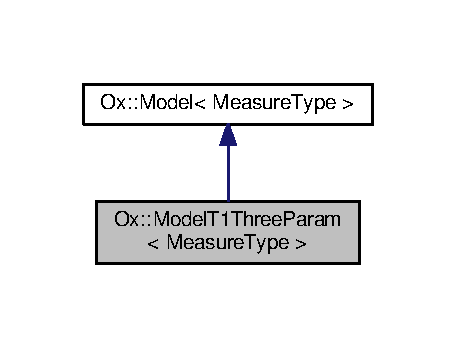
\includegraphics[width=218pt]{class_ox_1_1_model_t1_three_param__inherit__graph}
\end{center}
\end{figure}


Collaboration diagram for Ox\-:\-:Model\-T1\-Three\-Param$<$ Measure\-Type $>$\-:
\nopagebreak
\begin{figure}[H]
\begin{center}
\leavevmode
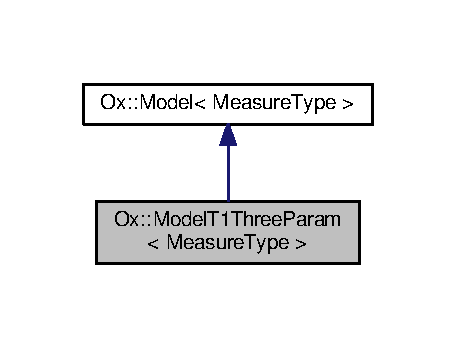
\includegraphics[width=218pt]{class_ox_1_1_model_t1_three_param__coll__graph}
\end{center}
\end{figure}
\subsection*{Public Member Functions}
\begin{DoxyCompactItemize}
\item 
virtual Measure\-Type \hyperlink{class_ox_1_1_model_t1_three_param_a4b2e40499a77399cc3dd74fbe9a02aee}{calc\-Model\-Value} (const Measure\-Type $\ast$parameters, Measure\-Type time)
\item 
virtual void \hyperlink{class_ox_1_1_model_t1_three_param_abef151c12e9b7d49e23955dd1ae9c992}{calc\-L\-S\-Residuals} (const Measure\-Type $\ast$parameters, Measure\-Type $\ast$residuals)
\item 
virtual void \hyperlink{class_ox_1_1_model_t1_three_param_a2b6268cb77c6a9d95c7861641cd3a2d5}{calc\-L\-S\-Jacobian} (const Measure\-Type $\ast$parameters, Measure\-Type $\ast$jacobian)
\item 
virtual Measure\-Type \hyperlink{class_ox_1_1_model_t1_three_param_ad417e4455caae28f1364f82b5f8f37d5}{calc\-Cost\-Value} (const Measure\-Type $\ast$parameters)
\item 
virtual void \hyperlink{class_ox_1_1_model_t1_three_param_a7bd09162c315aa491af661cf8d88bcdd}{calc\-Cost\-Derivative} (const Measure\-Type $\ast$parameters, Measure\-Type $\ast$derivative)
\item 
virtual \hyperlink{class_ox_1_1_model}{Model}$<$ Measure\-Type $>$ $\ast$ \hyperlink{class_ox_1_1_model_t1_three_param_afc6ffe41934c513e12a45cc5821fddca}{new\-By\-Cloning} ()
\item 
\hypertarget{class_ox_1_1_model_t1_three_param_a533739a9eda1cb9d006e292bae466082}{virtual \hyperlink{class_ox_1_1_model_t1_three_param_a533739a9eda1cb9d006e292bae466082}{$\sim$\-Model\-T1\-Three\-Param} ()}\label{class_ox_1_1_model_t1_three_param_a533739a9eda1cb9d006e292bae466082}

\begin{DoxyCompactList}\small\item\em do not forget about the virtual destructor, see \href{https://stackoverflow.com/questions/461203/when-to-use-virtual-destructors}{\tt https\-://stackoverflow.\-com/questions/461203/when-\/to-\/use-\/virtual-\/destructors} \end{DoxyCompactList}\end{DoxyCompactItemize}
\subsection*{Additional Inherited Members}


\subsection{Detailed Description}
\subsubsection*{template$<$typename Measure\-Type$>$class Ox\-::\-Model\-T1\-Three\-Param$<$ Measure\-Type $>$}

Container for a Three\-Param model function $ A-B\exp(t/T_1^*) $, cost function and Least-\/\-Squares function and derivatives. 


\begin{DoxyTemplParams}{Template Parameters}
{\em Measure\-Type} & \\
\hline
\end{DoxyTemplParams}


\subsection{Member Function Documentation}
\hypertarget{class_ox_1_1_model_t1_three_param_a7bd09162c315aa491af661cf8d88bcdd}{\index{Ox\-::\-Model\-T1\-Three\-Param@{Ox\-::\-Model\-T1\-Three\-Param}!calc\-Cost\-Derivative@{calc\-Cost\-Derivative}}
\index{calc\-Cost\-Derivative@{calc\-Cost\-Derivative}!Ox::ModelT1ThreeParam@{Ox\-::\-Model\-T1\-Three\-Param}}
\subsubsection[{calc\-Cost\-Derivative}]{\setlength{\rightskip}{0pt plus 5cm}template$<$typename Measure\-Type $>$ void {\bf Ox\-::\-Model\-T1\-Three\-Param}$<$ Measure\-Type $>$\-::calc\-Cost\-Derivative (
\begin{DoxyParamCaption}
\item[{const Measure\-Type $\ast$}]{parameters, }
\item[{Measure\-Type $\ast$}]{derivative}
\end{DoxyParamCaption}
)\hspace{0.3cm}{\ttfamily [virtual]}}}\label{class_ox_1_1_model_t1_three_param_a7bd09162c315aa491af661cf8d88bcdd}
calc\-Cost\-Derivative the most important function of this class 
\begin{DoxyParams}{Parameters}
{\em derivative} & \\
\hline
\end{DoxyParams}


Implements \hyperlink{class_ox_1_1_model_a274f0efdbbc364e82bba7470f933eecd}{Ox\-::\-Model$<$ Measure\-Type $>$}.

\hypertarget{class_ox_1_1_model_t1_three_param_ad417e4455caae28f1364f82b5f8f37d5}{\index{Ox\-::\-Model\-T1\-Three\-Param@{Ox\-::\-Model\-T1\-Three\-Param}!calc\-Cost\-Value@{calc\-Cost\-Value}}
\index{calc\-Cost\-Value@{calc\-Cost\-Value}!Ox::ModelT1ThreeParam@{Ox\-::\-Model\-T1\-Three\-Param}}
\subsubsection[{calc\-Cost\-Value}]{\setlength{\rightskip}{0pt plus 5cm}template$<$typename Measure\-Type $>$ Measure\-Type {\bf Ox\-::\-Model\-T1\-Three\-Param}$<$ Measure\-Type $>$\-::calc\-Cost\-Value (
\begin{DoxyParamCaption}
\item[{const Measure\-Type $\ast$}]{parameters}
\end{DoxyParamCaption}
)\hspace{0.3cm}{\ttfamily [virtual]}}}\label{class_ox_1_1_model_t1_three_param_ad417e4455caae28f1364f82b5f8f37d5}
calc\-Cost\-Value the most important function of this class \begin{DoxyReturn}{Returns}

\end{DoxyReturn}


Implements \hyperlink{class_ox_1_1_model_aa5997cea7114d0e323e79956adb13ba4}{Ox\-::\-Model$<$ Measure\-Type $>$}.

\hypertarget{class_ox_1_1_model_t1_three_param_a2b6268cb77c6a9d95c7861641cd3a2d5}{\index{Ox\-::\-Model\-T1\-Three\-Param@{Ox\-::\-Model\-T1\-Three\-Param}!calc\-L\-S\-Jacobian@{calc\-L\-S\-Jacobian}}
\index{calc\-L\-S\-Jacobian@{calc\-L\-S\-Jacobian}!Ox::ModelT1ThreeParam@{Ox\-::\-Model\-T1\-Three\-Param}}
\subsubsection[{calc\-L\-S\-Jacobian}]{\setlength{\rightskip}{0pt plus 5cm}template$<$typename Measure\-Type $>$ void {\bf Ox\-::\-Model\-T1\-Three\-Param}$<$ Measure\-Type $>$\-::calc\-L\-S\-Jacobian (
\begin{DoxyParamCaption}
\item[{const Measure\-Type $\ast$}]{parameters, }
\item[{Measure\-Type $\ast$}]{jacobian}
\end{DoxyParamCaption}
)\hspace{0.3cm}{\ttfamily [virtual]}}}\label{class_ox_1_1_model_t1_three_param_a2b6268cb77c6a9d95c7861641cd3a2d5}
calc\-L\-S\-Jacobian the most important function of this class 
\begin{DoxyParams}{Parameters}
{\em jacobian} & -\/ 2d matrix stored as 1d array \\
\hline
\end{DoxyParams}


Implements \hyperlink{class_ox_1_1_model_a4cadb65b8416b4b30e91bf6db00737f3}{Ox\-::\-Model$<$ Measure\-Type $>$}.

\hypertarget{class_ox_1_1_model_t1_three_param_abef151c12e9b7d49e23955dd1ae9c992}{\index{Ox\-::\-Model\-T1\-Three\-Param@{Ox\-::\-Model\-T1\-Three\-Param}!calc\-L\-S\-Residuals@{calc\-L\-S\-Residuals}}
\index{calc\-L\-S\-Residuals@{calc\-L\-S\-Residuals}!Ox::ModelT1ThreeParam@{Ox\-::\-Model\-T1\-Three\-Param}}
\subsubsection[{calc\-L\-S\-Residuals}]{\setlength{\rightskip}{0pt plus 5cm}template$<$typename Measure\-Type $>$ void {\bf Ox\-::\-Model\-T1\-Three\-Param}$<$ Measure\-Type $>$\-::calc\-L\-S\-Residuals (
\begin{DoxyParamCaption}
\item[{const Measure\-Type $\ast$}]{parameters, }
\item[{Measure\-Type $\ast$}]{residuals}
\end{DoxyParamCaption}
)\hspace{0.3cm}{\ttfamily [virtual]}}}\label{class_ox_1_1_model_t1_three_param_abef151c12e9b7d49e23955dd1ae9c992}
calc\-L\-S\-Residuals the most important function of this class 
\begin{DoxyParams}{Parameters}
{\em residuals} & \\
\hline
\end{DoxyParams}


Implements \hyperlink{class_ox_1_1_model_a17e0ef71135350d4f61bef2a097fb586}{Ox\-::\-Model$<$ Measure\-Type $>$}.

\hypertarget{class_ox_1_1_model_t1_three_param_a4b2e40499a77399cc3dd74fbe9a02aee}{\index{Ox\-::\-Model\-T1\-Three\-Param@{Ox\-::\-Model\-T1\-Three\-Param}!calc\-Model\-Value@{calc\-Model\-Value}}
\index{calc\-Model\-Value@{calc\-Model\-Value}!Ox::ModelT1ThreeParam@{Ox\-::\-Model\-T1\-Three\-Param}}
\subsubsection[{calc\-Model\-Value}]{\setlength{\rightskip}{0pt plus 5cm}template$<$typename Measure\-Type $>$ Measure\-Type {\bf Ox\-::\-Model\-T1\-Three\-Param}$<$ Measure\-Type $>$\-::calc\-Model\-Value (
\begin{DoxyParamCaption}
\item[{const Measure\-Type $\ast$}]{parameters, }
\item[{Measure\-Type}]{time}
\end{DoxyParamCaption}
)\hspace{0.3cm}{\ttfamily [virtual]}}}\label{class_ox_1_1_model_t1_three_param_a4b2e40499a77399cc3dd74fbe9a02aee}
calc\-Model\-Value the most important function of this class 
\begin{DoxyParams}{Parameters}
{\em time} & \\
\hline
\end{DoxyParams}
\begin{DoxyReturn}{Returns}
model(time) 
\end{DoxyReturn}


Implements \hyperlink{class_ox_1_1_model_ae3a3f5bfeefd8a8c0c012e1761eac1f5}{Ox\-::\-Model$<$ Measure\-Type $>$}.

\hypertarget{class_ox_1_1_model_t1_three_param_afc6ffe41934c513e12a45cc5821fddca}{\index{Ox\-::\-Model\-T1\-Three\-Param@{Ox\-::\-Model\-T1\-Three\-Param}!new\-By\-Cloning@{new\-By\-Cloning}}
\index{new\-By\-Cloning@{new\-By\-Cloning}!Ox::ModelT1ThreeParam@{Ox\-::\-Model\-T1\-Three\-Param}}
\subsubsection[{new\-By\-Cloning}]{\setlength{\rightskip}{0pt plus 5cm}template$<$typename Measure\-Type$>$ virtual {\bf Model}$<$Measure\-Type$>$$\ast$ {\bf Ox\-::\-Model\-T1\-Three\-Param}$<$ Measure\-Type $>$\-::new\-By\-Cloning (
\begin{DoxyParamCaption}
{}
\end{DoxyParamCaption}
)\hspace{0.3cm}{\ttfamily [inline]}, {\ttfamily [virtual]}}}\label{class_ox_1_1_model_t1_three_param_afc6ffe41934c513e12a45cc5821fddca}
cloning \begin{DoxyReturn}{Returns}

\end{DoxyReturn}


Implements \hyperlink{class_ox_1_1_model_a694868476dd17a4d203f4ebc57047d2f}{Ox\-::\-Model$<$ Measure\-Type $>$}.



The documentation for this class was generated from the following files\-:\begin{DoxyCompactItemize}
\item 
lib/\hyperlink{_ox_model_t1_three_param_8h}{Ox\-Model\-T1\-Three\-Param.\-h}\item 
lib/\hyperlink{_ox_model_t1_three_param_8hxx}{Ox\-Model\-T1\-Three\-Param.\-hxx}\end{DoxyCompactItemize}

\hypertarget{class_ox_1_1_model_t1_two_param}{\section{Ox\-:\-:Model\-T1\-Two\-Param$<$ Measure\-Type $>$ Class Template Reference}
\label{class_ox_1_1_model_t1_two_param}\index{Ox\-::\-Model\-T1\-Two\-Param$<$ Measure\-Type $>$@{Ox\-::\-Model\-T1\-Two\-Param$<$ Measure\-Type $>$}}
}


Container for a Two\-Param model function $ A(1 - exp( -time / T1 )) $, cost function and Least-\/\-Squares function and derivatives.  




{\ttfamily \#include $<$Ox\-Model\-T1\-Two\-Param.\-h$>$}



Inheritance diagram for Ox\-:\-:Model\-T1\-Two\-Param$<$ Measure\-Type $>$\-:
\nopagebreak
\begin{figure}[H]
\begin{center}
\leavevmode
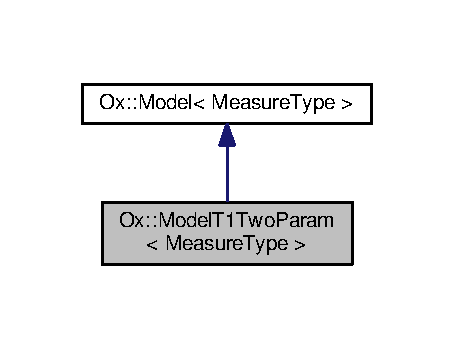
\includegraphics[width=218pt]{class_ox_1_1_model_t1_two_param__inherit__graph}
\end{center}
\end{figure}


Collaboration diagram for Ox\-:\-:Model\-T1\-Two\-Param$<$ Measure\-Type $>$\-:
\nopagebreak
\begin{figure}[H]
\begin{center}
\leavevmode
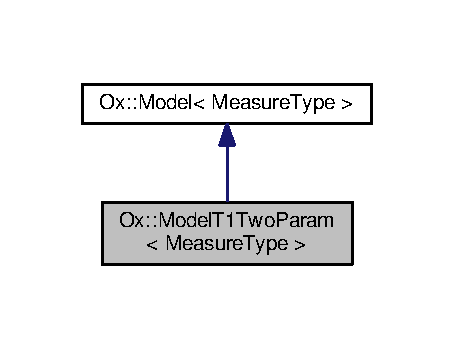
\includegraphics[width=218pt]{class_ox_1_1_model_t1_two_param__coll__graph}
\end{center}
\end{figure}
\subsection*{Public Member Functions}
\begin{DoxyCompactItemize}
\item 
virtual Measure\-Type \hyperlink{class_ox_1_1_model_t1_two_param_aaa8218e3d53e1913589d272bcbb62b47}{calc\-Model\-Value} (const Measure\-Type $\ast$parameters, Measure\-Type time)
\item 
virtual void \hyperlink{class_ox_1_1_model_t1_two_param_a8c02d34fac5a35310f6ee60209f70d45}{calc\-L\-S\-Residuals} (const Measure\-Type $\ast$parameters, Measure\-Type $\ast$residuals)
\item 
virtual void \hyperlink{class_ox_1_1_model_t1_two_param_af5952a47062e6edffe78f8594cc220e4}{calc\-L\-S\-Jacobian} (const Measure\-Type $\ast$parameters, Measure\-Type $\ast$jacobian)
\item 
virtual Measure\-Type \hyperlink{class_ox_1_1_model_t1_two_param_ab4ec672167094e84f2fddc5d052d528c}{calc\-Cost\-Value} (const Measure\-Type $\ast$parameters)
\item 
virtual void \hyperlink{class_ox_1_1_model_t1_two_param_a328e0fdc6b5769ecc3327596c9b12be3}{calc\-Cost\-Derivative} (const Measure\-Type $\ast$parameters, Measure\-Type $\ast$derivative)
\item 
virtual \hyperlink{class_ox_1_1_model}{Model}$<$ Measure\-Type $>$ $\ast$ \hyperlink{class_ox_1_1_model_t1_two_param_aa090c6834141f00a966eebd6b0415e44}{new\-By\-Cloning} ()
\item 
\hypertarget{class_ox_1_1_model_t1_two_param_ae6870d10db397016649989969c613f32}{virtual \hyperlink{class_ox_1_1_model_t1_two_param_ae6870d10db397016649989969c613f32}{$\sim$\-Model\-T1\-Two\-Param} ()}\label{class_ox_1_1_model_t1_two_param_ae6870d10db397016649989969c613f32}

\begin{DoxyCompactList}\small\item\em do not forget about the virtual destructor, see \href{https://stackoverflow.com/questions/461203/when-to-use-virtual-destructors}{\tt https\-://stackoverflow.\-com/questions/461203/when-\/to-\/use-\/virtual-\/destructors} \end{DoxyCompactList}\end{DoxyCompactItemize}
\subsection*{Additional Inherited Members}


\subsection{Detailed Description}
\subsubsection*{template$<$typename Measure\-Type$>$class Ox\-::\-Model\-T1\-Two\-Param$<$ Measure\-Type $>$}

Container for a Two\-Param model function $ A(1 - exp( -time / T1 )) $, cost function and Least-\/\-Squares function and derivatives. 


\begin{DoxyTemplParams}{Template Parameters}
{\em Measure\-Type} & \\
\hline
\end{DoxyTemplParams}


\subsection{Member Function Documentation}
\hypertarget{class_ox_1_1_model_t1_two_param_a328e0fdc6b5769ecc3327596c9b12be3}{\index{Ox\-::\-Model\-T1\-Two\-Param@{Ox\-::\-Model\-T1\-Two\-Param}!calc\-Cost\-Derivative@{calc\-Cost\-Derivative}}
\index{calc\-Cost\-Derivative@{calc\-Cost\-Derivative}!Ox::ModelT1TwoParam@{Ox\-::\-Model\-T1\-Two\-Param}}
\subsubsection[{calc\-Cost\-Derivative}]{\setlength{\rightskip}{0pt plus 5cm}template$<$typename Measure\-Type $>$ void {\bf Ox\-::\-Model\-T1\-Two\-Param}$<$ Measure\-Type $>$\-::calc\-Cost\-Derivative (
\begin{DoxyParamCaption}
\item[{const Measure\-Type $\ast$}]{parameters, }
\item[{Measure\-Type $\ast$}]{derivative}
\end{DoxyParamCaption}
)\hspace{0.3cm}{\ttfamily [virtual]}}}\label{class_ox_1_1_model_t1_two_param_a328e0fdc6b5769ecc3327596c9b12be3}
calc\-Cost\-Derivative the most important function of this class 
\begin{DoxyParams}{Parameters}
{\em derivative} & \\
\hline
\end{DoxyParams}


Implements \hyperlink{class_ox_1_1_model_a274f0efdbbc364e82bba7470f933eecd}{Ox\-::\-Model$<$ Measure\-Type $>$}.

\hypertarget{class_ox_1_1_model_t1_two_param_ab4ec672167094e84f2fddc5d052d528c}{\index{Ox\-::\-Model\-T1\-Two\-Param@{Ox\-::\-Model\-T1\-Two\-Param}!calc\-Cost\-Value@{calc\-Cost\-Value}}
\index{calc\-Cost\-Value@{calc\-Cost\-Value}!Ox::ModelT1TwoParam@{Ox\-::\-Model\-T1\-Two\-Param}}
\subsubsection[{calc\-Cost\-Value}]{\setlength{\rightskip}{0pt plus 5cm}template$<$typename Measure\-Type $>$ Measure\-Type {\bf Ox\-::\-Model\-T1\-Two\-Param}$<$ Measure\-Type $>$\-::calc\-Cost\-Value (
\begin{DoxyParamCaption}
\item[{const Measure\-Type $\ast$}]{parameters}
\end{DoxyParamCaption}
)\hspace{0.3cm}{\ttfamily [virtual]}}}\label{class_ox_1_1_model_t1_two_param_ab4ec672167094e84f2fddc5d052d528c}
calc\-Cost\-Value the most important function of this class \begin{DoxyReturn}{Returns}

\end{DoxyReturn}


Implements \hyperlink{class_ox_1_1_model_aa5997cea7114d0e323e79956adb13ba4}{Ox\-::\-Model$<$ Measure\-Type $>$}.

\hypertarget{class_ox_1_1_model_t1_two_param_af5952a47062e6edffe78f8594cc220e4}{\index{Ox\-::\-Model\-T1\-Two\-Param@{Ox\-::\-Model\-T1\-Two\-Param}!calc\-L\-S\-Jacobian@{calc\-L\-S\-Jacobian}}
\index{calc\-L\-S\-Jacobian@{calc\-L\-S\-Jacobian}!Ox::ModelT1TwoParam@{Ox\-::\-Model\-T1\-Two\-Param}}
\subsubsection[{calc\-L\-S\-Jacobian}]{\setlength{\rightskip}{0pt plus 5cm}template$<$typename Measure\-Type $>$ void {\bf Ox\-::\-Model\-T1\-Two\-Param}$<$ Measure\-Type $>$\-::calc\-L\-S\-Jacobian (
\begin{DoxyParamCaption}
\item[{const Measure\-Type $\ast$}]{parameters, }
\item[{Measure\-Type $\ast$}]{jacobian}
\end{DoxyParamCaption}
)\hspace{0.3cm}{\ttfamily [virtual]}}}\label{class_ox_1_1_model_t1_two_param_af5952a47062e6edffe78f8594cc220e4}
calc\-L\-S\-Jacobian the most important function of this class 
\begin{DoxyParams}{Parameters}
{\em jacobian} & -\/ 2d matrix stored as 1d array \\
\hline
\end{DoxyParams}


Implements \hyperlink{class_ox_1_1_model_a4cadb65b8416b4b30e91bf6db00737f3}{Ox\-::\-Model$<$ Measure\-Type $>$}.

\hypertarget{class_ox_1_1_model_t1_two_param_a8c02d34fac5a35310f6ee60209f70d45}{\index{Ox\-::\-Model\-T1\-Two\-Param@{Ox\-::\-Model\-T1\-Two\-Param}!calc\-L\-S\-Residuals@{calc\-L\-S\-Residuals}}
\index{calc\-L\-S\-Residuals@{calc\-L\-S\-Residuals}!Ox::ModelT1TwoParam@{Ox\-::\-Model\-T1\-Two\-Param}}
\subsubsection[{calc\-L\-S\-Residuals}]{\setlength{\rightskip}{0pt plus 5cm}template$<$typename Measure\-Type $>$ void {\bf Ox\-::\-Model\-T1\-Two\-Param}$<$ Measure\-Type $>$\-::calc\-L\-S\-Residuals (
\begin{DoxyParamCaption}
\item[{const Measure\-Type $\ast$}]{parameters, }
\item[{Measure\-Type $\ast$}]{residuals}
\end{DoxyParamCaption}
)\hspace{0.3cm}{\ttfamily [virtual]}}}\label{class_ox_1_1_model_t1_two_param_a8c02d34fac5a35310f6ee60209f70d45}
calc\-L\-S\-Residuals the most important function of this class 
\begin{DoxyParams}{Parameters}
{\em residuals} & \\
\hline
\end{DoxyParams}


Implements \hyperlink{class_ox_1_1_model_a17e0ef71135350d4f61bef2a097fb586}{Ox\-::\-Model$<$ Measure\-Type $>$}.

\hypertarget{class_ox_1_1_model_t1_two_param_aaa8218e3d53e1913589d272bcbb62b47}{\index{Ox\-::\-Model\-T1\-Two\-Param@{Ox\-::\-Model\-T1\-Two\-Param}!calc\-Model\-Value@{calc\-Model\-Value}}
\index{calc\-Model\-Value@{calc\-Model\-Value}!Ox::ModelT1TwoParam@{Ox\-::\-Model\-T1\-Two\-Param}}
\subsubsection[{calc\-Model\-Value}]{\setlength{\rightskip}{0pt plus 5cm}template$<$typename Measure\-Type $>$ Measure\-Type {\bf Ox\-::\-Model\-T1\-Two\-Param}$<$ Measure\-Type $>$\-::calc\-Model\-Value (
\begin{DoxyParamCaption}
\item[{const Measure\-Type $\ast$}]{parameters, }
\item[{Measure\-Type}]{time}
\end{DoxyParamCaption}
)\hspace{0.3cm}{\ttfamily [virtual]}}}\label{class_ox_1_1_model_t1_two_param_aaa8218e3d53e1913589d272bcbb62b47}
calc\-Model\-Value the most important function of this class 
\begin{DoxyParams}{Parameters}
{\em time} & \\
\hline
\end{DoxyParams}
\begin{DoxyReturn}{Returns}
model(time) 
\end{DoxyReturn}


Implements \hyperlink{class_ox_1_1_model_ae3a3f5bfeefd8a8c0c012e1761eac1f5}{Ox\-::\-Model$<$ Measure\-Type $>$}.

\hypertarget{class_ox_1_1_model_t1_two_param_aa090c6834141f00a966eebd6b0415e44}{\index{Ox\-::\-Model\-T1\-Two\-Param@{Ox\-::\-Model\-T1\-Two\-Param}!new\-By\-Cloning@{new\-By\-Cloning}}
\index{new\-By\-Cloning@{new\-By\-Cloning}!Ox::ModelT1TwoParam@{Ox\-::\-Model\-T1\-Two\-Param}}
\subsubsection[{new\-By\-Cloning}]{\setlength{\rightskip}{0pt plus 5cm}template$<$typename Measure\-Type$>$ virtual {\bf Model}$<$Measure\-Type$>$$\ast$ {\bf Ox\-::\-Model\-T1\-Two\-Param}$<$ Measure\-Type $>$\-::new\-By\-Cloning (
\begin{DoxyParamCaption}
{}
\end{DoxyParamCaption}
)\hspace{0.3cm}{\ttfamily [inline]}, {\ttfamily [virtual]}}}\label{class_ox_1_1_model_t1_two_param_aa090c6834141f00a966eebd6b0415e44}
cloning \begin{DoxyReturn}{Returns}

\end{DoxyReturn}


Implements \hyperlink{class_ox_1_1_model_a694868476dd17a4d203f4ebc57047d2f}{Ox\-::\-Model$<$ Measure\-Type $>$}.



The documentation for this class was generated from the following files\-:\begin{DoxyCompactItemize}
\item 
lib/\hyperlink{_ox_model_t1_two_param_8h}{Ox\-Model\-T1\-Two\-Param.\-h}\item 
lib/\hyperlink{_ox_model_t1_two_param_8hxx}{Ox\-Model\-T1\-Two\-Param.\-hxx}\end{DoxyCompactItemize}

\hypertarget{class_ox_1_1_model_t2_three_param}{\section{Ox\-:\-:Model\-T2\-Three\-Param$<$ Measure\-Type $>$ Class Template Reference}
\label{class_ox_1_1_model_t2_three_param}\index{Ox\-::\-Model\-T2\-Three\-Param$<$ Measure\-Type $>$@{Ox\-::\-Model\-T2\-Three\-Param$<$ Measure\-Type $>$}}
}


Container for a Three\-Param model function $ A + B\exp(t/T_2) $, cost function and Least-\/\-Squares function and derivatives.  




{\ttfamily \#include $<$Ox\-Model\-T2\-Three\-Param.\-h$>$}



Inheritance diagram for Ox\-:\-:Model\-T2\-Three\-Param$<$ Measure\-Type $>$\-:
\nopagebreak
\begin{figure}[H]
\begin{center}
\leavevmode
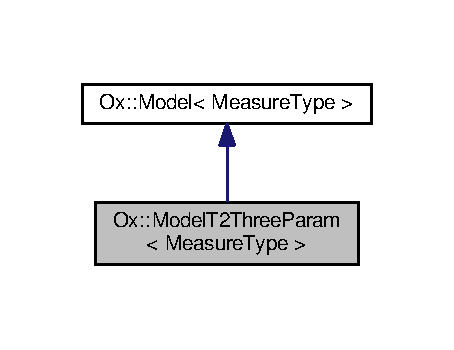
\includegraphics[width=218pt]{class_ox_1_1_model_t2_three_param__inherit__graph}
\end{center}
\end{figure}


Collaboration diagram for Ox\-:\-:Model\-T2\-Three\-Param$<$ Measure\-Type $>$\-:
\nopagebreak
\begin{figure}[H]
\begin{center}
\leavevmode
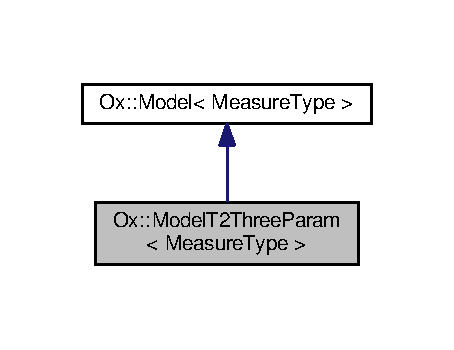
\includegraphics[width=218pt]{class_ox_1_1_model_t2_three_param__coll__graph}
\end{center}
\end{figure}
\subsection*{Public Member Functions}
\begin{DoxyCompactItemize}
\item 
virtual Measure\-Type \hyperlink{class_ox_1_1_model_t2_three_param_a2ed5138a6db7e8b64c5c8d8275de70ac}{calc\-Model\-Value} (const Measure\-Type $\ast$parameters, Measure\-Type time)
\item 
virtual void \hyperlink{class_ox_1_1_model_t2_three_param_af959d697820c70df520f987ba5e75b78}{calc\-L\-S\-Residuals} (const Measure\-Type $\ast$parameters, Measure\-Type $\ast$residuals)
\item 
virtual void \hyperlink{class_ox_1_1_model_t2_three_param_a727daa3a07d63fc3efbf0559ce32de9b}{calc\-L\-S\-Jacobian} (const Measure\-Type $\ast$parameters, Measure\-Type $\ast$jacobian)
\item 
virtual Measure\-Type \hyperlink{class_ox_1_1_model_t2_three_param_afa54ff1c8de4f2c2cf2fd50e3e357e2b}{calc\-Cost\-Value} (const Measure\-Type $\ast$parameters)
\item 
virtual void \hyperlink{class_ox_1_1_model_t2_three_param_a296bdf8378923d3e501c6e929608baca}{calc\-Cost\-Derivative} (const Measure\-Type $\ast$parameters, Measure\-Type $\ast$derivative)
\item 
virtual \hyperlink{class_ox_1_1_model}{Model}$<$ Measure\-Type $>$ $\ast$ \hyperlink{class_ox_1_1_model_t2_three_param_a7a6d2bae4e394a99e9e8943af9f344d0}{new\-By\-Cloning} ()
\item 
\hypertarget{class_ox_1_1_model_t2_three_param_a504f1b6e964c67bbf251469f2ae880ff}{virtual \hyperlink{class_ox_1_1_model_t2_three_param_a504f1b6e964c67bbf251469f2ae880ff}{$\sim$\-Model\-T2\-Three\-Param} ()}\label{class_ox_1_1_model_t2_three_param_a504f1b6e964c67bbf251469f2ae880ff}

\begin{DoxyCompactList}\small\item\em do not forget about the virtual destructor, see \href{https://stackoverflow.com/questions/461203/when-to-use-virtual-destructors}{\tt https\-://stackoverflow.\-com/questions/461203/when-\/to-\/use-\/virtual-\/destructors} \end{DoxyCompactList}\end{DoxyCompactItemize}
\subsection*{Additional Inherited Members}


\subsection{Detailed Description}
\subsubsection*{template$<$typename Measure\-Type$>$class Ox\-::\-Model\-T2\-Three\-Param$<$ Measure\-Type $>$}

Container for a Three\-Param model function $ A + B\exp(t/T_2) $, cost function and Least-\/\-Squares function and derivatives. 


\begin{DoxyTemplParams}{Template Parameters}
{\em Measure\-Type} & \\
\hline
\end{DoxyTemplParams}


\subsection{Member Function Documentation}
\hypertarget{class_ox_1_1_model_t2_three_param_a296bdf8378923d3e501c6e929608baca}{\index{Ox\-::\-Model\-T2\-Three\-Param@{Ox\-::\-Model\-T2\-Three\-Param}!calc\-Cost\-Derivative@{calc\-Cost\-Derivative}}
\index{calc\-Cost\-Derivative@{calc\-Cost\-Derivative}!Ox::ModelT2ThreeParam@{Ox\-::\-Model\-T2\-Three\-Param}}
\subsubsection[{calc\-Cost\-Derivative}]{\setlength{\rightskip}{0pt plus 5cm}template$<$typename Measure\-Type $>$ void {\bf Ox\-::\-Model\-T2\-Three\-Param}$<$ Measure\-Type $>$\-::calc\-Cost\-Derivative (
\begin{DoxyParamCaption}
\item[{const Measure\-Type $\ast$}]{parameters, }
\item[{Measure\-Type $\ast$}]{derivative}
\end{DoxyParamCaption}
)\hspace{0.3cm}{\ttfamily [virtual]}}}\label{class_ox_1_1_model_t2_three_param_a296bdf8378923d3e501c6e929608baca}
calc\-Cost\-Derivative the most important function of this class 
\begin{DoxyParams}{Parameters}
{\em derivative} & \\
\hline
\end{DoxyParams}


Implements \hyperlink{class_ox_1_1_model_a274f0efdbbc364e82bba7470f933eecd}{Ox\-::\-Model$<$ Measure\-Type $>$}.

\hypertarget{class_ox_1_1_model_t2_three_param_afa54ff1c8de4f2c2cf2fd50e3e357e2b}{\index{Ox\-::\-Model\-T2\-Three\-Param@{Ox\-::\-Model\-T2\-Three\-Param}!calc\-Cost\-Value@{calc\-Cost\-Value}}
\index{calc\-Cost\-Value@{calc\-Cost\-Value}!Ox::ModelT2ThreeParam@{Ox\-::\-Model\-T2\-Three\-Param}}
\subsubsection[{calc\-Cost\-Value}]{\setlength{\rightskip}{0pt plus 5cm}template$<$typename Measure\-Type $>$ Measure\-Type {\bf Ox\-::\-Model\-T2\-Three\-Param}$<$ Measure\-Type $>$\-::calc\-Cost\-Value (
\begin{DoxyParamCaption}
\item[{const Measure\-Type $\ast$}]{parameters}
\end{DoxyParamCaption}
)\hspace{0.3cm}{\ttfamily [virtual]}}}\label{class_ox_1_1_model_t2_three_param_afa54ff1c8de4f2c2cf2fd50e3e357e2b}
calc\-Cost\-Value the most important function of this class \begin{DoxyReturn}{Returns}

\end{DoxyReturn}


Implements \hyperlink{class_ox_1_1_model_aa5997cea7114d0e323e79956adb13ba4}{Ox\-::\-Model$<$ Measure\-Type $>$}.

\hypertarget{class_ox_1_1_model_t2_three_param_a727daa3a07d63fc3efbf0559ce32de9b}{\index{Ox\-::\-Model\-T2\-Three\-Param@{Ox\-::\-Model\-T2\-Three\-Param}!calc\-L\-S\-Jacobian@{calc\-L\-S\-Jacobian}}
\index{calc\-L\-S\-Jacobian@{calc\-L\-S\-Jacobian}!Ox::ModelT2ThreeParam@{Ox\-::\-Model\-T2\-Three\-Param}}
\subsubsection[{calc\-L\-S\-Jacobian}]{\setlength{\rightskip}{0pt plus 5cm}template$<$typename Measure\-Type $>$ void {\bf Ox\-::\-Model\-T2\-Three\-Param}$<$ Measure\-Type $>$\-::calc\-L\-S\-Jacobian (
\begin{DoxyParamCaption}
\item[{const Measure\-Type $\ast$}]{parameters, }
\item[{Measure\-Type $\ast$}]{jacobian}
\end{DoxyParamCaption}
)\hspace{0.3cm}{\ttfamily [virtual]}}}\label{class_ox_1_1_model_t2_three_param_a727daa3a07d63fc3efbf0559ce32de9b}
calc\-L\-S\-Jacobian the most important function of this class 
\begin{DoxyParams}{Parameters}
{\em jacobian} & -\/ 2d matrix stored as 1d array \\
\hline
\end{DoxyParams}


Implements \hyperlink{class_ox_1_1_model_a4cadb65b8416b4b30e91bf6db00737f3}{Ox\-::\-Model$<$ Measure\-Type $>$}.

\hypertarget{class_ox_1_1_model_t2_three_param_af959d697820c70df520f987ba5e75b78}{\index{Ox\-::\-Model\-T2\-Three\-Param@{Ox\-::\-Model\-T2\-Three\-Param}!calc\-L\-S\-Residuals@{calc\-L\-S\-Residuals}}
\index{calc\-L\-S\-Residuals@{calc\-L\-S\-Residuals}!Ox::ModelT2ThreeParam@{Ox\-::\-Model\-T2\-Three\-Param}}
\subsubsection[{calc\-L\-S\-Residuals}]{\setlength{\rightskip}{0pt plus 5cm}template$<$typename Measure\-Type $>$ void {\bf Ox\-::\-Model\-T2\-Three\-Param}$<$ Measure\-Type $>$\-::calc\-L\-S\-Residuals (
\begin{DoxyParamCaption}
\item[{const Measure\-Type $\ast$}]{parameters, }
\item[{Measure\-Type $\ast$}]{residuals}
\end{DoxyParamCaption}
)\hspace{0.3cm}{\ttfamily [virtual]}}}\label{class_ox_1_1_model_t2_three_param_af959d697820c70df520f987ba5e75b78}
calc\-L\-S\-Residuals the most important function of this class 
\begin{DoxyParams}{Parameters}
{\em residuals} & \\
\hline
\end{DoxyParams}


Implements \hyperlink{class_ox_1_1_model_a17e0ef71135350d4f61bef2a097fb586}{Ox\-::\-Model$<$ Measure\-Type $>$}.

\hypertarget{class_ox_1_1_model_t2_three_param_a2ed5138a6db7e8b64c5c8d8275de70ac}{\index{Ox\-::\-Model\-T2\-Three\-Param@{Ox\-::\-Model\-T2\-Three\-Param}!calc\-Model\-Value@{calc\-Model\-Value}}
\index{calc\-Model\-Value@{calc\-Model\-Value}!Ox::ModelT2ThreeParam@{Ox\-::\-Model\-T2\-Three\-Param}}
\subsubsection[{calc\-Model\-Value}]{\setlength{\rightskip}{0pt plus 5cm}template$<$typename Measure\-Type $>$ Measure\-Type {\bf Ox\-::\-Model\-T2\-Three\-Param}$<$ Measure\-Type $>$\-::calc\-Model\-Value (
\begin{DoxyParamCaption}
\item[{const Measure\-Type $\ast$}]{parameters, }
\item[{Measure\-Type}]{time}
\end{DoxyParamCaption}
)\hspace{0.3cm}{\ttfamily [virtual]}}}\label{class_ox_1_1_model_t2_three_param_a2ed5138a6db7e8b64c5c8d8275de70ac}
calc\-Model\-Value the most important function of this class 
\begin{DoxyParams}{Parameters}
{\em time} & \\
\hline
\end{DoxyParams}
\begin{DoxyReturn}{Returns}
model(time) 
\end{DoxyReturn}


Implements \hyperlink{class_ox_1_1_model_ae3a3f5bfeefd8a8c0c012e1761eac1f5}{Ox\-::\-Model$<$ Measure\-Type $>$}.

\hypertarget{class_ox_1_1_model_t2_three_param_a7a6d2bae4e394a99e9e8943af9f344d0}{\index{Ox\-::\-Model\-T2\-Three\-Param@{Ox\-::\-Model\-T2\-Three\-Param}!new\-By\-Cloning@{new\-By\-Cloning}}
\index{new\-By\-Cloning@{new\-By\-Cloning}!Ox::ModelT2ThreeParam@{Ox\-::\-Model\-T2\-Three\-Param}}
\subsubsection[{new\-By\-Cloning}]{\setlength{\rightskip}{0pt plus 5cm}template$<$typename Measure\-Type$>$ virtual {\bf Model}$<$Measure\-Type$>$$\ast$ {\bf Ox\-::\-Model\-T2\-Three\-Param}$<$ Measure\-Type $>$\-::new\-By\-Cloning (
\begin{DoxyParamCaption}
{}
\end{DoxyParamCaption}
)\hspace{0.3cm}{\ttfamily [inline]}, {\ttfamily [virtual]}}}\label{class_ox_1_1_model_t2_three_param_a7a6d2bae4e394a99e9e8943af9f344d0}
cloning \begin{DoxyReturn}{Returns}

\end{DoxyReturn}


Implements \hyperlink{class_ox_1_1_model_a694868476dd17a4d203f4ebc57047d2f}{Ox\-::\-Model$<$ Measure\-Type $>$}.



The documentation for this class was generated from the following files\-:\begin{DoxyCompactItemize}
\item 
lib/\hyperlink{_ox_model_t2_three_param_8h}{Ox\-Model\-T2\-Three\-Param.\-h}\item 
lib/\hyperlink{_ox_model_t2_three_param_8hxx}{Ox\-Model\-T2\-Three\-Param.\-hxx}\end{DoxyCompactItemize}

\hypertarget{class_ox_calculator_t1_shmolli}{\section{Ox\-Calculator\-T1\-Shmolli Class Reference}
\label{class_ox_calculator_t1_shmolli}\index{Ox\-Calculator\-T1\-Shmolli@{Ox\-Calculator\-T1\-Shmolli}}
}


{\ttfamily \#include $<$Ox\-Calculator\-T1\-Shmolli.\-h$>$}



\subsection{Detailed Description}

\begin{DoxyTemplParams}{Template Parameters}
{\em Measure\-Type} & \\
\hline
\end{DoxyTemplParams}


The documentation for this class was generated from the following file\-:\begin{DoxyCompactItemize}
\item 
lib/\hyperlink{_ox_calculator_t1_shmolli_8h}{Ox\-Calculator\-T1\-Shmolli.\-h}\end{DoxyCompactItemize}

\hypertarget{class_ox_1_1_sign_calculator}{}\section{Ox\+:\+:Sign\+Calculator$<$ Measure\+Type $>$ Class Template Reference}
\label{class_ox_1_1_sign_calculator}\index{Ox\+::\+Sign\+Calculator$<$ Measure\+Type $>$@{Ox\+::\+Sign\+Calculator$<$ Measure\+Type $>$}}


{\ttfamily \#include $<$Ox\+Sign\+Calculator.\+h$>$}



Inheritance diagram for Ox\+:\+:Sign\+Calculator$<$ Measure\+Type $>$\+:
\nopagebreak
\begin{figure}[H]
\begin{center}
\leavevmode
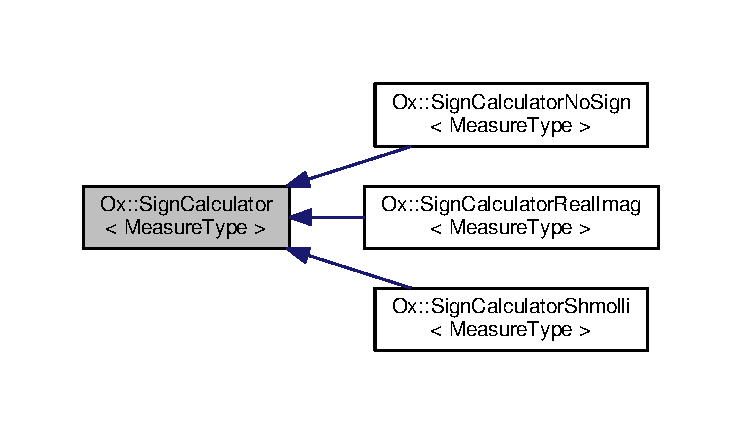
\includegraphics[width=350pt]{class_ox_1_1_sign_calculator__inherit__graph}
\end{center}
\end{figure}
\subsection*{Public Member Functions}
\begin{DoxyCompactItemize}
\item 
virtual const Measure\+Type $\ast$ {\bfseries get\+Inv\+Times} () const \hypertarget{class_ox_1_1_sign_calculator_aeae2b269b870b515f9da0ecb9a0c9dda}{}\label{class_ox_1_1_sign_calculator_aeae2b269b870b515f9da0ecb9a0c9dda}

\item 
virtual const Measure\+Type $\ast$ {\bfseries get\+Sig\+Mag} () const \hypertarget{class_ox_1_1_sign_calculator_abe5cfb287faab9e06e113bf33daa9b2e}{}\label{class_ox_1_1_sign_calculator_abe5cfb287faab9e06e113bf33daa9b2e}

\item 
virtual const Measure\+Type $\ast$ {\bfseries get\+Sig\+Pha} () const \hypertarget{class_ox_1_1_sign_calculator_a5d875d51f77739c61d8c6391d665ade9}{}\label{class_ox_1_1_sign_calculator_a5d875d51f77739c61d8c6391d665ade9}

\item 
virtual Measure\+Type $\ast$ {\bfseries get\+Signal} ()\hypertarget{class_ox_1_1_sign_calculator_ac4dc2ae5e3e5eee88d0a3a347a68a637}{}\label{class_ox_1_1_sign_calculator_ac4dc2ae5e3e5eee88d0a3a347a68a637}

\item 
virtual Measure\+Type $\ast$ {\bfseries get\+Signs} ()\hypertarget{class_ox_1_1_sign_calculator_a04d65630c95cf94ee6198193a5c0c346}{}\label{class_ox_1_1_sign_calculator_a04d65630c95cf94ee6198193a5c0c346}

\item 
virtual int {\bfseries get\+N\+Samples} ()\hypertarget{class_ox_1_1_sign_calculator_a6f1f77383cd088a1339ae91ce0b58e40}{}\label{class_ox_1_1_sign_calculator_a6f1f77383cd088a1339ae91ce0b58e40}

\item 
virtual void {\bfseries set\+Inv\+Times} (const Measure\+Type $\ast$\+\_\+\+Inv\+Times)\hypertarget{class_ox_1_1_sign_calculator_a184b9d2bd4b6677fef960aef40dbfe1c}{}\label{class_ox_1_1_sign_calculator_a184b9d2bd4b6677fef960aef40dbfe1c}

\item 
virtual void {\bfseries set\+Sig\+Mag} (const Measure\+Type $\ast$\+\_\+\+Sig\+Mag)\hypertarget{class_ox_1_1_sign_calculator_ad010dcfd41f343b7d9cad99a3c628468}{}\label{class_ox_1_1_sign_calculator_ad010dcfd41f343b7d9cad99a3c628468}

\item 
virtual void {\bfseries set\+Sig\+Pha} (const Measure\+Type $\ast$\+\_\+\+Sig\+Pha)\hypertarget{class_ox_1_1_sign_calculator_a1fe78e188915e35e8d0db885642852c9}{}\label{class_ox_1_1_sign_calculator_a1fe78e188915e35e8d0db885642852c9}

\item 
virtual void {\bfseries set\+Signal} (Measure\+Type $\ast$\+\_\+\+Signal)\hypertarget{class_ox_1_1_sign_calculator_ade6aa249b05f92357cb825065be8a203}{}\label{class_ox_1_1_sign_calculator_ade6aa249b05f92357cb825065be8a203}

\item 
virtual void {\bfseries set\+Signs} (Measure\+Type $\ast$\+\_\+\+Signs)\hypertarget{class_ox_1_1_sign_calculator_a3de14f899f64c93df9076fb837e553bf}{}\label{class_ox_1_1_sign_calculator_a3de14f899f64c93df9076fb837e553bf}

\item 
virtual void {\bfseries set\+N\+Samples} (int \+\_\+n\+Samples)\hypertarget{class_ox_1_1_sign_calculator_a8a4f3f8b94fad53d444cf6f1c1191497}{}\label{class_ox_1_1_sign_calculator_a8a4f3f8b94fad53d444cf6f1c1191497}

\item 
virtual int \hyperlink{class_ox_1_1_sign_calculator_a6a85028b70e41f6a60a5b639c468e455}{calculate\+Sign} ()=0
\item 
virtual void {\bfseries disp} ()\hypertarget{class_ox_1_1_sign_calculator_afc55176ad2a81085942e1e98242376bf}{}\label{class_ox_1_1_sign_calculator_afc55176ad2a81085942e1e98242376bf}

\item 
void \hyperlink{class_ox_1_1_sign_calculator_a59de754f72402b4cf7dc2f8766f0a1ff}{set\+All\+Pointers\+To\+Null} ()\hypertarget{class_ox_1_1_sign_calculator_a59de754f72402b4cf7dc2f8766f0a1ff}{}\label{class_ox_1_1_sign_calculator_a59de754f72402b4cf7dc2f8766f0a1ff}

\begin{DoxyCompactList}\small\item\em set all the pointers to zero \end{DoxyCompactList}\item 
\hyperlink{class_ox_1_1_sign_calculator_a1b0a177a5f2c6080d6730ff5fdc384af}{Sign\+Calculator} ()\hypertarget{class_ox_1_1_sign_calculator_a1b0a177a5f2c6080d6730ff5fdc384af}{}\label{class_ox_1_1_sign_calculator_a1b0a177a5f2c6080d6730ff5fdc384af}

\begin{DoxyCompactList}\small\item\em constructor \end{DoxyCompactList}\item 
\hyperlink{class_ox_1_1_sign_calculator_a118469032ecb643b93ba56f948fdce85}{Sign\+Calculator} (const \hyperlink{class_ox_1_1_sign_calculator}{Sign\+Calculator} \&old)\hypertarget{class_ox_1_1_sign_calculator_a118469032ecb643b93ba56f948fdce85}{}\label{class_ox_1_1_sign_calculator_a118469032ecb643b93ba56f948fdce85}

\begin{DoxyCompactList}\small\item\em copy constructor \end{DoxyCompactList}\item 
virtual \hyperlink{class_ox_1_1_sign_calculator}{Sign\+Calculator}$<$ Measure\+Type $>$ $\ast$ \hyperlink{class_ox_1_1_sign_calculator_a40d9d97a505a69b687429bf545597687}{new\+By\+Cloning} ()=0
\item 
virtual \hyperlink{class_ox_1_1_sign_calculator_a5143a172e360633d8df758756d146889}{$\sim$\+Sign\+Calculator} ()\hypertarget{class_ox_1_1_sign_calculator_a5143a172e360633d8df758756d146889}{}\label{class_ox_1_1_sign_calculator_a5143a172e360633d8df758756d146889}

\begin{DoxyCompactList}\small\item\em do not forget about the virtual destructor, see \href{https://stackoverflow.com/questions/461203/when-to-use-virtual-destructors}{\tt https\+://stackoverflow.\+com/questions/461203/when-\/to-\/use-\/virtual-\/destructors} \end{DoxyCompactList}\end{DoxyCompactItemize}
\subsection*{Protected Attributes}
\begin{DoxyCompactItemize}
\item 
const Measure\+Type $\ast$ {\bfseries \+\_\+\+Inv\+Times}\hypertarget{class_ox_1_1_sign_calculator_a46be35659f793c2e1280a975f799db4d}{}\label{class_ox_1_1_sign_calculator_a46be35659f793c2e1280a975f799db4d}

\item 
const Measure\+Type $\ast$ {\bfseries \+\_\+\+Sig\+Mag}\hypertarget{class_ox_1_1_sign_calculator_a635a62974bc9b9f30d0d560a84fcf3f1}{}\label{class_ox_1_1_sign_calculator_a635a62974bc9b9f30d0d560a84fcf3f1}

\item 
const Measure\+Type $\ast$ {\bfseries \+\_\+\+Sig\+Pha}\hypertarget{class_ox_1_1_sign_calculator_a19b203aacea5e39bc9675a27c57197d3}{}\label{class_ox_1_1_sign_calculator_a19b203aacea5e39bc9675a27c57197d3}

\item 
Measure\+Type $\ast$ {\bfseries \+\_\+\+Signal}\hypertarget{class_ox_1_1_sign_calculator_aaf53cad7c5d49133017677f8abb589bf}{}\label{class_ox_1_1_sign_calculator_aaf53cad7c5d49133017677f8abb589bf}

\item 
Measure\+Type $\ast$ {\bfseries \+\_\+\+Signs}\hypertarget{class_ox_1_1_sign_calculator_a6dda6e1e4d83dd7ad4654f7fd2b44bb3}{}\label{class_ox_1_1_sign_calculator_a6dda6e1e4d83dd7ad4654f7fd2b44bb3}

\item 
int {\bfseries \+\_\+n\+Samples}\hypertarget{class_ox_1_1_sign_calculator_a133488500068bccf0e041d9244a09e02}{}\label{class_ox_1_1_sign_calculator_a133488500068bccf0e041d9244a09e02}

\end{DoxyCompactItemize}


\subsection{Detailed Description}
\subsubsection*{template$<$typename Measure\+Type$>$\\*
class Ox\+::\+Sign\+Calculator$<$ Measure\+Type $>$}


\begin{DoxyTemplParams}{Template Parameters}
{\em Measure\+Type} & \\
\hline
\end{DoxyTemplParams}


\subsection{Member Function Documentation}
\index{Ox\+::\+Sign\+Calculator@{Ox\+::\+Sign\+Calculator}!calculate\+Sign@{calculate\+Sign}}
\index{calculate\+Sign@{calculate\+Sign}!Ox\+::\+Sign\+Calculator@{Ox\+::\+Sign\+Calculator}}
\subsubsection[{\texorpdfstring{calculate\+Sign()=0}{calculateSign()=0}}]{\setlength{\rightskip}{0pt plus 5cm}template$<$typename Measure\+Type$>$ virtual int {\bf Ox\+::\+Sign\+Calculator}$<$ Measure\+Type $>$\+::calculate\+Sign (
\begin{DoxyParamCaption}
{}
\end{DoxyParamCaption}
)\hspace{0.3cm}{\ttfamily [pure virtual]}}\hypertarget{class_ox_1_1_sign_calculator_a6a85028b70e41f6a60a5b639c468e455}{}\label{class_ox_1_1_sign_calculator_a6a85028b70e41f6a60a5b639c468e455}
the most important function of this class \begin{DoxyReturn}{Returns}
success/failure 
\end{DoxyReturn}


Implemented in \hyperlink{class_ox_1_1_sign_calculator_no_sign_a8e78a82d817f66385d1a2140f8ef11d7}{Ox\+::\+Sign\+Calculator\+No\+Sign$<$ Measure\+Type $>$}, \hyperlink{class_ox_1_1_sign_calculator_real_imag_ae3f3c8f8e8ea994da7ad56f4a180cb36}{Ox\+::\+Sign\+Calculator\+Real\+Imag$<$ Measure\+Type $>$}, and \hyperlink{class_ox_1_1_sign_calculator_shmolli_ab981a3a9790976de560609860f455edd}{Ox\+::\+Sign\+Calculator\+Shmolli$<$ Measure\+Type $>$}.

\index{Ox\+::\+Sign\+Calculator@{Ox\+::\+Sign\+Calculator}!new\+By\+Cloning@{new\+By\+Cloning}}
\index{new\+By\+Cloning@{new\+By\+Cloning}!Ox\+::\+Sign\+Calculator@{Ox\+::\+Sign\+Calculator}}
\subsubsection[{\texorpdfstring{new\+By\+Cloning()=0}{newByCloning()=0}}]{\setlength{\rightskip}{0pt plus 5cm}template$<$typename Measure\+Type$>$ virtual {\bf Sign\+Calculator}$<$Measure\+Type$>$$\ast$ {\bf Ox\+::\+Sign\+Calculator}$<$ Measure\+Type $>$\+::new\+By\+Cloning (
\begin{DoxyParamCaption}
{}
\end{DoxyParamCaption}
)\hspace{0.3cm}{\ttfamily [pure virtual]}}\hypertarget{class_ox_1_1_sign_calculator_a40d9d97a505a69b687429bf545597687}{}\label{class_ox_1_1_sign_calculator_a40d9d97a505a69b687429bf545597687}
cloning \begin{DoxyReturn}{Returns}

\end{DoxyReturn}


Implemented in \hyperlink{class_ox_1_1_sign_calculator_shmolli_a9d9cd9b7107e43b4762846f54ff023d4}{Ox\+::\+Sign\+Calculator\+Shmolli$<$ Measure\+Type $>$}, \hyperlink{class_ox_1_1_sign_calculator_no_sign_ac480086ad668ac264393b1b18a926221}{Ox\+::\+Sign\+Calculator\+No\+Sign$<$ Measure\+Type $>$}, and \hyperlink{class_ox_1_1_sign_calculator_real_imag_ae3340d1ac5728efcaf3d5a9299f01f2c}{Ox\+::\+Sign\+Calculator\+Real\+Imag$<$ Measure\+Type $>$}.



The documentation for this class was generated from the following file\+:\begin{DoxyCompactItemize}
\item 
lib/\hyperlink{_ox_sign_calculator_8h}{Ox\+Sign\+Calculator.\+h}\end{DoxyCompactItemize}

\hypertarget{class_ox_1_1_sign_calculator_no_sign}{}\section{Ox\+:\+:Sign\+Calculator\+No\+Sign$<$ Measure\+Type $>$ Class Template Reference}
\label{class_ox_1_1_sign_calculator_no_sign}\index{Ox\+::\+Sign\+Calculator\+No\+Sign$<$ Measure\+Type $>$@{Ox\+::\+Sign\+Calculator\+No\+Sign$<$ Measure\+Type $>$}}


{\ttfamily \#include $<$Ox\+Sign\+Calculator\+No\+Sign.\+h$>$}



Inheritance diagram for Ox\+:\+:Sign\+Calculator\+No\+Sign$<$ Measure\+Type $>$\+:
\nopagebreak
\begin{figure}[H]
\begin{center}
\leavevmode
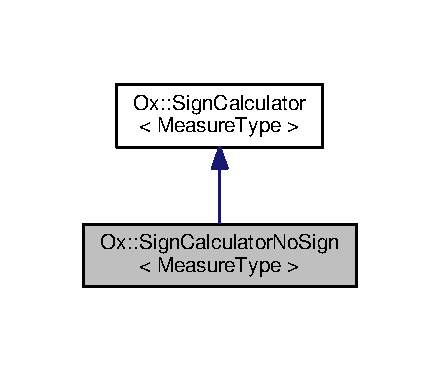
\includegraphics[width=211pt]{class_ox_1_1_sign_calculator_no_sign__inherit__graph}
\end{center}
\end{figure}


Collaboration diagram for Ox\+:\+:Sign\+Calculator\+No\+Sign$<$ Measure\+Type $>$\+:
\nopagebreak
\begin{figure}[H]
\begin{center}
\leavevmode
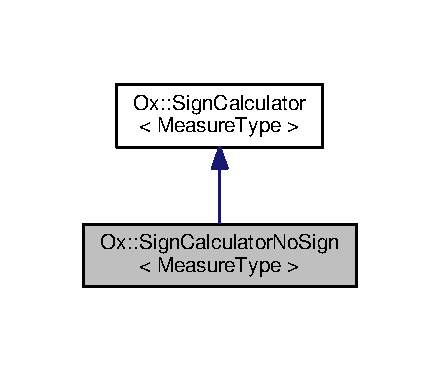
\includegraphics[width=211pt]{class_ox_1_1_sign_calculator_no_sign__coll__graph}
\end{center}
\end{figure}
\subsection*{Public Member Functions}
\begin{DoxyCompactItemize}
\item 
virtual int \hyperlink{class_ox_1_1_sign_calculator_no_sign_a8e78a82d817f66385d1a2140f8ef11d7}{calculate\+Sign} ()
\item 
\hyperlink{class_ox_1_1_sign_calculator_no_sign_ad61e381c257ac4b4f615d94461dc49b1}{Sign\+Calculator\+No\+Sign} ()\hypertarget{class_ox_1_1_sign_calculator_no_sign_ad61e381c257ac4b4f615d94461dc49b1}{}\label{class_ox_1_1_sign_calculator_no_sign_ad61e381c257ac4b4f615d94461dc49b1}

\begin{DoxyCompactList}\small\item\em constructor \end{DoxyCompactList}\item 
\hyperlink{class_ox_1_1_sign_calculator_no_sign_af7d02fdbe8062421741d00f60c9e57aa}{Sign\+Calculator\+No\+Sign} (const \hyperlink{class_ox_1_1_sign_calculator_no_sign}{Sign\+Calculator\+No\+Sign} \&old)\hypertarget{class_ox_1_1_sign_calculator_no_sign_af7d02fdbe8062421741d00f60c9e57aa}{}\label{class_ox_1_1_sign_calculator_no_sign_af7d02fdbe8062421741d00f60c9e57aa}

\begin{DoxyCompactList}\small\item\em copy constructor \end{DoxyCompactList}\item 
virtual \hyperlink{class_ox_1_1_sign_calculator}{Sign\+Calculator}$<$ Measure\+Type $>$ $\ast$ \hyperlink{class_ox_1_1_sign_calculator_no_sign_ac480086ad668ac264393b1b18a926221}{new\+By\+Cloning} ()
\item 
virtual \hyperlink{class_ox_1_1_sign_calculator_no_sign_a1da2b6c351daf89811c6d9618df2bb74}{$\sim$\+Sign\+Calculator\+No\+Sign} ()\hypertarget{class_ox_1_1_sign_calculator_no_sign_a1da2b6c351daf89811c6d9618df2bb74}{}\label{class_ox_1_1_sign_calculator_no_sign_a1da2b6c351daf89811c6d9618df2bb74}

\begin{DoxyCompactList}\small\item\em do not forget about the virtual destructor, see \href{https://stackoverflow.com/questions/461203/when-to-use-virtual-destructors}{\tt https\+://stackoverflow.\+com/questions/461203/when-\/to-\/use-\/virtual-\/destructors} \end{DoxyCompactList}\end{DoxyCompactItemize}
\subsection*{Additional Inherited Members}


\subsection{Detailed Description}
\subsubsection*{template$<$typename Measure\+Type$>$\\*
class Ox\+::\+Sign\+Calculator\+No\+Sign$<$ Measure\+Type $>$}


\begin{DoxyTemplParams}{Template Parameters}
{\em Measure\+Type} & \\
\hline
\end{DoxyTemplParams}


\subsection{Member Function Documentation}
\index{Ox\+::\+Sign\+Calculator\+No\+Sign@{Ox\+::\+Sign\+Calculator\+No\+Sign}!calculate\+Sign@{calculate\+Sign}}
\index{calculate\+Sign@{calculate\+Sign}!Ox\+::\+Sign\+Calculator\+No\+Sign@{Ox\+::\+Sign\+Calculator\+No\+Sign}}
\subsubsection[{\texorpdfstring{calculate\+Sign()}{calculateSign()}}]{\setlength{\rightskip}{0pt plus 5cm}template$<$typename Measure\+Type$>$ virtual int {\bf Ox\+::\+Sign\+Calculator\+No\+Sign}$<$ Measure\+Type $>$\+::calculate\+Sign (
\begin{DoxyParamCaption}
{}
\end{DoxyParamCaption}
)\hspace{0.3cm}{\ttfamily [inline]}, {\ttfamily [virtual]}}\hypertarget{class_ox_1_1_sign_calculator_no_sign_a8e78a82d817f66385d1a2140f8ef11d7}{}\label{class_ox_1_1_sign_calculator_no_sign_a8e78a82d817f66385d1a2140f8ef11d7}
the most important function of this class \begin{DoxyReturn}{Returns}
success/failure 
\end{DoxyReturn}


Implements \hyperlink{class_ox_1_1_sign_calculator_a6a85028b70e41f6a60a5b639c468e455}{Ox\+::\+Sign\+Calculator$<$ Measure\+Type $>$}.

\index{Ox\+::\+Sign\+Calculator\+No\+Sign@{Ox\+::\+Sign\+Calculator\+No\+Sign}!new\+By\+Cloning@{new\+By\+Cloning}}
\index{new\+By\+Cloning@{new\+By\+Cloning}!Ox\+::\+Sign\+Calculator\+No\+Sign@{Ox\+::\+Sign\+Calculator\+No\+Sign}}
\subsubsection[{\texorpdfstring{new\+By\+Cloning()}{newByCloning()}}]{\setlength{\rightskip}{0pt plus 5cm}template$<$typename Measure\+Type$>$ virtual {\bf Sign\+Calculator}$<$Measure\+Type$>$$\ast$ {\bf Ox\+::\+Sign\+Calculator\+No\+Sign}$<$ Measure\+Type $>$\+::new\+By\+Cloning (
\begin{DoxyParamCaption}
{}
\end{DoxyParamCaption}
)\hspace{0.3cm}{\ttfamily [inline]}, {\ttfamily [virtual]}}\hypertarget{class_ox_1_1_sign_calculator_no_sign_ac480086ad668ac264393b1b18a926221}{}\label{class_ox_1_1_sign_calculator_no_sign_ac480086ad668ac264393b1b18a926221}
cloning \begin{DoxyReturn}{Returns}

\end{DoxyReturn}


Implements \hyperlink{class_ox_1_1_sign_calculator_a40d9d97a505a69b687429bf545597687}{Ox\+::\+Sign\+Calculator$<$ Measure\+Type $>$}.



The documentation for this class was generated from the following file\+:\begin{DoxyCompactItemize}
\item 
lib/\hyperlink{_ox_sign_calculator_no_sign_8h}{Ox\+Sign\+Calculator\+No\+Sign.\+h}\end{DoxyCompactItemize}

\hypertarget{class_ox_1_1_sign_calculator_real_imag}{}\section{Ox\+:\+:Sign\+Calculator\+Real\+Imag$<$ Measure\+Type $>$ Class Template Reference}
\label{class_ox_1_1_sign_calculator_real_imag}\index{Ox\+::\+Sign\+Calculator\+Real\+Imag$<$ Measure\+Type $>$@{Ox\+::\+Sign\+Calculator\+Real\+Imag$<$ Measure\+Type $>$}}


{\ttfamily \#include $<$Ox\+Sign\+Calculator\+Real\+Imag.\+h$>$}



Inheritance diagram for Ox\+:\+:Sign\+Calculator\+Real\+Imag$<$ Measure\+Type $>$\+:
\nopagebreak
\begin{figure}[H]
\begin{center}
\leavevmode
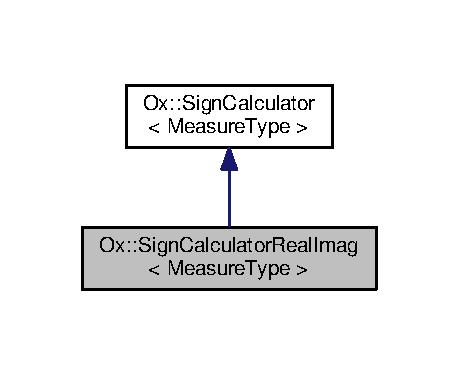
\includegraphics[width=221pt]{class_ox_1_1_sign_calculator_real_imag__inherit__graph}
\end{center}
\end{figure}


Collaboration diagram for Ox\+:\+:Sign\+Calculator\+Real\+Imag$<$ Measure\+Type $>$\+:
\nopagebreak
\begin{figure}[H]
\begin{center}
\leavevmode
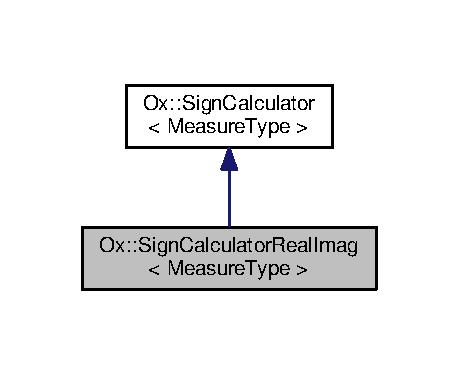
\includegraphics[width=221pt]{class_ox_1_1_sign_calculator_real_imag__coll__graph}
\end{center}
\end{figure}
\subsection*{Public Member Functions}
\begin{DoxyCompactItemize}
\item 
virtual int \hyperlink{class_ox_1_1_sign_calculator_real_imag_ae3f3c8f8e8ea994da7ad56f4a180cb36}{calculate\+Sign} ()
\item 
virtual \hyperlink{class_ox_1_1_sign_calculator}{Sign\+Calculator}$<$ Measure\+Type $>$ $\ast$ \hyperlink{class_ox_1_1_sign_calculator_real_imag_ae3340d1ac5728efcaf3d5a9299f01f2c}{new\+By\+Cloning} ()
\end{DoxyCompactItemize}
\subsection*{Static Public Member Functions}
\begin{DoxyCompactItemize}
\item 
static int {\bfseries Real\+Mag\+Phase2\+Signs} (int n\+Samples, const Measure\+Type $\ast$sig\+Mag, const Measure\+Type $\ast$sig\+Pha, Measure\+Type $\ast$signal, Measure\+Type $\ast$signs)\hypertarget{class_ox_1_1_sign_calculator_real_imag_a916a7be502489b814bd3b147075ae31d}{}\label{class_ox_1_1_sign_calculator_real_imag_a916a7be502489b814bd3b147075ae31d}

\end{DoxyCompactItemize}
\subsection*{Additional Inherited Members}


\subsection{Detailed Description}
\subsubsection*{template$<$typename Measure\+Type$>$\\*
class Ox\+::\+Sign\+Calculator\+Real\+Imag$<$ Measure\+Type $>$}


\begin{DoxyTemplParams}{Template Parameters}
{\em Measure\+Type} & \\
\hline
\end{DoxyTemplParams}


\subsection{Member Function Documentation}
\index{Ox\+::\+Sign\+Calculator\+Real\+Imag@{Ox\+::\+Sign\+Calculator\+Real\+Imag}!calculate\+Sign@{calculate\+Sign}}
\index{calculate\+Sign@{calculate\+Sign}!Ox\+::\+Sign\+Calculator\+Real\+Imag@{Ox\+::\+Sign\+Calculator\+Real\+Imag}}
\subsubsection[{\texorpdfstring{calculate\+Sign()}{calculateSign()}}]{\setlength{\rightskip}{0pt plus 5cm}template$<$typename Measure\+Type$>$ virtual int {\bf Ox\+::\+Sign\+Calculator\+Real\+Imag}$<$ Measure\+Type $>$\+::calculate\+Sign (
\begin{DoxyParamCaption}
{}
\end{DoxyParamCaption}
)\hspace{0.3cm}{\ttfamily [inline]}, {\ttfamily [virtual]}}\hypertarget{class_ox_1_1_sign_calculator_real_imag_ae3f3c8f8e8ea994da7ad56f4a180cb36}{}\label{class_ox_1_1_sign_calculator_real_imag_ae3f3c8f8e8ea994da7ad56f4a180cb36}
the most important function of this class \begin{DoxyReturn}{Returns}
success/failure 
\end{DoxyReturn}


Implements \hyperlink{class_ox_1_1_sign_calculator_a6a85028b70e41f6a60a5b639c468e455}{Ox\+::\+Sign\+Calculator$<$ Measure\+Type $>$}.

\index{Ox\+::\+Sign\+Calculator\+Real\+Imag@{Ox\+::\+Sign\+Calculator\+Real\+Imag}!new\+By\+Cloning@{new\+By\+Cloning}}
\index{new\+By\+Cloning@{new\+By\+Cloning}!Ox\+::\+Sign\+Calculator\+Real\+Imag@{Ox\+::\+Sign\+Calculator\+Real\+Imag}}
\subsubsection[{\texorpdfstring{new\+By\+Cloning()}{newByCloning()}}]{\setlength{\rightskip}{0pt plus 5cm}template$<$typename Measure\+Type$>$ virtual {\bf Sign\+Calculator}$<$Measure\+Type$>$$\ast$ {\bf Ox\+::\+Sign\+Calculator\+Real\+Imag}$<$ Measure\+Type $>$\+::new\+By\+Cloning (
\begin{DoxyParamCaption}
{}
\end{DoxyParamCaption}
)\hspace{0.3cm}{\ttfamily [inline]}, {\ttfamily [virtual]}}\hypertarget{class_ox_1_1_sign_calculator_real_imag_ae3340d1ac5728efcaf3d5a9299f01f2c}{}\label{class_ox_1_1_sign_calculator_real_imag_ae3340d1ac5728efcaf3d5a9299f01f2c}
cloning \begin{DoxyReturn}{Returns}

\end{DoxyReturn}


Implements \hyperlink{class_ox_1_1_sign_calculator_a40d9d97a505a69b687429bf545597687}{Ox\+::\+Sign\+Calculator$<$ Measure\+Type $>$}.



The documentation for this class was generated from the following file\+:\begin{DoxyCompactItemize}
\item 
lib/\hyperlink{_ox_sign_calculator_real_imag_8h}{Ox\+Sign\+Calculator\+Real\+Imag.\+h}\end{DoxyCompactItemize}

\hypertarget{class_ox_1_1_sign_calculator_shmolli}{\section{Ox\-:\-:Sign\-Calculator\-Shmolli$<$ Measure\-Type $>$ Class Template Reference}
\label{class_ox_1_1_sign_calculator_shmolli}\index{Ox\-::\-Sign\-Calculator\-Shmolli$<$ Measure\-Type $>$@{Ox\-::\-Sign\-Calculator\-Shmolli$<$ Measure\-Type $>$}}
}


{\ttfamily \#include $<$Ox\-Sign\-Calculator\-Shmolli.\-h$>$}



Inheritance diagram for Ox\-:\-:Sign\-Calculator\-Shmolli$<$ Measure\-Type $>$\-:
\nopagebreak
\begin{figure}[H]
\begin{center}
\leavevmode
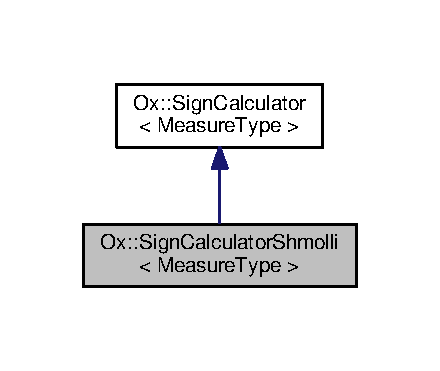
\includegraphics[width=210pt]{class_ox_1_1_sign_calculator_shmolli__inherit__graph}
\end{center}
\end{figure}


Collaboration diagram for Ox\-:\-:Sign\-Calculator\-Shmolli$<$ Measure\-Type $>$\-:
\nopagebreak
\begin{figure}[H]
\begin{center}
\leavevmode
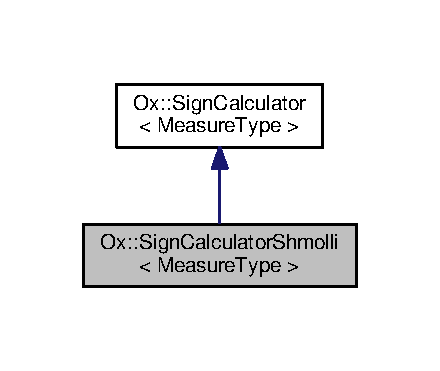
\includegraphics[width=210pt]{class_ox_1_1_sign_calculator_shmolli__coll__graph}
\end{center}
\end{figure}
\subsection*{Public Member Functions}
\begin{DoxyCompactItemize}
\item 
virtual int \hyperlink{class_ox_1_1_sign_calculator_shmolli_ab981a3a9790976de560609860f455edd}{calculate\-Sign} ()
\item 
\hypertarget{class_ox_1_1_sign_calculator_shmolli_af1182129716f5b952023280e61838a52}{virtual int {\bfseries get\-Pha\-Min} ()}\label{class_ox_1_1_sign_calculator_shmolli_af1182129716f5b952023280e61838a52}

\item 
\hypertarget{class_ox_1_1_sign_calculator_shmolli_afa6d41a49c0a321100164ae203904496}{virtual int {\bfseries get\-Pha\-Max} ()}\label{class_ox_1_1_sign_calculator_shmolli_afa6d41a49c0a321100164ae203904496}

\item 
\hypertarget{class_ox_1_1_sign_calculator_shmolli_aacfc207842127c87086f5595b9188acd}{virtual void {\bfseries set\-Pha\-Min} (int \-\_\-pha\-Min)}\label{class_ox_1_1_sign_calculator_shmolli_aacfc207842127c87086f5595b9188acd}

\item 
\hypertarget{class_ox_1_1_sign_calculator_shmolli_a3ec4977cf59bff37f95aa3fb1da1ae24}{virtual void {\bfseries set\-Pha\-Max} (int \-\_\-pha\-Max)}\label{class_ox_1_1_sign_calculator_shmolli_a3ec4977cf59bff37f95aa3fb1da1ae24}

\item 
\hypertarget{class_ox_1_1_sign_calculator_shmolli_a6ecfab9fb03fec0e62ad4951d5ab6c1b}{\hyperlink{class_ox_1_1_sign_calculator_shmolli_a6ecfab9fb03fec0e62ad4951d5ab6c1b}{Sign\-Calculator\-Shmolli} ()}\label{class_ox_1_1_sign_calculator_shmolli_a6ecfab9fb03fec0e62ad4951d5ab6c1b}

\begin{DoxyCompactList}\small\item\em constructor \end{DoxyCompactList}\item 
\hypertarget{class_ox_1_1_sign_calculator_shmolli_ae5b6751ae99992cc2075f0dc4b729605}{\hyperlink{class_ox_1_1_sign_calculator_shmolli_ae5b6751ae99992cc2075f0dc4b729605}{Sign\-Calculator\-Shmolli} (const \hyperlink{class_ox_1_1_sign_calculator_shmolli}{Sign\-Calculator\-Shmolli} \&old)}\label{class_ox_1_1_sign_calculator_shmolli_ae5b6751ae99992cc2075f0dc4b729605}

\begin{DoxyCompactList}\small\item\em copy constructor \end{DoxyCompactList}\item 
virtual \hyperlink{class_ox_1_1_sign_calculator}{Sign\-Calculator}\\*
$<$ Measure\-Type $>$ $\ast$ \hyperlink{class_ox_1_1_sign_calculator_shmolli_a9d9cd9b7107e43b4762846f54ff023d4}{new\-By\-Cloning} ()
\end{DoxyCompactItemize}
\subsection*{Static Public Member Functions}
\begin{DoxyCompactItemize}
\item 
static int \hyperlink{class_ox_1_1_sign_calculator_shmolli_a281487db14afd7142d0a9439fd8d319d}{S\-K\-P\-Phase2\-Signs} (int n\-Samples, const Measure\-Type $\ast$inv\-Times, const Measure\-Type $\ast$sig\-Mag, const Measure\-Type $\ast$sig\-Pha, Measure\-Type $\ast$signal, Measure\-Type $\ast$signs, Measure\-Type pha\-Min, Measure\-Type pha\-Max)
\end{DoxyCompactItemize}
\subsection*{Protected Attributes}
\begin{DoxyCompactItemize}
\item 
\hypertarget{class_ox_1_1_sign_calculator_shmolli_a3384cfa4793a5a6e9e6285d70b3131be}{double {\bfseries \-\_\-pha\-Min}}\label{class_ox_1_1_sign_calculator_shmolli_a3384cfa4793a5a6e9e6285d70b3131be}

\item 
\hypertarget{class_ox_1_1_sign_calculator_shmolli_a1b17399c7a9c9a30dd2fcb9a09db3ae8}{double {\bfseries \-\_\-pha\-Max}}\label{class_ox_1_1_sign_calculator_shmolli_a1b17399c7a9c9a30dd2fcb9a09db3ae8}

\end{DoxyCompactItemize}
\subsection*{Static Protected Attributes}
\begin{DoxyCompactItemize}
\item 
\hypertarget{class_ox_1_1_sign_calculator_shmolli_a885834272c7d64afc5faae54fce33e8b}{static const int {\bfseries M\-A\-X\-\_\-\-M\-O\-L\-L\-I\-\_\-\-T\-I\-\_\-\-S\-A\-M\-P\-L\-E\-S} = 128}\label{class_ox_1_1_sign_calculator_shmolli_a885834272c7d64afc5faae54fce33e8b}

\item 
\hypertarget{class_ox_1_1_sign_calculator_shmolli_a6540643a5e432b753b631a5abc7b0619}{static const int {\bfseries M\-A\-X\-\_\-\-T1\-\_\-\-T\-R\-E\-S\-H\-O\-L\-D} = 4000}\label{class_ox_1_1_sign_calculator_shmolli_a6540643a5e432b753b631a5abc7b0619}

\end{DoxyCompactItemize}


\subsection{Detailed Description}
\subsubsection*{template$<$typename Measure\-Type$>$class Ox\-::\-Sign\-Calculator\-Shmolli$<$ Measure\-Type $>$}


\begin{DoxyTemplParams}{Template Parameters}
{\em Measure\-Type} & \\
\hline
\end{DoxyTemplParams}


\subsection{Member Function Documentation}
\hypertarget{class_ox_1_1_sign_calculator_shmolli_ab981a3a9790976de560609860f455edd}{\index{Ox\-::\-Sign\-Calculator\-Shmolli@{Ox\-::\-Sign\-Calculator\-Shmolli}!calculate\-Sign@{calculate\-Sign}}
\index{calculate\-Sign@{calculate\-Sign}!Ox::SignCalculatorShmolli@{Ox\-::\-Sign\-Calculator\-Shmolli}}
\subsubsection[{calculate\-Sign}]{\setlength{\rightskip}{0pt plus 5cm}template$<$typename Measure\-Type$>$ virtual int {\bf Ox\-::\-Sign\-Calculator\-Shmolli}$<$ Measure\-Type $>$\-::calculate\-Sign (
\begin{DoxyParamCaption}
{}
\end{DoxyParamCaption}
)\hspace{0.3cm}{\ttfamily [inline]}, {\ttfamily [virtual]}}}\label{class_ox_1_1_sign_calculator_shmolli_ab981a3a9790976de560609860f455edd}
the most important function of this class \begin{DoxyReturn}{Returns}
success/failure 
\end{DoxyReturn}


Implements \hyperlink{class_ox_1_1_sign_calculator_a6a85028b70e41f6a60a5b639c468e455}{Ox\-::\-Sign\-Calculator$<$ Measure\-Type $>$}.

\hypertarget{class_ox_1_1_sign_calculator_shmolli_a9d9cd9b7107e43b4762846f54ff023d4}{\index{Ox\-::\-Sign\-Calculator\-Shmolli@{Ox\-::\-Sign\-Calculator\-Shmolli}!new\-By\-Cloning@{new\-By\-Cloning}}
\index{new\-By\-Cloning@{new\-By\-Cloning}!Ox::SignCalculatorShmolli@{Ox\-::\-Sign\-Calculator\-Shmolli}}
\subsubsection[{new\-By\-Cloning}]{\setlength{\rightskip}{0pt plus 5cm}template$<$typename Measure\-Type$>$ virtual {\bf Sign\-Calculator}$<$Measure\-Type$>$$\ast$ {\bf Ox\-::\-Sign\-Calculator\-Shmolli}$<$ Measure\-Type $>$\-::new\-By\-Cloning (
\begin{DoxyParamCaption}
{}
\end{DoxyParamCaption}
)\hspace{0.3cm}{\ttfamily [inline]}, {\ttfamily [virtual]}}}\label{class_ox_1_1_sign_calculator_shmolli_a9d9cd9b7107e43b4762846f54ff023d4}
cloning \begin{DoxyReturn}{Returns}

\end{DoxyReturn}


Implements \hyperlink{class_ox_1_1_sign_calculator_a40d9d97a505a69b687429bf545597687}{Ox\-::\-Sign\-Calculator$<$ Measure\-Type $>$}.

\hypertarget{class_ox_1_1_sign_calculator_shmolli_a281487db14afd7142d0a9439fd8d319d}{\index{Ox\-::\-Sign\-Calculator\-Shmolli@{Ox\-::\-Sign\-Calculator\-Shmolli}!S\-K\-P\-Phase2\-Signs@{S\-K\-P\-Phase2\-Signs}}
\index{S\-K\-P\-Phase2\-Signs@{S\-K\-P\-Phase2\-Signs}!Ox::SignCalculatorShmolli@{Ox\-::\-Sign\-Calculator\-Shmolli}}
\subsubsection[{S\-K\-P\-Phase2\-Signs}]{\setlength{\rightskip}{0pt plus 5cm}template$<$typename Measure\-Type $>$ int {\bf Ox\-::\-Sign\-Calculator\-Shmolli}$<$ Measure\-Type $>$\-::S\-K\-P\-Phase2\-Signs (
\begin{DoxyParamCaption}
\item[{int}]{n\-Samples, }
\item[{const Measure\-Type $\ast$}]{inv\-Times, }
\item[{const Measure\-Type $\ast$}]{sig\-Mag, }
\item[{const Measure\-Type $\ast$}]{sig\-Pha, }
\item[{Measure\-Type $\ast$}]{signal, }
\item[{Measure\-Type $\ast$}]{signs, }
\item[{Measure\-Type}]{pha\-Min, }
\item[{Measure\-Type}]{pha\-Max}
\end{DoxyParamCaption}
)\hspace{0.3cm}{\ttfamily [static]}}}\label{class_ox_1_1_sign_calculator_shmolli_a281487db14afd7142d0a9439fd8d319d}
more complicated. 

The documentation for this class was generated from the following file\-:\begin{DoxyCompactItemize}
\item 
lib/\hyperlink{_ox_sign_calculator_shmolli_8h}{Ox\-Sign\-Calculator\-Shmolli.\-h}\end{DoxyCompactItemize}

\hypertarget{class_ox_1_1_start_point_calculator}{}\section{Ox\+:\+:Start\+Point\+Calculator$<$ Measure\+Type $>$ Class Template Reference}
\label{class_ox_1_1_start_point_calculator}\index{Ox\+::\+Start\+Point\+Calculator$<$ Measure\+Type $>$@{Ox\+::\+Start\+Point\+Calculator$<$ Measure\+Type $>$}}


{\ttfamily \#include $<$Ox\+Start\+Point\+Calculator.\+h$>$}



Inheritance diagram for Ox\+:\+:Start\+Point\+Calculator$<$ Measure\+Type $>$\+:
\nopagebreak
\begin{figure}[H]
\begin{center}
\leavevmode
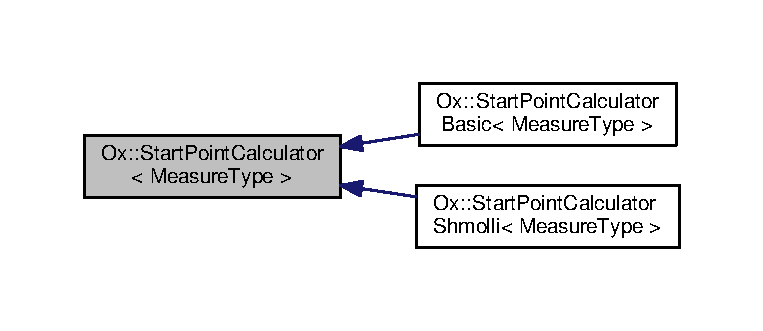
\includegraphics[width=350pt]{class_ox_1_1_start_point_calculator__inherit__graph}
\end{center}
\end{figure}
\subsection*{Public Member Functions}
\begin{DoxyCompactItemize}
\item 
virtual int \hyperlink{class_ox_1_1_start_point_calculator_a9d1132410d68eb16f3f71ec4015c0b2f}{calculate\+Start\+Point} ()=0
\item 
const Measure\+Type $\ast$ {\bfseries get\+Input\+Start\+Point} () const \hypertarget{class_ox_1_1_start_point_calculator_a01bcfb382bec0c4c28ae2bb5783b458c}{}\label{class_ox_1_1_start_point_calculator_a01bcfb382bec0c4c28ae2bb5783b458c}

\item 
Measure\+Type $\ast$ {\bfseries get\+Calculated\+Start\+Point} () const \hypertarget{class_ox_1_1_start_point_calculator_a48b39c1d6bb733821f7297593e424728}{}\label{class_ox_1_1_start_point_calculator_a48b39c1d6bb733821f7297593e424728}

\item 
int {\bfseries get\+N\+Dims} () const \hypertarget{class_ox_1_1_start_point_calculator_a75c73487e21a0f4920762c1efc96d573}{}\label{class_ox_1_1_start_point_calculator_a75c73487e21a0f4920762c1efc96d573}

\item 
virtual void {\bfseries set\+Input\+Start\+Point} (const Measure\+Type $\ast$\+\_\+\+Input\+Start\+Point)\hypertarget{class_ox_1_1_start_point_calculator_ac76047ce4b0d474203cae066471cce61}{}\label{class_ox_1_1_start_point_calculator_ac76047ce4b0d474203cae066471cce61}

\item 
virtual void {\bfseries set\+N\+Dims} (int \+\_\+n\+Dims)\hypertarget{class_ox_1_1_start_point_calculator_a02b51af6d6019cfc47d04b752ad96c86}{}\label{class_ox_1_1_start_point_calculator_a02b51af6d6019cfc47d04b752ad96c86}

\item 
virtual void {\bfseries set\+Inv\+Times} (const Measure\+Type $\ast$\+\_\+\+Inv\+Times)\hypertarget{class_ox_1_1_start_point_calculator_a0632bd0dcf7707930058d63e2176fc7a}{}\label{class_ox_1_1_start_point_calculator_a0632bd0dcf7707930058d63e2176fc7a}

\item 
virtual void {\bfseries set\+Echo\+Times} (const Measure\+Type $\ast$\+\_\+\+Echo\+Times)\hypertarget{class_ox_1_1_start_point_calculator_ab49fe45a4ee7b415edd0948c9fc76fbb}{}\label{class_ox_1_1_start_point_calculator_ab49fe45a4ee7b415edd0948c9fc76fbb}

\item 
virtual void {\bfseries set\+Sig\+Mag} (const Measure\+Type $\ast$\+\_\+\+Sig\+Mag)\hypertarget{class_ox_1_1_start_point_calculator_a7cff5323e92bc00fdc9baa2a3eef7a37}{}\label{class_ox_1_1_start_point_calculator_a7cff5323e92bc00fdc9baa2a3eef7a37}

\item 
virtual void {\bfseries set\+Signs} (const Measure\+Type $\ast$\+\_\+\+Signs)\hypertarget{class_ox_1_1_start_point_calculator_a1245375d6cad369f18ab4a32ddb28446}{}\label{class_ox_1_1_start_point_calculator_a1245375d6cad369f18ab4a32ddb28446}

\item 
virtual void {\bfseries set\+Calculated\+Start\+Point} (Measure\+Type $\ast$\+\_\+\+Calculated\+Start\+Point)\hypertarget{class_ox_1_1_start_point_calculator_aebb0511e802eff920369dec99b6c00fb}{}\label{class_ox_1_1_start_point_calculator_aebb0511e802eff920369dec99b6c00fb}

\item 
virtual void {\bfseries set\+N\+Samples} (int \+\_\+n\+Samples)\hypertarget{class_ox_1_1_start_point_calculator_a72195ac7840734cd9001d0303ab859f4}{}\label{class_ox_1_1_start_point_calculator_a72195ac7840734cd9001d0303ab859f4}

\item 
void {\bfseries disp} ()\hypertarget{class_ox_1_1_start_point_calculator_a1e68d3a23cee006d4dbdd47583c5d316}{}\label{class_ox_1_1_start_point_calculator_a1e68d3a23cee006d4dbdd47583c5d316}

\item 
void \hyperlink{class_ox_1_1_start_point_calculator_a00a48e8845623b57e414380924a3f82b}{set\+All\+Pointers\+To\+Null} ()\hypertarget{class_ox_1_1_start_point_calculator_a00a48e8845623b57e414380924a3f82b}{}\label{class_ox_1_1_start_point_calculator_a00a48e8845623b57e414380924a3f82b}

\begin{DoxyCompactList}\small\item\em set all the pointers to zero \end{DoxyCompactList}\item 
\hyperlink{class_ox_1_1_start_point_calculator_a408ce85b6fbf0ee69f4eca3176b814d6}{Start\+Point\+Calculator} ()\hypertarget{class_ox_1_1_start_point_calculator_a408ce85b6fbf0ee69f4eca3176b814d6}{}\label{class_ox_1_1_start_point_calculator_a408ce85b6fbf0ee69f4eca3176b814d6}

\begin{DoxyCompactList}\small\item\em constructor \end{DoxyCompactList}\item 
\hyperlink{class_ox_1_1_start_point_calculator_ab6b12ed8fa6b47b3335b5c7a92b94623}{Start\+Point\+Calculator} (const \hyperlink{class_ox_1_1_start_point_calculator}{Start\+Point\+Calculator} \&old)\hypertarget{class_ox_1_1_start_point_calculator_ab6b12ed8fa6b47b3335b5c7a92b94623}{}\label{class_ox_1_1_start_point_calculator_ab6b12ed8fa6b47b3335b5c7a92b94623}

\begin{DoxyCompactList}\small\item\em copy constructor \end{DoxyCompactList}\item 
virtual \hyperlink{class_ox_1_1_start_point_calculator}{Start\+Point\+Calculator}$<$ Measure\+Type $>$ $\ast$ \hyperlink{class_ox_1_1_start_point_calculator_acd2a221872002157f232e1e7f73a1859}{new\+By\+Cloning} ()=0
\item 
virtual \hyperlink{class_ox_1_1_start_point_calculator_a210c3312a8926b750dba8e498c6b620a}{$\sim$\+Start\+Point\+Calculator} ()\hypertarget{class_ox_1_1_start_point_calculator_a210c3312a8926b750dba8e498c6b620a}{}\label{class_ox_1_1_start_point_calculator_a210c3312a8926b750dba8e498c6b620a}

\begin{DoxyCompactList}\small\item\em do not forget about the virtual destructor, see \href{https://stackoverflow.com/questions/461203/when-to-use-virtual-destructors}{\tt https\+://stackoverflow.\+com/questions/461203/when-\/to-\/use-\/virtual-\/destructors} \end{DoxyCompactList}\end{DoxyCompactItemize}
\subsection*{Protected Attributes}
\begin{DoxyCompactItemize}
\item 
Measure\+Type $\ast$ {\bfseries \+\_\+\+Input\+Start\+Point}\hypertarget{class_ox_1_1_start_point_calculator_a92176ada269bb53017ed3cbedb3b629d}{}\label{class_ox_1_1_start_point_calculator_a92176ada269bb53017ed3cbedb3b629d}

\item 
Measure\+Type $\ast$ {\bfseries \+\_\+\+Calculated\+Start\+Point}\hypertarget{class_ox_1_1_start_point_calculator_a90c26143db22a371533de08a87cdada0}{}\label{class_ox_1_1_start_point_calculator_a90c26143db22a371533de08a87cdada0}

\item 
const Measure\+Type $\ast$ {\bfseries \+\_\+\+Inv\+Times}\hypertarget{class_ox_1_1_start_point_calculator_a64929ca24726ddf99017b6f18cc03e29}{}\label{class_ox_1_1_start_point_calculator_a64929ca24726ddf99017b6f18cc03e29}

\item 
const Measure\+Type $\ast$ {\bfseries \+\_\+\+Echo\+Times}\hypertarget{class_ox_1_1_start_point_calculator_a7549a2a735665d8b204c230c817fc5d4}{}\label{class_ox_1_1_start_point_calculator_a7549a2a735665d8b204c230c817fc5d4}

\item 
const Measure\+Type $\ast$ {\bfseries \+\_\+\+Sig\+Mag}\hypertarget{class_ox_1_1_start_point_calculator_a5cf615178da5bb3af984eea616548e05}{}\label{class_ox_1_1_start_point_calculator_a5cf615178da5bb3af984eea616548e05}

\item 
const Measure\+Type $\ast$ {\bfseries \+\_\+\+Signs}\hypertarget{class_ox_1_1_start_point_calculator_abce7ef554368d8739ac27dddb63382df}{}\label{class_ox_1_1_start_point_calculator_abce7ef554368d8739ac27dddb63382df}

\item 
int {\bfseries \+\_\+n\+Samples}\hypertarget{class_ox_1_1_start_point_calculator_a17601c059cd679301597bc897e297c2f}{}\label{class_ox_1_1_start_point_calculator_a17601c059cd679301597bc897e297c2f}

\item 
int {\bfseries \+\_\+n\+Dims}\hypertarget{class_ox_1_1_start_point_calculator_a1bee9378aff7741838dad45ff6d5dc1d}{}\label{class_ox_1_1_start_point_calculator_a1bee9378aff7741838dad45ff6d5dc1d}

\item 
bool {\bfseries \+\_\+n\+Dims\+Changed}\hypertarget{class_ox_1_1_start_point_calculator_a800e7f49b7956602b4ae9e4eb718eadd}{}\label{class_ox_1_1_start_point_calculator_a800e7f49b7956602b4ae9e4eb718eadd}

\end{DoxyCompactItemize}


\subsection{Detailed Description}
\subsubsection*{template$<$typename Measure\+Type$>$\\*
class Ox\+::\+Start\+Point\+Calculator$<$ Measure\+Type $>$}


\begin{DoxyTemplParams}{Template Parameters}
{\em Measure\+Type} & \\
\hline
\end{DoxyTemplParams}


\subsection{Member Function Documentation}
\index{Ox\+::\+Start\+Point\+Calculator@{Ox\+::\+Start\+Point\+Calculator}!calculate\+Start\+Point@{calculate\+Start\+Point}}
\index{calculate\+Start\+Point@{calculate\+Start\+Point}!Ox\+::\+Start\+Point\+Calculator@{Ox\+::\+Start\+Point\+Calculator}}
\subsubsection[{\texorpdfstring{calculate\+Start\+Point()=0}{calculateStartPoint()=0}}]{\setlength{\rightskip}{0pt plus 5cm}template$<$typename Measure\+Type$>$ virtual int {\bf Ox\+::\+Start\+Point\+Calculator}$<$ Measure\+Type $>$\+::calculate\+Start\+Point (
\begin{DoxyParamCaption}
{}
\end{DoxyParamCaption}
)\hspace{0.3cm}{\ttfamily [pure virtual]}}\hypertarget{class_ox_1_1_start_point_calculator_a9d1132410d68eb16f3f71ec4015c0b2f}{}\label{class_ox_1_1_start_point_calculator_a9d1132410d68eb16f3f71ec4015c0b2f}
the most important function of this class \begin{DoxyReturn}{Returns}
success/failure 
\end{DoxyReturn}


Implemented in \hyperlink{class_ox_1_1_start_point_calculator_basic_a9d227adf887f091f180f3e2fd37ab2cc}{Ox\+::\+Start\+Point\+Calculator\+Basic$<$ Measure\+Type $>$}, and \hyperlink{class_ox_1_1_start_point_calculator_shmolli_acd0913906ed0d4301b78b5329cc3d62f}{Ox\+::\+Start\+Point\+Calculator\+Shmolli$<$ Measure\+Type $>$}.

\index{Ox\+::\+Start\+Point\+Calculator@{Ox\+::\+Start\+Point\+Calculator}!new\+By\+Cloning@{new\+By\+Cloning}}
\index{new\+By\+Cloning@{new\+By\+Cloning}!Ox\+::\+Start\+Point\+Calculator@{Ox\+::\+Start\+Point\+Calculator}}
\subsubsection[{\texorpdfstring{new\+By\+Cloning()=0}{newByCloning()=0}}]{\setlength{\rightskip}{0pt plus 5cm}template$<$typename Measure\+Type$>$ virtual {\bf Start\+Point\+Calculator}$<$Measure\+Type$>$$\ast$ {\bf Ox\+::\+Start\+Point\+Calculator}$<$ Measure\+Type $>$\+::new\+By\+Cloning (
\begin{DoxyParamCaption}
{}
\end{DoxyParamCaption}
)\hspace{0.3cm}{\ttfamily [pure virtual]}}\hypertarget{class_ox_1_1_start_point_calculator_acd2a221872002157f232e1e7f73a1859}{}\label{class_ox_1_1_start_point_calculator_acd2a221872002157f232e1e7f73a1859}
cloning \begin{DoxyReturn}{Returns}

\end{DoxyReturn}


Implemented in \hyperlink{class_ox_1_1_start_point_calculator_shmolli_ab3f7f6efa7fb6ac4ce1a93fb7ec42f85}{Ox\+::\+Start\+Point\+Calculator\+Shmolli$<$ Measure\+Type $>$}, and \hyperlink{class_ox_1_1_start_point_calculator_basic_a65bb3460d9358f3d9538648e221c8247}{Ox\+::\+Start\+Point\+Calculator\+Basic$<$ Measure\+Type $>$}.



The documentation for this class was generated from the following file\+:\begin{DoxyCompactItemize}
\item 
lib/\hyperlink{_ox_start_point_calculator_8h}{Ox\+Start\+Point\+Calculator.\+h}\end{DoxyCompactItemize}

\hypertarget{class_ox_1_1_start_point_calculator_basic}{\section{Ox\-:\-:Start\-Point\-Calculator\-Basic$<$ Measure\-Type $>$ Class Template Reference}
\label{class_ox_1_1_start_point_calculator_basic}\index{Ox\-::\-Start\-Point\-Calculator\-Basic$<$ Measure\-Type $>$@{Ox\-::\-Start\-Point\-Calculator\-Basic$<$ Measure\-Type $>$}}
}


{\ttfamily \#include $<$Ox\-Start\-Point\-Calculator\-Basic.\-h$>$}



Inheritance diagram for Ox\-:\-:Start\-Point\-Calculator\-Basic$<$ Measure\-Type $>$\-:
\nopagebreak
\begin{figure}[H]
\begin{center}
\leavevmode
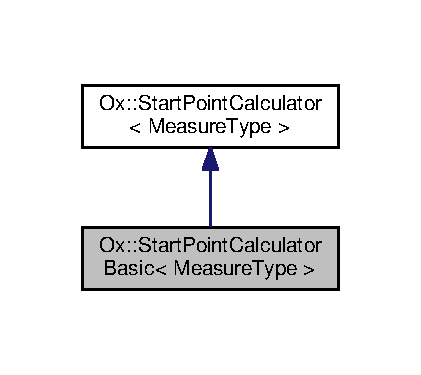
\includegraphics[width=202pt]{class_ox_1_1_start_point_calculator_basic__inherit__graph}
\end{center}
\end{figure}


Collaboration diagram for Ox\-:\-:Start\-Point\-Calculator\-Basic$<$ Measure\-Type $>$\-:
\nopagebreak
\begin{figure}[H]
\begin{center}
\leavevmode
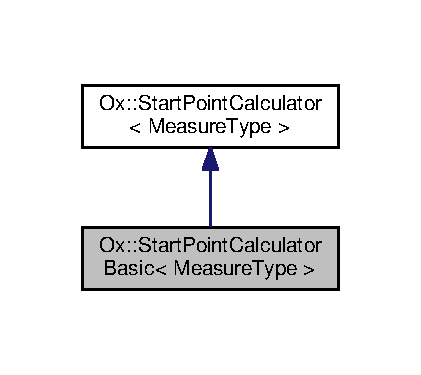
\includegraphics[width=202pt]{class_ox_1_1_start_point_calculator_basic__coll__graph}
\end{center}
\end{figure}
\subsection*{Public Member Functions}
\begin{DoxyCompactItemize}
\item 
virtual int \hyperlink{class_ox_1_1_start_point_calculator_basic_a9d227adf887f091f180f3e2fd37ab2cc}{calculate\-Start\-Point} ()
\item 
virtual \hyperlink{class_ox_1_1_start_point_calculator}{Start\-Point\-Calculator}\\*
$<$ Measure\-Type $>$ $\ast$ \hyperlink{class_ox_1_1_start_point_calculator_basic_a65bb3460d9358f3d9538648e221c8247}{new\-By\-Cloning} ()
\item 
\hypertarget{class_ox_1_1_start_point_calculator_basic_a7e55561e008088c26459c210e95b69e1}{virtual \hyperlink{class_ox_1_1_start_point_calculator_basic_a7e55561e008088c26459c210e95b69e1}{$\sim$\-Start\-Point\-Calculator\-Basic} ()}\label{class_ox_1_1_start_point_calculator_basic_a7e55561e008088c26459c210e95b69e1}

\begin{DoxyCompactList}\small\item\em do not forget about the virtual destructor, see \href{https://stackoverflow.com/questions/461203/when-to-use-virtual-destructors}{\tt https\-://stackoverflow.\-com/questions/461203/when-\/to-\/use-\/virtual-\/destructors} \end{DoxyCompactList}\end{DoxyCompactItemize}
\subsection*{Additional Inherited Members}


\subsection{Detailed Description}
\subsubsection*{template$<$typename Measure\-Type$>$class Ox\-::\-Start\-Point\-Calculator\-Basic$<$ Measure\-Type $>$}


\begin{DoxyTemplParams}{Template Parameters}
{\em Measure\-Type} & \\
\hline
\end{DoxyTemplParams}


\subsection{Member Function Documentation}
\hypertarget{class_ox_1_1_start_point_calculator_basic_a9d227adf887f091f180f3e2fd37ab2cc}{\index{Ox\-::\-Start\-Point\-Calculator\-Basic@{Ox\-::\-Start\-Point\-Calculator\-Basic}!calculate\-Start\-Point@{calculate\-Start\-Point}}
\index{calculate\-Start\-Point@{calculate\-Start\-Point}!Ox::StartPointCalculatorBasic@{Ox\-::\-Start\-Point\-Calculator\-Basic}}
\subsubsection[{calculate\-Start\-Point}]{\setlength{\rightskip}{0pt plus 5cm}template$<$typename Measure\-Type$>$ virtual int {\bf Ox\-::\-Start\-Point\-Calculator\-Basic}$<$ Measure\-Type $>$\-::calculate\-Start\-Point (
\begin{DoxyParamCaption}
{}
\end{DoxyParamCaption}
)\hspace{0.3cm}{\ttfamily [inline]}, {\ttfamily [virtual]}}}\label{class_ox_1_1_start_point_calculator_basic_a9d227adf887f091f180f3e2fd37ab2cc}
the most important function of this class \begin{DoxyReturn}{Returns}
success/failure 
\end{DoxyReturn}


Implements \hyperlink{class_ox_1_1_start_point_calculator_a9d1132410d68eb16f3f71ec4015c0b2f}{Ox\-::\-Start\-Point\-Calculator$<$ Measure\-Type $>$}.

\hypertarget{class_ox_1_1_start_point_calculator_basic_a65bb3460d9358f3d9538648e221c8247}{\index{Ox\-::\-Start\-Point\-Calculator\-Basic@{Ox\-::\-Start\-Point\-Calculator\-Basic}!new\-By\-Cloning@{new\-By\-Cloning}}
\index{new\-By\-Cloning@{new\-By\-Cloning}!Ox::StartPointCalculatorBasic@{Ox\-::\-Start\-Point\-Calculator\-Basic}}
\subsubsection[{new\-By\-Cloning}]{\setlength{\rightskip}{0pt plus 5cm}template$<$typename Measure\-Type$>$ virtual {\bf Start\-Point\-Calculator}$<$Measure\-Type$>$$\ast$ {\bf Ox\-::\-Start\-Point\-Calculator\-Basic}$<$ Measure\-Type $>$\-::new\-By\-Cloning (
\begin{DoxyParamCaption}
{}
\end{DoxyParamCaption}
)\hspace{0.3cm}{\ttfamily [inline]}, {\ttfamily [virtual]}}}\label{class_ox_1_1_start_point_calculator_basic_a65bb3460d9358f3d9538648e221c8247}
cloning \begin{DoxyReturn}{Returns}

\end{DoxyReturn}


Implements \hyperlink{class_ox_1_1_start_point_calculator_acd2a221872002157f232e1e7f73a1859}{Ox\-::\-Start\-Point\-Calculator$<$ Measure\-Type $>$}.



The documentation for this class was generated from the following file\-:\begin{DoxyCompactItemize}
\item 
lib/\hyperlink{_ox_start_point_calculator_basic_8h}{Ox\-Start\-Point\-Calculator\-Basic.\-h}\end{DoxyCompactItemize}

\hypertarget{class_ox_1_1_start_point_calculator_shmolli}{}\section{Ox\+:\+:Start\+Point\+Calculator\+Shmolli$<$ Measure\+Type $>$ Class Template Reference}
\label{class_ox_1_1_start_point_calculator_shmolli}\index{Ox\+::\+Start\+Point\+Calculator\+Shmolli$<$ Measure\+Type $>$@{Ox\+::\+Start\+Point\+Calculator\+Shmolli$<$ Measure\+Type $>$}}


{\ttfamily \#include $<$Ox\+Start\+Point\+Calculator\+Shmolli.\+h$>$}



Inheritance diagram for Ox\+:\+:Start\+Point\+Calculator\+Shmolli$<$ Measure\+Type $>$\+:
\nopagebreak
\begin{figure}[H]
\begin{center}
\leavevmode
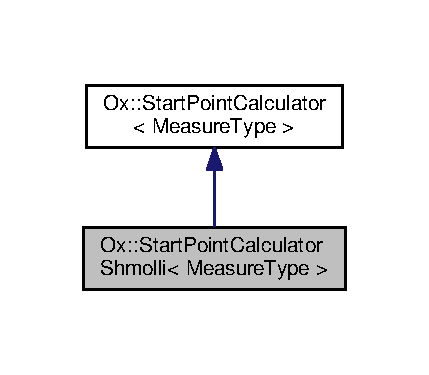
\includegraphics[width=206pt]{class_ox_1_1_start_point_calculator_shmolli__inherit__graph}
\end{center}
\end{figure}


Collaboration diagram for Ox\+:\+:Start\+Point\+Calculator\+Shmolli$<$ Measure\+Type $>$\+:
\nopagebreak
\begin{figure}[H]
\begin{center}
\leavevmode
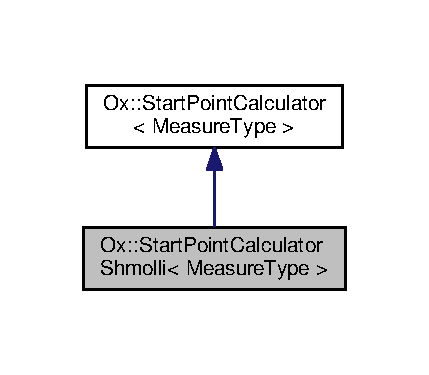
\includegraphics[width=206pt]{class_ox_1_1_start_point_calculator_shmolli__coll__graph}
\end{center}
\end{figure}
\subsection*{Public Member Functions}
\begin{DoxyCompactItemize}
\item 
virtual int \hyperlink{class_ox_1_1_start_point_calculator_shmolli_acd0913906ed0d4301b78b5329cc3d62f}{calculate\+Start\+Point} ()
\item 
int {\bfseries set\+Start\+Point\+To\+Default} ()\hypertarget{class_ox_1_1_start_point_calculator_shmolli_ac4e1b932329096fd43f77c4ddf2bd804}{}\label{class_ox_1_1_start_point_calculator_shmolli_ac4e1b932329096fd43f77c4ddf2bd804}

\item 
int {\bfseries calculate\+Start\+Point\+S\+KP} (int n\+Samples, const Measure\+Type $\ast$inv\+Times, const Measure\+Type $\ast$ysignal\+Input, const double $\ast$signs, Measure\+Type $\ast$init\+Point)\hypertarget{class_ox_1_1_start_point_calculator_shmolli_aaf776712e300b190928e793eec54cc47}{}\label{class_ox_1_1_start_point_calculator_shmolli_aaf776712e300b190928e793eec54cc47}

\item 
\hyperlink{class_ox_1_1_start_point_calculator_shmolli_afc823088ce6d5d0ac3e1eec161ede9e2}{Start\+Point\+Calculator\+Shmolli} ()\hypertarget{class_ox_1_1_start_point_calculator_shmolli_afc823088ce6d5d0ac3e1eec161ede9e2}{}\label{class_ox_1_1_start_point_calculator_shmolli_afc823088ce6d5d0ac3e1eec161ede9e2}

\begin{DoxyCompactList}\small\item\em constructor \end{DoxyCompactList}\item 
\hyperlink{class_ox_1_1_start_point_calculator_shmolli_a65b9fc02c5e9483e9b3b39ee0962e201}{Start\+Point\+Calculator\+Shmolli} (const \hyperlink{class_ox_1_1_start_point_calculator_shmolli}{Start\+Point\+Calculator\+Shmolli} \&old)\hypertarget{class_ox_1_1_start_point_calculator_shmolli_a65b9fc02c5e9483e9b3b39ee0962e201}{}\label{class_ox_1_1_start_point_calculator_shmolli_a65b9fc02c5e9483e9b3b39ee0962e201}

\begin{DoxyCompactList}\small\item\em copy constructor \end{DoxyCompactList}\item 
virtual \hyperlink{class_ox_1_1_start_point_calculator}{Start\+Point\+Calculator}$<$ Measure\+Type $>$ $\ast$ \hyperlink{class_ox_1_1_start_point_calculator_shmolli_ab3f7f6efa7fb6ac4ce1a93fb7ec42f85}{new\+By\+Cloning} ()
\item 
virtual \hyperlink{class_ox_1_1_start_point_calculator_shmolli_aaede509b017e5da6102a230ad979539a}{$\sim$\+Start\+Point\+Calculator\+Shmolli} ()\hypertarget{class_ox_1_1_start_point_calculator_shmolli_aaede509b017e5da6102a230ad979539a}{}\label{class_ox_1_1_start_point_calculator_shmolli_aaede509b017e5da6102a230ad979539a}

\begin{DoxyCompactList}\small\item\em do not forget about the virtual destructor, see \href{https://stackoverflow.com/questions/461203/when-to-use-virtual-destructors}{\tt https\+://stackoverflow.\+com/questions/461203/when-\/to-\/use-\/virtual-\/destructors} \end{DoxyCompactList}\end{DoxyCompactItemize}
\subsection*{Protected Attributes}
\begin{DoxyCompactItemize}
\item 
Measure\+Type {\bfseries \+\_\+\+Default\+Start\+Point} \mbox{[}3\mbox{]}\hypertarget{class_ox_1_1_start_point_calculator_shmolli_acb458533b900c9088d1dd7be30183ba0}{}\label{class_ox_1_1_start_point_calculator_shmolli_acb458533b900c9088d1dd7be30183ba0}

\end{DoxyCompactItemize}


\subsection{Detailed Description}
\subsubsection*{template$<$typename Measure\+Type$>$\\*
class Ox\+::\+Start\+Point\+Calculator\+Shmolli$<$ Measure\+Type $>$}


\begin{DoxyTemplParams}{Template Parameters}
{\em Measure\+Type} & \\
\hline
\end{DoxyTemplParams}


\subsection{Member Function Documentation}
\index{Ox\+::\+Start\+Point\+Calculator\+Shmolli@{Ox\+::\+Start\+Point\+Calculator\+Shmolli}!calculate\+Start\+Point@{calculate\+Start\+Point}}
\index{calculate\+Start\+Point@{calculate\+Start\+Point}!Ox\+::\+Start\+Point\+Calculator\+Shmolli@{Ox\+::\+Start\+Point\+Calculator\+Shmolli}}
\subsubsection[{\texorpdfstring{calculate\+Start\+Point()}{calculateStartPoint()}}]{\setlength{\rightskip}{0pt plus 5cm}template$<$typename Measure\+Type$>$ virtual int {\bf Ox\+::\+Start\+Point\+Calculator\+Shmolli}$<$ Measure\+Type $>$\+::calculate\+Start\+Point (
\begin{DoxyParamCaption}
{}
\end{DoxyParamCaption}
)\hspace{0.3cm}{\ttfamily [inline]}, {\ttfamily [virtual]}}\hypertarget{class_ox_1_1_start_point_calculator_shmolli_acd0913906ed0d4301b78b5329cc3d62f}{}\label{class_ox_1_1_start_point_calculator_shmolli_acd0913906ed0d4301b78b5329cc3d62f}
the most important function of this class \begin{DoxyReturn}{Returns}
same as calculate\+Start\+Point\+S\+KP 
\end{DoxyReturn}


Implements \hyperlink{class_ox_1_1_start_point_calculator_a9d1132410d68eb16f3f71ec4015c0b2f}{Ox\+::\+Start\+Point\+Calculator$<$ Measure\+Type $>$}.

\index{Ox\+::\+Start\+Point\+Calculator\+Shmolli@{Ox\+::\+Start\+Point\+Calculator\+Shmolli}!new\+By\+Cloning@{new\+By\+Cloning}}
\index{new\+By\+Cloning@{new\+By\+Cloning}!Ox\+::\+Start\+Point\+Calculator\+Shmolli@{Ox\+::\+Start\+Point\+Calculator\+Shmolli}}
\subsubsection[{\texorpdfstring{new\+By\+Cloning()}{newByCloning()}}]{\setlength{\rightskip}{0pt plus 5cm}template$<$typename Measure\+Type$>$ virtual {\bf Start\+Point\+Calculator}$<$Measure\+Type$>$$\ast$ {\bf Ox\+::\+Start\+Point\+Calculator\+Shmolli}$<$ Measure\+Type $>$\+::new\+By\+Cloning (
\begin{DoxyParamCaption}
{}
\end{DoxyParamCaption}
)\hspace{0.3cm}{\ttfamily [inline]}, {\ttfamily [virtual]}}\hypertarget{class_ox_1_1_start_point_calculator_shmolli_ab3f7f6efa7fb6ac4ce1a93fb7ec42f85}{}\label{class_ox_1_1_start_point_calculator_shmolli_ab3f7f6efa7fb6ac4ce1a93fb7ec42f85}
cloning \begin{DoxyReturn}{Returns}

\end{DoxyReturn}


Implements \hyperlink{class_ox_1_1_start_point_calculator_acd2a221872002157f232e1e7f73a1859}{Ox\+::\+Start\+Point\+Calculator$<$ Measure\+Type $>$}.



The documentation for this class was generated from the following file\+:\begin{DoxyCompactItemize}
\item 
lib/\hyperlink{_ox_start_point_calculator_shmolli_8h}{Ox\+Start\+Point\+Calculator\+Shmolli.\+h}\end{DoxyCompactItemize}

\hypertarget{class_ox_1_1_test_data}{\section{Ox\-:\-:Test\-Data$<$ Measure\-Type $>$ Class Template Reference}
\label{class_ox_1_1_test_data}\index{Ox\-::\-Test\-Data$<$ Measure\-Type $>$@{Ox\-::\-Test\-Data$<$ Measure\-Type $>$}}
}
\subsection*{Public Member Functions}
\begin{DoxyCompactItemize}
\item 
\hypertarget{class_ox_1_1_test_data_add19d13b8ec2404fc5d6ebf4ee79a231}{{\bfseries Test\-Data} (char $\ast$file\-Path)}\label{class_ox_1_1_test_data_add19d13b8ec2404fc5d6ebf4ee79a231}

\item 
\hypertarget{class_ox_1_1_test_data_a4e75699c035937ff96fa131505870208}{virtual std\-::vector$<$ Measure\-Type $>$ {\bfseries get\-Signal\-Mag} () const }\label{class_ox_1_1_test_data_a4e75699c035937ff96fa131505870208}

\item 
\hypertarget{class_ox_1_1_test_data_a287f28ddb03f9acc694528441b57c375}{virtual std\-::vector$<$ Measure\-Type $>$ {\bfseries get\-Signal\-Pha} () const }\label{class_ox_1_1_test_data_a287f28ddb03f9acc694528441b57c375}

\item 
\hypertarget{class_ox_1_1_test_data_a414b631b105104920740e51dcc4a3948}{virtual std\-::vector$<$ Measure\-Type $>$ {\bfseries get\-Signs} () const }\label{class_ox_1_1_test_data_a414b631b105104920740e51dcc4a3948}

\item 
\hypertarget{class_ox_1_1_test_data_a0dafaca55a2c3d57ff2106b518b3fada}{virtual std\-::vector$<$ Measure\-Type $>$ {\bfseries get\-Signal} () const }\label{class_ox_1_1_test_data_a0dafaca55a2c3d57ff2106b518b3fada}

\item 
\hypertarget{class_ox_1_1_test_data_acec1269baa03bfa45845f94f3bc15abe}{virtual std\-::vector$<$ Measure\-Type $>$ {\bfseries get\-Inv\-Times} () const }\label{class_ox_1_1_test_data_acec1269baa03bfa45845f94f3bc15abe}

\item 
\hypertarget{class_ox_1_1_test_data_a68a2cefeed3da1c1dac7a34256b9d640}{virtual std\-::vector$<$ Measure\-Type $>$ {\bfseries get\-Results\-Molli} () const }\label{class_ox_1_1_test_data_a68a2cefeed3da1c1dac7a34256b9d640}

\item 
\hypertarget{class_ox_1_1_test_data_aece21264e7f357c50e2d157f077127f5}{virtual std\-::vector$<$ Measure\-Type $>$ {\bfseries get\-Results\-Shmolli} () const }\label{class_ox_1_1_test_data_aece21264e7f357c50e2d157f077127f5}

\item 
\hypertarget{class_ox_1_1_test_data_a9f625acf214f62d6cdfee00c924ef9b0}{virtual const Measure\-Type $\ast$ {\bfseries get\-Signal\-Mag\-Ptr} () const }\label{class_ox_1_1_test_data_a9f625acf214f62d6cdfee00c924ef9b0}

\item 
\hypertarget{class_ox_1_1_test_data_aafe59c86537fb24e513443e34f2b506d}{virtual const Measure\-Type $\ast$ {\bfseries get\-Signal\-Pha\-Ptr} () const }\label{class_ox_1_1_test_data_aafe59c86537fb24e513443e34f2b506d}

\item 
\hypertarget{class_ox_1_1_test_data_a98127c877fabc49a7112489e928cda05}{virtual const Measure\-Type $\ast$ {\bfseries get\-Signs\-Ptr} () const }\label{class_ox_1_1_test_data_a98127c877fabc49a7112489e928cda05}

\item 
\hypertarget{class_ox_1_1_test_data_a7c52dbd7292dfafd5e9d95eb9d701e19}{virtual const Measure\-Type $\ast$ {\bfseries get\-Signal\-Ptr} () const }\label{class_ox_1_1_test_data_a7c52dbd7292dfafd5e9d95eb9d701e19}

\item 
\hypertarget{class_ox_1_1_test_data_ad6f19708661e0722df977b8dacbf88e7}{virtual const Measure\-Type $\ast$ {\bfseries get\-Inv\-Times\-Ptr} () const }\label{class_ox_1_1_test_data_ad6f19708661e0722df977b8dacbf88e7}

\item 
\hypertarget{class_ox_1_1_test_data_a1cb0dc25db322b7ba075e0ab7f5d6567}{virtual const Measure\-Type $\ast$ {\bfseries get\-Results\-Molli\-Ptr} () const }\label{class_ox_1_1_test_data_a1cb0dc25db322b7ba075e0ab7f5d6567}

\item 
\hypertarget{class_ox_1_1_test_data_ad822f6946548df6c68cf6cb007030702}{virtual const Measure\-Type $\ast$ {\bfseries get\-Results\-Shmolli\-Ptr} () const }\label{class_ox_1_1_test_data_ad822f6946548df6c68cf6cb007030702}

\item 
\hypertarget{class_ox_1_1_test_data_a93fc01cb722f3cadbaa530068c0079da}{virtual int {\bfseries get\-N\-Samples} () const }\label{class_ox_1_1_test_data_a93fc01cb722f3cadbaa530068c0079da}

\item 
\hypertarget{class_ox_1_1_test_data_a4c5bb0b0296218d61c608a8592900c39}{void {\bfseries copy\-Str\-Vector\-To\-Member\-Vector} (std\-::vector$<$ std\-::string $>$ str\-Vector, std\-::vector$<$ Measure\-Type $>$ \&member\-Vector)}\label{class_ox_1_1_test_data_a4c5bb0b0296218d61c608a8592900c39}

\item 
\hypertarget{class_ox_1_1_test_data_ac19364ea614dad392eefb4dbeb8a7903}{void {\bfseries disp} ()}\label{class_ox_1_1_test_data_ac19364ea614dad392eefb4dbeb8a7903}

\item 
\hypertarget{class_ox_1_1_test_data_a3de0e44dba2bd5e3b7556d662575378a}{{\footnotesize template$<$typename T\-Y\-P\-E $>$ }\\void {\bfseries print\-Vector} (std\-::vector$<$ T\-Y\-P\-E $>$ my\-Vector, std\-::string my\-Vector\-Name)}\label{class_ox_1_1_test_data_a3de0e44dba2bd5e3b7556d662575378a}

\end{DoxyCompactItemize}
\subsection*{Protected Member Functions}
\begin{DoxyCompactItemize}
\item 
\hypertarget{class_ox_1_1_test_data_a014e56191a98df90450c0b6fa2abc45d}{void {\bfseries calc\-Signal} ()}\label{class_ox_1_1_test_data_a014e56191a98df90450c0b6fa2abc45d}

\end{DoxyCompactItemize}
\subsection*{Protected Attributes}
\begin{DoxyCompactItemize}
\item 
\hypertarget{class_ox_1_1_test_data_a41f65fef5fa534f713cb8a229e5ae14d}{int {\bfseries \-\_\-n\-Samples}}\label{class_ox_1_1_test_data_a41f65fef5fa534f713cb8a229e5ae14d}

\item 
\hypertarget{class_ox_1_1_test_data_a180e0158dc204212fd4879690b2ea3ad}{std\-::vector$<$ Measure\-Type $>$ {\bfseries \-\_\-signal\-Mag}}\label{class_ox_1_1_test_data_a180e0158dc204212fd4879690b2ea3ad}

\item 
\hypertarget{class_ox_1_1_test_data_a5012bab7b7943d05b33151aae38efcc1}{std\-::vector$<$ Measure\-Type $>$ {\bfseries \-\_\-signal\-Pha}}\label{class_ox_1_1_test_data_a5012bab7b7943d05b33151aae38efcc1}

\item 
\hypertarget{class_ox_1_1_test_data_a3d844b169fbdbfcb77d5ef0bf527f554}{std\-::vector$<$ Measure\-Type $>$ {\bfseries \-\_\-signal}}\label{class_ox_1_1_test_data_a3d844b169fbdbfcb77d5ef0bf527f554}

\item 
\hypertarget{class_ox_1_1_test_data_a9e22c4f291064b0c49f7c8007e77b40a}{std\-::vector$<$ Measure\-Type $>$ {\bfseries \-\_\-signs}}\label{class_ox_1_1_test_data_a9e22c4f291064b0c49f7c8007e77b40a}

\item 
\hypertarget{class_ox_1_1_test_data_a4a72325aa7d38c4cac1762a47b7eed1a}{std\-::vector$<$ Measure\-Type $>$ {\bfseries \-\_\-inv\-Times}}\label{class_ox_1_1_test_data_a4a72325aa7d38c4cac1762a47b7eed1a}

\item 
\hypertarget{class_ox_1_1_test_data_a91ae0ccd1b9dea3b83bfc4d7c300dbb0}{std\-::vector$<$ Measure\-Type $>$ {\bfseries \-\_\-results\-Molli}}\label{class_ox_1_1_test_data_a91ae0ccd1b9dea3b83bfc4d7c300dbb0}

\item 
\hypertarget{class_ox_1_1_test_data_ac549cebd93bd96747a68e3680442adfd}{std\-::vector$<$ Measure\-Type $>$ {\bfseries \-\_\-results\-Shmolli}}\label{class_ox_1_1_test_data_ac549cebd93bd96747a68e3680442adfd}

\end{DoxyCompactItemize}


The documentation for this class was generated from the following files\-:\begin{DoxyCompactItemize}
\item 
tests/\hyperlink{_ox_test_data_8h}{Ox\-Test\-Data.\-h}\item 
tests/\hyperlink{_ox_test_data_8hxx}{Ox\-Test\-Data.\-hxx}\end{DoxyCompactItemize}

\hypertarget{class_ox_1_1_test_image}{\section{Ox\-:\-:Test\-Image$<$ Measure\-Type $>$ Class Template Reference}
\label{class_ox_1_1_test_image}\index{Ox\-::\-Test\-Image$<$ Measure\-Type $>$@{Ox\-::\-Test\-Image$<$ Measure\-Type $>$}}
}
\subsection*{Public Member Functions}
\begin{DoxyCompactItemize}
\item 
\hypertarget{class_ox_1_1_test_image_a3b5ceff06d34b2ebd4a4ff215e156088}{{\bfseries Test\-Image} (int n\-Cols, int n\-Rows, std\-::vector$<$ std\-::string $>$ files\-Paths, std\-::vector$<$ int $>$ inv\-Times\-Order)}\label{class_ox_1_1_test_image_a3b5ceff06d34b2ebd4a4ff215e156088}

\item 
\hypertarget{class_ox_1_1_test_image_a794b321a180a2b19d88efc316e0d47aa}{{\bfseries Test\-Image} (int n\-Cols, int n\-Rows, std\-::vector$<$ std\-::string $>$ files\-Paths)}\label{class_ox_1_1_test_image_a794b321a180a2b19d88efc316e0d47aa}

\item 
\hypertarget{class_ox_1_1_test_image_aa802ece1484e88fd748b462c6e2a6cf9}{int {\bfseries init} (int n\-Cols, int n\-Rows, std\-::vector$<$ std\-::string $>$ files\-Paths, std\-::vector$<$ int $>$ inv\-Times\-Order)}\label{class_ox_1_1_test_image_aa802ece1484e88fd748b462c6e2a6cf9}

\item 
\hypertarget{class_ox_1_1_test_image_a6dda2e0b1c2f9d285a29007a14441be3}{virtual Measure\-Type $\ast$ {\bfseries get\-Inv\-Times\-Ptr} ()}\label{class_ox_1_1_test_image_a6dda2e0b1c2f9d285a29007a14441be3}

\item 
\hypertarget{class_ox_1_1_test_image_accd975ba34db53a323810f506e0953d1}{virtual std\-::vector$<$ Measure\-Type $>$ {\bfseries get\-Inv\-Times} () const }\label{class_ox_1_1_test_image_accd975ba34db53a323810f506e0953d1}

\item 
\hypertarget{class_ox_1_1_test_image_a825435d601877f1595b5b04d8f2df2c1}{virtual Measure\-Type $\ast$ {\bfseries get\-Image\-Mag\-Ptr} () const }\label{class_ox_1_1_test_image_a825435d601877f1595b5b04d8f2df2c1}

\item 
\hypertarget{class_ox_1_1_test_image_a6e7c4c1195dfd0c1938c913b230b48a7}{virtual Measure\-Type $\ast$ {\bfseries get\-Image\-Pha\-Ptr} () const }\label{class_ox_1_1_test_image_a6e7c4c1195dfd0c1938c913b230b48a7}

\item 
\hypertarget{class_ox_1_1_test_image_a9da80782972a99cae274cde3de03bbda}{virtual Measure\-Type $\ast$ {\bfseries get\-Image\-Results\-Molli\-Ptr} () const }\label{class_ox_1_1_test_image_a9da80782972a99cae274cde3de03bbda}

\item 
\hypertarget{class_ox_1_1_test_image_aef09efd3eb4b1a37d3b6b479d1e4a016}{virtual Measure\-Type $\ast$ {\bfseries get\-Image\-Results\-Shmolli\-Ptr} () const }\label{class_ox_1_1_test_image_aef09efd3eb4b1a37d3b6b479d1e4a016}

\item 
\hypertarget{class_ox_1_1_test_image_af5a9aadf12db9fdff87ed6aff4e0a2ef}{virtual int {\bfseries get\-N\-Cols} () const }\label{class_ox_1_1_test_image_af5a9aadf12db9fdff87ed6aff4e0a2ef}

\item 
\hypertarget{class_ox_1_1_test_image_acdc29d077640af69c4caac7c60d31cd6}{virtual int {\bfseries get\-N\-Rows} () const }\label{class_ox_1_1_test_image_acdc29d077640af69c4caac7c60d31cd6}

\item 
\hypertarget{class_ox_1_1_test_image_a87559c865b1f365c0bd7cfc9c5939d2b}{virtual int {\bfseries get\-N\-Samples} () const }\label{class_ox_1_1_test_image_a87559c865b1f365c0bd7cfc9c5939d2b}

\end{DoxyCompactItemize}
\subsection*{Protected Attributes}
\begin{DoxyCompactItemize}
\item 
\hypertarget{class_ox_1_1_test_image_aede6d17394f5b1d7aee6287c17482bed}{int {\bfseries \-\_\-n\-Cols}}\label{class_ox_1_1_test_image_aede6d17394f5b1d7aee6287c17482bed}

\item 
\hypertarget{class_ox_1_1_test_image_a2fca989633ec429545fefe579641eeb3}{int {\bfseries \-\_\-n\-Rows}}\label{class_ox_1_1_test_image_a2fca989633ec429545fefe579641eeb3}

\item 
\hypertarget{class_ox_1_1_test_image_a0b2de27b3ba5865c071a754c34e86bc7}{int {\bfseries \-\_\-n\-Samples}}\label{class_ox_1_1_test_image_a0b2de27b3ba5865c071a754c34e86bc7}

\item 
\hypertarget{class_ox_1_1_test_image_a9a3283dccb1476d113836134c3479328}{std\-::vector$<$ Measure\-Type $>$ {\bfseries \-\_\-inv\-Times}}\label{class_ox_1_1_test_image_a9a3283dccb1476d113836134c3479328}

\item 
\hypertarget{class_ox_1_1_test_image_aa7d94bb56b584ccae5619fcf5e55218c}{std\-::vector$<$ int $>$ {\bfseries \-\_\-inv\-Times\-Order}}\label{class_ox_1_1_test_image_aa7d94bb56b584ccae5619fcf5e55218c}

\item 
\hypertarget{class_ox_1_1_test_image_aa6d8862446566b0f1bc313de05cedd28}{Measure\-Type $\ast$ {\bfseries \-\_\-image\-Mag}}\label{class_ox_1_1_test_image_aa6d8862446566b0f1bc313de05cedd28}

\item 
\hypertarget{class_ox_1_1_test_image_a108ccefc1c986d4ad3265ec5601841c5}{Measure\-Type $\ast$ {\bfseries \-\_\-image\-Pha}}\label{class_ox_1_1_test_image_a108ccefc1c986d4ad3265ec5601841c5}

\item 
\hypertarget{class_ox_1_1_test_image_aa942d21740af38bc720db46a77fcea6c}{Measure\-Type $\ast$ {\bfseries \-\_\-image\-Results\-Molli}}\label{class_ox_1_1_test_image_aa942d21740af38bc720db46a77fcea6c}

\item 
\hypertarget{class_ox_1_1_test_image_abab3b898dade1792c251df511357be13}{Measure\-Type $\ast$ {\bfseries \-\_\-image\-Results\-Shmolli}}\label{class_ox_1_1_test_image_abab3b898dade1792c251df511357be13}

\end{DoxyCompactItemize}


The documentation for this class was generated from the following files\-:\begin{DoxyCompactItemize}
\item 
tests/\hyperlink{_ox_test_image_8h}{Ox\-Test\-Image.\-h}\item 
tests/\hyperlink{_ox_test_image_8hxx}{Ox\-Test\-Image.\-hxx}\end{DoxyCompactItemize}

\hypertarget{struct_ox_1_1_tomato_options}{\section{Ox\-:\-:Tomato\-Options$<$ T\-Y\-P\-E $>$ Struct Template Reference}
\label{struct_ox_1_1_tomato_options}\index{Ox\-::\-Tomato\-Options$<$ T\-Y\-P\-E $>$@{Ox\-::\-Tomato\-Options$<$ T\-Y\-P\-E $>$}}
}


{\ttfamily \#include $<$Ox\-Factory\-Of\-Fitters.\-h$>$}

\subsection*{Public Member Functions}
\begin{DoxyCompactItemize}
\item 
void \hyperlink{struct_ox_1_1_tomato_options_a76497b53cadad720af7ff0f83b99096b}{init} ()
\item 
\hyperlink{struct_ox_1_1_tomato_options_a974a7659d7eaefe712b1bb00cbd46a93}{Tomato\-Options} ()
\item 
\hyperlink{struct_ox_1_1_tomato_options_abd502ef8966b09c671e2b7a5b565ce38}{Tomato\-Options} (std\-::string file\-Path)
\item 
\hypertarget{struct_ox_1_1_tomato_options_a9630620338003eb675fdfe242449c915}{int {\bfseries find\-In\-Array} (int size, const char $\ast$name\-Array\mbox{[}$\,$\mbox{]}, std\-::string name)}\label{struct_ox_1_1_tomato_options_a9630620338003eb675fdfe242449c915}

\item 
\hypertarget{struct_ox_1_1_tomato_options_ab50a9d1d7044fa64878b9b7141fd4c81}{void {\bfseries print\-Current} ()}\label{struct_ox_1_1_tomato_options_ab50a9d1d7044fa64878b9b7141fd4c81}

\item 
\hypertarget{struct_ox_1_1_tomato_options_a8c763b89efcc2122205363a7e743afa9}{int {\bfseries export\-To\-Yaml} ()}\label{struct_ox_1_1_tomato_options_a8c763b89efcc2122205363a7e743afa9}

\item 
\hypertarget{struct_ox_1_1_tomato_options_a858797a020bbb2504cfcf389bec9bca2}{int {\bfseries export\-To\-Yaml} (std\-::string file\-Path)}\label{struct_ox_1_1_tomato_options_a858797a020bbb2504cfcf389bec9bca2}

\end{DoxyCompactItemize}
\subsection*{Public Attributes}
\begin{DoxyCompactItemize}
\item 
\hypertarget{struct_ox_1_1_tomato_options_ad123055506ec1c4c73b397a5f771d2e7}{std\-::vector$<$ std\-::string $>$ {\bfseries files\-\_\-magnitude}}\label{struct_ox_1_1_tomato_options_ad123055506ec1c4c73b397a5f771d2e7}

\item 
\hypertarget{struct_ox_1_1_tomato_options_acd13f26343647d05164a33cb5b4163f3}{std\-::vector$<$ std\-::string $>$ {\bfseries files\-\_\-phase}}\label{struct_ox_1_1_tomato_options_acd13f26343647d05164a33cb5b4163f3}

\item 
\hypertarget{struct_ox_1_1_tomato_options_aeffcb3fc69397596ce852699a2f3b05d}{std\-::string {\bfseries dir\-\_\-magnitude}}\label{struct_ox_1_1_tomato_options_aeffcb3fc69397596ce852699a2f3b05d}

\item 
\hypertarget{struct_ox_1_1_tomato_options_a92cabcc150b94b5b4c3dbea6e8ecb846}{std\-::string {\bfseries dir\-\_\-phase}}\label{struct_ox_1_1_tomato_options_a92cabcc150b94b5b4c3dbea6e8ecb846}

\item 
\hypertarget{struct_ox_1_1_tomato_options_af31a50b6e23004912a1512812c823a29}{std\-::string {\bfseries dir\-\_\-output\-\_\-map}}\label{struct_ox_1_1_tomato_options_af31a50b6e23004912a1512812c823a29}

\item 
\hypertarget{struct_ox_1_1_tomato_options_ab8e2816968affd97a0ba0b13c44c4c02}{std\-::string {\bfseries dir\-\_\-output\-\_\-fitparams}}\label{struct_ox_1_1_tomato_options_ab8e2816968affd97a0ba0b13c44c4c02}

\item 
\hypertarget{struct_ox_1_1_tomato_options_a0d4ad4476a8817e68ead08d1b0645033}{calculators\-Type\-\_\-t {\bfseries parameter\-\_\-to\-\_\-map}}\label{struct_ox_1_1_tomato_options_a0d4ad4476a8817e68ead08d1b0645033}

\item 
\hypertarget{struct_ox_1_1_tomato_options_a2d1d2149185ef71968980cf8c6afcf14}{fitters\-Type\-\_\-t {\bfseries fitting\-\_\-method}}\label{struct_ox_1_1_tomato_options_a2d1d2149185ef71968980cf8c6afcf14}

\item 
\hypertarget{struct_ox_1_1_tomato_options_aced156934915e4bb658d9f8433f69ee2}{functions\-Type\-\_\-t {\bfseries functions\-\_\-type}}\label{struct_ox_1_1_tomato_options_aced156934915e4bb658d9f8433f69ee2}

\item 
\hypertarget{struct_ox_1_1_tomato_options_a2cf923d6d04fb8cb510db2623e93119d}{sign\-Calculators\-Type\-\_\-t {\bfseries sign\-\_\-calc\-\_\-method}}\label{struct_ox_1_1_tomato_options_a2cf923d6d04fb8cb510db2623e93119d}

\item 
\hypertarget{struct_ox_1_1_tomato_options_a9da2993961d10c848b0860284900c869}{start\-Point\-Calculators\-Type\-\_\-t {\bfseries start\-\_\-point\-\_\-calc\-\_\-method}}\label{struct_ox_1_1_tomato_options_a9da2993961d10c848b0860284900c869}

\item 
\hypertarget{struct_ox_1_1_tomato_options_ae2ac4c46e46b4d183c6944771701040b}{Measure\-Type {\bfseries f\-Tolerance}}\label{struct_ox_1_1_tomato_options_ae2ac4c46e46b4d183c6944771701040b}

\item 
\hypertarget{struct_ox_1_1_tomato_options_a9b864c01b6b0b4e4d5a56470f6c5f004}{int {\bfseries max\-\_\-function\-\_\-evals}}\label{struct_ox_1_1_tomato_options_a9b864c01b6b0b4e4d5a56470f6c5f004}

\item 
\hypertarget{struct_ox_1_1_tomato_options_a367c540e5413f8ffa3a6bc6ef5781b45}{bool {\bfseries use\-\_\-gradient}}\label{struct_ox_1_1_tomato_options_a367c540e5413f8ffa3a6bc6ef5781b45}

\item 
\hypertarget{struct_ox_1_1_tomato_options_af81d1a55409036109d253b313d59e972}{Measure\-Type {\bfseries mean\-\_\-cut\-\_\-off}}\label{struct_ox_1_1_tomato_options_af81d1a55409036109d253b313d59e972}

\item 
\hypertarget{struct_ox_1_1_tomato_options_ab245e10cf32b36c48d66208a5f505099}{Measure\-Type {\bfseries map\-\_\-scale\-\_\-factor}}\label{struct_ox_1_1_tomato_options_ab245e10cf32b36c48d66208a5f505099}

\item 
\hypertarget{struct_ox_1_1_tomato_options_aa762826a11ff767aa969bd66c29b577f}{bool {\bfseries use\-\_\-colorbar}}\label{struct_ox_1_1_tomato_options_aa762826a11ff767aa969bd66c29b577f}

\item 
\hypertarget{struct_ox_1_1_tomato_options_a54efb4945f2857ee4ed9e1d5552fc3dd}{int {\bfseries number\-\_\-of\-\_\-threads}}\label{struct_ox_1_1_tomato_options_a54efb4945f2857ee4ed9e1d5552fc3dd}

\item 
\hypertarget{struct_ox_1_1_tomato_options_a043a4cf0e29a4482406e95f27ab2f860}{bool {\bfseries visualise}}\label{struct_ox_1_1_tomato_options_a043a4cf0e29a4482406e95f27ab2f860}

\item 
\hypertarget{struct_ox_1_1_tomato_options_ab20a779c5a8dd371ec9356e3f9ce79c9}{int {\bfseries output\-\_\-map\-\_\-series\-\_\-number}}\label{struct_ox_1_1_tomato_options_ab20a779c5a8dd371ec9356e3f9ce79c9}

\item 
\hypertarget{struct_ox_1_1_tomato_options_a58664e816cde6eff746bd5abe4fe2d1c}{int {\bfseries output\-\_\-fitparams\-\_\-series\-\_\-number}}\label{struct_ox_1_1_tomato_options_a58664e816cde6eff746bd5abe4fe2d1c}

\item 
\hypertarget{struct_ox_1_1_tomato_options_a008c932c7d65248d2d82e0e654993384}{double {\bfseries calculation\-\_\-time}}\label{struct_ox_1_1_tomato_options_a008c932c7d65248d2d82e0e654993384}

\end{DoxyCompactItemize}


\subsection{Detailed Description}
\subsubsection*{template$<$typename T\-Y\-P\-E$>$struct Ox\-::\-Tomato\-Options$<$ T\-Y\-P\-E $>$}

Here you can configure different fitting methods 
\begin{DoxyTemplParams}{Template Parameters}
{\em T\-Y\-P\-E} & \\
\hline
\end{DoxyTemplParams}


\subsection{Constructor \& Destructor Documentation}
\hypertarget{struct_ox_1_1_tomato_options_a974a7659d7eaefe712b1bb00cbd46a93}{\index{Ox\-::\-Tomato\-Options@{Ox\-::\-Tomato\-Options}!Tomato\-Options@{Tomato\-Options}}
\index{Tomato\-Options@{Tomato\-Options}!Ox::TomatoOptions@{Ox\-::\-Tomato\-Options}}
\subsubsection[{Tomato\-Options}]{\setlength{\rightskip}{0pt plus 5cm}template$<$typename T\-Y\-P\-E$>$ {\bf Ox\-::\-Tomato\-Options}$<$ T\-Y\-P\-E $>$\-::{\bf Tomato\-Options} (
\begin{DoxyParamCaption}
{}
\end{DoxyParamCaption}
)\hspace{0.3cm}{\ttfamily [inline]}}}\label{struct_ox_1_1_tomato_options_a974a7659d7eaefe712b1bb00cbd46a93}
constructor with defaults \hypertarget{struct_ox_1_1_tomato_options_abd502ef8966b09c671e2b7a5b565ce38}{\index{Ox\-::\-Tomato\-Options@{Ox\-::\-Tomato\-Options}!Tomato\-Options@{Tomato\-Options}}
\index{Tomato\-Options@{Tomato\-Options}!Ox::TomatoOptions@{Ox\-::\-Tomato\-Options}}
\subsubsection[{Tomato\-Options}]{\setlength{\rightskip}{0pt plus 5cm}template$<$typename T\-Y\-P\-E$>$ {\bf Ox\-::\-Tomato\-Options}$<$ T\-Y\-P\-E $>$\-::{\bf Tomato\-Options} (
\begin{DoxyParamCaption}
\item[{std\-::string}]{file\-Path}
\end{DoxyParamCaption}
)\hspace{0.3cm}{\ttfamily [inline]}}}\label{struct_ox_1_1_tomato_options_abd502ef8966b09c671e2b7a5b565ce38}
constructor with parser 
\begin{DoxyParams}{Parameters}
{\em file\-Path} & \\
\hline
\end{DoxyParams}


\subsection{Member Function Documentation}
\hypertarget{struct_ox_1_1_tomato_options_a76497b53cadad720af7ff0f83b99096b}{\index{Ox\-::\-Tomato\-Options@{Ox\-::\-Tomato\-Options}!init@{init}}
\index{init@{init}!Ox::TomatoOptions@{Ox\-::\-Tomato\-Options}}
\subsubsection[{init}]{\setlength{\rightskip}{0pt plus 5cm}template$<$typename T\-Y\-P\-E$>$ void {\bf Ox\-::\-Tomato\-Options}$<$ T\-Y\-P\-E $>$\-::init (
\begin{DoxyParamCaption}
{}
\end{DoxyParamCaption}
)\hspace{0.3cm}{\ttfamily [inline]}}}\label{struct_ox_1_1_tomato_options_a76497b53cadad720af7ff0f83b99096b}
initialise the defaults done this way to work around delegating constructors in cpp98 

The documentation for this struct was generated from the following files\-:\begin{DoxyCompactItemize}
\item 
app/\hyperlink{_ox_factory_of_calculators_8h}{Ox\-Factory\-Of\-Calculators.\-h}\item 
app/\hyperlink{_tomato_options_8h}{Tomato\-Options.\-h}\end{DoxyCompactItemize}

\chapter{File Documentation}
\hypertarget{main_8cpp}{\section{app/main.cpp File Reference}
\label{main_8cpp}\index{app/main.\-cpp@{app/main.\-cpp}}
}


A Documented file with main.  


{\ttfamily \#include $<$iostream$>$}\\*
{\ttfamily \#include \char`\"{}yaml.\-h\char`\"{}}\\*
Include dependency graph for main.\-cpp\-:
\nopagebreak
\begin{figure}[H]
\begin{center}
\leavevmode
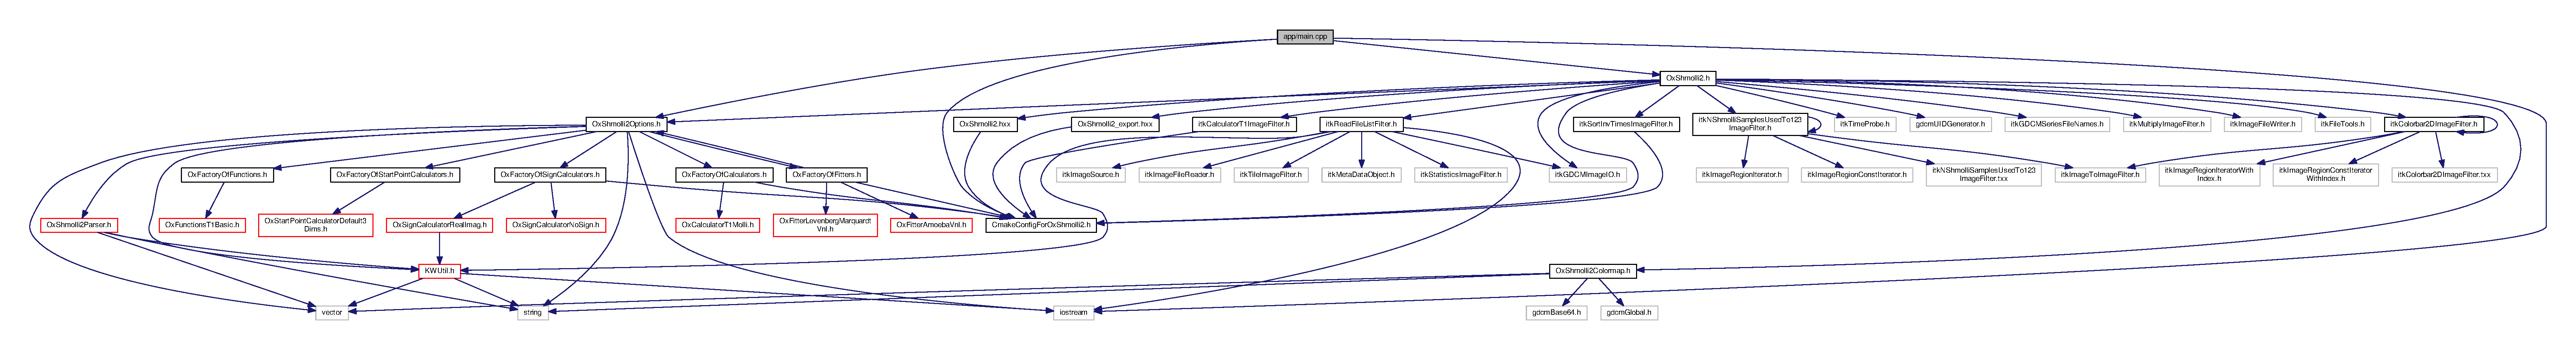
\includegraphics[width=198pt]{main_8cpp__incl}
\end{center}
\end{figure}
\subsection*{Functions}
\begin{DoxyCompactItemize}
\item 
int \hyperlink{main_8cpp_ae66f6b31b5ad750f1fe042a706a4e3d4}{main} ()
\end{DoxyCompactItemize}


\subsection{Detailed Description}
A Documented file with main. Details of the file should be here. \begin{DoxyAuthor}{Author}
Konrad Werys 
\end{DoxyAuthor}
\begin{DoxyDate}{Date}
2018/07/24 
\end{DoxyDate}


\subsection{Function Documentation}
\hypertarget{main_8cpp_ae66f6b31b5ad750f1fe042a706a4e3d4}{\index{main.\-cpp@{main.\-cpp}!main@{main}}
\index{main@{main}!main.cpp@{main.\-cpp}}
\subsubsection[{main}]{\setlength{\rightskip}{0pt plus 5cm}int main (
\begin{DoxyParamCaption}
{}
\end{DoxyParamCaption}
)}}\label{main_8cpp_ae66f6b31b5ad750f1fe042a706a4e3d4}
main \begin{DoxyReturn}{Returns}
always 0 
\end{DoxyReturn}

\hypertarget{_ox_factory_of_calculators_8h}{\section{app/\-Ox\-Factory\-Of\-Calculators.h File Reference}
\label{_ox_factory_of_calculators_8h}\index{app/\-Ox\-Factory\-Of\-Calculators.\-h@{app/\-Ox\-Factory\-Of\-Calculators.\-h}}
}
{\ttfamily \#include \char`\"{}Cmake\-Config\-For\-Tomato.\-h\char`\"{}}\\*
{\ttfamily \#include \char`\"{}Ox\-Calculator\-T1\-Molli.\-h\char`\"{}}\\*
{\ttfamily \#include \char`\"{}Ox\-Calculator\-T1\-Shmolli.\-h\char`\"{}}\\*
{\ttfamily \#include \char`\"{}Ox\-Calculator\-T2.\-h\char`\"{}}\\*
{\ttfamily \#include \char`\"{}Ox\-Calculator\-T2\-Truncation.\-h\char`\"{}}\\*
{\ttfamily \#include \char`\"{}Tomato\-Options.\-h\char`\"{}}\\*
Include dependency graph for Ox\-Factory\-Of\-Calculators.\-h\-:
\nopagebreak
\begin{figure}[H]
\begin{center}
\leavevmode
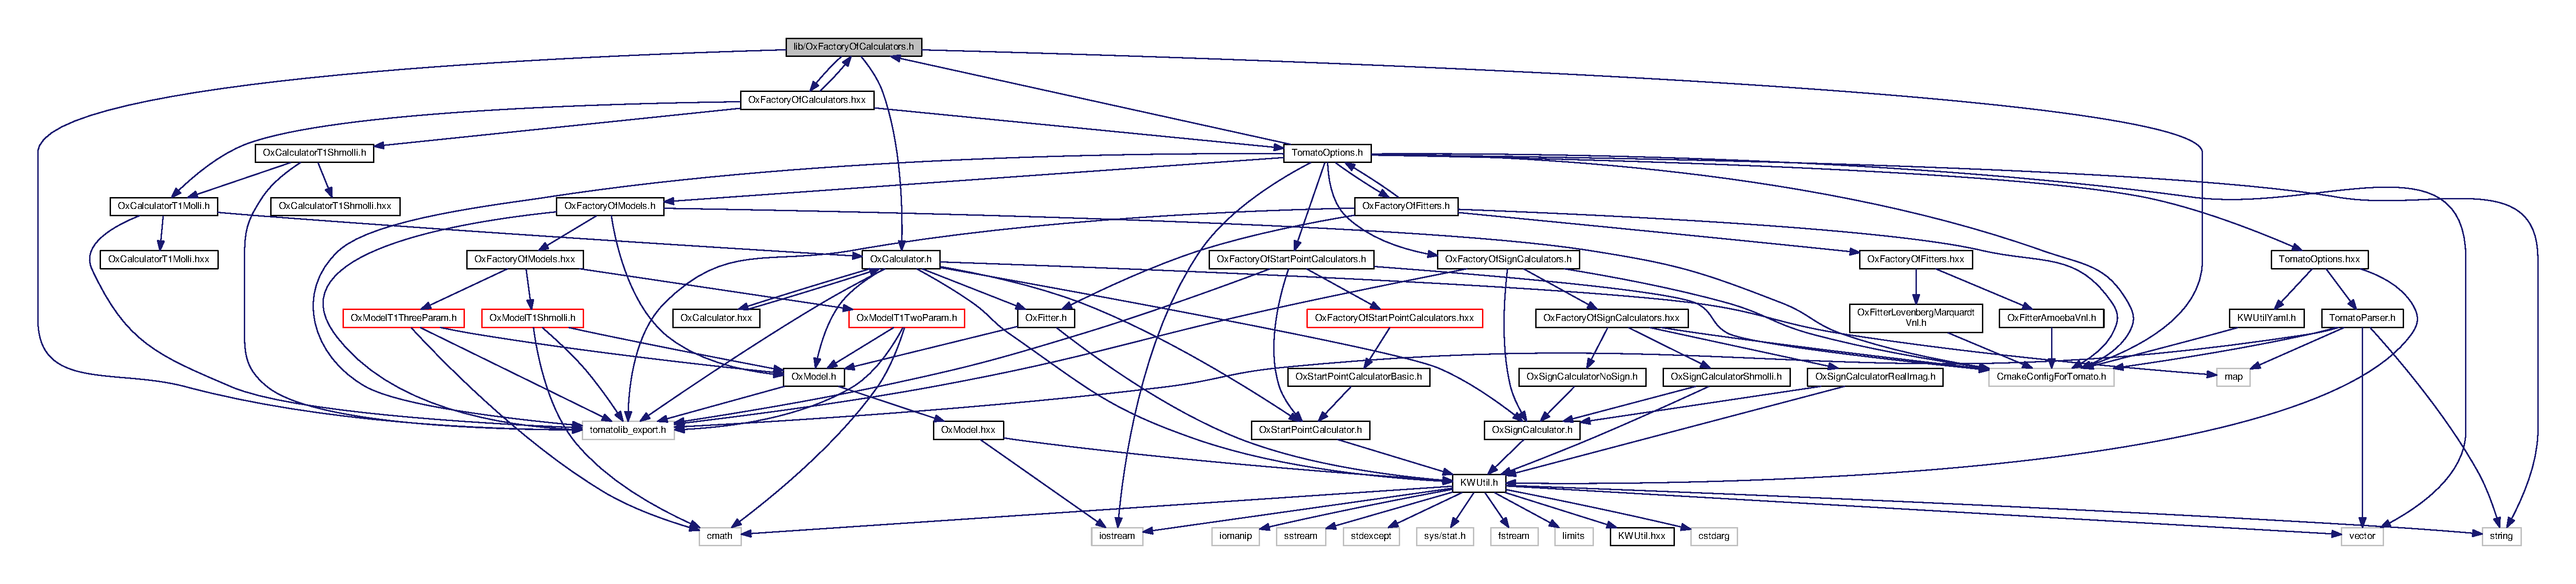
\includegraphics[width=350pt]{_ox_factory_of_calculators_8h__incl}
\end{center}
\end{figure}
This graph shows which files directly or indirectly include this file\-:
\nopagebreak
\begin{figure}[H]
\begin{center}
\leavevmode
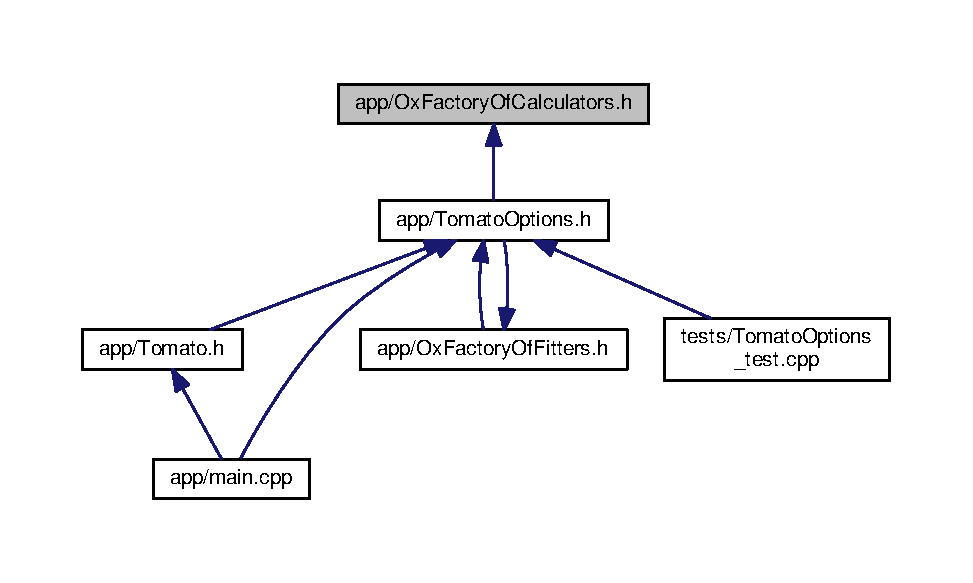
\includegraphics[width=311pt]{_ox_factory_of_calculators_8h__dep__incl}
\end{center}
\end{figure}
\subsection*{Classes}
\begin{DoxyCompactItemize}
\item 
struct \hyperlink{struct_ox_1_1_tomato_options}{Ox\-::\-Tomato\-Options$<$ T\-Y\-P\-E $>$}
\item 
class \hyperlink{class_ox_1_1_factory_of_calculators}{Ox\-::\-Factory\-Of\-Calculators$<$ T\-Y\-P\-E $>$}
\end{DoxyCompactItemize}
\subsection*{Enumerations}
\begin{DoxyCompactItemize}
\item 
enum {\bfseries param\-Type\-\_\-t} \{ {\bfseries T1} = 0, 
{\bfseries T2} = 1, 
{\bfseries T2star} = 2, 
{\bfseries Perf} = 3
 \}
\item 
enum {\bfseries calculators\-Type\-\_\-t} \{ \\*
{\bfseries T1\-\_\-\-M\-O\-L\-L\-I} = 0, 
{\bfseries T1\-\_\-\-S\-H\-M\-O\-L\-L\-I} = 1, 
{\bfseries T1\-\_\-\-S\-H\-M\-O\-L\-L\-I\-\_\-original} = 2, 
{\bfseries T2\-\_\-basic} = 3, 
\\*
{\bfseries T2\-\_\-truncation} = 4, 
{\bfseries last\-Calculator\-Type} = T2\-\_\-truncation
 \}
\end{DoxyCompactItemize}


\subsection{Detailed Description}
\begin{DoxyAuthor}{Author}
Konrad Werys 
\end{DoxyAuthor}
\begin{DoxyDate}{Date}
2018/08/18 
\end{DoxyDate}

\hypertarget{_ox_factory_of_fitters_8h}{\section{app/\-Ox\-Factory\-Of\-Fitters.h File Reference}
\label{_ox_factory_of_fitters_8h}\index{app/\-Ox\-Factory\-Of\-Fitters.\-h@{app/\-Ox\-Factory\-Of\-Fitters.\-h}}
}
{\ttfamily \#include \char`\"{}Cmake\-Config\-For\-Tomato.\-h\char`\"{}}\\*
{\ttfamily \#include \char`\"{}Tomato\-Options.\-h\char`\"{}}\\*
{\ttfamily \#include \char`\"{}Ox\-Fitter\-Amoeba\-Vnl.\-h\char`\"{}}\\*
{\ttfamily \#include \char`\"{}Ox\-Fitter\-Levenberg\-Marquardt\-Vnl.\-h\char`\"{}}\\*
Include dependency graph for Ox\-Factory\-Of\-Fitters.\-h\-:
\nopagebreak
\begin{figure}[H]
\begin{center}
\leavevmode
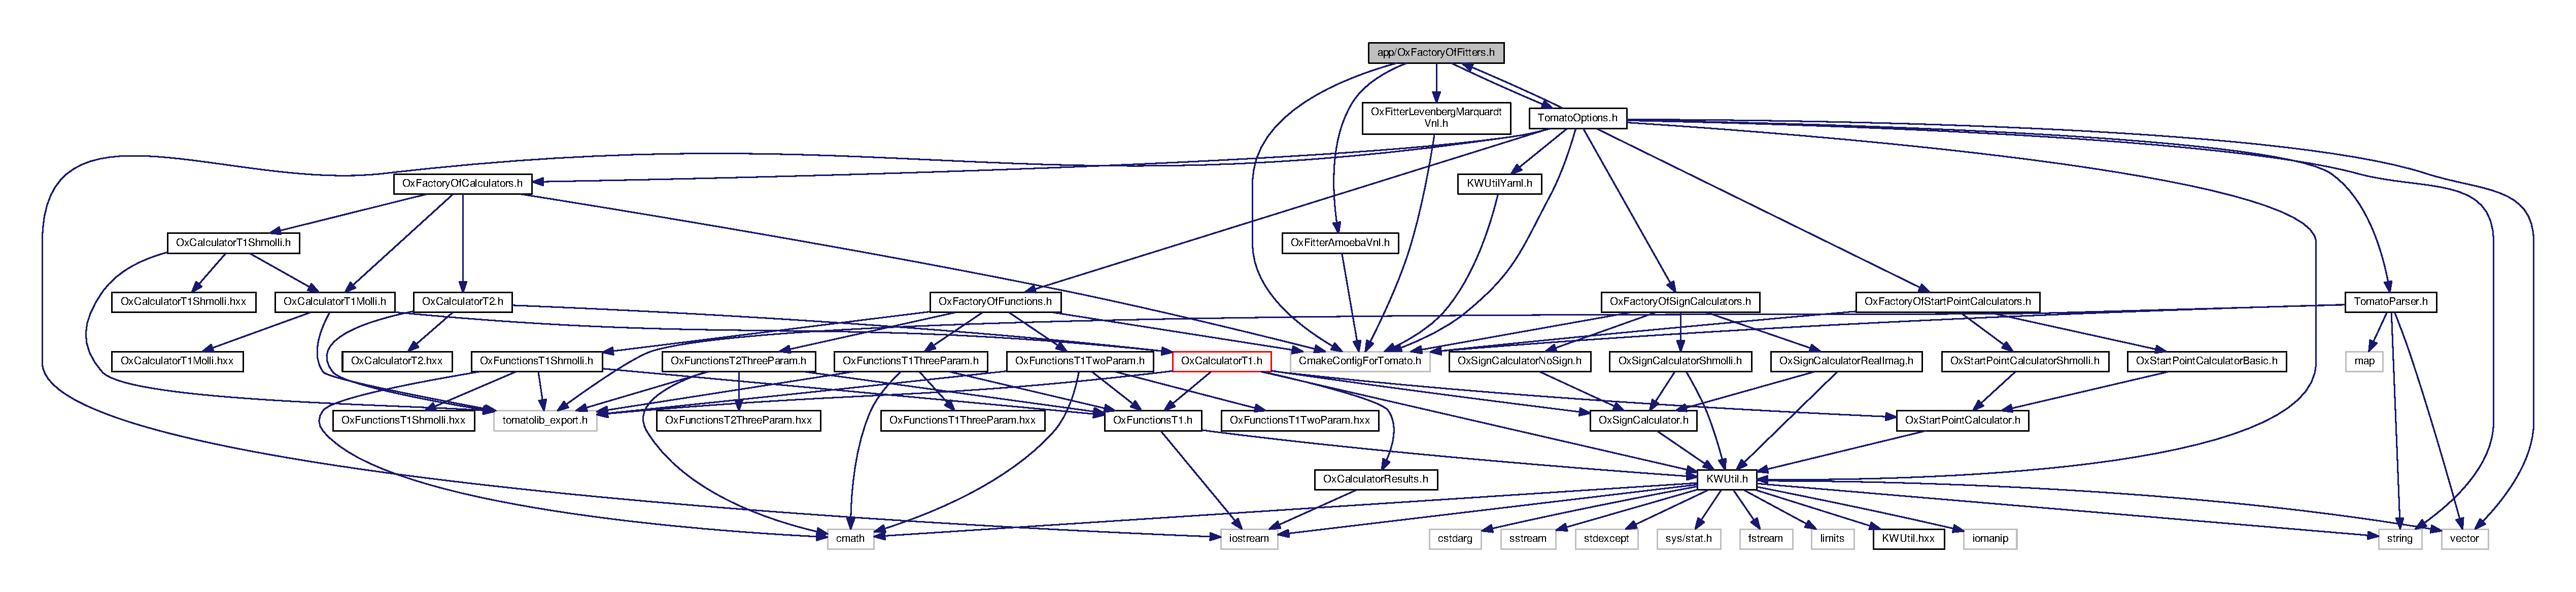
\includegraphics[width=350pt]{_ox_factory_of_fitters_8h__incl}
\end{center}
\end{figure}
This graph shows which files directly or indirectly include this file\-:
\nopagebreak
\begin{figure}[H]
\begin{center}
\leavevmode
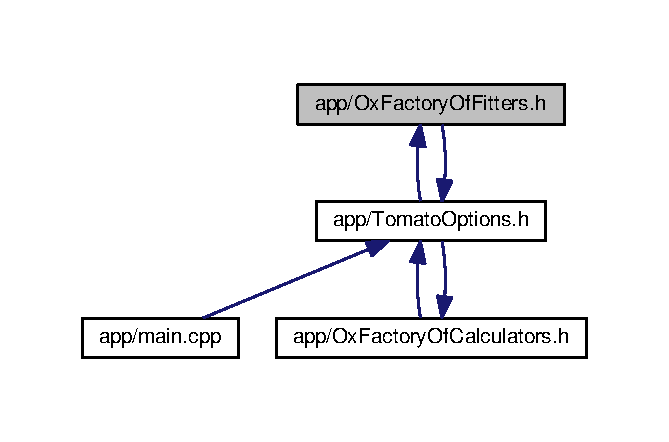
\includegraphics[width=215pt]{_ox_factory_of_fitters_8h__dep__incl}
\end{center}
\end{figure}
\subsection*{Classes}
\begin{DoxyCompactItemize}
\item 
struct \hyperlink{struct_ox_1_1_tomato_options}{Ox\-::\-Tomato\-Options$<$ T\-Y\-P\-E $>$}
\item 
class \hyperlink{class_ox_1_1_factory_of_fitters}{Ox\-::\-Factory\-Of\-Fitters$<$ T\-Y\-P\-E $>$}
\end{DoxyCompactItemize}
\subsection*{Enumerations}
\begin{DoxyCompactItemize}
\item 
enum {\bfseries fitters\-Type\-\_\-t} \{ {\bfseries Amoeba\-Vnl} = 0, 
{\bfseries Lev\-Mar\-Vnl} = 1, 
{\bfseries last\-Fitter\-Type} = Lev\-Mar\-Vnl
 \}
\end{DoxyCompactItemize}


\subsection{Detailed Description}
\begin{DoxyAuthor}{Author}
Konrad Werys 
\end{DoxyAuthor}
\begin{DoxyDate}{Date}
2018/08/18 
\end{DoxyDate}

\hypertarget{_ox_factory_of_sign_calculators_8h}{\section{app/\-Ox\-Factory\-Of\-Sign\-Calculators.h File Reference}
\label{_ox_factory_of_sign_calculators_8h}\index{app/\-Ox\-Factory\-Of\-Sign\-Calculators.\-h@{app/\-Ox\-Factory\-Of\-Sign\-Calculators.\-h}}
}
{\ttfamily \#include \char`\"{}Cmake\-Config\-For\-Tomato.\-h\char`\"{}}\\*
{\ttfamily \#include \char`\"{}Ox\-Sign\-Calculator\-No\-Sign.\-h\char`\"{}}\\*
{\ttfamily \#include \char`\"{}Ox\-Sign\-Calculator\-Real\-Imag.\-h\char`\"{}}\\*
Include dependency graph for Ox\-Factory\-Of\-Sign\-Calculators.\-h\-:
\nopagebreak
\begin{figure}[H]
\begin{center}
\leavevmode
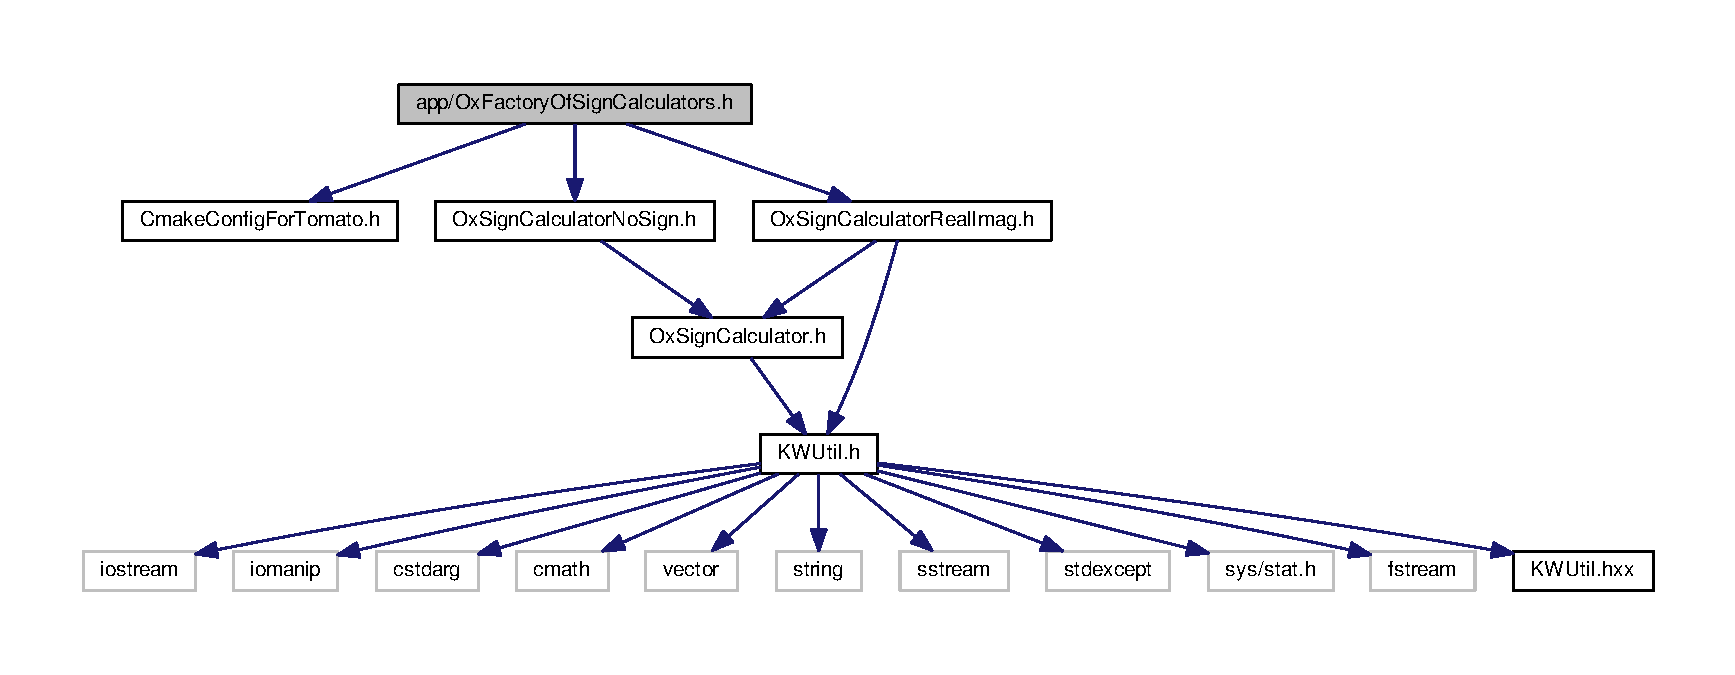
\includegraphics[width=350pt]{_ox_factory_of_sign_calculators_8h__incl}
\end{center}
\end{figure}
This graph shows which files directly or indirectly include this file\-:
\nopagebreak
\begin{figure}[H]
\begin{center}
\leavevmode
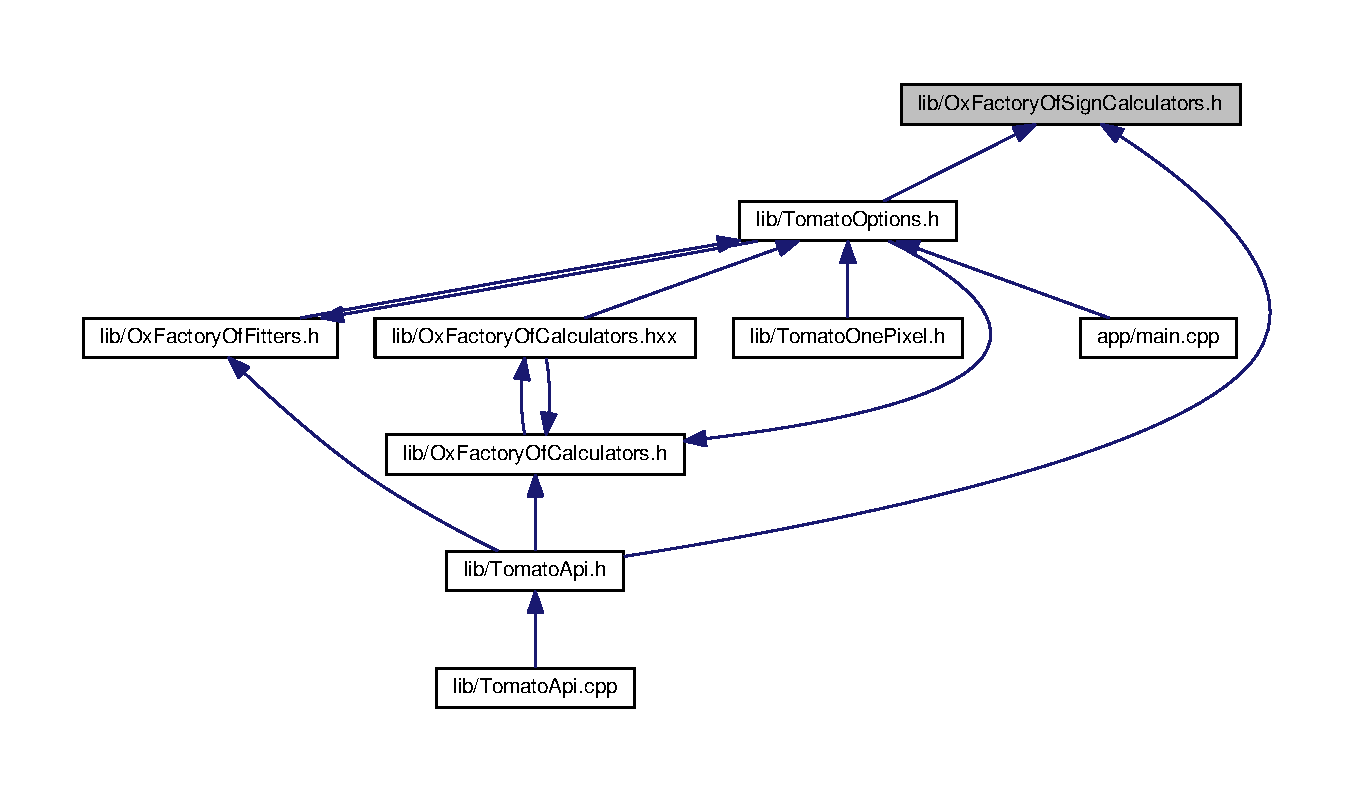
\includegraphics[width=321pt]{_ox_factory_of_sign_calculators_8h__dep__incl}
\end{center}
\end{figure}
\subsection*{Classes}
\begin{DoxyCompactItemize}
\item 
struct \hyperlink{struct_ox_1_1_tomato_options}{Ox\-::\-Tomato\-Options$<$ T\-Y\-P\-E $>$}
\item 
class \hyperlink{class_ox_1_1_factory_of_sign_calculators}{Ox\-::\-Factory\-Of\-Sign\-Calculators$<$ T\-Y\-P\-E $>$}
\end{DoxyCompactItemize}
\subsection*{Enumerations}
\begin{DoxyCompactItemize}
\item 
enum {\bfseries sign\-Calculators\-Type\-\_\-t} \{ {\bfseries No\-Sign} = 0, 
{\bfseries Real\-Imag} = 1, 
{\bfseries last\-Sign\-Calculator\-Type} = Real\-Imag
 \}
\end{DoxyCompactItemize}


\subsection{Detailed Description}
\begin{DoxyAuthor}{Author}
Konrad Werys 
\end{DoxyAuthor}
\begin{DoxyDate}{Date}
2018/08/18 
\end{DoxyDate}

\hypertarget{_ox_factory_of_start_point_calculators_8h}{}\section{lib/\+Ox\+Factory\+Of\+Start\+Point\+Calculators.h File Reference}
\label{_ox_factory_of_start_point_calculators_8h}\index{lib/\+Ox\+Factory\+Of\+Start\+Point\+Calculators.\+h@{lib/\+Ox\+Factory\+Of\+Start\+Point\+Calculators.\+h}}
{\ttfamily \#include \char`\"{}Cmake\+Config\+For\+Tomato.\+h\char`\"{}}\\*
{\ttfamily \#include \char`\"{}tomatolib\+\_\+export.\+h\char`\"{}}\\*
{\ttfamily \#include \char`\"{}Ox\+Start\+Point\+Calculator.\+h\char`\"{}}\\*
{\ttfamily \#include \char`\"{}Ox\+Factory\+Of\+Start\+Point\+Calculators.\+hxx\char`\"{}}\\*
Include dependency graph for Ox\+Factory\+Of\+Start\+Point\+Calculators.\+h\+:
\nopagebreak
\begin{figure}[H]
\begin{center}
\leavevmode
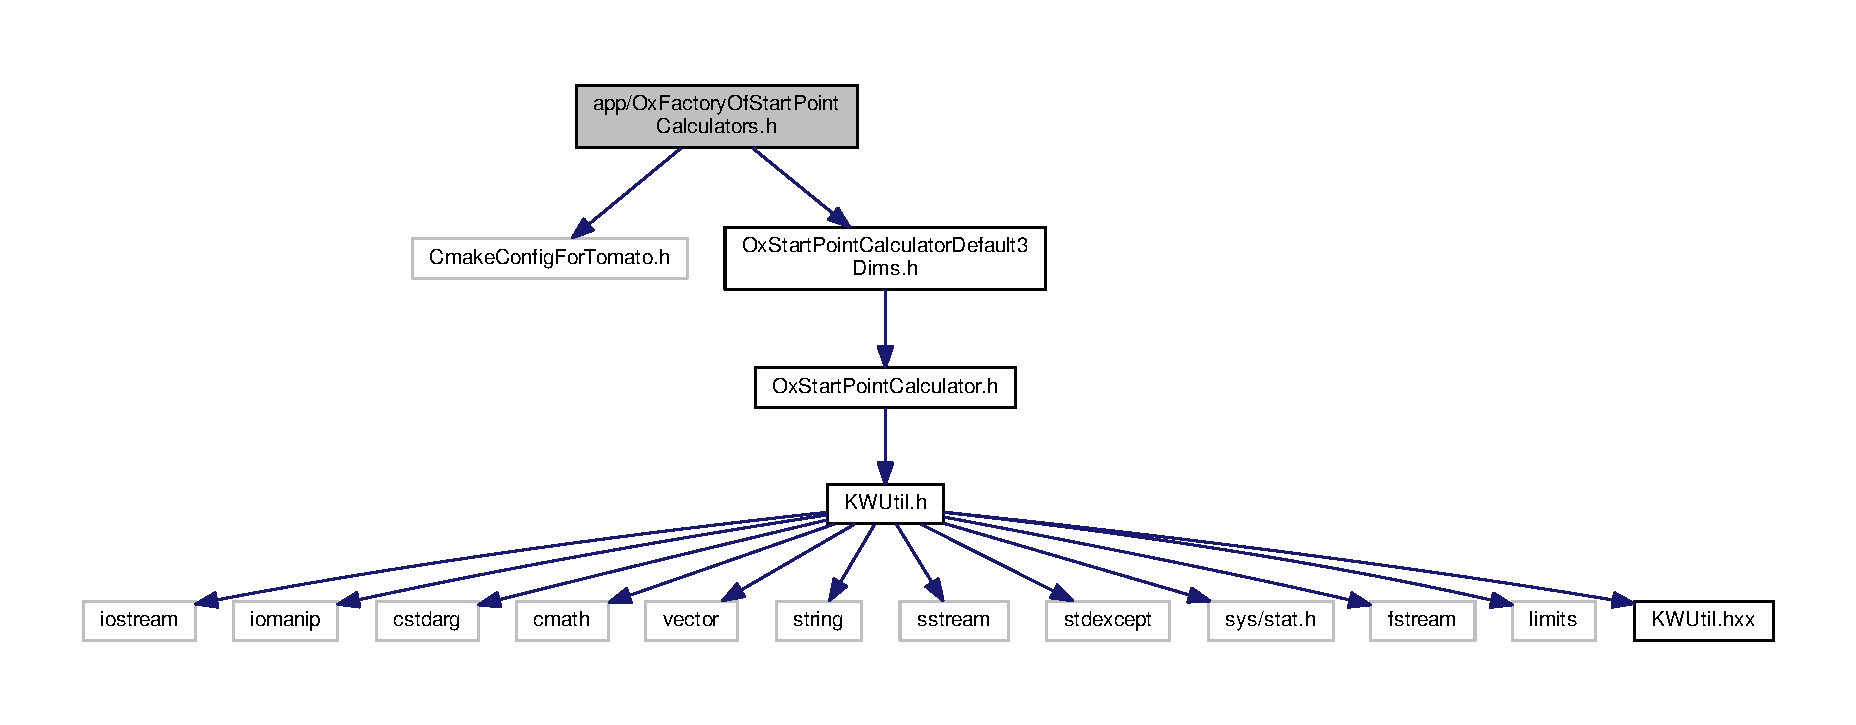
\includegraphics[width=350pt]{_ox_factory_of_start_point_calculators_8h__incl}
\end{center}
\end{figure}
This graph shows which files directly or indirectly include this file\+:
\nopagebreak
\begin{figure}[H]
\begin{center}
\leavevmode
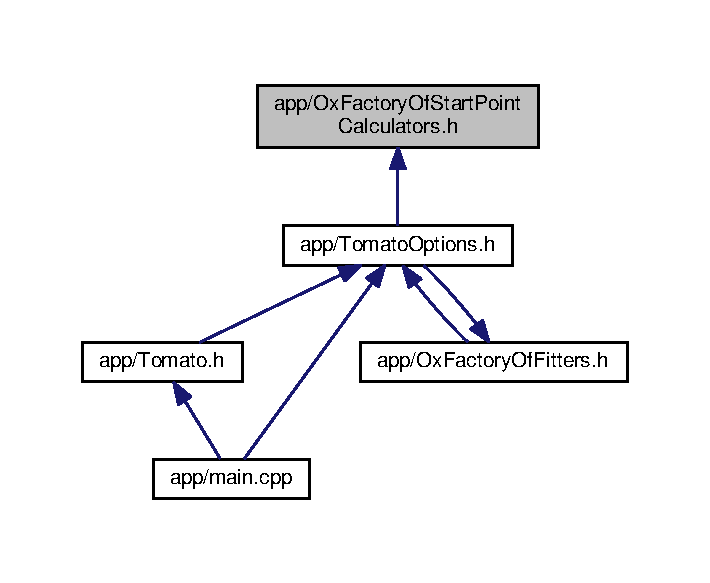
\includegraphics[width=350pt]{_ox_factory_of_start_point_calculators_8h__dep__incl}
\end{center}
\end{figure}
\subsection*{Classes}
\begin{DoxyCompactItemize}
\item 
class \hyperlink{class_ox_1_1_tomato_options}{Ox\+::\+Tomato\+Options$<$ Measure\+Type $>$}
\item 
class \hyperlink{class_ox_1_1_factory_of_start_point_calculators}{Ox\+::\+Factory\+Of\+Start\+Point\+Calculators$<$ T\+Y\+P\+E $>$}
\end{DoxyCompactItemize}
\subsection*{Enumerations}
\begin{DoxyCompactItemize}
\item 
enum {\bfseries start\+Point\+Calculators\+Type\+\_\+t} \{ {\bfseries Basic} = 0, 
{\bfseries Start\+Point\+S\+H\+M\+O\+L\+LI} = 1, 
{\bfseries No\+Start\+Point\+Calculators} = 2, 
{\bfseries last\+Start\+Point\+Calculator\+Type} = No\+Start\+Point\+Calculators
 \}\hypertarget{_ox_factory_of_start_point_calculators_8h_a50e0c7b888ecc4ab3505049584d879b1}{}\label{_ox_factory_of_start_point_calculators_8h_a50e0c7b888ecc4ab3505049584d879b1}

\end{DoxyCompactItemize}


\subsection{Detailed Description}
\begin{DoxyAuthor}{Author}
Konrad Werys 
\end{DoxyAuthor}
\begin{DoxyDate}{Date}
2018/08/18 
\end{DoxyDate}

\hypertarget{_ox_original_shmolli_dicom_reader_8h}{\section{app/\-Ox\-Original\-Shmolli\-Dicom\-Reader.h File Reference}
\label{_ox_original_shmolli_dicom_reader_8h}\index{app/\-Ox\-Original\-Shmolli\-Dicom\-Reader.\-h@{app/\-Ox\-Original\-Shmolli\-Dicom\-Reader.\-h}}
}
{\ttfamily \#include \char`\"{}Cmake\-Config\-For\-Tomato.\-h\char`\"{}}\\*
{\ttfamily \#include \char`\"{}tomatolib\-\_\-export.\-h\char`\"{}}\\*
Include dependency graph for Ox\-Original\-Shmolli\-Dicom\-Reader.\-h\-:
\nopagebreak
\begin{figure}[H]
\begin{center}
\leavevmode
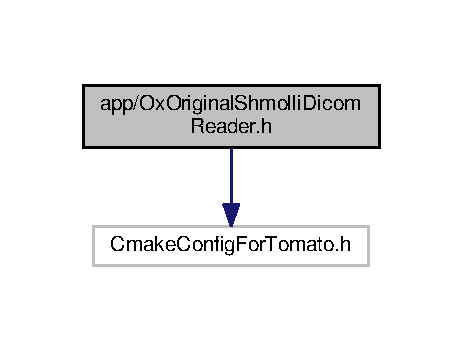
\includegraphics[width=327pt]{_ox_original_shmolli_dicom_reader_8h__incl}
\end{center}
\end{figure}
This graph shows which files directly or indirectly include this file\-:
\nopagebreak
\begin{figure}[H]
\begin{center}
\leavevmode
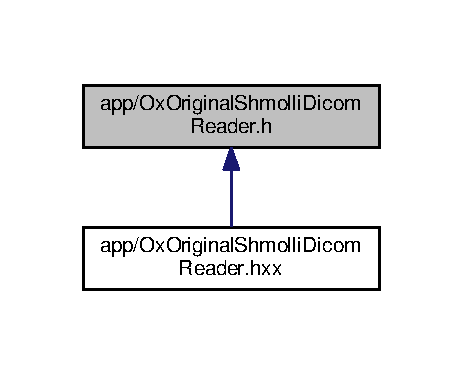
\includegraphics[width=222pt]{_ox_original_shmolli_dicom_reader_8h__dep__incl}
\end{center}
\end{figure}


\subsection{Detailed Description}
\begin{DoxyAuthor}{Author}
Konrad Werys 
\end{DoxyAuthor}
\begin{DoxyDate}{Date}
2018/08/24 
\end{DoxyDate}

\hypertarget{_ox_original_shmolli_dicom_reader_8hxx}{\section{app/\-Ox\-Original\-Shmolli\-Dicom\-Reader.hxx File Reference}
\label{_ox_original_shmolli_dicom_reader_8hxx}\index{app/\-Ox\-Original\-Shmolli\-Dicom\-Reader.\-hxx@{app/\-Ox\-Original\-Shmolli\-Dicom\-Reader.\-hxx}}
}
{\ttfamily \#include $<$itk\-Image\-File\-Reader\-K\-W.\-h$>$}\\*
{\ttfamily \#include \char`\"{}Ox\-Original\-Shmolli\-Dicom\-Reader.\-h\char`\"{}}\\*
Include dependency graph for Ox\-Original\-Shmolli\-Dicom\-Reader.\-hxx\-:
\nopagebreak
\begin{figure}[H]
\begin{center}
\leavevmode
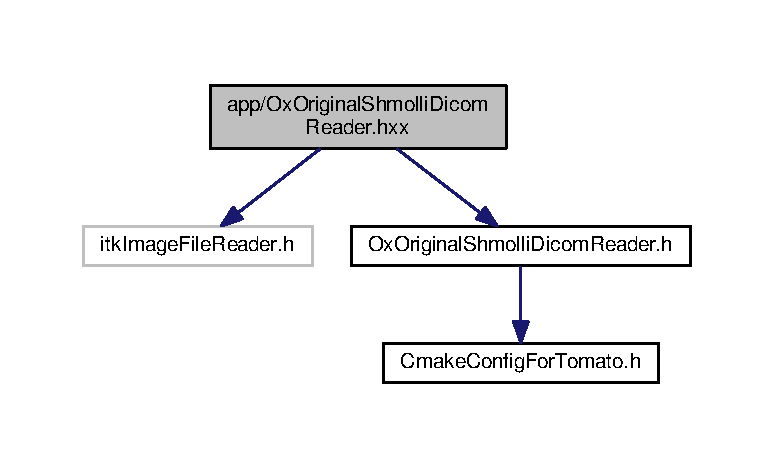
\includegraphics[width=350pt]{_ox_original_shmolli_dicom_reader_8hxx__incl}
\end{center}
\end{figure}


\subsection{Detailed Description}
\begin{DoxyAuthor}{Author}
Konrad Werys 
\end{DoxyAuthor}
\begin{DoxyDate}{Date}
2018/08/24 
\end{DoxyDate}

\hypertarget{_tomato_8h}{\section{app/\-Tomato.h File Reference}
\label{_tomato_8h}\index{app/\-Tomato.\-h@{app/\-Tomato.\-h}}
}
{\ttfamily \#include \char`\"{}Cmake\-Config\-For\-Tomato.\-h\char`\"{}}\\*
{\ttfamily \#include \char`\"{}Tomato\-Options.\-h\char`\"{}}\\*
{\ttfamily \#include \char`\"{}Tomato\-Colormap.\-h\char`\"{}}\\*
{\ttfamily \#include \char`\"{}itk\-Read\-File\-List\-Filter.\-h\char`\"{}}\\*
{\ttfamily \#include \char`\"{}itk\-Sort\-Inv\-Times\-Image\-Filter.\-h\char`\"{}}\\*
{\ttfamily \#include \char`\"{}itk\-Calculator\-T1\-Image\-Filter.\-h\char`\"{}}\\*
{\ttfamily \#include \char`\"{}itk\-Colorbar2\-D\-Image\-Filter.\-h\char`\"{}}\\*
{\ttfamily \#include \char`\"{}itk\-N\-Shmolli\-Samples\-Used\-To123\-Image\-Filter.\-h\char`\"{}}\\*
{\ttfamily \#include \char`\"{}itk\-Time\-Probe.\-h\char`\"{}}\\*
{\ttfamily \#include \char`\"{}gdcm\-U\-I\-D\-Generator.\-h\char`\"{}}\\*
{\ttfamily \#include \char`\"{}itk\-G\-D\-C\-M\-Image\-I\-O.\-h\char`\"{}}\\*
{\ttfamily \#include \char`\"{}itk\-G\-D\-C\-M\-Series\-File\-Names.\-h\char`\"{}}\\*
{\ttfamily \#include \char`\"{}itk\-Multiply\-Image\-Filter.\-h\char`\"{}}\\*
{\ttfamily \#include \char`\"{}itk\-Image\-File\-Writer.\-h\char`\"{}}\\*
{\ttfamily \#include \char`\"{}itk\-File\-Tools.\-h\char`\"{}}\\*
{\ttfamily \#include \char`\"{}itk\-Adapt\-Image\-Filter.\-h\char`\"{}}\\*
{\ttfamily \#include \char`\"{}Tomato.\-hxx\char`\"{}}\\*
{\ttfamily \#include \char`\"{}Tomato\-\_\-export.\-hxx\char`\"{}}\\*
Include dependency graph for Tomato.\-h\-:
\nopagebreak
\begin{figure}[H]
\begin{center}
\leavevmode
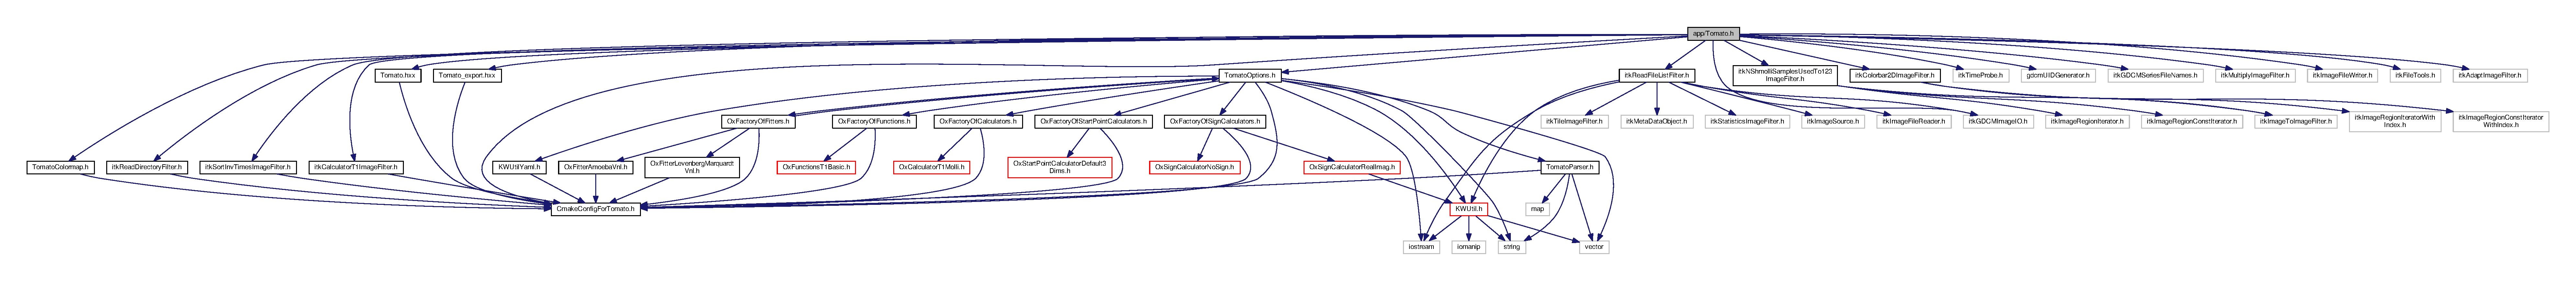
\includegraphics[width=350pt]{_tomato_8h__incl}
\end{center}
\end{figure}
This graph shows which files directly or indirectly include this file\-:
\nopagebreak
\begin{figure}[H]
\begin{center}
\leavevmode
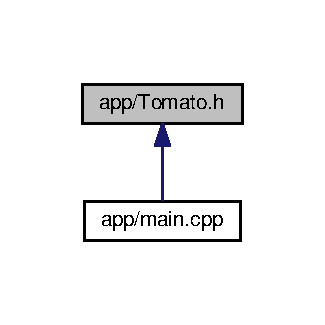
\includegraphics[width=321pt]{_tomato_8h__dep__incl}
\end{center}
\end{figure}


\subsection{Detailed Description}
\begin{DoxyAuthor}{Author}
Konrad Werys 
\end{DoxyAuthor}
\begin{DoxyDate}{Date}
2018/08/14 
\end{DoxyDate}

\hypertarget{_tomato_options_8h}{\section{app/\-Tomato\-Options.h File Reference}
\label{_tomato_options_8h}\index{app/\-Tomato\-Options.\-h@{app/\-Tomato\-Options.\-h}}
}
{\ttfamily \#include $<$iostream$>$}\\*
{\ttfamily \#include $<$vector$>$}\\*
{\ttfamily \#include $<$string$>$}\\*
{\ttfamily \#include \char`\"{}Cmake\-Config\-For\-Tomato.\-h\char`\"{}}\\*
{\ttfamily \#include \char`\"{}Ox\-Factory\-Of\-Calculators.\-h\char`\"{}}\\*
{\ttfamily \#include \char`\"{}Ox\-Factory\-Of\-Fitters.\-h\char`\"{}}\\*
{\ttfamily \#include \char`\"{}Ox\-Factory\-Of\-Functions.\-h\char`\"{}}\\*
{\ttfamily \#include \char`\"{}Ox\-Factory\-Of\-Sign\-Calculators.\-h\char`\"{}}\\*
{\ttfamily \#include \char`\"{}Ox\-Factory\-Of\-Start\-Point\-Calculators.\-h\char`\"{}}\\*
{\ttfamily \#include \char`\"{}Tomato\-Parser.\-h\char`\"{}}\\*
{\ttfamily \#include \char`\"{}K\-W\-Util.\-h\char`\"{}}\\*
{\ttfamily \#include \char`\"{}K\-W\-Util\-Yaml.\-h\char`\"{}}\\*
Include dependency graph for Tomato\-Options.\-h\-:
\nopagebreak
\begin{figure}[H]
\begin{center}
\leavevmode
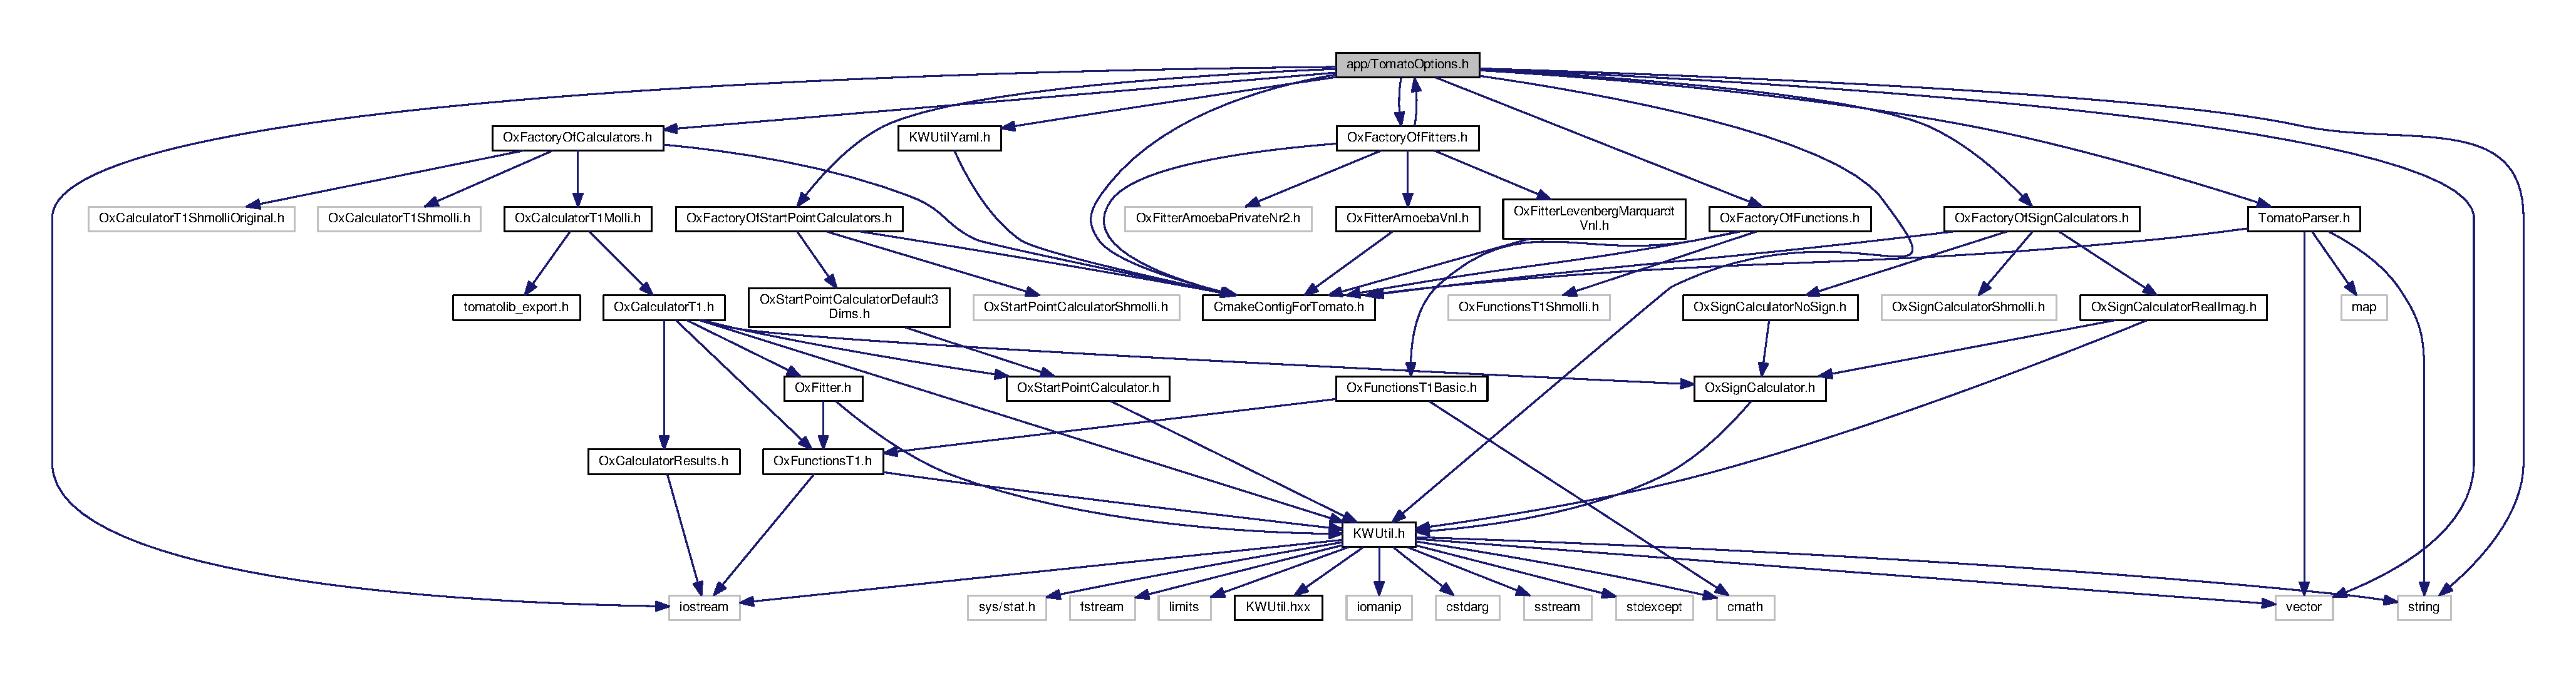
\includegraphics[width=350pt]{_tomato_options_8h__incl}
\end{center}
\end{figure}
This graph shows which files directly or indirectly include this file\-:
\nopagebreak
\begin{figure}[H]
\begin{center}
\leavevmode
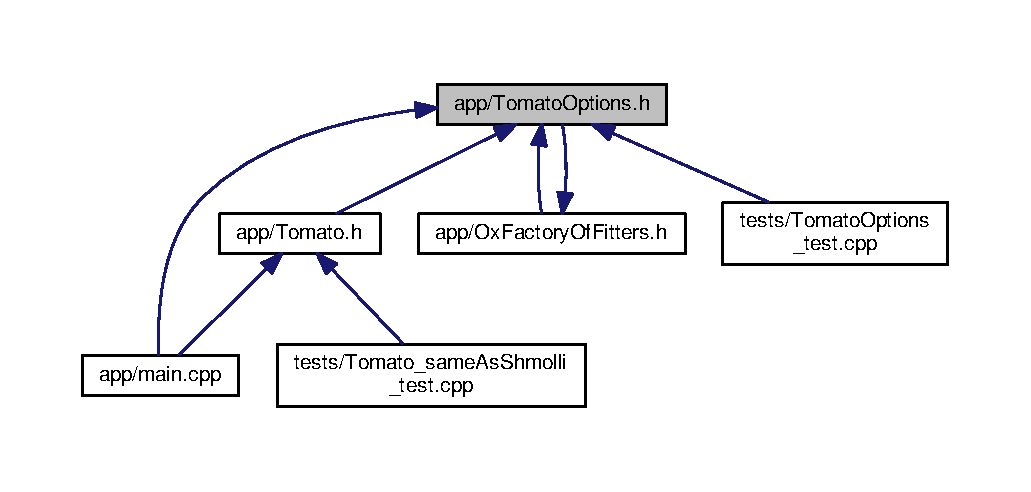
\includegraphics[width=301pt]{_tomato_options_8h__dep__incl}
\end{center}
\end{figure}
\subsection*{Classes}
\begin{DoxyCompactItemize}
\item 
struct \hyperlink{struct_ox_1_1_tomato_options}{Ox\-::\-Tomato\-Options$<$ T\-Y\-P\-E $>$}
\end{DoxyCompactItemize}
\subsection*{Macros}
\begin{DoxyCompactItemize}
\item 
\hypertarget{_tomato_options_8h_aa409ed425e3d493c4e1dcd695f6011df}{\#define {\bfseries Y\-A\-M\-L\-\_\-\-B\-U\-F\-F\-E\-R\-\_\-\-S\-I\-Z\-E}~65536}\label{_tomato_options_8h_aa409ed425e3d493c4e1dcd695f6011df}

\end{DoxyCompactItemize}


\subsection{Detailed Description}
\begin{DoxyAuthor}{Author}
Konrad Werys 
\end{DoxyAuthor}
\begin{DoxyDate}{Date}
2018/08/18 
\end{DoxyDate}

\hypertarget{itk_calculator_t1_image_filter_8h}{\section{lib/itk\-Calculator\-T1\-Image\-Filter.h File Reference}
\label{itk_calculator_t1_image_filter_8h}\index{lib/itk\-Calculator\-T1\-Image\-Filter.\-h@{lib/itk\-Calculator\-T1\-Image\-Filter.\-h}}
}
{\ttfamily \#include \char`\"{}Cmake\-Config\-For\-Ox\-Shmolli2.\-h\char`\"{}}\\*
Include dependency graph for itk\-Calculator\-T1\-Image\-Filter.\-h\-:
\nopagebreak
\begin{figure}[H]
\begin{center}
\leavevmode
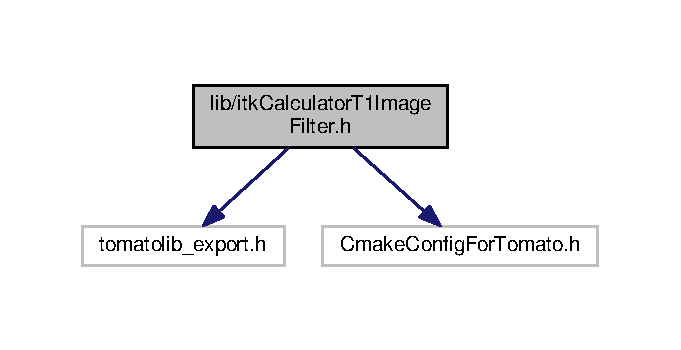
\includegraphics[width=228pt]{itk_calculator_t1_image_filter_8h__incl}
\end{center}
\end{figure}
This graph shows which files directly or indirectly include this file\-:
\nopagebreak
\begin{figure}[H]
\begin{center}
\leavevmode
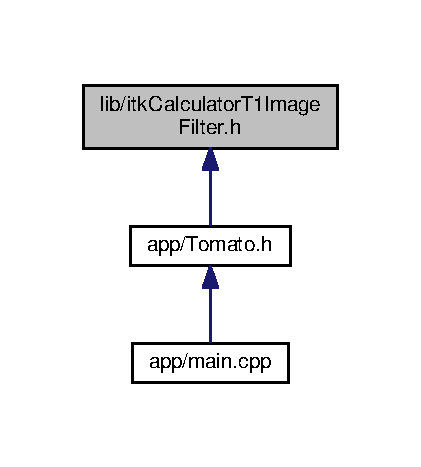
\includegraphics[width=202pt]{itk_calculator_t1_image_filter_8h__dep__incl}
\end{center}
\end{figure}


\subsection{Detailed Description}
\begin{DoxyAuthor}{Author}
Konrad Werys 
\end{DoxyAuthor}
\begin{DoxyDate}{Date}
2018/08/13 
\end{DoxyDate}

\hypertarget{itk_calculator_t1_image_filter_8hxx}{}\section{lib/itk\+Calculator\+T1\+Image\+Filter.hxx File Reference}
\label{itk_calculator_t1_image_filter_8hxx}\index{lib/itk\+Calculator\+T1\+Image\+Filter.\+hxx@{lib/itk\+Calculator\+T1\+Image\+Filter.\+hxx}}
{\ttfamily \#include \char`\"{}Cmake\+Config\+For\+Tomato.\+h\char`\"{}}\\*
Include dependency graph for itk\+Calculator\+T1\+Image\+Filter.\+hxx\+:
\nopagebreak
\begin{figure}[H]
\begin{center}
\leavevmode
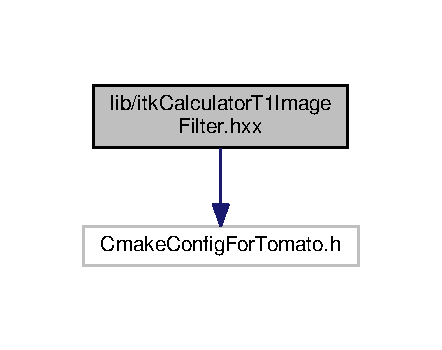
\includegraphics[width=212pt]{itk_calculator_t1_image_filter_8hxx__incl}
\end{center}
\end{figure}


\subsection{Detailed Description}
\begin{DoxyAuthor}{Author}
Konrad Werys 
\end{DoxyAuthor}
\begin{DoxyDate}{Date}
2018/08/13 
\end{DoxyDate}

\hypertarget{itk_calculator_t2_image_filter_8h}{\section{lib/itk\-Calculator\-T2\-Image\-Filter.h File Reference}
\label{itk_calculator_t2_image_filter_8h}\index{lib/itk\-Calculator\-T2\-Image\-Filter.\-h@{lib/itk\-Calculator\-T2\-Image\-Filter.\-h}}
}


\subsection{Detailed Description}
\begin{DoxyAuthor}{Author}
Konrad Werys 
\end{DoxyAuthor}
\begin{DoxyDate}{Date}
2019/11/08 
\end{DoxyDate}

\hypertarget{itk_calculator_t2_image_filter_8hxx}{\section{lib/itk\-Calculator\-T2\-Image\-Filter.hxx File Reference}
\label{itk_calculator_t2_image_filter_8hxx}\index{lib/itk\-Calculator\-T2\-Image\-Filter.\-hxx@{lib/itk\-Calculator\-T2\-Image\-Filter.\-hxx}}
}
{\ttfamily \#include \char`\"{}Cmake\-Config\-For\-Tomato.\-h\char`\"{}}\\*
Include dependency graph for itk\-Calculator\-T2\-Image\-Filter.\-hxx\-:
\nopagebreak
\begin{figure}[H]
\begin{center}
\leavevmode
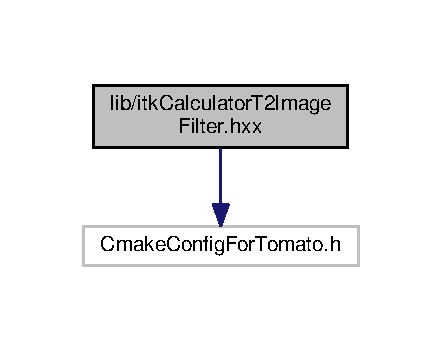
\includegraphics[width=212pt]{itk_calculator_t2_image_filter_8hxx__incl}
\end{center}
\end{figure}


\subsection{Detailed Description}
\begin{DoxyAuthor}{Author}
Konrad Werys 
\end{DoxyAuthor}
\begin{DoxyDate}{Date}
2019/11/08 
\end{DoxyDate}

\hypertarget{_k_w_util_yaml_8h}{\section{lib/\-K\-W\-Util\-Yaml.h File Reference}
\label{_k_w_util_yaml_8h}\index{lib/\-K\-W\-Util\-Yaml.\-h@{lib/\-K\-W\-Util\-Yaml.\-h}}
}
This graph shows which files directly or indirectly include this file\-:
\nopagebreak
\begin{figure}[H]
\begin{center}
\leavevmode
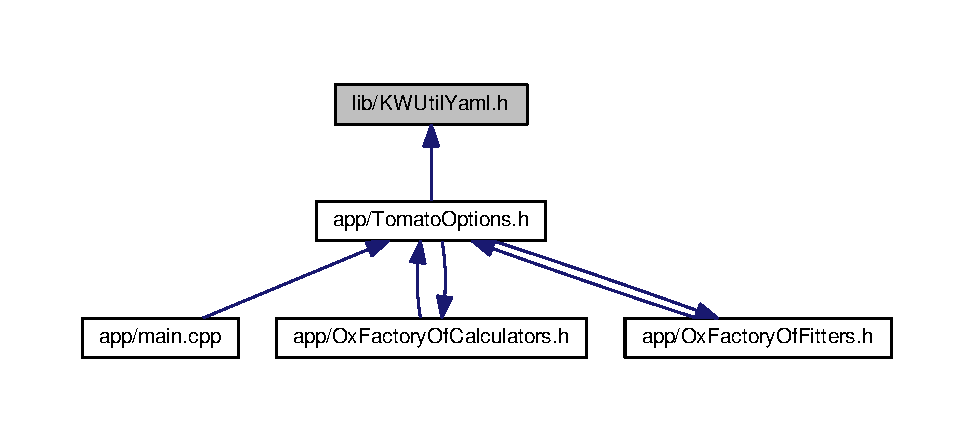
\includegraphics[width=350pt]{_k_w_util_yaml_8h__dep__incl}
\end{center}
\end{figure}
\subsection*{Classes}
\begin{DoxyCompactItemize}
\item 
class \hyperlink{class_k_w_util_yaml}{K\-W\-Util\-Yaml}
\end{DoxyCompactItemize}


\subsection{Detailed Description}
\begin{DoxyAuthor}{Author}
Konrad Werys 
\end{DoxyAuthor}
\begin{DoxyDate}{Date}
2018/11/16 
\end{DoxyDate}

\hypertarget{_ox_calculator_8h}{\section{lib/\-Ox\-Calculator.h File Reference}
\label{_ox_calculator_8h}\index{lib/\-Ox\-Calculator.\-h@{lib/\-Ox\-Calculator.\-h}}
}
{\ttfamily \#include \char`\"{}tomatolib\-\_\-export.\-h\char`\"{}}\\*
{\ttfamily \#include \char`\"{}Ox\-Fitter.\-h\char`\"{}}\\*
{\ttfamily \#include \char`\"{}Ox\-Model.\-h\char`\"{}}\\*
{\ttfamily \#include \char`\"{}Ox\-Sign\-Calculator.\-h\char`\"{}}\\*
{\ttfamily \#include \char`\"{}Ox\-Start\-Point\-Calculator.\-h\char`\"{}}\\*
{\ttfamily \#include $<$map$>$}\\*
{\ttfamily \#include \char`\"{}K\-W\-Util.\-h\char`\"{}}\\*
{\ttfamily \#include \char`\"{}Ox\-Calculator.\-hxx\char`\"{}}\\*
Include dependency graph for Ox\-Calculator.\-h\-:
\nopagebreak
\begin{figure}[H]
\begin{center}
\leavevmode
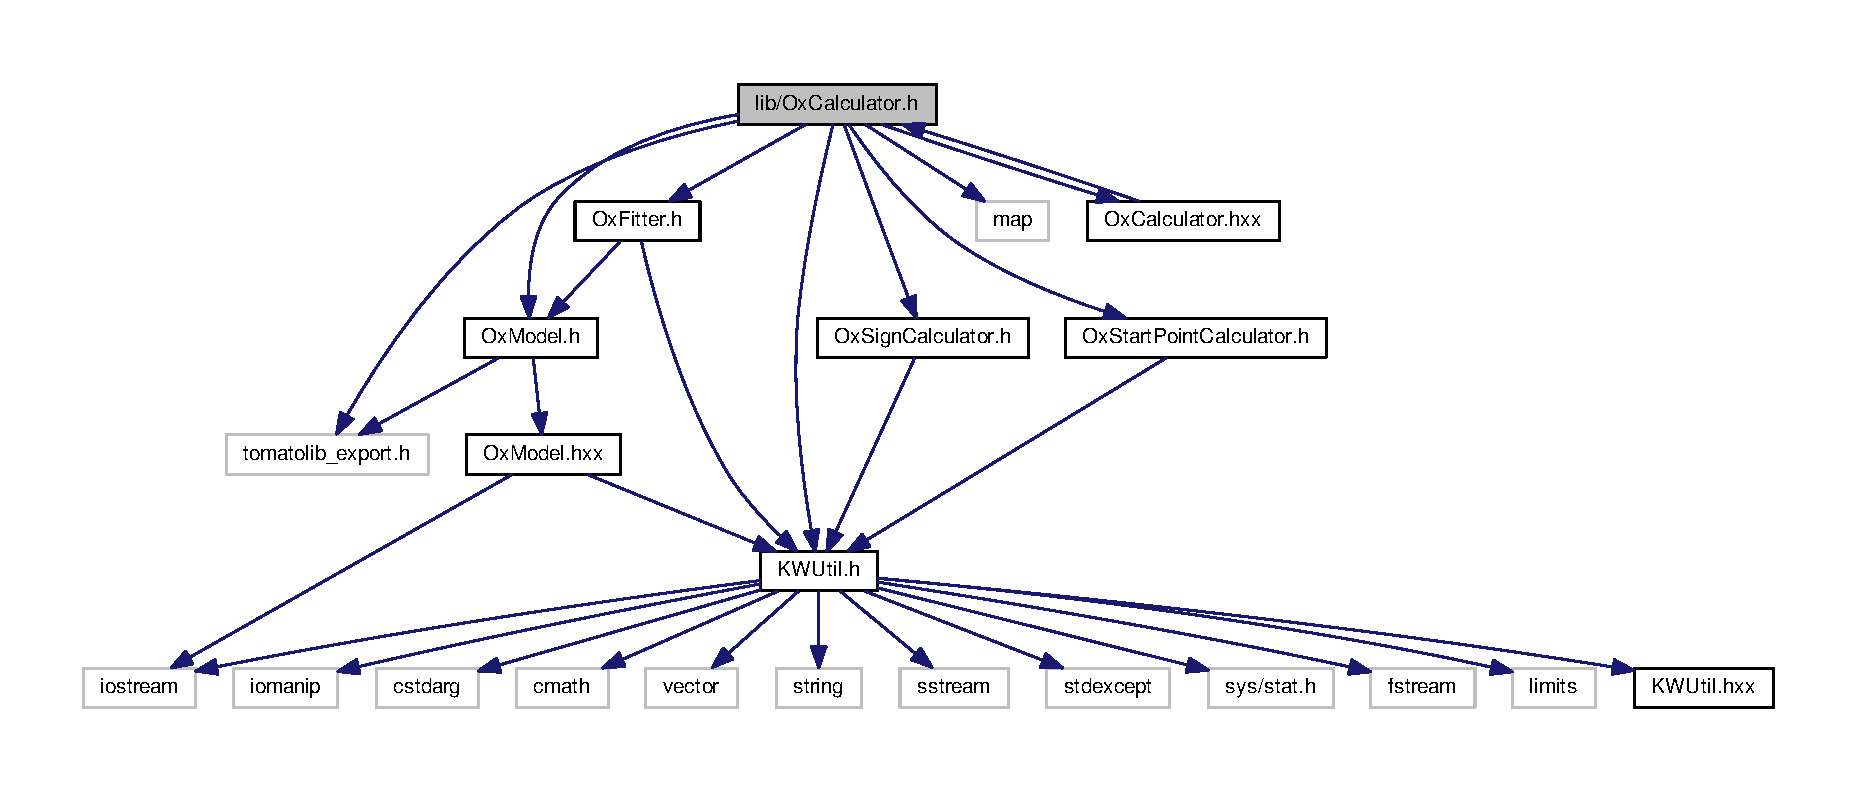
\includegraphics[width=350pt]{_ox_calculator_8h__incl}
\end{center}
\end{figure}
This graph shows which files directly or indirectly include this file\-:
\nopagebreak
\begin{figure}[H]
\begin{center}
\leavevmode
\includegraphics[width=350pt]{_ox_calculator_8h__dep__incl}
\end{center}
\end{figure}
\subsection*{Classes}
\begin{DoxyCompactItemize}
\item 
class \hyperlink{class_ox_1_1_calculator}{Ox\-::\-Calculator$<$ Measure\-Type $>$}
\end{DoxyCompactItemize}


\subsection{Detailed Description}
\begin{DoxyAuthor}{Author}
Konrad Werys 
\end{DoxyAuthor}
\begin{DoxyDate}{Date}
2018/07/29 
\end{DoxyDate}

\hypertarget{_ox_calculator_8hxx}{\section{lib/\-Ox\-Calculator.hxx File Reference}
\label{_ox_calculator_8hxx}\index{lib/\-Ox\-Calculator.\-hxx@{lib/\-Ox\-Calculator.\-hxx}}
}
This graph shows which files directly or indirectly include this file\-:
\nopagebreak
\begin{figure}[H]
\begin{center}
\leavevmode
\includegraphics[width=350pt]{_ox_calculator_8hxx__dep__incl}
\end{center}
\end{figure}


\subsection{Detailed Description}
\begin{DoxyAuthor}{Author}
Konrad Werys 
\end{DoxyAuthor}
\begin{DoxyDate}{Date}
2018/08/09 
\end{DoxyDate}

\hypertarget{_ox_calculator_t1_molli_8h}{\section{lib/\-Ox\-Calculator\-T1\-Molli.h File Reference}
\label{_ox_calculator_t1_molli_8h}\index{lib/\-Ox\-Calculator\-T1\-Molli.\-h@{lib/\-Ox\-Calculator\-T1\-Molli.\-h}}
}
{\ttfamily \#include \char`\"{}Ox\-Calculator\-T1.\-h\char`\"{}}\\*
Include dependency graph for Ox\-Calculator\-T1\-Molli.\-h\-:
\nopagebreak
\begin{figure}[H]
\begin{center}
\leavevmode
\includegraphics[width=350pt]{_ox_calculator_t1_molli_8h__incl}
\end{center}
\end{figure}
This graph shows which files directly or indirectly include this file\-:
\nopagebreak
\begin{figure}[H]
\begin{center}
\leavevmode
\includegraphics[width=210pt]{_ox_calculator_t1_molli_8h__dep__incl}
\end{center}
\end{figure}
\subsection*{Classes}
\begin{DoxyCompactItemize}
\item 
class \hyperlink{class_ox_1_1_calculator_t1_molli}{Ox\-::\-Calculator\-T1\-Molli$<$ Measure\-Type $>$}
\end{DoxyCompactItemize}


\subsection{Detailed Description}
\begin{DoxyAuthor}{Author}
Konrad Werys 
\end{DoxyAuthor}
\begin{DoxyDate}{Date}
2018/08/01 
\end{DoxyDate}

\hypertarget{_ox_calculator_t1_molli_8hxx}{\section{lib/\-Ox\-Calculator\-T1\-Molli.hxx File Reference}
\label{_ox_calculator_t1_molli_8hxx}\index{lib/\-Ox\-Calculator\-T1\-Molli.\-hxx@{lib/\-Ox\-Calculator\-T1\-Molli.\-hxx}}
}
This graph shows which files directly or indirectly include this file\-:
\nopagebreak
\begin{figure}[H]
\begin{center}
\leavevmode
\includegraphics[width=350pt]{_ox_calculator_t1_molli_8hxx__dep__incl}
\end{center}
\end{figure}


\subsection{Detailed Description}
\begin{DoxyAuthor}{Author}
Konrad Werys 
\end{DoxyAuthor}
\begin{DoxyDate}{Date}
2019/01/15 
\end{DoxyDate}

\hypertarget{_ox_calculator_t1_shmolli_8h}{\section{lib/\-Ox\-Calculator\-T1\-Shmolli.h File Reference}
\label{_ox_calculator_t1_shmolli_8h}\index{lib/\-Ox\-Calculator\-T1\-Shmolli.\-h@{lib/\-Ox\-Calculator\-T1\-Shmolli.\-h}}
}
{\ttfamily \#include \char`\"{}tomatolib\-\_\-export.\-h\char`\"{}}\\*
{\ttfamily \#include \char`\"{}Ox\-Calculator\-T1\-With\-Sign\-Check.\-h\char`\"{}}\\*
{\ttfamily \#include \char`\"{}Ox\-Calculator\-T1\-Shmolli.\-hxx\char`\"{}}\\*
Include dependency graph for Ox\-Calculator\-T1\-Shmolli.\-h\-:
\nopagebreak
\begin{figure}[H]
\begin{center}
\leavevmode
\includegraphics[width=350pt]{_ox_calculator_t1_shmolli_8h__incl}
\end{center}
\end{figure}
This graph shows which files directly or indirectly include this file\-:
\nopagebreak
\begin{figure}[H]
\begin{center}
\leavevmode
\includegraphics[width=350pt]{_ox_calculator_t1_shmolli_8h__dep__incl}
\end{center}
\end{figure}
\subsection*{Classes}
\begin{DoxyCompactItemize}
\item 
class \hyperlink{class_ox_1_1_calculator_t1_shmolli}{Ox\-::\-Calculator\-T1\-Shmolli$<$ Measure\-Type $>$}
\end{DoxyCompactItemize}


\subsection{Detailed Description}
\begin{DoxyAuthor}{Author}
Konrad Werys 
\end{DoxyAuthor}
\begin{DoxyDate}{Date}
2018/08/02 
\end{DoxyDate}

\hypertarget{_ox_calculator_t1_shmolli_8hxx}{\section{lib/\-Ox\-Calculator\-T1\-Shmolli.hxx File Reference}
\label{_ox_calculator_t1_shmolli_8hxx}\index{lib/\-Ox\-Calculator\-T1\-Shmolli.\-hxx@{lib/\-Ox\-Calculator\-T1\-Shmolli.\-hxx}}
}
This graph shows which files directly or indirectly include this file\-:
\nopagebreak
\begin{figure}[H]
\begin{center}
\leavevmode
\includegraphics[width=350pt]{_ox_calculator_t1_shmolli_8hxx__dep__incl}
\end{center}
\end{figure}


\subsection{Detailed Description}
\begin{DoxyAuthor}{Author}
Konrad Werys 
\end{DoxyAuthor}
\begin{DoxyDate}{Date}
2019/01/17 
\end{DoxyDate}

\hypertarget{_ox_calculator_t2_8h}{\section{lib/\-Ox\-Calculator\-T2.h File Reference}
\label{_ox_calculator_t2_8h}\index{lib/\-Ox\-Calculator\-T2.\-h@{lib/\-Ox\-Calculator\-T2.\-h}}
}
{\ttfamily \#include \char`\"{}Ox\-Calculator.\-h\char`\"{}}\\*
{\ttfamily \#include \char`\"{}tomatolib\-\_\-export.\-h\char`\"{}}\\*
{\ttfamily \#include \char`\"{}Ox\-Calculator\-T2.\-hxx\char`\"{}}\\*
Include dependency graph for Ox\-Calculator\-T2.\-h\-:
\nopagebreak
\begin{figure}[H]
\begin{center}
\leavevmode
\includegraphics[width=350pt]{_ox_calculator_t2_8h__incl}
\end{center}
\end{figure}
This graph shows which files directly or indirectly include this file\-:
\nopagebreak
\begin{figure}[H]
\begin{center}
\leavevmode
\includegraphics[width=350pt]{_ox_calculator_t2_8h__dep__incl}
\end{center}
\end{figure}
\subsection*{Classes}
\begin{DoxyCompactItemize}
\item 
class \hyperlink{class_ox_1_1_calculator_t2}{Ox\-::\-Calculator\-T2$<$ Measure\-Type $>$}
\end{DoxyCompactItemize}


\subsection{Detailed Description}
\begin{DoxyAuthor}{Author}
Konrad Werys 
\end{DoxyAuthor}
\begin{DoxyDate}{Date}
2019/11/05 
\end{DoxyDate}

\hypertarget{_ox_calculator_t2_8hxx}{\section{lib/\-Ox\-Calculator\-T2.hxx File Reference}
\label{_ox_calculator_t2_8hxx}\index{lib/\-Ox\-Calculator\-T2.\-hxx@{lib/\-Ox\-Calculator\-T2.\-hxx}}
}
This graph shows which files directly or indirectly include this file\-:
\nopagebreak
\begin{figure}[H]
\begin{center}
\leavevmode
\includegraphics[width=194pt]{_ox_calculator_t2_8hxx__dep__incl}
\end{center}
\end{figure}


\subsection{Detailed Description}
\begin{DoxyAuthor}{Author}
Konrad Werys 
\end{DoxyAuthor}
\begin{DoxyDate}{Date}
2019/11/05 
\end{DoxyDate}

\hypertarget{_ox_fitter_8h}{\section{lib/\-Ox\-Fitter.h File Reference}
\label{_ox_fitter_8h}\index{lib/\-Ox\-Fitter.\-h@{lib/\-Ox\-Fitter.\-h}}
}
{\ttfamily \#include \char`\"{}Ox\-Functions\-T1.\-h\char`\"{}}\\*
{\ttfamily \#include \char`\"{}K\-W\-Util.\-h\char`\"{}}\\*
Include dependency graph for Ox\-Fitter.\-h\-:
\nopagebreak
\begin{figure}[H]
\begin{center}
\leavevmode
\includegraphics[width=350pt]{_ox_fitter_8h__incl}
\end{center}
\end{figure}
This graph shows which files directly or indirectly include this file\-:
\nopagebreak
\begin{figure}[H]
\begin{center}
\leavevmode
\includegraphics[width=350pt]{_ox_fitter_8h__dep__incl}
\end{center}
\end{figure}
\subsection*{Classes}
\begin{DoxyCompactItemize}
\item 
class \hyperlink{class_ox_1_1_fitter}{Ox\-::\-Fitter$<$ Measure\-Type $>$}
\end{DoxyCompactItemize}


\subsection{Detailed Description}
\begin{DoxyAuthor}{Author}
Konrad Werys 
\end{DoxyAuthor}
\begin{DoxyDate}{Date}
2018/07/29 
\end{DoxyDate}

\hypertarget{_ox_fitter_amoeba_nr2_8h}{\section{lib/\-Ox\-Fitter\-Amoeba\-Nr2.h File Reference}
\label{_ox_fitter_amoeba_nr2_8h}\index{lib/\-Ox\-Fitter\-Amoeba\-Nr2.\-h@{lib/\-Ox\-Fitter\-Amoeba\-Nr2.\-h}}
}
{\ttfamily \#include \char`\"{}Cmake\-Config\-For\-Tomato.\-h\char`\"{}}\\*
Include dependency graph for Ox\-Fitter\-Amoeba\-Nr2.\-h\-:
\nopagebreak
\begin{figure}[H]
\begin{center}
\leavevmode
\includegraphics[width=212pt]{_ox_fitter_amoeba_nr2_8h__incl}
\end{center}
\end{figure}


\subsection{Detailed Description}
\begin{DoxyAuthor}{Author}
Konrad Werys 
\end{DoxyAuthor}
\begin{DoxyDate}{Date}
2018/08/06 
\end{DoxyDate}

\hypertarget{_ox_fitter_amoeba_vnl_8h}{\section{lib/\-Ox\-Fitter\-Amoeba\-Vnl.h File Reference}
\label{_ox_fitter_amoeba_vnl_8h}\index{lib/\-Ox\-Fitter\-Amoeba\-Vnl.\-h@{lib/\-Ox\-Fitter\-Amoeba\-Vnl.\-h}}
}
{\ttfamily \#include \char`\"{}Cmake\-Config\-For\-Tomato.\-h\char`\"{}}\\*
Include dependency graph for Ox\-Fitter\-Amoeba\-Vnl.\-h\-:
\nopagebreak
\begin{figure}[H]
\begin{center}
\leavevmode
\includegraphics[width=212pt]{_ox_fitter_amoeba_vnl_8h__incl}
\end{center}
\end{figure}
This graph shows which files directly or indirectly include this file\-:
\nopagebreak
\begin{figure}[H]
\begin{center}
\leavevmode
\includegraphics[width=350pt]{_ox_fitter_amoeba_vnl_8h__dep__incl}
\end{center}
\end{figure}


\subsection{Detailed Description}
\begin{DoxyAuthor}{Author}
Konrad Werys 
\end{DoxyAuthor}
\begin{DoxyDate}{Date}
2018/07/30 
\end{DoxyDate}

\hypertarget{_ox_fitter_levenberg_marquardt_lmfit_8h}{}\section{lib/\+Ox\+Fitter\+Levenberg\+Marquardt\+Lmfit.h File Reference}
\label{_ox_fitter_levenberg_marquardt_lmfit_8h}\index{lib/\+Ox\+Fitter\+Levenberg\+Marquardt\+Lmfit.\+h@{lib/\+Ox\+Fitter\+Levenberg\+Marquardt\+Lmfit.\+h}}
{\ttfamily \#include \char`\"{}Cmake\+Config\+For\+Tomato.\+h\char`\"{}}\\*
Include dependency graph for Ox\+Fitter\+Levenberg\+Marquardt\+Lmfit.\+h\+:
\nopagebreak
\begin{figure}[H]
\begin{center}
\leavevmode
\includegraphics[width=233pt]{_ox_fitter_levenberg_marquardt_lmfit_8h__incl}
\end{center}
\end{figure}
This graph shows which files directly or indirectly include this file\+:
\nopagebreak
\begin{figure}[H]
\begin{center}
\leavevmode
\includegraphics[width=233pt]{_ox_fitter_levenberg_marquardt_lmfit_8h__dep__incl}
\end{center}
\end{figure}


\subsection{Detailed Description}
\begin{DoxyAuthor}{Author}
Konrad Werys 
\end{DoxyAuthor}
\begin{DoxyDate}{Date}
2019/08/14
\end{DoxyDate}
\begin{DoxyAuthor}{Author}
Konrad Werys 
\end{DoxyAuthor}
\begin{DoxyDate}{Date}
2020/10/23 
\end{DoxyDate}

\hypertarget{_ox_fitter_levenberg_marquardt_vnl_8h}{\section{lib/\-Ox\-Fitter\-Levenberg\-Marquardt\-Vnl.h File Reference}
\label{_ox_fitter_levenberg_marquardt_vnl_8h}\index{lib/\-Ox\-Fitter\-Levenberg\-Marquardt\-Vnl.\-h@{lib/\-Ox\-Fitter\-Levenberg\-Marquardt\-Vnl.\-h}}
}
{\ttfamily \#include \char`\"{}Ox\-Fitter.\-h\char`\"{}}\\*
{\ttfamily \#include \char`\"{}Ox\-Functions\-T1\-Adapter\-Vnl\-Least\-Squares.\-h\char`\"{}}\\*
{\ttfamily \#include $<$vnl/algo/vnl\-\_\-levenberg\-\_\-marquardt.\-h$>$}\\*
Include dependency graph for Ox\-Fitter\-Levenberg\-Marquardt\-Vnl.\-h\-:
\nopagebreak
\begin{figure}[H]
\begin{center}
\leavevmode
\includegraphics[width=350pt]{_ox_fitter_levenberg_marquardt_vnl_8h__incl}
\end{center}
\end{figure}
This graph shows which files directly or indirectly include this file\-:
\nopagebreak
\begin{figure}[H]
\begin{center}
\leavevmode
\includegraphics[width=350pt]{_ox_fitter_levenberg_marquardt_vnl_8h__dep__incl}
\end{center}
\end{figure}
\subsection*{Classes}
\begin{DoxyCompactItemize}
\item 
class \hyperlink{class_ox_1_1_fitter_levenberg_marquardt_vnl}{Ox\-::\-Fitter\-Levenberg\-Marquardt\-Vnl$<$ Measure\-Type $>$}
\end{DoxyCompactItemize}


\subsection{Detailed Description}
\begin{DoxyAuthor}{Author}
Konrad Werys 
\end{DoxyAuthor}
\begin{DoxyDate}{Date}
2018/07/31 
\end{DoxyDate}

\hypertarget{_ox_model_8h}{}\section{lib/\+Ox\+Model.h File Reference}
\label{_ox_model_8h}\index{lib/\+Ox\+Model.\+h@{lib/\+Ox\+Model.\+h}}
{\ttfamily \#include \char`\"{}tomatolib\+\_\+export.\+h\char`\"{}}\\*
{\ttfamily \#include $<$string$>$}\\*
{\ttfamily \#include \char`\"{}Ox\+Model.\+hxx\char`\"{}}\\*
Include dependency graph for Ox\+Model.\+h\+:
\nopagebreak
\begin{figure}[H]
\begin{center}
\leavevmode
\includegraphics[width=350pt]{_ox_model_8h__incl}
\end{center}
\end{figure}
This graph shows which files directly or indirectly include this file\+:
\nopagebreak
\begin{figure}[H]
\begin{center}
\leavevmode
\includegraphics[width=350pt]{_ox_model_8h__dep__incl}
\end{center}
\end{figure}
\subsection*{Classes}
\begin{DoxyCompactItemize}
\item 
class \hyperlink{class_ox_1_1_model}{Ox\+::\+Model$<$ Measure\+Type $>$}
\begin{DoxyCompactList}\small\item\em Container for a model function, cost function and Least-\/\+Squares function. And derivatives. \end{DoxyCompactList}\end{DoxyCompactItemize}


\subsection{Detailed Description}
\begin{DoxyAuthor}{Author}
Konrad Werys 
\end{DoxyAuthor}
\begin{DoxyDate}{Date}
2018/07/29 
\end{DoxyDate}

\hypertarget{_ox_model_t1_adapter_lmfit_least_squares_8h}{\section{lib/\-Ox\-Model\-T1\-Adapter\-Lmfit\-Least\-Squares.h File Reference}
\label{_ox_model_t1_adapter_lmfit_least_squares_8h}\index{lib/\-Ox\-Model\-T1\-Adapter\-Lmfit\-Least\-Squares.\-h@{lib/\-Ox\-Model\-T1\-Adapter\-Lmfit\-Least\-Squares.\-h}}
}
{\ttfamily \#include \char`\"{}Cmake\-Config\-For\-Tomato.\-h\char`\"{}}\\*
Include dependency graph for Ox\-Model\-T1\-Adapter\-Lmfit\-Least\-Squares.\-h\-:
\nopagebreak
\begin{figure}[H]
\begin{center}
\leavevmode
\includegraphics[width=214pt]{_ox_model_t1_adapter_lmfit_least_squares_8h__incl}
\end{center}
\end{figure}


\subsection{Detailed Description}
\begin{DoxyAuthor}{Author}
Konrad Werys 
\end{DoxyAuthor}
\begin{DoxyDate}{Date}
2019/08/15 
\end{DoxyDate}

\hypertarget{_ox_model_t1_adapter_vnl_cost_8h}{}\section{lib/\+Ox\+Model\+T1\+Adapter\+Vnl\+Cost.h File Reference}
\label{_ox_model_t1_adapter_vnl_cost_8h}\index{lib/\+Ox\+Model\+T1\+Adapter\+Vnl\+Cost.\+h@{lib/\+Ox\+Model\+T1\+Adapter\+Vnl\+Cost.\+h}}
{\ttfamily \#include \char`\"{}Cmake\+Config\+For\+Tomato.\+h\char`\"{}}\\*
Include dependency graph for Ox\+Model\+T1\+Adapter\+Vnl\+Cost.\+h\+:
\nopagebreak
\begin{figure}[H]
\begin{center}
\leavevmode
\includegraphics[width=237pt]{_ox_model_t1_adapter_vnl_cost_8h__incl}
\end{center}
\end{figure}


\subsection{Detailed Description}
\begin{DoxyAuthor}{Author}
Konrad Werys 
\end{DoxyAuthor}
\begin{DoxyDate}{Date}
2018/07/30 
\end{DoxyDate}

\hypertarget{_ox_model_t1_adapter_vnl_least_squares_8h}{}\section{lib/\+Ox\+Model\+T1\+Adapter\+Vnl\+Least\+Squares.h File Reference}
\label{_ox_model_t1_adapter_vnl_least_squares_8h}\index{lib/\+Ox\+Model\+T1\+Adapter\+Vnl\+Least\+Squares.\+h@{lib/\+Ox\+Model\+T1\+Adapter\+Vnl\+Least\+Squares.\+h}}
{\ttfamily \#include \char`\"{}Cmake\+Config\+For\+Tomato.\+h\char`\"{}}\\*
Include dependency graph for Ox\+Model\+T1\+Adapter\+Vnl\+Least\+Squares.\+h\+:
\nopagebreak
\begin{figure}[H]
\begin{center}
\leavevmode
\includegraphics[width=232pt]{_ox_model_t1_adapter_vnl_least_squares_8h__incl}
\end{center}
\end{figure}


\subsection{Detailed Description}
\begin{DoxyAuthor}{Author}
Konrad Werys 
\end{DoxyAuthor}
\begin{DoxyDate}{Date}
2018/07/30 
\end{DoxyDate}

\hypertarget{_ox_model_t1_shmolli_8h}{\section{lib/\-Ox\-Model\-T1\-Shmolli.h File Reference}
\label{_ox_model_t1_shmolli_8h}\index{lib/\-Ox\-Model\-T1\-Shmolli.\-h@{lib/\-Ox\-Model\-T1\-Shmolli.\-h}}
}
{\ttfamily \#include \char`\"{}tomatolib\-\_\-export.\-h\char`\"{}}\\*
{\ttfamily \#include \char`\"{}Ox\-Model.\-h\char`\"{}}\\*
{\ttfamily \#include $<$cmath$>$}\\*
{\ttfamily \#include \char`\"{}Ox\-Model\-T1\-Shmolli.\-hxx\char`\"{}}\\*
Include dependency graph for Ox\-Model\-T1\-Shmolli.\-h\-:
\nopagebreak
\begin{figure}[H]
\begin{center}
\leavevmode
\includegraphics[width=350pt]{_ox_model_t1_shmolli_8h__incl}
\end{center}
\end{figure}
This graph shows which files directly or indirectly include this file\-:
\nopagebreak
\begin{figure}[H]
\begin{center}
\leavevmode
\includegraphics[width=302pt]{_ox_model_t1_shmolli_8h__dep__incl}
\end{center}
\end{figure}
\subsection*{Classes}
\begin{DoxyCompactItemize}
\item 
class \hyperlink{class_ox_1_1_model_t1_shmolli}{Ox\-::\-Model\-T1\-Shmolli$<$ Measure\-Type $>$}
\begin{DoxyCompactList}\small\item\em Container for a Calculator\-Shmolli model function $ A-B\exp(t/T_1^*) $, cost function and Least-\/\-Squares function and derivatives. \end{DoxyCompactList}\end{DoxyCompactItemize}


\subsection{Detailed Description}
\begin{DoxyAuthor}{Author}
Konrad Werys 
\end{DoxyAuthor}
\begin{DoxyDate}{Date}
2018/08/22 
\end{DoxyDate}

\hypertarget{_ox_model_t1_shmolli_8hxx}{\section{lib/\-Ox\-Model\-T1\-Shmolli.hxx File Reference}
\label{_ox_model_t1_shmolli_8hxx}\index{lib/\-Ox\-Model\-T1\-Shmolli.\-hxx@{lib/\-Ox\-Model\-T1\-Shmolli.\-hxx}}
}
This graph shows which files directly or indirectly include this file\-:
\nopagebreak
\begin{figure}[H]
\begin{center}
\leavevmode
\includegraphics[width=308pt]{_ox_model_t1_shmolli_8hxx__dep__incl}
\end{center}
\end{figure}


\subsection{Detailed Description}
\begin{DoxyAuthor}{Author}
Konrad Werys 
\end{DoxyAuthor}
\begin{DoxyDate}{Date}
2018/08/22 
\end{DoxyDate}

\hypertarget{_ox_model_t1_three_param_8h}{}\section{lib/\+Ox\+Model\+T1\+Three\+Param.h File Reference}
\label{_ox_model_t1_three_param_8h}\index{lib/\+Ox\+Model\+T1\+Three\+Param.\+h@{lib/\+Ox\+Model\+T1\+Three\+Param.\+h}}
{\ttfamily \#include \char`\"{}tomatolib\+\_\+export.\+h\char`\"{}}\\*
{\ttfamily \#include \char`\"{}Ox\+Model.\+h\char`\"{}}\\*
{\ttfamily \#include $<$cmath$>$}\\*
{\ttfamily \#include \char`\"{}Ox\+Model\+T1\+Three\+Param.\+hxx\char`\"{}}\\*
Include dependency graph for Ox\+Model\+T1\+Three\+Param.\+h\+:
\nopagebreak
\begin{figure}[H]
\begin{center}
\leavevmode
\includegraphics[width=350pt]{_ox_model_t1_three_param_8h__incl}
\end{center}
\end{figure}
This graph shows which files directly or indirectly include this file\+:
\nopagebreak
\begin{figure}[H]
\begin{center}
\leavevmode
\includegraphics[width=350pt]{_ox_model_t1_three_param_8h__dep__incl}
\end{center}
\end{figure}
\subsection*{Classes}
\begin{DoxyCompactItemize}
\item 
class \hyperlink{class_ox_1_1_model_t1_three_param}{Ox\+::\+Model\+T1\+Three\+Param$<$ Measure\+Type $>$}
\begin{DoxyCompactList}\small\item\em Container for a Three\+Param model function $ A-B\exp(t/T_1^*) $, cost function and Least-\/\+Squares function and derivatives. \end{DoxyCompactList}\end{DoxyCompactItemize}


\subsection{Detailed Description}
\begin{DoxyAuthor}{Author}
Konrad Werys 
\end{DoxyAuthor}
\begin{DoxyDate}{Date}
2018/07/29 
\end{DoxyDate}

\hypertarget{_ox_model_t1_three_param_8hxx}{\section{lib/\-Ox\-Model\-T1\-Three\-Param.hxx File Reference}
\label{_ox_model_t1_three_param_8hxx}\index{lib/\-Ox\-Model\-T1\-Three\-Param.\-hxx@{lib/\-Ox\-Model\-T1\-Three\-Param.\-hxx}}
}
This graph shows which files directly or indirectly include this file\-:
\nopagebreak
\begin{figure}[H]
\begin{center}
\leavevmode
\includegraphics[width=350pt]{_ox_model_t1_three_param_8hxx__dep__incl}
\end{center}
\end{figure}


\subsection{Detailed Description}
\begin{DoxyAuthor}{Author}
Konrad Werys 
\end{DoxyAuthor}
\begin{DoxyDate}{Date}
2018/07/29 
\end{DoxyDate}

\hypertarget{_ox_model_t1_two_param_8h}{}\section{lib/\+Ox\+Model\+T1\+Two\+Param.h File Reference}
\label{_ox_model_t1_two_param_8h}\index{lib/\+Ox\+Model\+T1\+Two\+Param.\+h@{lib/\+Ox\+Model\+T1\+Two\+Param.\+h}}
{\ttfamily \#include \char`\"{}tomatolib\+\_\+export.\+h\char`\"{}}\\*
{\ttfamily \#include \char`\"{}Ox\+Model.\+h\char`\"{}}\\*
{\ttfamily \#include $<$cmath$>$}\\*
{\ttfamily \#include \char`\"{}Ox\+Model\+T1\+Two\+Param.\+hxx\char`\"{}}\\*
Include dependency graph for Ox\+Model\+T1\+Two\+Param.\+h\+:
\nopagebreak
\begin{figure}[H]
\begin{center}
\leavevmode
\includegraphics[width=350pt]{_ox_model_t1_two_param_8h__incl}
\end{center}
\end{figure}
This graph shows which files directly or indirectly include this file\+:
\nopagebreak
\begin{figure}[H]
\begin{center}
\leavevmode
\includegraphics[width=350pt]{_ox_model_t1_two_param_8h__dep__incl}
\end{center}
\end{figure}
\subsection*{Classes}
\begin{DoxyCompactItemize}
\item 
class \hyperlink{class_ox_1_1_model_t1_two_param}{Ox\+::\+Model\+T1\+Two\+Param$<$ Measure\+Type $>$}
\begin{DoxyCompactList}\small\item\em Container for a Two\+Param model function $ A(1 - exp( -time / T1 )) $, cost function and Least-\/\+Squares function and derivatives. \end{DoxyCompactList}\end{DoxyCompactItemize}


\subsection{Detailed Description}
\begin{DoxyAuthor}{Author}
Konrad Werys 
\end{DoxyAuthor}
\begin{DoxyDate}{Date}
2018/07/29 
\end{DoxyDate}

\hypertarget{_ox_model_t1_two_param_8hxx}{\section{lib/\-Ox\-Model\-T1\-Two\-Param.hxx File Reference}
\label{_ox_model_t1_two_param_8hxx}\index{lib/\-Ox\-Model\-T1\-Two\-Param.\-hxx@{lib/\-Ox\-Model\-T1\-Two\-Param.\-hxx}}
}
This graph shows which files directly or indirectly include this file\-:
\nopagebreak
\begin{figure}[H]
\begin{center}
\leavevmode
\includegraphics[width=350pt]{_ox_model_t1_two_param_8hxx__dep__incl}
\end{center}
\end{figure}


\subsection{Detailed Description}
\begin{DoxyAuthor}{Author}
Konrad Werys 
\end{DoxyAuthor}
\begin{DoxyDate}{Date}
2018/07/29 
\end{DoxyDate}

\hypertarget{_ox_model_t2_three_param_8h}{\section{lib/\-Ox\-Model\-T2\-Three\-Param.h File Reference}
\label{_ox_model_t2_three_param_8h}\index{lib/\-Ox\-Model\-T2\-Three\-Param.\-h@{lib/\-Ox\-Model\-T2\-Three\-Param.\-h}}
}
{\ttfamily \#include \char`\"{}tomatolib\-\_\-export.\-h\char`\"{}}\\*
{\ttfamily \#include \char`\"{}Ox\-Model.\-h\char`\"{}}\\*
{\ttfamily \#include $<$cmath$>$}\\*
{\ttfamily \#include \char`\"{}Ox\-Model\-T2\-Three\-Param.\-hxx\char`\"{}}\\*
Include dependency graph for Ox\-Model\-T2\-Three\-Param.\-h\-:
\nopagebreak
\begin{figure}[H]
\begin{center}
\leavevmode
\includegraphics[width=350pt]{_ox_model_t2_three_param_8h__incl}
\end{center}
\end{figure}
This graph shows which files directly or indirectly include this file\-:
\nopagebreak
\begin{figure}[H]
\begin{center}
\leavevmode
\includegraphics[width=350pt]{_ox_model_t2_three_param_8h__dep__incl}
\end{center}
\end{figure}
\subsection*{Classes}
\begin{DoxyCompactItemize}
\item 
class \hyperlink{class_ox_1_1_model_t2_three_param}{Ox\-::\-Model\-T2\-Three\-Param$<$ Measure\-Type $>$}
\begin{DoxyCompactList}\small\item\em Container for a Three\-Param model function $ A + B\exp(t/T_2) $, cost function and Least-\/\-Squares function and derivatives. \end{DoxyCompactList}\end{DoxyCompactItemize}


\subsection{Detailed Description}
\begin{DoxyAuthor}{Author}
Konrad Werys 
\end{DoxyAuthor}
\begin{DoxyDate}{Date}
2019/11/04 
\end{DoxyDate}

\hypertarget{_ox_model_t2_three_param_8hxx}{\section{lib/\-Ox\-Model\-T2\-Three\-Param.hxx File Reference}
\label{_ox_model_t2_three_param_8hxx}\index{lib/\-Ox\-Model\-T2\-Three\-Param.\-hxx@{lib/\-Ox\-Model\-T2\-Three\-Param.\-hxx}}
}
This graph shows which files directly or indirectly include this file\-:
\nopagebreak
\begin{figure}[H]
\begin{center}
\leavevmode
\includegraphics[width=350pt]{_ox_model_t2_three_param_8hxx__dep__incl}
\end{center}
\end{figure}


\subsection{Detailed Description}
\begin{DoxyAuthor}{Author}
Konrad Werys 
\end{DoxyAuthor}
\begin{DoxyDate}{Date}
2019/11/04 
\end{DoxyDate}

\hypertarget{_ox_sign_calculator_8h}{}\section{lib/\+Ox\+Sign\+Calculator.h File Reference}
\label{_ox_sign_calculator_8h}\index{lib/\+Ox\+Sign\+Calculator.\+h@{lib/\+Ox\+Sign\+Calculator.\+h}}
This graph shows which files directly or indirectly include this file\+:
% FIG 0
\subsection*{Classes}
\begin{DoxyCompactItemize}
\item 
class \mbox{\hyperlink{class_ox_1_1_sign_calculator}{Ox\+::\+Sign\+Calculator$<$ Measure\+Type $>$}}
\end{DoxyCompactItemize}


\subsection{Detailed Description}
\begin{DoxyAuthor}{Author}
Konrad Werys 
\end{DoxyAuthor}
\begin{DoxyDate}{Date}
2018/08/29 
\end{DoxyDate}

\hypertarget{_ox_sign_calculator_no_sign_8h}{}\section{lib/\+Ox\+Sign\+Calculator\+No\+Sign.h File Reference}
\label{_ox_sign_calculator_no_sign_8h}\index{lib/\+Ox\+Sign\+Calculator\+No\+Sign.\+h@{lib/\+Ox\+Sign\+Calculator\+No\+Sign.\+h}}
{\ttfamily \#include \char`\"{}Ox\+Sign\+Calculator.\+h\char`\"{}}\\*
Include dependency graph for Ox\+Sign\+Calculator\+No\+Sign.\+h\+:
\nopagebreak
\begin{figure}[H]
\begin{center}
\leavevmode
\includegraphics[width=350pt]{_ox_sign_calculator_no_sign_8h__incl}
\end{center}
\end{figure}
This graph shows which files directly or indirectly include this file\+:
\nopagebreak
\begin{figure}[H]
\begin{center}
\leavevmode
\includegraphics[width=350pt]{_ox_sign_calculator_no_sign_8h__dep__incl}
\end{center}
\end{figure}
\subsection*{Classes}
\begin{DoxyCompactItemize}
\item 
class \hyperlink{class_ox_1_1_sign_calculator_no_sign}{Ox\+::\+Sign\+Calculator\+No\+Sign$<$ Measure\+Type $>$}
\end{DoxyCompactItemize}


\subsection{Detailed Description}
\begin{DoxyAuthor}{Author}
Konrad Werys 
\end{DoxyAuthor}
\begin{DoxyDate}{Date}
2018/08/13 
\end{DoxyDate}

\hypertarget{_ox_sign_calculator_real_imag_8h}{\section{lib/\-Ox\-Sign\-Calculator\-Real\-Imag.h File Reference}
\label{_ox_sign_calculator_real_imag_8h}\index{lib/\-Ox\-Sign\-Calculator\-Real\-Imag.\-h@{lib/\-Ox\-Sign\-Calculator\-Real\-Imag.\-h}}
}
{\ttfamily \#include \char`\"{}Ox\-Sign\-Calculator.\-h\char`\"{}}\\*
{\ttfamily \#include \char`\"{}K\-W\-Util.\-h\char`\"{}}\\*
Include dependency graph for Ox\-Sign\-Calculator\-Real\-Imag.\-h\-:
\nopagebreak
\begin{figure}[H]
\begin{center}
\leavevmode
\includegraphics[width=350pt]{_ox_sign_calculator_real_imag_8h__incl}
\end{center}
\end{figure}
This graph shows which files directly or indirectly include this file\-:
\nopagebreak
\begin{figure}[H]
\begin{center}
\leavevmode
\includegraphics[width=350pt]{_ox_sign_calculator_real_imag_8h__dep__incl}
\end{center}
\end{figure}
\subsection*{Classes}
\begin{DoxyCompactItemize}
\item 
class \hyperlink{class_ox_1_1_sign_calculator_real_imag}{Ox\-::\-Sign\-Calculator\-Real\-Imag$<$ Measure\-Type $>$}
\end{DoxyCompactItemize}


\subsection{Detailed Description}
\begin{DoxyAuthor}{Author}
Konrad Werys 
\end{DoxyAuthor}
\begin{DoxyDate}{Date}
2018/08/01 
\end{DoxyDate}

\hypertarget{_ox_sign_calculator_shmolli_8h}{}\section{lib/\+Ox\+Sign\+Calculator\+Shmolli.h File Reference}
\label{_ox_sign_calculator_shmolli_8h}\index{lib/\+Ox\+Sign\+Calculator\+Shmolli.\+h@{lib/\+Ox\+Sign\+Calculator\+Shmolli.\+h}}
{\ttfamily \#include \char`\"{}Ox\+Sign\+Calculator.\+h\char`\"{}}\\*
{\ttfamily \#include \char`\"{}K\+W\+Util.\+h\char`\"{}}\\*
Include dependency graph for Ox\+Sign\+Calculator\+Shmolli.\+h\+:
\nopagebreak
\begin{figure}[H]
\begin{center}
\leavevmode
\includegraphics[width=350pt]{_ox_sign_calculator_shmolli_8h__incl}
\end{center}
\end{figure}
This graph shows which files directly or indirectly include this file\+:
\nopagebreak
\begin{figure}[H]
\begin{center}
\leavevmode
\includegraphics[width=350pt]{_ox_sign_calculator_shmolli_8h__dep__incl}
\end{center}
\end{figure}
\subsection*{Classes}
\begin{DoxyCompactItemize}
\item 
class \hyperlink{class_ox_1_1_sign_calculator_shmolli}{Ox\+::\+Sign\+Calculator\+Shmolli$<$ Measure\+Type $>$}
\end{DoxyCompactItemize}


\subsection{Detailed Description}
\begin{DoxyAuthor}{Author}
Konrad Werys 
\end{DoxyAuthor}
\begin{DoxyDate}{Date}
2018/08/01 
\end{DoxyDate}

\hypertarget{_ox_start_point_calculator_8h}{\section{lib/\-Ox\-Start\-Point\-Calculator.h File Reference}
\label{_ox_start_point_calculator_8h}\index{lib/\-Ox\-Start\-Point\-Calculator.\-h@{lib/\-Ox\-Start\-Point\-Calculator.\-h}}
}
This graph shows which files directly or indirectly include this file\-:
\nopagebreak
\begin{figure}[H]
\begin{center}
\leavevmode
\includegraphics[width=218pt]{_ox_start_point_calculator_8h__dep__incl}
\end{center}
\end{figure}
\subsection*{Classes}
\begin{DoxyCompactItemize}
\item 
class \hyperlink{class_ox_1_1_start_point_calculator}{Ox\-::\-Start\-Point\-Calculator$<$ Measure\-Type $>$}
\end{DoxyCompactItemize}


\subsection{Detailed Description}
\begin{DoxyAuthor}{Author}
Konrad Werys 
\end{DoxyAuthor}
\begin{DoxyDate}{Date}
2018/07/29 
\end{DoxyDate}

\hypertarget{_ox_start_point_calculator_basic_8h}{\section{lib/\-Ox\-Start\-Point\-Calculator\-Basic.h File Reference}
\label{_ox_start_point_calculator_basic_8h}\index{lib/\-Ox\-Start\-Point\-Calculator\-Basic.\-h@{lib/\-Ox\-Start\-Point\-Calculator\-Basic.\-h}}
}
{\ttfamily \#include \char`\"{}Ox\-Start\-Point\-Calculator.\-h\char`\"{}}\\*
Include dependency graph for Ox\-Start\-Point\-Calculator\-Basic.\-h\-:
\nopagebreak
\begin{figure}[H]
\begin{center}
\leavevmode
\includegraphics[width=350pt]{_ox_start_point_calculator_basic_8h__incl}
\end{center}
\end{figure}
This graph shows which files directly or indirectly include this file\-:
\nopagebreak
\begin{figure}[H]
\begin{center}
\leavevmode
\includegraphics[width=350pt]{_ox_start_point_calculator_basic_8h__dep__incl}
\end{center}
\end{figure}
\subsection*{Classes}
\begin{DoxyCompactItemize}
\item 
class \hyperlink{class_ox_1_1_start_point_calculator_basic}{Ox\-::\-Start\-Point\-Calculator\-Basic$<$ Measure\-Type $>$}
\end{DoxyCompactItemize}


\subsection{Detailed Description}
\begin{DoxyAuthor}{Author}
Konrad Werys 
\end{DoxyAuthor}
\begin{DoxyDate}{Date}
2018/08/10 
\end{DoxyDate}

\hypertarget{_ox_start_point_calculator_shmolli_8h}{\section{lib/\-Ox\-Start\-Point\-Calculator\-Shmolli.h File Reference}
\label{_ox_start_point_calculator_shmolli_8h}\index{lib/\-Ox\-Start\-Point\-Calculator\-Shmolli.\-h@{lib/\-Ox\-Start\-Point\-Calculator\-Shmolli.\-h}}
}
{\ttfamily \#include \char`\"{}Ox\-Start\-Point\-Calculator.\-h\char`\"{}}\\*
Include dependency graph for Ox\-Start\-Point\-Calculator\-Shmolli.\-h\-:
\nopagebreak
\begin{figure}[H]
\begin{center}
\leavevmode
\includegraphics[width=350pt]{_ox_start_point_calculator_shmolli_8h__incl}
\end{center}
\end{figure}
This graph shows which files directly or indirectly include this file\-:
\nopagebreak
\begin{figure}[H]
\begin{center}
\leavevmode
\includegraphics[width=350pt]{_ox_start_point_calculator_shmolli_8h__dep__incl}
\end{center}
\end{figure}
\subsection*{Classes}
\begin{DoxyCompactItemize}
\item 
class \hyperlink{class_ox_1_1_start_point_calculator_shmolli}{Ox\-::\-Start\-Point\-Calculator\-Shmolli$<$ Measure\-Type $>$}
\end{DoxyCompactItemize}


\subsection{Detailed Description}
\begin{DoxyAuthor}{Author}
Konrad Werys 
\end{DoxyAuthor}
\begin{DoxyDate}{Date}
2018/08/10 
\end{DoxyDate}

\hypertarget{_tomato_api_8cpp}{}\section{lib/\+Tomato\+Api.cpp File Reference}
\label{_tomato_api_8cpp}\index{lib/\+Tomato\+Api.\+cpp@{lib/\+Tomato\+Api.\+cpp}}
{\ttfamily \#include \char`\"{}Tomato\+Api.\+h\char`\"{}}\\*
Include dependency graph for Tomato\+Api.\+cpp\+:
\nopagebreak
\begin{figure}[H]
\begin{center}
\leavevmode
\includegraphics[width=350pt]{_tomato_api_8cpp__incl}
\end{center}
\end{figure}


\subsection{Detailed Description}
\begin{DoxyAuthor}{Author}
Konrad Werys 
\end{DoxyAuthor}
\begin{DoxyDate}{Date}
2019/01/15 
\end{DoxyDate}

\hypertarget{_tomato_api_8h}{\section{lib/\-Tomato\-Api.h File Reference}
\label{_tomato_api_8h}\index{lib/\-Tomato\-Api.\-h@{lib/\-Tomato\-Api.\-h}}
}
{\ttfamily \#include \char`\"{}Cmake\-Config\-For\-Tomato.\-h\char`\"{}}\\*
{\ttfamily \#include \char`\"{}tomatolib\-\_\-export.\-h\char`\"{}}\\*
{\ttfamily \#include \char`\"{}Ox\-Calculator.\-h\char`\"{}}\\*
{\ttfamily \#include \char`\"{}Ox\-Calculator\-T1\-Molli.\-h\char`\"{}}\\*
{\ttfamily \#include \char`\"{}Ox\-Fitter.\-h\char`\"{}}\\*
{\ttfamily \#include \char`\"{}Ox\-Model.\-h\char`\"{}}\\*
{\ttfamily \#include \char`\"{}Ox\-Model\-T1\-Three\-Param.\-h\char`\"{}}\\*
{\ttfamily \#include \char`\"{}Ox\-Sign\-Calculator.\-h\char`\"{}}\\*
{\ttfamily \#include \char`\"{}Ox\-Sign\-Calculator\-No\-Sign.\-h\char`\"{}}\\*
{\ttfamily \#include \char`\"{}Ox\-Sign\-Calculator\-Real\-Imag.\-h\char`\"{}}\\*
{\ttfamily \#include \char`\"{}Ox\-Start\-Point\-Calculator\-Basic.\-h\char`\"{}}\\*
Include dependency graph for Tomato\-Api.\-h\-:
\nopagebreak
\begin{figure}[H]
\begin{center}
\leavevmode
\includegraphics[width=350pt]{_tomato_api_8h__incl}
\end{center}
\end{figure}
This graph shows which files directly or indirectly include this file\-:
\nopagebreak
\begin{figure}[H]
\begin{center}
\leavevmode
\includegraphics[width=174pt]{_tomato_api_8h__dep__incl}
\end{center}
\end{figure}
\subsection*{Variables}
\begin{DoxyCompactItemize}
\item 
\hypertarget{namespace_ox_a9b8230abbabcc9e797ae3d9844af1bea}{template class T\-O\-M\-A\-T\-O\-L\-I\-B\-\_\-\-E\-X\-P\-O\-R\-T {\bfseries Ox\-::\-Calculator$<$ double $>$}}\label{namespace_ox_a9b8230abbabcc9e797ae3d9844af1bea}

\item 
\hypertarget{namespace_ox_a7d0473f70666fc11f4c370f408240086}{template class T\-O\-M\-A\-T\-O\-L\-I\-B\-\_\-\-E\-X\-P\-O\-R\-T {\bfseries Ox\-::\-Calculator\-T1\-Molli$<$ double $>$}}\label{namespace_ox_a7d0473f70666fc11f4c370f408240086}

\item 
\hypertarget{namespace_ox_a1e4e4356bc0f519c7b33750ff33594f1}{template class T\-O\-M\-A\-T\-O\-L\-I\-B\-\_\-\-E\-X\-P\-O\-R\-T {\bfseries Ox\-::\-Fitter$<$ double $>$}}\label{namespace_ox_a1e4e4356bc0f519c7b33750ff33594f1}

\item 
\hypertarget{namespace_ox_af85883bfc75370cbe7359ce6f2f8f3b4}{template class T\-O\-M\-A\-T\-O\-L\-I\-B\-\_\-\-E\-X\-P\-O\-R\-T {\bfseries Ox\-::\-Model$<$ double $>$}}\label{namespace_ox_af85883bfc75370cbe7359ce6f2f8f3b4}

\item 
\hypertarget{namespace_ox_adab5d5b6b27e41b97f5a0f721da27773}{template class T\-O\-M\-A\-T\-O\-L\-I\-B\-\_\-\-E\-X\-P\-O\-R\-T {\bfseries Ox\-::\-Model\-T1\-Three\-Param$<$ double $>$}}\label{namespace_ox_adab5d5b6b27e41b97f5a0f721da27773}

\item 
\hypertarget{namespace_ox_aef50802c4cb9bb489316d9b0e764aa81}{template class T\-O\-M\-A\-T\-O\-L\-I\-B\-\_\-\-E\-X\-P\-O\-R\-T {\bfseries Ox\-::\-Sign\-Calculator$<$ double $>$}}\label{namespace_ox_aef50802c4cb9bb489316d9b0e764aa81}

\item 
\hypertarget{namespace_ox_a2e213fe78207181befc0192a210d3adb}{template class T\-O\-M\-A\-T\-O\-L\-I\-B\-\_\-\-E\-X\-P\-O\-R\-T {\bfseries Ox\-::\-Sign\-Calculator\-No\-Sign$<$ double $>$}}\label{namespace_ox_a2e213fe78207181befc0192a210d3adb}

\item 
\hypertarget{namespace_ox_ad5bf210ae8e86f164618f26788b595b1}{template class T\-O\-M\-A\-T\-O\-L\-I\-B\-\_\-\-E\-X\-P\-O\-R\-T {\bfseries Ox\-::\-Sign\-Calculator\-Real\-Imag$<$ double $>$}}\label{namespace_ox_ad5bf210ae8e86f164618f26788b595b1}

\item 
\hypertarget{namespace_ox_a6c87c0e4ce8f92232a88a13445f8cc4e}{template class T\-O\-M\-A\-T\-O\-L\-I\-B\-\_\-\-E\-X\-P\-O\-R\-T {\bfseries Ox\-::\-Start\-Point\-Calculator$<$ double $>$}}\label{namespace_ox_a6c87c0e4ce8f92232a88a13445f8cc4e}

\item 
\hypertarget{namespace_ox_ae34d58307825389c7f280474da9297e3}{template class T\-O\-M\-A\-T\-O\-L\-I\-B\-\_\-\-E\-X\-P\-O\-R\-T {\bfseries Ox\-::\-Start\-Point\-Calculator\-Basic$<$ double $>$}}\label{namespace_ox_ae34d58307825389c7f280474da9297e3}

\end{DoxyCompactItemize}


\subsection{Detailed Description}
\begin{DoxyAuthor}{Author}
Konrad Werys 
\end{DoxyAuthor}
\begin{DoxyDate}{Date}
2019/01/15 This file is necessary to generate Tomato's dynamic library. Consider adding extern to the explicit instantiations For more details refer to \href{http://mrkonrad.github.io/MRKonrad/CMakeDll}{\tt http\-://mrkonrad.\-github.\-io/\-M\-R\-Konrad/\-C\-Make\-Dll} \href{https://github.com/MRKonrad/dllPlayground}{\tt https\-://github.\-com/\-M\-R\-Konrad/dll\-Playground} \href{https://anteru.net/blog/2008/11/19/318/index.html}{\tt https\-://anteru.\-net/blog/2008/11/19/318/index.\-html} 
\end{DoxyDate}

\hypertarget{_tomato_colormap_8cpp}{\section{lib/\-Tomato\-Colormap.cpp File Reference}
\label{_tomato_colormap_8cpp}\index{lib/\-Tomato\-Colormap.\-cpp@{lib/\-Tomato\-Colormap.\-cpp}}
}
{\ttfamily \#include \char`\"{}Tomato\-Colormap.\-h\char`\"{}}\\*
{\ttfamily \#include \char`\"{}gdcm\-Global.\-h\char`\"{}}\\*
{\ttfamily \#include \char`\"{}gdcm\-Base64.\-h\char`\"{}}\\*
Include dependency graph for Tomato\-Colormap.\-cpp\-:
\nopagebreak
\begin{figure}[H]
\begin{center}
\leavevmode
\includegraphics[width=350pt]{_tomato_colormap_8cpp__incl}
\end{center}
\end{figure}


\subsection{Detailed Description}
\begin{DoxyAuthor}{Author}
Konrad Werys 
\end{DoxyAuthor}
\begin{DoxyDate}{Date}
2018/08/24 
\end{DoxyDate}

\hypertarget{_tomato_colormap_8h}{\section{lib/\-Tomato\-Colormap.h File Reference}
\label{_tomato_colormap_8h}\index{lib/\-Tomato\-Colormap.\-h@{lib/\-Tomato\-Colormap.\-h}}
}
{\ttfamily \#include \char`\"{}Cmake\-Config\-For\-Tomato.\-h\char`\"{}}\\*
Include dependency graph for Tomato\-Colormap.\-h\-:
\nopagebreak
\begin{figure}[H]
\begin{center}
\leavevmode
\includegraphics[width=212pt]{_tomato_colormap_8h__incl}
\end{center}
\end{figure}
This graph shows which files directly or indirectly include this file\-:
\nopagebreak
\begin{figure}[H]
\begin{center}
\leavevmode
\includegraphics[width=350pt]{_tomato_colormap_8h__dep__incl}
\end{center}
\end{figure}


\subsection{Detailed Description}
\begin{DoxyAuthor}{Author}
Konrad Werys 
\end{DoxyAuthor}
\begin{DoxyDate}{Date}
2017/08/23 
\end{DoxyDate}

\hypertarget{_tomato_parser_8h}{}\section{lib/\+Tomato\+Parser.h File Reference}
\label{_tomato_parser_8h}\index{lib/\+Tomato\+Parser.\+h@{lib/\+Tomato\+Parser.\+h}}
{\ttfamily \#include \char`\"{}Cmake\+Config\+For\+Tomato.\+h\char`\"{}}\\*
Include dependency graph for Tomato\+Parser.\+h\+:
\nopagebreak
\begin{figure}[H]
\begin{center}
\leavevmode
\includegraphics[width=212pt]{_tomato_parser_8h__incl}
\end{center}
\end{figure}
This graph shows which files directly or indirectly include this file\+:
\nopagebreak
\begin{figure}[H]
\begin{center}
\leavevmode
\includegraphics[width=350pt]{_tomato_parser_8h__dep__incl}
\end{center}
\end{figure}


\subsection{Detailed Description}
\begin{DoxyAuthor}{Author}
Konrad Werys 
\end{DoxyAuthor}
\begin{DoxyDate}{Date}
2018/08/19 
\end{DoxyDate}

\hypertarget{_tomato_parser_8hxx}{}\section{lib/\+Tomato\+Parser.hxx File Reference}
\label{_tomato_parser_8hxx}\index{lib/\+Tomato\+Parser.\+hxx@{lib/\+Tomato\+Parser.\+hxx}}


\subsection{Detailed Description}
\begin{DoxyAuthor}{Author}
Konrad Werys 
\end{DoxyAuthor}
\begin{DoxyDate}{Date}
2018/08/19 
\end{DoxyDate}

\hypertarget{itk_pipeline___calculator_shmolli__test_8cpp}{\section{tests/itk\-Pipeline\-\_\-\-Calculator\-Shmolli\-\_\-test.cpp File Reference}
\label{itk_pipeline___calculator_shmolli__test_8cpp}\index{tests/itk\-Pipeline\-\_\-\-Calculator\-Shmolli\-\_\-test.\-cpp@{tests/itk\-Pipeline\-\_\-\-Calculator\-Shmolli\-\_\-test.\-cpp}}
}
{\ttfamily \#include \char`\"{}Cmake\-Config\-For\-Tomato.\-h\char`\"{}}\\*
Include dependency graph for itk\-Pipeline\-\_\-\-Calculator\-Shmolli\-\_\-test.\-cpp\-:
\nopagebreak
\begin{figure}[H]
\begin{center}
\leavevmode
\includegraphics[width=216pt]{itk_pipeline___calculator_shmolli__test_8cpp__incl}
\end{center}
\end{figure}


\subsection{Detailed Description}
\begin{DoxyAuthor}{Author}
Konrad Werys 
\end{DoxyAuthor}
\begin{DoxyDate}{Date}
2018/10/12 
\end{DoxyDate}

\hypertarget{itk_pipeline__test_8cpp}{\section{tests/itk\-Pipeline\-\_\-test.cpp File Reference}
\label{itk_pipeline__test_8cpp}\index{tests/itk\-Pipeline\-\_\-test.\-cpp@{tests/itk\-Pipeline\-\_\-test.\-cpp}}
}
{\ttfamily \#include \char`\"{}Cmake\-Config\-For\-Ox\-Shmolli2.\-h\char`\"{}}\\*
Include dependency graph for itk\-Pipeline\-\_\-test.\-cpp\-:
\nopagebreak
\begin{figure}[H]
\begin{center}
\leavevmode
\includegraphics[width=228pt]{itk_pipeline__test_8cpp__incl}
\end{center}
\end{figure}


\subsection{Detailed Description}
\begin{DoxyAuthor}{Author}
Konrad Werys 
\end{DoxyAuthor}
\begin{DoxyDate}{Date}
2018/08/14 
\end{DoxyDate}

\hypertarget{itk_sort_inv_times_image_filter__test_8cpp}{\section{tests/itk\-Sort\-Inv\-Times\-Image\-Filter\-\_\-test.cpp File Reference}
\label{itk_sort_inv_times_image_filter__test_8cpp}\index{tests/itk\-Sort\-Inv\-Times\-Image\-Filter\-\_\-test.\-cpp@{tests/itk\-Sort\-Inv\-Times\-Image\-Filter\-\_\-test.\-cpp}}
}
{\ttfamily \#include \char`\"{}Cmake\-Config\-For\-Ox\-Shmolli2.\-h\char`\"{}}\\*
Include dependency graph for itk\-Sort\-Inv\-Times\-Image\-Filter\-\_\-test.\-cpp\-:
\nopagebreak
\begin{figure}[H]
\begin{center}
\leavevmode
\includegraphics[width=228pt]{itk_sort_inv_times_image_filter__test_8cpp__incl}
\end{center}
\end{figure}


\subsection{Detailed Description}
\begin{DoxyAuthor}{Author}
Konrad Werys 
\end{DoxyAuthor}
\begin{DoxyDate}{Date}
2018/08/14 
\end{DoxyDate}

\hypertarget{_k_w_util__test_8cpp}{\section{tests/\-K\-W\-Util\-\_\-test.cpp File Reference}
\label{_k_w_util__test_8cpp}\index{tests/\-K\-W\-Util\-\_\-test.\-cpp@{tests/\-K\-W\-Util\-\_\-test.\-cpp}}
}
{\ttfamily \#include \char`\"{}K\-W\-Util.\-h\char`\"{}}\\*
{\ttfamily \#include \char`\"{}gtest/gtest.\-h\char`\"{}}\\*
Include dependency graph for K\-W\-Util\-\_\-test.\-cpp\-:
\nopagebreak
\begin{figure}[H]
\begin{center}
\leavevmode
\includegraphics[width=350pt]{_k_w_util__test_8cpp__incl}
\end{center}
\end{figure}
\subsection*{Functions}
\begin{DoxyCompactItemize}
\item 
\hypertarget{_k_w_util__test_8cpp_a1c98f2841a55bb84a383720f6c445ece}{{\bfseries T\-E\-S\-T} (\hyperlink{class_k_w_util}{K\-W\-Util}, dicom\-Time2\-Seconds)}\label{_k_w_util__test_8cpp_a1c98f2841a55bb84a383720f6c445ece}

\item 
\hypertarget{_k_w_util__test_8cpp_a7e7924a8e65c953ae5cbc2e8acecb159}{{\bfseries T\-E\-S\-T} (\hyperlink{class_k_w_util}{K\-W\-Util}, calc\-Matrix\-Inverse3x3)}\label{_k_w_util__test_8cpp_a7e7924a8e65c953ae5cbc2e8acecb159}

\item 
\hypertarget{_k_w_util__test_8cpp_a576d8be8029250bb3c301eecbcdf1fe6}{{\bfseries T\-E\-S\-T} (\hyperlink{class_k_w_util}{K\-W\-Util}, calc\-Matrix\-Inverse3x3\-\_\-det\-Zero)}\label{_k_w_util__test_8cpp_a576d8be8029250bb3c301eecbcdf1fe6}

\end{DoxyCompactItemize}


\subsection{Detailed Description}
\begin{DoxyAuthor}{Author}
Konrad Werys 
\end{DoxyAuthor}
\begin{DoxyDate}{Date}
2018/10/04 
\end{DoxyDate}

\hypertarget{lmfit__test_8cpp}{\section{tests/lmfit\-\_\-test.cpp File Reference}
\label{lmfit__test_8cpp}\index{tests/lmfit\-\_\-test.\-cpp@{tests/lmfit\-\_\-test.\-cpp}}
}
{\ttfamily \#include \char`\"{}Cmake\-Config\-For\-Tomato.\-h\char`\"{}}\\*
Include dependency graph for lmfit\-\_\-test.\-cpp\-:
\nopagebreak
\begin{figure}[H]
\begin{center}
\leavevmode
\includegraphics[width=212pt]{lmfit__test_8cpp__incl}
\end{center}
\end{figure}


\subsection{Detailed Description}
\begin{DoxyAuthor}{Author}
Konrad Werys 
\end{DoxyAuthor}
\begin{DoxyDate}{Date}
2019/08/08 
\end{DoxyDate}

\hypertarget{_ox_calculator_t1_molli__test_8cpp}{\section{tests/\-Ox\-Calculator\-T1\-Molli\-\_\-test.cpp File Reference}
\label{_ox_calculator_t1_molli__test_8cpp}\index{tests/\-Ox\-Calculator\-T1\-Molli\-\_\-test.\-cpp@{tests/\-Ox\-Calculator\-T1\-Molli\-\_\-test.\-cpp}}
}
{\ttfamily \#include \char`\"{}gtest/gtest.\-h\char`\"{}}\\*
{\ttfamily \#include \char`\"{}Ox\-Test\-Data.\-h\char`\"{}}\\*
{\ttfamily \#include \char`\"{}Ox\-Functions\-T1\-Basic.\-h\char`\"{}}\\*
{\ttfamily \#include \char`\"{}Ox\-Fitter\-Amoeba\-Vnl.\-h\char`\"{}}\\*
{\ttfamily \#include \char`\"{}Ox\-Sign\-Calculator\-No\-Sign.\-h\char`\"{}}\\*
{\ttfamily \#include \char`\"{}Ox\-Sign\-Calculator\-Real\-Imag.\-h\char`\"{}}\\*
{\ttfamily \#include \char`\"{}Ox\-Start\-Point\-Calculator\-Default3\-Dims.\-h\char`\"{}}\\*
{\ttfamily \#include \char`\"{}Ox\-Calculator\-T1\-Molli.\-h\char`\"{}}\\*
Include dependency graph for Ox\-Calculator\-T1\-Molli\-\_\-test.\-cpp\-:
\nopagebreak
\begin{figure}[H]
\begin{center}
\leavevmode
\includegraphics[width=350pt]{_ox_calculator_t1_molli__test_8cpp__incl}
\end{center}
\end{figure}
\subsection*{Functions}
\begin{DoxyCompactItemize}
\item 
\hypertarget{_ox_calculator_t1_molli__test_8cpp_ac3bece20c1a124bdb850ff88901a3db9}{{\bfseries T\-E\-S\-T} (Ox\-Calculator\-T1\-Molli, calculate\-\_\-do\-Not\-Calculate\-If\-Max\-Iter\-Zero)}\label{_ox_calculator_t1_molli__test_8cpp_ac3bece20c1a124bdb850ff88901a3db9}

\item 
\hypertarget{_ox_calculator_t1_molli__test_8cpp_a3b12e0930ceecfdfd8eb95eca830d6c0}{{\bfseries T\-E\-S\-T} (Ox\-Calculator\-T1\-Molli, calculate\-\_\-throw\-If\-Inv\-Times\-Not\-Sorted)}\label{_ox_calculator_t1_molli__test_8cpp_a3b12e0930ceecfdfd8eb95eca830d6c0}

\item 
\hypertarget{_ox_calculator_t1_molli__test_8cpp_ab5426258722fa799cfdf5503a7492111}{{\bfseries T\-E\-S\-T} (Ox\-Calculator\-T1\-Molli, calculate\-\_\-\-Without\-Signs)}\label{_ox_calculator_t1_molli__test_8cpp_ab5426258722fa799cfdf5503a7492111}

\item 
\hypertarget{_ox_calculator_t1_molli__test_8cpp_aaf9ac4621811ef34c2a2acfc86c4e838}{{\bfseries T\-E\-S\-T} (Ox\-Calculator\-T1\-Molli, calculate\-\_\-\-With\-Signs)}\label{_ox_calculator_t1_molli__test_8cpp_aaf9ac4621811ef34c2a2acfc86c4e838}

\item 
\hypertarget{_ox_calculator_t1_molli__test_8cpp_a04a71e214600935100c48959306c4706}{{\bfseries T\-E\-S\-T} (Ox\-Calculator\-T1\-Molli, copy\-Constructor)}\label{_ox_calculator_t1_molli__test_8cpp_a04a71e214600935100c48959306c4706}

\item 
\hypertarget{_ox_calculator_t1_molli__test_8cpp_a2ca784423e57210d3d2777249d4a5ef9}{{\bfseries T\-E\-S\-T} (Ox\-Calculator\-T1\-Molli, correct\-S\-Ds)}\label{_ox_calculator_t1_molli__test_8cpp_a2ca784423e57210d3d2777249d4a5ef9}

\end{DoxyCompactItemize}


\subsection{Detailed Description}
\begin{DoxyAuthor}{Author}
Konrad Werys 
\end{DoxyAuthor}
\begin{DoxyDate}{Date}
2018/08/01 
\end{DoxyDate}

\hypertarget{_ox_calculator_t1_shmolli__test_8cpp}{\section{tests/\-Ox\-Calculator\-T1\-Shmolli\-\_\-test.cpp File Reference}
\label{_ox_calculator_t1_shmolli__test_8cpp}\index{tests/\-Ox\-Calculator\-T1\-Shmolli\-\_\-test.\-cpp@{tests/\-Ox\-Calculator\-T1\-Shmolli\-\_\-test.\-cpp}}
}
{\ttfamily \#include \char`\"{}Cmake\-Config\-For\-Tomato.\-h\char`\"{}}\\*
{\ttfamily \#include \char`\"{}gtest/gtest.\-h\char`\"{}}\\*
{\ttfamily \#include \char`\"{}Ox\-Test\-Data.\-h\char`\"{}}\\*
{\ttfamily \#include \char`\"{}Ox\-Sign\-Calculator\-No\-Sign.\-h\char`\"{}}\\*
{\ttfamily \#include \char`\"{}Ox\-Model\-T1\-Three\-Param.\-h\char`\"{}}\\*
{\ttfamily \#include \char`\"{}Ox\-Fitter\-Amoeba\-Vnl.\-h\char`\"{}}\\*
{\ttfamily \#include \char`\"{}Ox\-Fitter\-Levenberg\-Marquardt\-Vnl.\-h\char`\"{}}\\*
{\ttfamily \#include \char`\"{}Ox\-Sign\-Calculator\-Real\-Imag.\-h\char`\"{}}\\*
{\ttfamily \#include \char`\"{}Ox\-Start\-Point\-Calculator\-Basic.\-h\char`\"{}}\\*
Include dependency graph for Ox\-Calculator\-T1\-Shmolli\-\_\-test.\-cpp\-:
\nopagebreak
\begin{figure}[H]
\begin{center}
\leavevmode
\includegraphics[width=350pt]{_ox_calculator_t1_shmolli__test_8cpp__incl}
\end{center}
\end{figure}


\subsection{Detailed Description}
\begin{DoxyAuthor}{Author}
Konrad Werys 
\end{DoxyAuthor}
\begin{DoxyDate}{Date}
2018/08/02 
\end{DoxyDate}

\hypertarget{_ox_calculator_t1_shmolli_original__test_8cpp}{\section{tests/\-Ox\-Calculator\-T1\-Shmolli\-Original\-\_\-test.cpp File Reference}
\label{_ox_calculator_t1_shmolli_original__test_8cpp}\index{tests/\-Ox\-Calculator\-T1\-Shmolli\-Original\-\_\-test.\-cpp@{tests/\-Ox\-Calculator\-T1\-Shmolli\-Original\-\_\-test.\-cpp}}
}
{\ttfamily \#include \char`\"{}Cmake\-Config\-For\-Tomato.\-h\char`\"{}}\\*
Include dependency graph for Ox\-Calculator\-T1\-Shmolli\-Original\-\_\-test.\-cpp\-:
\nopagebreak
\begin{figure}[H]
\begin{center}
\leavevmode
\includegraphics[width=222pt]{_ox_calculator_t1_shmolli_original__test_8cpp__incl}
\end{center}
\end{figure}


\subsection{Detailed Description}
\begin{DoxyAuthor}{Author}
Konrad Werys 
\end{DoxyAuthor}
\begin{DoxyDate}{Date}
2019/08/15 
\end{DoxyDate}

\hypertarget{_ox_calculator_t2__test_8cpp}{}\section{tests/\+Ox\+Calculator\+T2\+\_\+test.cpp File Reference}
\label{_ox_calculator_t2__test_8cpp}\index{tests/\+Ox\+Calculator\+T2\+\_\+test.\+cpp@{tests/\+Ox\+Calculator\+T2\+\_\+test.\+cpp}}
{\ttfamily \#include \char`\"{}gtest/gtest.\+h\char`\"{}}\\*
{\ttfamily \#include \char`\"{}Ox\+Test\+Data.\+h\char`\"{}}\\*
{\ttfamily \#include \char`\"{}Cmake\+Config\+For\+Tomato.\+h\char`\"{}}\\*
Include dependency graph for Ox\+Calculator\+T2\+\_\+test.\+cpp\+:
\nopagebreak
\begin{figure}[H]
\begin{center}
\leavevmode
\includegraphics[width=308pt]{_ox_calculator_t2__test_8cpp__incl}
\end{center}
\end{figure}


\subsection{Detailed Description}
\begin{DoxyAuthor}{Author}
Konrad Werys 
\end{DoxyAuthor}
\begin{DoxyDate}{Date}
2019/11/01 
\end{DoxyDate}

\hypertarget{_ox_fitter_amoeba_private_nr2__test_8cpp}{\section{tests/\-Ox\-Fitter\-Amoeba\-Private\-Nr2\-\_\-test.cpp File Reference}
\label{_ox_fitter_amoeba_private_nr2__test_8cpp}\index{tests/\-Ox\-Fitter\-Amoeba\-Private\-Nr2\-\_\-test.\-cpp@{tests/\-Ox\-Fitter\-Amoeba\-Private\-Nr2\-\_\-test.\-cpp}}
}
{\ttfamily \#include \char`\"{}Cmake\-Config\-For\-Tomato.\-h\char`\"{}}\\*
Include dependency graph for Ox\-Fitter\-Amoeba\-Private\-Nr2\-\_\-test.\-cpp\-:
\nopagebreak
\begin{figure}[H]
\begin{center}
\leavevmode
\includegraphics[width=222pt]{_ox_fitter_amoeba_private_nr2__test_8cpp__incl}
\end{center}
\end{figure}


\subsection{Detailed Description}
\begin{DoxyAuthor}{Author}
Konrad Werys 
\end{DoxyAuthor}
\begin{DoxyDate}{Date}
2018/08/07 
\end{DoxyDate}

\hypertarget{_ox_fitter_amoeba_vnl__test_8cpp}{\section{tests/\-Ox\-Fitter\-Amoeba\-Vnl\-\_\-test.cpp File Reference}
\label{_ox_fitter_amoeba_vnl__test_8cpp}\index{tests/\-Ox\-Fitter\-Amoeba\-Vnl\-\_\-test.\-cpp@{tests/\-Ox\-Fitter\-Amoeba\-Vnl\-\_\-test.\-cpp}}
}
{\ttfamily \#include \char`\"{}gtest/gtest.\-h\char`\"{}}\\*
{\ttfamily \#include \char`\"{}Ox\-Test\-Data.\-h\char`\"{}}\\*
{\ttfamily \#include \char`\"{}Ox\-Functions\-T1\-Basic.\-h\char`\"{}}\\*
{\ttfamily \#include \char`\"{}Ox\-Fitter\-Amoeba\-Vnl.\-h\char`\"{}}\\*
Include dependency graph for Ox\-Fitter\-Amoeba\-Vnl\-\_\-test.\-cpp\-:
\nopagebreak
\begin{figure}[H]
\begin{center}
\leavevmode
\includegraphics[width=350pt]{_ox_fitter_amoeba_vnl__test_8cpp__incl}
\end{center}
\end{figure}
\subsection*{Functions}
\begin{DoxyCompactItemize}
\item 
\hypertarget{_ox_fitter_amoeba_vnl__test_8cpp_adbadef89594614b35a98340a32c57e79}{{\bfseries T\-E\-S\-T} (Ox\-Fitter\-Amoeba\-Vnl, perform\-Fitting)}\label{_ox_fitter_amoeba_vnl__test_8cpp_adbadef89594614b35a98340a32c57e79}

\end{DoxyCompactItemize}


\subsection{Detailed Description}
\begin{DoxyAuthor}{Author}
Konrad Werys 
\end{DoxyAuthor}
\begin{DoxyDate}{Date}
2018/07/31 
\end{DoxyDate}

\hypertarget{_ox_fitter_levenberg_marquardt_lmfit__test_8cpp}{}\section{tests/\+Ox\+Fitter\+Levenberg\+Marquardt\+Lmfit\+\_\+test.cpp File Reference}
\label{_ox_fitter_levenberg_marquardt_lmfit__test_8cpp}\index{tests/\+Ox\+Fitter\+Levenberg\+Marquardt\+Lmfit\+\_\+test.\+cpp@{tests/\+Ox\+Fitter\+Levenberg\+Marquardt\+Lmfit\+\_\+test.\+cpp}}
{\ttfamily \#include \char`\"{}Cmake\+Config\+For\+Tomato.\+h\char`\"{}}\\*
Include dependency graph for Ox\+Fitter\+Levenberg\+Marquardt\+Lmfit\+\_\+test.\+cpp\+:
\nopagebreak
\begin{figure}[H]
\begin{center}
\leavevmode
\includegraphics[width=245pt]{_ox_fitter_levenberg_marquardt_lmfit__test_8cpp__incl}
\end{center}
\end{figure}


\subsection{Detailed Description}
\begin{DoxyAuthor}{Author}
Konrad Werys 
\end{DoxyAuthor}
\begin{DoxyDate}{Date}
2019/08/14 
\end{DoxyDate}

\hypertarget{_ox_fitter_levenberg_marquardt_vnl__test_8cpp}{\section{tests/\-Ox\-Fitter\-Levenberg\-Marquardt\-Vnl\-\_\-test.cpp File Reference}
\label{_ox_fitter_levenberg_marquardt_vnl__test_8cpp}\index{tests/\-Ox\-Fitter\-Levenberg\-Marquardt\-Vnl\-\_\-test.\-cpp@{tests/\-Ox\-Fitter\-Levenberg\-Marquardt\-Vnl\-\_\-test.\-cpp}}
}
{\ttfamily \#include \char`\"{}gtest/gtest.\-h\char`\"{}}\\*
{\ttfamily \#include \char`\"{}Ox\-Test\-Data.\-h\char`\"{}}\\*
{\ttfamily \#include \char`\"{}Ox\-Functions\-T1\-Basic.\-h\char`\"{}}\\*
{\ttfamily \#include \char`\"{}Ox\-Fitter\-Levenberg\-Marquardt\-Vnl.\-h\char`\"{}}\\*
Include dependency graph for Ox\-Fitter\-Levenberg\-Marquardt\-Vnl\-\_\-test.\-cpp\-:
\nopagebreak
\begin{figure}[H]
\begin{center}
\leavevmode
\includegraphics[width=350pt]{_ox_fitter_levenberg_marquardt_vnl__test_8cpp__incl}
\end{center}
\end{figure}
\subsection*{Functions}
\begin{DoxyCompactItemize}
\item 
\hypertarget{_ox_fitter_levenberg_marquardt_vnl__test_8cpp_adfb7b9d08d5ed3dcb7fc0d580084d0c0}{{\bfseries T\-E\-S\-T} (Ox\-Fitter\-Levenberg\-Marquardt\-Vnl, calc\-Model\-Value\-Test)}\label{_ox_fitter_levenberg_marquardt_vnl__test_8cpp_adfb7b9d08d5ed3dcb7fc0d580084d0c0}

\end{DoxyCompactItemize}


\subsection{Detailed Description}
\begin{DoxyAuthor}{Author}
Konrad Werys 
\end{DoxyAuthor}
\begin{DoxyDate}{Date}
2018/07/31 
\end{DoxyDate}

\hypertarget{_ox_image_calculator_t1__test_8cpp}{\section{tests/\-Ox\-Image\-Calculator\-T1\-\_\-test.cpp File Reference}
\label{_ox_image_calculator_t1__test_8cpp}\index{tests/\-Ox\-Image\-Calculator\-T1\-\_\-test.\-cpp@{tests/\-Ox\-Image\-Calculator\-T1\-\_\-test.\-cpp}}
}
{\ttfamily \#include \char`\"{}Cmake\-Config\-For\-Tomato.\-h\char`\"{}}\\*
{\ttfamily \#include \char`\"{}gtest/gtest.\-h\char`\"{}}\\*
{\ttfamily \#include \char`\"{}Ox\-Test\-Image.\-h\char`\"{}}\\*
{\ttfamily \#include \char`\"{}Ox\-Functions\-T1\-Three\-Param.\-h\char`\"{}}\\*
{\ttfamily \#include \char`\"{}Ox\-Fitter\-Amoeba\-Vnl.\-h\char`\"{}}\\*
{\ttfamily \#include \char`\"{}Ox\-Fitter\-Levenberg\-Marquardt\-Vnl.\-h\char`\"{}}\\*
{\ttfamily \#include \char`\"{}Ox\-Sign\-Calculator\-No\-Sign.\-h\char`\"{}}\\*
{\ttfamily \#include \char`\"{}Ox\-Sign\-Calculator\-Real\-Imag.\-h\char`\"{}}\\*
{\ttfamily \#include \char`\"{}Ox\-Start\-Point\-Calculator\-Default3\-Dims.\-h\char`\"{}}\\*
{\ttfamily \#include \char`\"{}Ox\-Calculator\-T1\-Molli.\-h\char`\"{}}\\*
{\ttfamily \#include \char`\"{}Ox\-Image\-Calculator\-T1.\-h\char`\"{}}\\*
Include dependency graph for Ox\-Image\-Calculator\-T1\-\_\-test.\-cpp\-:
\nopagebreak
\begin{figure}[H]
\begin{center}
\leavevmode
\includegraphics[width=350pt]{_ox_image_calculator_t1__test_8cpp__incl}
\end{center}
\end{figure}


\subsection{Detailed Description}
\begin{DoxyAuthor}{Author}
Konrad Werys 
\end{DoxyAuthor}
\begin{DoxyDate}{Date}
2018/08/07 
\end{DoxyDate}

\hypertarget{_ox_model_t1_adapter_vnl_cost__test_8cpp}{}\section{tests/\+Ox\+Model\+T1\+Adapter\+Vnl\+Cost\+\_\+test.cpp File Reference}
\label{_ox_model_t1_adapter_vnl_cost__test_8cpp}\index{tests/\+Ox\+Model\+T1\+Adapter\+Vnl\+Cost\+\_\+test.\+cpp@{tests/\+Ox\+Model\+T1\+Adapter\+Vnl\+Cost\+\_\+test.\+cpp}}
{\ttfamily \#include \char`\"{}Cmake\+Config\+For\+Tomato.\+h\char`\"{}}\\*
Include dependency graph for Ox\+Model\+T1\+Adapter\+Vnl\+Cost\+\_\+test.\+cpp\+:
\nopagebreak
\begin{figure}[H]
\begin{center}
\leavevmode
\includegraphics[width=220pt]{_ox_model_t1_adapter_vnl_cost__test_8cpp__incl}
\end{center}
\end{figure}


\subsection{Detailed Description}
\begin{DoxyAuthor}{Author}
Konrad Werys 
\end{DoxyAuthor}
\begin{DoxyDate}{Date}
2018/07/31 
\end{DoxyDate}

\hypertarget{_ox_model_t1_adapter_vnl_least_squares__test_8cpp}{\section{tests/\-Ox\-Model\-T1\-Adapter\-Vnl\-Least\-Squares\-\_\-test.cpp File Reference}
\label{_ox_model_t1_adapter_vnl_least_squares__test_8cpp}\index{tests/\-Ox\-Model\-T1\-Adapter\-Vnl\-Least\-Squares\-\_\-test.\-cpp@{tests/\-Ox\-Model\-T1\-Adapter\-Vnl\-Least\-Squares\-\_\-test.\-cpp}}
}
{\ttfamily \#include \char`\"{}Cmake\-Config\-For\-Tomato.\-h\char`\"{}}\\*
Include dependency graph for Ox\-Model\-T1\-Adapter\-Vnl\-Least\-Squares\-\_\-test.\-cpp\-:
\nopagebreak
\begin{figure}[H]
\begin{center}
\leavevmode
\includegraphics[width=220pt]{_ox_model_t1_adapter_vnl_least_squares__test_8cpp__incl}
\end{center}
\end{figure}


\subsection{Detailed Description}
\begin{DoxyAuthor}{Author}
Konrad Werys 
\end{DoxyAuthor}
\begin{DoxyDate}{Date}
2018/07/31 
\end{DoxyDate}

\hypertarget{_ox_model_t1_three_param__test_8cpp}{}\section{tests/\+Ox\+Model\+T1\+Three\+Param\+\_\+test.cpp File Reference}
\label{_ox_model_t1_three_param__test_8cpp}\index{tests/\+Ox\+Model\+T1\+Three\+Param\+\_\+test.\+cpp@{tests/\+Ox\+Model\+T1\+Three\+Param\+\_\+test.\+cpp}}
{\ttfamily \#include \char`\"{}Cmake\+Config\+For\+Tomato.\+h\char`\"{}}\\*
{\ttfamily \#include \char`\"{}gtest/gtest.\+h\char`\"{}}\\*
Include dependency graph for Ox\+Model\+T1\+Three\+Param\+\_\+test.\+cpp\+:
\nopagebreak
\begin{figure}[H]
\begin{center}
\leavevmode
\includegraphics[width=302pt]{_ox_model_t1_three_param__test_8cpp__incl}
\end{center}
\end{figure}


\subsection{Detailed Description}
\begin{DoxyAuthor}{Author}
Konrad Werys 
\end{DoxyAuthor}
\begin{DoxyDate}{Date}
2018/07/29 
\end{DoxyDate}

\hypertarget{_ox_model_t1_two_param__test_8cpp}{\section{tests/\-Ox\-Model\-T1\-Two\-Param\-\_\-test.cpp File Reference}
\label{_ox_model_t1_two_param__test_8cpp}\index{tests/\-Ox\-Model\-T1\-Two\-Param\-\_\-test.\-cpp@{tests/\-Ox\-Model\-T1\-Two\-Param\-\_\-test.\-cpp}}
}
{\ttfamily \#include \char`\"{}gtest/gtest.\-h\char`\"{}}\\*
{\ttfamily \#include \char`\"{}Ox\-Test\-Data.\-h\char`\"{}}\\*
{\ttfamily \#include \char`\"{}Ox\-Model\-T1\-Two\-Param.\-h\char`\"{}}\\*
Include dependency graph for Ox\-Model\-T1\-Two\-Param\-\_\-test.\-cpp\-:
\nopagebreak
\begin{figure}[H]
\begin{center}
\leavevmode
\includegraphics[width=350pt]{_ox_model_t1_two_param__test_8cpp__incl}
\end{center}
\end{figure}
\subsection*{Functions}
\begin{DoxyCompactItemize}
\item 
\hypertarget{_ox_model_t1_two_param__test_8cpp_a0c2be5042e3d42862e8697b268b74fda}{{\bfseries T\-E\-S\-T} (Ox\-Model\-T1\-Th\-Params, calc\-Model\-Value\-Test)}\label{_ox_model_t1_two_param__test_8cpp_a0c2be5042e3d42862e8697b268b74fda}

\item 
\hypertarget{_ox_model_t1_two_param__test_8cpp_aa81d4b0c705571fc4b04dfab6c73316f}{{\bfseries T\-E\-S\-T} (Ox\-Model\-T1\-Two\-Param, calc\-L\-S\-Residuals\-Test)}\label{_ox_model_t1_two_param__test_8cpp_aa81d4b0c705571fc4b04dfab6c73316f}

\item 
\hypertarget{_ox_model_t1_two_param__test_8cpp_af06f25a58befb546b3a1ebf0f4e12f94}{{\bfseries T\-E\-S\-T} (Ox\-Model\-T1\-Two\-Param, calc\-L\-S\-Jacobian\-Test)}\label{_ox_model_t1_two_param__test_8cpp_af06f25a58befb546b3a1ebf0f4e12f94}

\item 
\hypertarget{_ox_model_t1_two_param__test_8cpp_ae0d92539a4530b8559efec1b8e61c10a}{{\bfseries T\-E\-S\-T} (Ox\-Model\-T1\-Two\-Param, calc\-Cost\-Value\-Test)}\label{_ox_model_t1_two_param__test_8cpp_ae0d92539a4530b8559efec1b8e61c10a}

\item 
\hypertarget{_ox_model_t1_two_param__test_8cpp_a05627e824bcbea1647e396af3badbb78}{{\bfseries T\-E\-S\-T} (Ox\-Model\-T1\-Two\-Param, calc\-Cost\-Derivative\-Test)}\label{_ox_model_t1_two_param__test_8cpp_a05627e824bcbea1647e396af3badbb78}

\item 
\hypertarget{_ox_model_t1_two_param__test_8cpp_acf6fa83957a994445bc64add0e9f4046}{{\bfseries T\-E\-S\-T} (Ox\-Model\-T1\-Two\-Param, copy\-Constructor)}\label{_ox_model_t1_two_param__test_8cpp_acf6fa83957a994445bc64add0e9f4046}

\end{DoxyCompactItemize}


\subsection{Detailed Description}
\begin{DoxyAuthor}{Author}
Konrad Werys 
\end{DoxyAuthor}
\begin{DoxyDate}{Date}
2018/07/29 
\end{DoxyDate}

\hypertarget{_ox_model_t2_three_param__test_8cpp}{}\section{tests/\+Ox\+Model\+T2\+Three\+Param\+\_\+test.cpp File Reference}
\label{_ox_model_t2_three_param__test_8cpp}\index{tests/\+Ox\+Model\+T2\+Three\+Param\+\_\+test.\+cpp@{tests/\+Ox\+Model\+T2\+Three\+Param\+\_\+test.\+cpp}}
{\ttfamily \#include \char`\"{}gtest/gtest.\+h\char`\"{}}\\*
{\ttfamily \#include \char`\"{}Ox\+Test\+Data.\+h\char`\"{}}\\*
{\ttfamily \#include \char`\"{}Cmake\+Config\+For\+Tomato.\+h\char`\"{}}\\*
Include dependency graph for Ox\+Model\+T2\+Three\+Param\+\_\+test.\+cpp\+:
\nopagebreak
\begin{figure}[H]
\begin{center}
\leavevmode
\includegraphics[width=350pt]{_ox_model_t2_three_param__test_8cpp__incl}
\end{center}
\end{figure}


\subsection{Detailed Description}
\begin{DoxyAuthor}{Author}
Konrad Werys 
\end{DoxyAuthor}
\begin{DoxyDate}{Date}
2018/07/29 
\end{DoxyDate}

\hypertarget{_ox_sign_calculator_real_imag__test_8cpp}{}\section{tests/\+Ox\+Sign\+Calculator\+Real\+Imag\+\_\+test.cpp File Reference}
\label{_ox_sign_calculator_real_imag__test_8cpp}\index{tests/\+Ox\+Sign\+Calculator\+Real\+Imag\+\_\+test.\+cpp@{tests/\+Ox\+Sign\+Calculator\+Real\+Imag\+\_\+test.\+cpp}}
{\ttfamily \#include \char`\"{}gtest/gtest.\+h\char`\"{}}\\*
{\ttfamily \#include \char`\"{}Ox\+Test\+Data.\+h\char`\"{}}\\*
{\ttfamily \#include \char`\"{}Ox\+Sign\+Calculator\+Real\+Imag.\+h\char`\"{}}\\*
Include dependency graph for Ox\+Sign\+Calculator\+Real\+Imag\+\_\+test.\+cpp\+:
\nopagebreak
\begin{figure}[H]
\begin{center}
\leavevmode
\includegraphics[width=350pt]{_ox_sign_calculator_real_imag__test_8cpp__incl}
\end{center}
\end{figure}
\subsection*{Functions}
\begin{DoxyCompactItemize}
\item 
{\bfseries T\+E\+ST} (Ox\+Sign\+Calculator\+Real\+Imag, disp)\hypertarget{_ox_sign_calculator_real_imag__test_8cpp_ae9ba652a1785e96d32b2e528464240aa}{}\label{_ox_sign_calculator_real_imag__test_8cpp_ae9ba652a1785e96d32b2e528464240aa}

\item 
{\bfseries T\+E\+ST} (Ox\+Sign\+Calculator\+Real\+Imag, calculate\+Sign\+\_\+blood)\hypertarget{_ox_sign_calculator_real_imag__test_8cpp_ac514bc267bd1bef338308d0aaabf7de1}{}\label{_ox_sign_calculator_real_imag__test_8cpp_ac514bc267bd1bef338308d0aaabf7de1}

\item 
{\bfseries T\+E\+ST} (Ox\+Sign\+Calculator\+Real\+Imag, calculate\+Sign\+\_\+myocardium)\hypertarget{_ox_sign_calculator_real_imag__test_8cpp_a64a849cedaaf6ca768f3f5e58455f508}{}\label{_ox_sign_calculator_real_imag__test_8cpp_a64a849cedaaf6ca768f3f5e58455f508}

\item 
{\bfseries T\+E\+ST} (Ox\+Sign\+Calculator\+Real\+Imag, calculate\+Sign\+\_\+throw\+If\+Signal\+Pha\+Not\+Set)\hypertarget{_ox_sign_calculator_real_imag__test_8cpp_aa809b60a4665cd0e3bb96620cce7b6ac}{}\label{_ox_sign_calculator_real_imag__test_8cpp_aa809b60a4665cd0e3bb96620cce7b6ac}

\item 
{\bfseries T\+E\+ST} (Ox\+Sign\+Calculator\+Real\+Imag, copy\+Constructor)\hypertarget{_ox_sign_calculator_real_imag__test_8cpp_acf2c4bc4306d064da9cbbdcce128ed07}{}\label{_ox_sign_calculator_real_imag__test_8cpp_acf2c4bc4306d064da9cbbdcce128ed07}

\end{DoxyCompactItemize}


\subsection{Detailed Description}
\begin{DoxyAuthor}{Author}
Konrad Werys 
\end{DoxyAuthor}
\begin{DoxyDate}{Date}
2018/08/01 
\end{DoxyDate}

\hypertarget{_ox_sign_calculator_shmolli__test_8cpp}{}\section{tests/\+Ox\+Sign\+Calculator\+Shmolli\+\_\+test.cpp File Reference}
\label{_ox_sign_calculator_shmolli__test_8cpp}\index{tests/\+Ox\+Sign\+Calculator\+Shmolli\+\_\+test.\+cpp@{tests/\+Ox\+Sign\+Calculator\+Shmolli\+\_\+test.\+cpp}}
{\ttfamily \#include \char`\"{}Cmake\+Config\+For\+Tomato.\+h\char`\"{}}\\*
{\ttfamily \#include \char`\"{}gtest/gtest.\+h\char`\"{}}\\*
{\ttfamily \#include \char`\"{}Ox\+Test\+Data.\+h\char`\"{}}\\*
Include dependency graph for Ox\+Sign\+Calculator\+Shmolli\+\_\+test.\+cpp\+:
\nopagebreak
\begin{figure}[H]
\begin{center}
\leavevmode
\includegraphics[width=350pt]{_ox_sign_calculator_shmolli__test_8cpp__incl}
\end{center}
\end{figure}


\subsection{Detailed Description}
\begin{DoxyAuthor}{Author}
Konrad Werys 
\end{DoxyAuthor}
\begin{DoxyDate}{Date}
2018/08/01 
\end{DoxyDate}

\hypertarget{_ox_start_point_calculator_basic__test_8cpp}{}\section{tests/\+Ox\+Start\+Point\+Calculator\+Basic\+\_\+test.cpp File Reference}
\label{_ox_start_point_calculator_basic__test_8cpp}\index{tests/\+Ox\+Start\+Point\+Calculator\+Basic\+\_\+test.\+cpp@{tests/\+Ox\+Start\+Point\+Calculator\+Basic\+\_\+test.\+cpp}}
{\ttfamily \#include \char`\"{}Cmake\+Config\+For\+Tomato.\+h\char`\"{}}\\*
{\ttfamily \#include \char`\"{}gtest/gtest.\+h\char`\"{}}\\*
Include dependency graph for Ox\+Start\+Point\+Calculator\+Basic\+\_\+test.\+cpp\+:
\nopagebreak
\begin{figure}[H]
\begin{center}
\leavevmode
\includegraphics[width=302pt]{_ox_start_point_calculator_basic__test_8cpp__incl}
\end{center}
\end{figure}


\subsection{Detailed Description}
\begin{DoxyAuthor}{Author}
Konrad Werys 
\end{DoxyAuthor}
\begin{DoxyDate}{Date}
2018/08/22 
\end{DoxyDate}

\hypertarget{_ox_start_point_calculator_shmolli__test_8cpp}{}\section{tests/\+Ox\+Start\+Point\+Calculator\+Shmolli\+\_\+test.cpp File Reference}
\label{_ox_start_point_calculator_shmolli__test_8cpp}\index{tests/\+Ox\+Start\+Point\+Calculator\+Shmolli\+\_\+test.\+cpp@{tests/\+Ox\+Start\+Point\+Calculator\+Shmolli\+\_\+test.\+cpp}}
{\ttfamily \#include \char`\"{}Cmake\+Config\+For\+Tomato.\+h\char`\"{}}\\*
{\ttfamily \#include \char`\"{}gtest/gtest.\+h\char`\"{}}\\*
{\ttfamily \#include \char`\"{}Ox\+Test\+Data.\+h\char`\"{}}\\*
Include dependency graph for Ox\+Start\+Point\+Calculator\+Shmolli\+\_\+test.\+cpp\+:
\nopagebreak
\begin{figure}[H]
\begin{center}
\leavevmode
\includegraphics[width=350pt]{_ox_start_point_calculator_shmolli__test_8cpp__incl}
\end{center}
\end{figure}


\subsection{Detailed Description}
\begin{DoxyAuthor}{Author}
Konrad Werys 
\end{DoxyAuthor}
\begin{DoxyDate}{Date}
2018/08/22 
\end{DoxyDate}

\hypertarget{_ox_test_data_8h}{}\section{tests/\+Ox\+Test\+Data.h File Reference}
\label{_ox_test_data_8h}\index{tests/\+Ox\+Test\+Data.\+h@{tests/\+Ox\+Test\+Data.\+h}}
{\ttfamily \#include \char`\"{}Tomato\+Parser.\+h\char`\"{}}\\*
{\ttfamily \#include \char`\"{}yaml.\+h\char`\"{}}\\*
{\ttfamily \#include \char`\"{}Ox\+Test\+Data.\+hxx\char`\"{}}\\*
Include dependency graph for Ox\+Test\+Data.\+h\+:
\nopagebreak
\begin{figure}[H]
\begin{center}
\leavevmode
\includegraphics[width=350pt]{_ox_test_data_8h__incl}
\end{center}
\end{figure}
This graph shows which files directly or indirectly include this file\+:
\nopagebreak
\begin{figure}[H]
\begin{center}
\leavevmode
\includegraphics[width=350pt]{_ox_test_data_8h__dep__incl}
\end{center}
\end{figure}
\subsection*{Classes}
\begin{DoxyCompactItemize}
\item 
class \hyperlink{class_ox_1_1_test_data}{Ox\+::\+Test\+Data$<$ Measure\+Type $>$}
\end{DoxyCompactItemize}


\subsection{Detailed Description}
\begin{DoxyAuthor}{Author}
Konrad Werys 
\end{DoxyAuthor}
\begin{DoxyDate}{Date}
2018/07/30 
\end{DoxyDate}

\hypertarget{_ox_test_data_8hxx}{}\section{tests/\+Ox\+Test\+Data.hxx File Reference}
\label{_ox_test_data_8hxx}\index{tests/\+Ox\+Test\+Data.\+hxx@{tests/\+Ox\+Test\+Data.\+hxx}}
{\ttfamily \#include \char`\"{}Cmake\+Config\+For\+Tomato.\+h\char`\"{}}\\*
Include dependency graph for Ox\+Test\+Data.\+hxx\+:
\nopagebreak
\begin{figure}[H]
\begin{center}
\leavevmode
\includegraphics[width=212pt]{_ox_test_data_8hxx__incl}
\end{center}
\end{figure}


\subsection{Detailed Description}
\begin{DoxyAuthor}{Author}
Konrad Werys 
\end{DoxyAuthor}
\begin{DoxyDate}{Date}
2018/07/30 
\end{DoxyDate}

\hypertarget{_ox_test_data__test_8cpp}{}\section{tests/\+Ox\+Test\+Data\+\_\+test.cpp File Reference}
\label{_ox_test_data__test_8cpp}\index{tests/\+Ox\+Test\+Data\+\_\+test.\+cpp@{tests/\+Ox\+Test\+Data\+\_\+test.\+cpp}}
{\ttfamily \#include \char`\"{}gtest/gtest.\+h\char`\"{}}\\*
{\ttfamily \#include \char`\"{}Ox\+Test\+Data.\+h\char`\"{}}\\*
{\ttfamily \#include \char`\"{}Tomato\+Parser.\+h\char`\"{}}\\*
Include dependency graph for Ox\+Test\+Data\+\_\+test.\+cpp\+:
\nopagebreak
\begin{figure}[H]
\begin{center}
\leavevmode
\includegraphics[width=350pt]{_ox_test_data__test_8cpp__incl}
\end{center}
\end{figure}
\subsection*{Functions}
\begin{DoxyCompactItemize}
\item 
{\bfseries T\+E\+ST} (Ox\+Test\+Data, read\+\_\+file)\hypertarget{_ox_test_data__test_8cpp_a7ddee72e89ac05a34ad244b34989cdd3}{}\label{_ox_test_data__test_8cpp_a7ddee72e89ac05a34ad244b34989cdd3}

\end{DoxyCompactItemize}


\subsection{Detailed Description}
\begin{DoxyAuthor}{Author}
Konrad Werys 
\end{DoxyAuthor}
\begin{DoxyDate}{Date}
2018/08/19 
\end{DoxyDate}

\hypertarget{_ox_test_image_8h}{\section{tests/\-Ox\-Test\-Image.h File Reference}
\label{_ox_test_image_8h}\index{tests/\-Ox\-Test\-Image.\-h@{tests/\-Ox\-Test\-Image.\-h}}
}
{\ttfamily \#include \char`\"{}Ox\-Test\-Data.\-h\char`\"{}}\\*
{\ttfamily \#include \char`\"{}Ox\-Test\-Image.\-hxx\char`\"{}}\\*
Include dependency graph for Ox\-Test\-Image.\-h\-:
\nopagebreak
\begin{figure}[H]
\begin{center}
\leavevmode
\includegraphics[width=350pt]{_ox_test_image_8h__incl}
\end{center}
\end{figure}
This graph shows which files directly or indirectly include this file\-:
\nopagebreak
\begin{figure}[H]
\begin{center}
\leavevmode
\includegraphics[width=216pt]{_ox_test_image_8h__dep__incl}
\end{center}
\end{figure}
\subsection*{Classes}
\begin{DoxyCompactItemize}
\item 
class \hyperlink{class_ox_1_1_test_image}{Ox\-::\-Test\-Image$<$ Measure\-Type $>$}
\end{DoxyCompactItemize}


\subsection{Detailed Description}
\begin{DoxyAuthor}{Author}
Konrad Werys 
\end{DoxyAuthor}
\begin{DoxyDate}{Date}
2018/07/30 
\end{DoxyDate}

\hypertarget{_ox_test_image_8hxx}{}\section{tests/\+Ox\+Test\+Image.hxx File Reference}
\label{_ox_test_image_8hxx}\index{tests/\+Ox\+Test\+Image.\+hxx@{tests/\+Ox\+Test\+Image.\+hxx}}
This graph shows which files directly or indirectly include this file\+:
\nopagebreak
\begin{figure}[H]
\begin{center}
\leavevmode
\includegraphics[width=205pt]{_ox_test_image_8hxx__dep__incl}
\end{center}
\end{figure}


\subsection{Detailed Description}
\begin{DoxyAuthor}{Author}
Konrad Werys 
\end{DoxyAuthor}
\begin{DoxyDate}{Date}
2018/08/07 
\end{DoxyDate}

\hypertarget{_tomato_parser__test_8cpp}{}\section{tests/\+Tomato\+Parser\+\_\+test.cpp File Reference}
\label{_tomato_parser__test_8cpp}\index{tests/\+Tomato\+Parser\+\_\+test.\+cpp@{tests/\+Tomato\+Parser\+\_\+test.\+cpp}}
{\ttfamily \#include \char`\"{}gtest/gtest.\+h\char`\"{}}\\*
{\ttfamily \#include \char`\"{}Tomato\+Parser.\+h\char`\"{}}\\*
Include dependency graph for Tomato\+Parser\+\_\+test.\+cpp\+:
\nopagebreak
\begin{figure}[H]
\begin{center}
\leavevmode
\includegraphics[width=279pt]{_tomato_parser__test_8cpp__incl}
\end{center}
\end{figure}
\subsection*{Functions}
\begin{DoxyCompactItemize}
\item 
{\bfseries T\+E\+ST} (Tomato\+Parser, parse\+\_\+yaml\+\_\+file)\hypertarget{_tomato_parser__test_8cpp_a8ea1a56817272728bd597c73b09fac22}{}\label{_tomato_parser__test_8cpp_a8ea1a56817272728bd597c73b09fac22}

\end{DoxyCompactItemize}


\subsection{Detailed Description}
\begin{DoxyAuthor}{Author}
Konrad Werys 
\end{DoxyAuthor}
\begin{DoxyDate}{Date}
2018/08/19 
\end{DoxyDate}

\hypertarget{_tomato_t1__test_8cpp}{}\section{tests/\+Tomato\+T1\+\_\+test.cpp File Reference}
\label{_tomato_t1__test_8cpp}\index{tests/\+Tomato\+T1\+\_\+test.\+cpp@{tests/\+Tomato\+T1\+\_\+test.\+cpp}}
{\ttfamily \#include \char`\"{}Cmake\+Config\+For\+Tomato.\+h\char`\"{}}\\*
Include dependency graph for Tomato\+T1\+\_\+test.\+cpp\+:
\nopagebreak
\begin{figure}[H]
\begin{center}
\leavevmode
\includegraphics[width=212pt]{_tomato_t1__test_8cpp__incl}
\end{center}
\end{figure}


\subsection{Detailed Description}
\begin{DoxyAuthor}{Author}
Konrad Werys 
\end{DoxyAuthor}
\begin{DoxyDate}{Date}
2018/08/20 
\end{DoxyDate}

\hypertarget{_tomato_t2__test_8cpp}{}\section{tests/\+Tomato\+T2\+\_\+test.cpp File Reference}
\label{_tomato_t2__test_8cpp}\index{tests/\+Tomato\+T2\+\_\+test.\+cpp@{tests/\+Tomato\+T2\+\_\+test.\+cpp}}
{\ttfamily \#include \char`\"{}Cmake\+Config\+For\+Tomato.\+h\char`\"{}}\\*
Include dependency graph for Tomato\+T2\+\_\+test.\+cpp\+:
\nopagebreak
\begin{figure}[H]
\begin{center}
\leavevmode
\includegraphics[width=212pt]{_tomato_t2__test_8cpp__incl}
\end{center}
\end{figure}


\subsection{Detailed Description}
\begin{DoxyAuthor}{Author}
Konrad Werys 
\end{DoxyAuthor}
\begin{DoxyDate}{Date}
2019/11/12 
\end{DoxyDate}

%--- End generated contents ---

% Index
\newpage
\phantomsection
\addcontentsline{toc}{chapter}{Index}
\printindex

\end{document}
